\documentclass[12pt,oneside]{book}

% ---------- Packages ----------
\usepackage[a4paper,margin=1in]{geometry}
\usepackage{setspace}
\usepackage{amsmath}
\usepackage{titlesec}
\usepackage{fancyhdr}
\usepackage{xcolor}
\usepackage{hyperref}
\usepackage{tcolorbox}
\usepackage{listings}
\usepackage{inconsolata}
\usepackage{eso-pic}   % for background image
\usepackage{graphicx}
\usepackage{array}

\setcounter{secnumdepth}{1}
\setcounter{tocdepth}{1}
% ---------- Colors ----------
\definecolor{goblue}{RGB}{0,102,153}
\definecolor{lightgray}{RGB}{245,245,245}
\definecolor{codegray}{RGB}{240,240,240}
\definecolor{commentgreen}{RGB}{0,128,0}

% ---------- Hyperref ----------
\hypersetup{
    colorlinks=true,
    linkcolor=goblue,
    urlcolor=goblue
}

% ---------- Header/Footer ----------
\pagestyle{fancy}
\fancyhf{}
\fancyhead[R]{\thepage}
\fancyhead[L]{\nouppercase{\leftmark}}

% ---------- Chapter Style ----------
\titleformat{\chapter}[display]
  {\normalfont\bfseries\Huge\color{goblue}}
  {\filleft\Huge\chaptername\ \thechapter}
  {2ex}
  {\titlerule\vspace{2ex}\filright}
  [\vspace{2ex}\titlerule]

% ---------- Boxes ----------
\newtcolorbox{chaptersummary}{
    colback=lightgray,
    colframe=goblue,
    title=Chapter Summary,
    fonttitle=\bfseries
}

\newtcolorbox{examplebox}{
    colback=white,
    colframe=goblue,
    title=Example,
    fonttitle=\bfseries
}

% ---------- Go Listings ----------
\lstdefinelanguage{Go}{
    keywords={break, default, func, interface, select, case, defer, go, map, struct,
    chan, else, goto, package, switch, const, fallthrough, if, range, type, continue,
    for, import, return, var},
    sensitive=true,
    morecomment=[l]{//},
    morecomment=[s]{/*}{*/},
    morestring=[b]",
}

\lstset{
    language=Go,
    backgroundcolor=\color{codegray},
    basicstyle=\ttfamily\small,
    keywordstyle=\color{blue}\bfseries,
    commentstyle=\color{commentgreen},
    stringstyle=\color{red},
    numbers=left,
    numberstyle=\tiny,
    breaklines=true,
    frame=single
}

% ---------- Title ----------
\title{\Huge \textbf{Understanding Go from the Ground Up}}
\author{Dr. Colin Wilcox}

\begin{document}

\frontmatter

% ---------- Cover Page ----------
\begin{titlepage}
    \thispagestyle{empty}

    % Background image (replace filename)
    \AddToShipoutPictureBG*{
        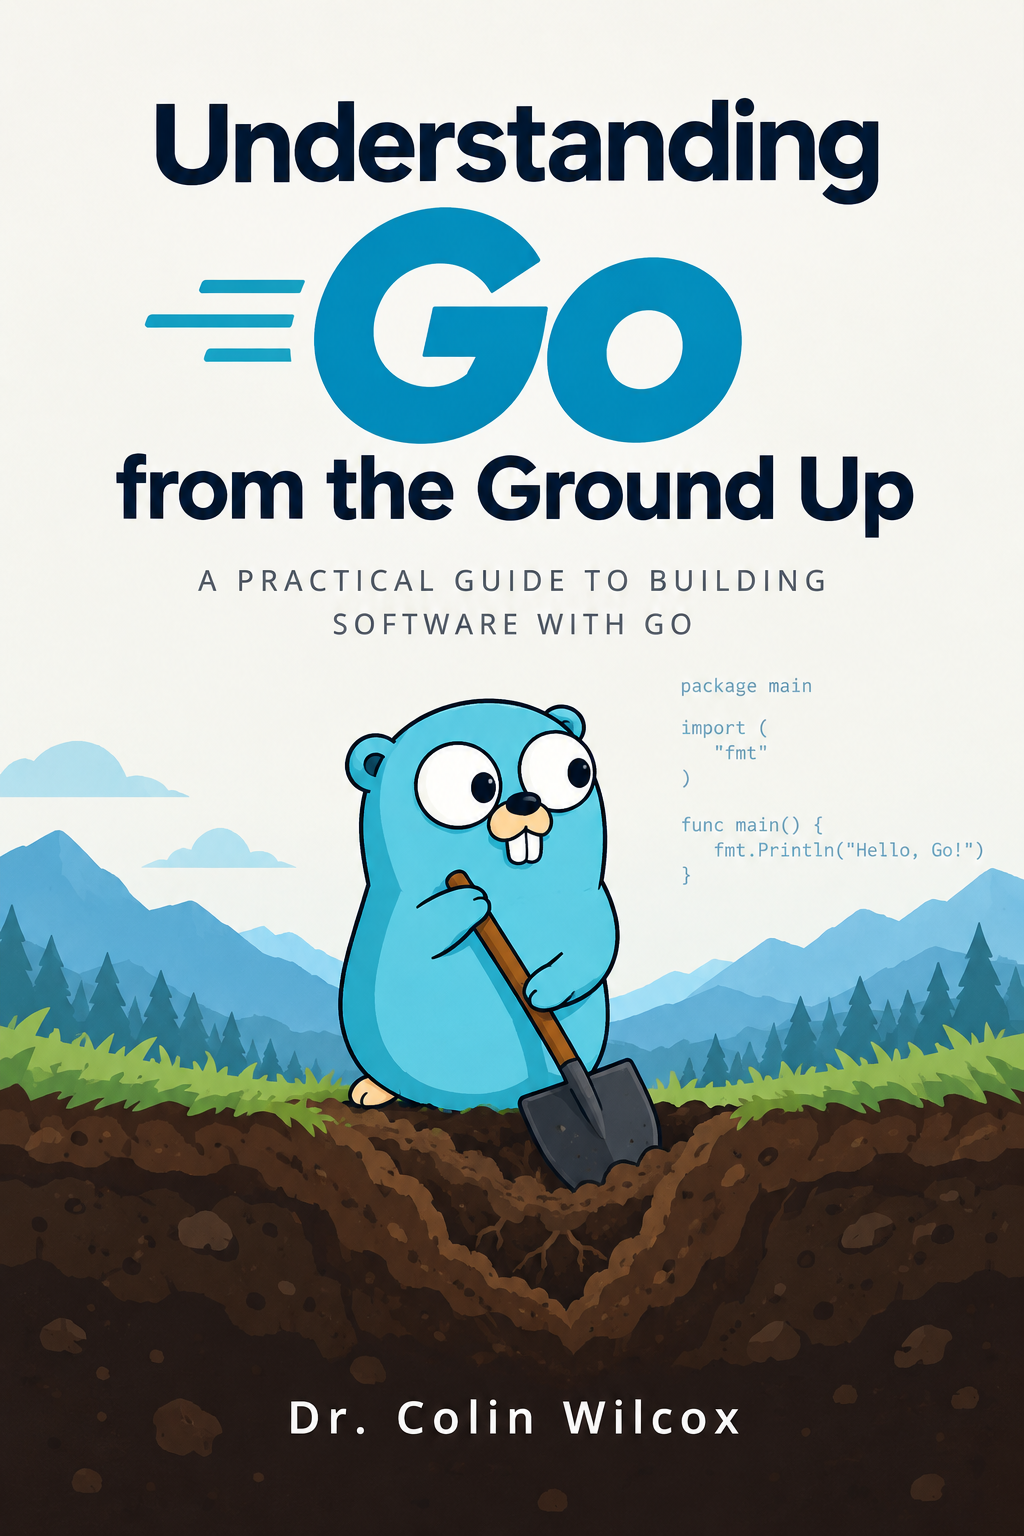
\includegraphics[width=\paperwidth,height=\paperheight]{images/cover.png}
    }

    \vspace*{0.65\paperheight}

%    \begin{center}
%        {\Huge \bfseries \color{white} Understanding Go from the Ground Up \par}
%        \vspace{1cm}
%        {\Large \color{white} Dr. Colin Wilcox \par}
%    \end{center}

\end{titlepage}

\ClearShipoutPictureBG
\maketitle
\tableofcontents

\mainmatter

% =========================================================
\part{Foundations: Starting from Zero}

\chapter{What Is Programming?}
\begin{chaptersummary}
Computers process, store and communicate information by following instructions provided by software. The CPU performs operations on binary data, while memory, storage and the operating system manage the data and resources needed to run applications. Complex tasks are achieved by combining many simple operations into sophisticated hardware and software systems.
\end{chaptersummary}

\section{What Computers Do ?}

At a high level, a computer is a programmable electronic system that receives data, processes them according to a set of instructions, stores information, and produces results. Although modern computers perform an enormous variety of tasks, from running websites and analysing scientific data to controlling industrial systems, these activities can ultimately be understood as different forms of information processing. \\


The fundamental operation of a computer is the execution of instructions. Software provides these instructions in the form of programs, while hardware provides the physical components needed to execute them. A program might instruct a computer to perform calculations, compare values, move data between locations, communicate over a network, or respond to user input.\\

The central processing unit (CPU) is the centre of most computers. The CPU repeatedly retrieves instructions from memory, interprets them, and performs the required operations. These operations are ultimately carried out using electronic circuits that manipulate binary values—represented conceptually as zeros and ones. Simple operations such as addition, comparison, and logical operations can be combined into increasingly complex sequences, allowing software to perform sophisticated tasks. \\

Computers also rely heavily on memory and storage. Main memory, or RAM, provides relatively fast temporary storage for the programs and data currently being used. Persistent storage, such as solid-state drives, retains data when the computer is switched off. The operating system manages these resources and provides common services through which applications can interact with hardware without having to directly control each physical component. \\

Input and output allow a computer to interact with the outside world. Input can come from devices such as keyboards, cameras, sensors, or network connections, while output can be presented through displays, speakers, actuators, or other connected systems. Internally, hardware components communicate through electronic interconnections and communication protocols, allowing data to move between processor, memory, storage, and peripheral devices. \\

At a higher level, the operating system coordinates these activities. Manage processes, memory, files, devices, and access to system resources. Applications such as web browsers, word processors and games operate above this layer, using operating-system services and software libraries rather than directly controlling the underlying hardware in most cases.\\

Modern computers also perform substantial work outside the individual machine. Through computer networks and the Internet, a device can exchange data with other computers and access remote services. In cloud computing, for example, an application may rely on processing and storage provided by large remote data centres rather than performing every operation locally.\\

The key idea is therefore that computers transform information through a hierarchy of abstraction. At the lowest level, electronic circuits manipulate binary states. These circuits implement processor instructions, which are combined into machine-level programs. Operating systems and software libraries provide higher-level abstractions, and applications use those abstractions to implement useful functionality.\\

Consequently, what appears to a user as a complex operation—such as editing a photograph, searching the Internet, or playing a video—is ultimately a very large sequence of relatively simple operations on data. The power of computing comes not primarily from any single operation, but from the speed, precision, and scale with which computers can execute these operations and combine them into increasingly sophisticated systems.
\section{Programming Languages Overview}
The history of modern computer programming languages is closely related to the evolution of computer technology itself. As computers became faster, smaller, and more powerful, programmers needed better ways to communicate with them. Early computers required programmers to write instructions directly in binary machine code, a process that was slow, error-prone, and difficult to maintain. Over time, programming languages evolved to become more readable, portable, and expressive, allowing developers to build increasingly sophisticated software.\\

Today, there are hundreds of programming languages, each designed to solve particular types of problem. The development of these languages reflects decades of innovation in computer science, software engineering, and mathematics.

\subsection{The Era of Machine Language (1940s--1950s)}

The first electronic computers, including systems such as ENIAC and UNIVAC, were programmed using machine language. Machine language consists entirely of binary numbers (0s and 1s) that correspond directly to instructions executed by the computer's processor.\\

For example, a simple operation such as adding two numbers required programmers to know the exact binary instruction codes and memory addresses. Programs were often entered using switches, punch cards, or paper tape.\\

Programming at this level presented several challenges:

\begin{itemize}
    \item Programs were extremely difficult to understand.
    \item Even small errors could cause complete program failure.
    \item Programs written for one computer rarely worked on another.
    \item Development was slow and expensive.
\end{itemize}

Because of these limitations, programmers sought methods that would make software development easier.\\

\subsection{Assembly Language}

Assembly language was introduced during the early 1950s as a symbolic representation of machine code. Instead of remembering binary instruction patterns, programmers could use mnemonic commands such as:

\begin{itemize}
    \item \texttt{MOV} (move data)
    \item \texttt{ADD} (addition)
    \item \texttt{SUB} (subtraction)
    \item \texttt{JMP} (jump to another instruction)
\end{itemize}

An assembler translated these human-readable commands into machine code.\\

Assembly language dramatically improved programmer productivity while maintaining complete control over hardware. It became particularly important for operating systems, embedded systems, and device drivers.\\

However, the assembly language remained hardware-specific. A program written for one processor architecture usually had to be rewritten for another.\\

\subsection{The Birth of High-Level Programming Languages}

The greatest leap forward came with the invention of high-level programming languages during the 1950s. These languages allowed programmers to describe algorithms using words, mathematical expressions, and logical structures rather than processor instructions. Compilers translated high-level languages into machine code. \\

\subsubsection{FORTRAN}

Released in 1957, FORTRAN (Formula Translation) was one of the first successful high-level programming languages.\\

Developed by IBM, FORTRAN focused on scientific and engineering calculations. It introduced features such as:

\begin{itemize}
    \item Variables
    \item Loops
    \item Conditional statements
    \item Mathematical expressions
    \item Functions
\end{itemize}

FORTRAN enabled scientists and engineers to solve complex numerical problems much more quickly than before and remained a dominant scientific programming language for decades.

\subsubsection{COBOL}

COBOL (Common Business-Orientated Language) was introduced in 1959 to meet the needs of businesses and governments.\\

Unlike FORTRAN, COBOL emphasised readability. Its syntax resembled English sentences, making programs easier for managers and analysts to understand.

COBOL became widely used for:

\begin{itemize}
    \item Banking
    \item Payroll
    \item Accounting
    \item Government databases
    \item Insurance systems
\end{itemize}

Many legacy financial systems around the world continue to use COBOL today.

\subsection{Structured Programming (1960s--1970s)}

As software projects became larger, programmers discovered that unrestricted jumps (using the \texttt{goto} statement) made programs difficult to understand.\\

Researchers promoted structured programming, a methodology that encouraged programs to be built using:

\begin{itemize}
    \item Sequence
    \item Selection (\texttt{if} statements)
    \item Iteration (loops)
\end{itemize}

This approach improved readability, testing, and maintenance.

\subsection{ALGOL}

ALGOL introduced many concepts that later became standard in programming languages, including:

\begin{itemize}
    \item Block structure
    \item Nested scopes
    \item Formal syntax descriptions
    \item Recursive procedures
\end{itemize}

Although ALGOL itself was not widely used commercially, it heavily influenced future languages.

\subsection{Pascal}

Niklaus Wirth designed Pascal in 1970 primarily for education. Pascal emphasised:

\begin{itemize}
    \item Clear syntax
    \item Strong type checking
    \item Structured programming
    \item Program organisation
\end{itemize}

For many years, Pascal became the primary language used to teach programming in universities.

\subsection{The Rise of C}

One of the most influential programming languages ever created was C. Developed by Dennis Ritchie at Bell Laboratories in the early 1970s, C balanced high-level programming with direct access to computer hardware.\\

C introduced features such as:

\begin{itemize}
    \item Pointers
    \item Efficient memory management
    \item Portable compilers
    \item Modular programming
\end{itemize}

Perhaps its greatest achievement was enabling the Unix operating system to be rewritten in a portable language rather than assembly language.\\

Today, C remains widely used in:

\begin{itemize}
    \item Operating systems
    \item Embedded devices
    \item Game engines
    \item Databases
    \item Networking software
\end{itemize}

Many modern languages borrow syntax directly from C.

\subsection{Object-Oriented Programming}

By the 1980s, software systems had grown into millions of lines of code. Managing this complexity required new programming techniques.\\

Object-orientated programming (OOP) organised software around objects that combine data with the operations that manipulate those data.\\

The four major principles of object-orientated programming are as follows.

\begin{itemize}
    \item Encapsulation
    \item Inheritance
    \item Polymorphism
    \item Abstraction
\end{itemize}

These ideas helped programmers design reusable and maintainable software.

\subsection{C++}

Created by Bjarne Stroustrup, C++ extended C with object-orientated features while retaining high performance.\\

C++ became popular for:

\begin{itemize}
    \item Video games
    \item Financial software
    \item Desktop applications
    \item Simulation software
    \item Operating systems
\end{itemize}

\subsection{Java}

Java, introduced by Sun Microsystems in 1995, revolutionised software portability.\\

Instead of compiling directly to machine code, Java programs compile into bytecode that runs on the Java Virtual Machine (JVM). This approach led to Java's famous slogan:

\begin{quote}
\textbf{``Write Once, Run Anywhere.''}
\end{quote}

Java became a leading language for:

\begin{itemize}
    \item Enterprise software
    \item Android development
    \item Large-scale server applications
    \item Web services
\end{itemize}

\subsection{The Internet Revolution}

The rapid growth of the Web during the 1990s transformed programming.

\subsection{JavaScript}

Originally created in only ten days by Brendan Eich, JavaScript enabled interactive websites. \\

Instead of static pages, websites could now include the following:

\begin{itemize}
    \item Dynamic menus
    \item Animations
    \item Online forms
    \item Interactive maps
    \item Browser games
\end{itemize}

Today, JavaScript powers nearly all modern websites.

\subsection{PHP}

PHP simplified web server programming and became the foundation for many early dynamic websites and content management systems, including WordPress.

\subsection{Perl}

Perl became popular for system administration, text processing, and early web development due to its powerful pattern-matching capabilities.

\subsection{Python and Simplicity}

Python was created by Guido van Rossum in 1991 with the goal of making programming simple and readable.\\

Python emphasises:

\begin{itemize}
    \item Clean syntax
    \item Minimal boilerplate code
    \item Extensive standard libraries
    \item Cross-platform compatibility
\end{itemize}

Because beginners can learn it quickly while professionals can build complex applications, Python has become one of the world's most popular programming languages.\\

Its major applications include

\begin{itemize}
    \item Artificial intelligence
    \item Machine learning
    \item Data science
    \item Scientific computing
    \item Robotics
    \item Automation
    \item Web development
    \item Cybersecurity
\end{itemize}

\subsection{Functional Programming}

Although functional programming concepts originated decades earlier, they became increasingly influential in modern software development.\\

Languages such as Haskell, Scala, Elixir, and F \# emphasise:

\begin{itemize}
    \item Immutable data
    \item Pure functions
    \item Higher-order functions
    \item Reduced side effects
\end{itemize}

Functional programming often makes concurrent and parallel programs easier to reason about.

\subsection{Modern Programming Languages}

Since 2000, new languages have addressed challenges such as cloud computing, multicore processors, and cybersecurity.

\subsection{C\#}

Developed by Microsoft, C \# combines object-orientated programming with modern language features and is widely used for enterprise applications, desktop software, web development, and game development through Unity.

\subsection{Go}

Created by Google, Go focuses on simplicity, concurrency, and fast compilation.\\

It is widely used for:

\begin{itemize}
    \item Cloud computing
    \item Distributed systems
    \item Networking
    \item Container technologies
\end{itemize}

\subsection{Rust}

Rust addresses one of programming's oldest problems: memory safety. Its ownership system prevents many common programming errors without requiring a garbage collector.\\

Rust has gained popularity in:

\begin{itemize}
    \item Operating systems
    \item Web browsers
    \item Embedded programming
    \item Security-critical software
\end{itemize}

\subsection{Swift}

Apple introduced Swift to replace Objective-C to develop applications on macOS, iOS, watchOS, and tvOS.\\

Swift emphasises safety, speed, and modern programming practices.

\subsection{Kotlin}

Kotlin became Google's preferred language for Android development due to its concise syntax and improved safety compared to Java.

\subsection{TypeScript}

TypeScript extends JavaScript by adding static typing and improved development tools. Large web applications increasingly rely on TypeScript because it reduces programming errors while remaining fully compatible with JavaScript.

\subsection{Current Trends}

Modern programming language design continues to evolve in response to new technologies. \\

Current trends include:

\begin{itemize}
    \item Improved memory safety
    \item Better concurrency support
    \item Integration of artificial intelligence
    \item Cloud-native development
    \item Cross-platform programming
    \item Automatic memory management
    \item Strong static typing
    \item Developer productivity
\end{itemize}

Language designers increasingly prioritise writing reliable, maintainable, and secure software rather than simply maximising execution speed.

\subsection{Summary}

The evolution of programming languages reflects the broader history of computing. Each generation of languages has sought to overcome the limitations of its predecessors by making programming more intuitive, portable, efficient, and secure. From binary machine code to today's sophisticated languages, developers have continually improved the tools used to communicate with computers.\\

Modern programmers can choose from a diverse ecosystem of languages, each optimised for different domains, including systems programming, web development, mobile applications, artificial intelligence, scientific research, and cloud computing. As computing technologies continue to advance, programming languages will continue to evolve, incorporating new paradigms and features that make software development more accessible and capable of addressing the increasingly complex challenges of the digital age.

\section{Why Develop Software in Go?}
Go, also known as Golang, was developed by Google and first released publicly in 2009. It was designed to address challenges associated with large-scale software development, particularly long compilation times, complex dependency management, and the difficulty of writing concurrent systems in some established languages. Since its introduction, Go has evolved into a mature general-purpose programming language with improvements to its compiler, tooling, standard library, and language features. A significant development was the introduction of generics in Go 1.18, which provided greater flexibility for reusable code while retaining Go's emphasis on simplicity.\\

Go is particularly well suited for modern systems and backend development because it combines relatively simple syntax with strong static typing, efficient compilation, and built-in support for concurrency through goroutines and channels. Its standard toolchain also provides integrated facilities for formatting, testing, dependency management, and building applications, reducing the need for extensive external tooling. Go produces compiled binaries and has efficient runtime performance, making it suitable for services, cloud infrastructure, networking applications, and distributed systems.\\

Developing in Go can therefore provide a balance between developer productivity and system performance. Its deliberately small language design makes code relatively easy to read and maintain, while its concurrency model and cross-platform compilation support modern distributed applications. Although Go is not the best choice for all types of software, its simplicity, strong tooling, performance, and suitability for scalable systems make it a practical choice for developing reliable and maintainable applications.

\chapter{Setting Up Your Environment}
\begin{chaptersummary}
This chapter introduces the steps required to set up a Go (Golang) development environment, providing a solid foundation for writing, running, and managing Go applications. It covers installing the Go compiler and toolchain, configuring environment variables, setting up a suitable code editor or IDE, and understanding the basic project structure. Through practical examples, readers will learn how to verify their installation, create their first Go program, and execute it from the command line. By the end of this chapter, readers will have a fully functional Go development environment and be ready to begin building their own Go applications.
\end{chaptersummary}

\section{Setting Up a Clean Go Development Environment}

A clean Go development environment should provide the Go compiler and toolchain, a suitable code editor, dependency management, testing facilities, and version-control support. The environment should also be configured so that projects remain isolated from the operating system and can be reproduced on other development machines. The following procedure describes a suitable setup for both Windows and Linux.

\subsection{Installing Go}

The first step is to install the official Go distribution. Go should be installed from the official Go distribution rather than from an unverified third-party source. The installation provides the Go compiler, standard library, command-line tools, and supporting utilities required to build and test Go programs.

\subsubsection{Windows}

On Windows, the Go installer can be downloaded from the official Go website. The installer places the Go distribution in the standard installation directory and configures the required environment variables. Once installation is complete, a new PowerShell or Command Prompt session should be opened so that the updated environment is available.\\

The installation can be verified using:

\begin{lstlisting}
go version
\end{lstlisting}

A successful installation should return the installed Go version and the target platform. Additional information about the Go environment can be obtained using:

\begin{lstlisting}
go env
\end{lstlisting}

The \texttt{go env} output can be useful for diagnosing problems related to the Go installation, the module cache, the compiler, or the executable search path.

\subsubsection{Linux}

On Linux, Go can be installed using the distribution's package manager or by downloading the official Go archive. For development environments where a specific Go version is required, installing the official distribution is often preferable because it provides direct control over the installed version.\\

After installation, the Go executable should be available through the system's \texttt{PATH}. This can be checked with:

\begin{lstlisting}
go version
\end{lstlisting}

The installation can also be inspected using:

\begin{lstlisting}
go env
\end{lstlisting}

If Go was installed manually, the relevant Go binary directory should be added to the user's \texttt{PATH}. For example, a typical shell configuration might contain:

\begin{lstlisting}
export PATH=$PATH:/usr/local/go/bin
\end{lstlisting}

The exact configuration depends on the installation method and Linux distribution.

\subsection{Choosing a Project Location}

Go projects should be stored in a dedicated development directory rather than directly inside the Go installation directory. For example, a developer might create a directory called \texttt{Projects} in their home directory.\\

On Linux, this could be:

\begin{lstlisting}
mkdir -p ~/Projects
cd ~/Projects
\end{lstlisting}

On Windows PowerShell, an equivalent directory can be created using:

\begin{lstlisting}
New-Item -ItemType Directory -Path "$HOME\Projects"
Set-Location "$HOME\Projects"
\end{lstlisting}

Keeping source code separate from the Go installation makes the environment easier to maintain and prevents project files from becoming mixed with compiler or standard-library files.

\subsection{Using Go Modules}

Modern Go development should use Go modules for dependency management and version management. A module defines the identity of a project and records the dependencies required to build it. This approach avoids the need to place the source code of the application in a specific global workspace.\\

A new project can be created by making a directory and initialising a module:

\begin{lstlisting}
mkdir example
cd example
go mod init example
\end{lstlisting}

For a real project, the module path would normally correspond to the project's repository location. For example:

\begin{lstlisting}
go mod init github.com/example/example
\end{lstlisting}

The command creates a \texttt{go.mod} file. This file should be put into version control because it defines the module and records important dependency information.

When dependencies are added, Go can update the module files automatically. The command:

\begin{lstlisting}
go mod tidy
\end{lstlisting}

can be used to remove unnecessary dependencies and add dependencies required by the source code.

\subsection{Creating a Minimal Go Program}

A clean environment should be tested with a small application before development begins. A file named \texttt{main.go} can be created that contains:

\begin{lstlisting}
package main

import "fmt"

func main() {
    fmt.Println("Hello, Go!")
}
\end{lstlisting}

The program can be executed without first creating a separate executable using:

\begin{lstlisting}
go run .
\end{lstlisting}

If the environment is configured correctly, the program will compile and display:

\begin{lstlisting}
Hello, Go!
\end{lstlisting}

The application can also be compiled using:

\begin{lstlisting}
go build
\end{lstlisting}

This produces an executable suitable for the current operating system and architecture.

\subsection{Selecting an Integrated Development Environment}

Although Go can be developed entirely from the command line, an integrated development environment (IDE) or capable code editor can improve productivity. Visual Studio Code is a common choice because it provides editing, syntax highlighting, code navigation, debugging, testing, and integration with the Go toolchain.\\

After installing Visual Studio Code, the official Go extension can be installed. The extension provides features such as automatic formatting, code completion, diagnostics, testing support, debugging, and navigation between declarations.\\

The Go formatter should be used consistently. Go provides the \texttt{gofmt} utility, which formats the Go source code according to the standard Go formatting conventions. A source file can be formatted using the following:

\begin{lstlisting}
gofmt -w main.go
\end{lstlisting}

Using a common formatting standard reduces unnecessary differences between source files and makes collaborative development easier.

\subsection{Installing Development Tools}

The Go toolchain includes several commands that support the software development lifecycle. Some of the most important commands are shown below.

\begin{lstlisting}
go run .
go build
go test ./...
go fmt ./...
go vet ./...
go mod tidy
\end{lstlisting}

The \texttt{go test ./...} command executes tests throughout the module. The \texttt{go vet ./...} command performs additional static analysis and can identify certain classes of programming error.\\

A clean development workflow should run formatting, testing, and static analysis regularly, particularly before the code is committed to version control.

\subsection{Testing the Development Environment}

Go has built-in support for unit testing. A test file usually has the suffix \texttt{\_test.go}. For example, a simple test could be placed in \texttt{main_test.go}:

\begin{lstlisting}
package main

import "testing"

func TestExample(t *testing.T) {
    expected := "Hello, Go!"

    if expected != "Hello, Go!" {
        t.Errorf("unexpected result")
    }
}
\end{lstlisting}

Tests can be executed using:

\begin{lstlisting}
go test ./...
\end{lstlisting}

For larger projects, the test suite should be executed automatically as part of the development and integration process.

\subsection{Version Control}

Git should normally be used to manage the source code of a Go project. A new repository can be initialised with:

\begin{lstlisting}
git init
\end{lstlisting}

The repository should contain the source code \texttt{go.mod} and, where appropriate, \texttt{go.sum}. Build output, editor-specific configuration, temporary files, and other generated content should generally not be committed.\\

A suitable \texttt{.gitignore} file can be used to prevent unwanted files from being added to the repository. The precise contents depend on the project and development tools being used.

\subsection{Managing Dependencies}

Go's module system provides a controlled mechanism for managing external dependencies. A dependency can be added using:

\begin{lstlisting}
go get example.com/some/package
\end{lstlisting}

The dependency is then recorded in the module's dependency information. Developers should avoid manually copying third-party source code into a project when a properly versioned Go module is available.

The dependency graph can be maintained with:

\begin{lstlisting}
go mod tidy
\end{lstlisting}

This helps keep the project configuration clean and ensures that required and unused dependencies are accurately represented.

\subsection{Cross-Platform Development}

One of Go's significant advantages is its support for cross-platform compilation. A program developed on Windows can, for example, be compiled for Linux by specifying the target operating system and architecture:

\begin{lstlisting}
GOOS=linux GOARCH=amd64 go build
\end{lstlisting}

In Windows PowerShell, the environment variables can instead be specified as

\begin{lstlisting}
$env:GOOS = "linux"
$env:GOARCH = "amd64"
go build
\end{lstlisting}

The exact target should be selected according to the system on which the resulting executable will run. This capability is particularly useful when applications are developed on Windows but deployed to Linux servers or containers.

\subsection{Keeping the Environment Clean}

A clean development environment should minimise unnecessary global configuration. Projects should use Go modules, dependencies should be explicitly versioned, and source code should remain separate from the Go installation. Developers should also avoid modifying the system-wide configuration unless necessary.\\

Go's module cache is managed automatically by the toolchain, so developers generally do not need to manually download or copy dependencies into individual projects. Similarly, Go applications should normally be built using the project's module definition rather than relying on manually configured library paths.\\

It is also good practice to keep the Go version consistent across a development team. The required version can be specified in the project's \texttt{go.mod} file, allowing developers and automated build systems to identify the expected language and toolchain version.\\

\subsection{Recommended Development Workflow}

Once the environment has been configured, a typical development workflow is:

\begin{enumerate}
    \item Create or clone the project repository.
    \item Initialise or verify the Go module.
    \item Open the project in the chosen editor or IDE.
    \item Implement the required functionality.
    \item Format the source code using \texttt{gofmt} or the editor's Go integration.
    \item Run the test suite using \texttt{go test ./...}.
    \item Run static analysis using \texttt{go vet ./...}.
    \item Run \texttt{go mod tidy} when dependencies change.
    \item Build the application using \texttt{go build}.
    \item Commit the source code and the module files to Git.
\end{enumerate}

Following this process provides a consistent development environment for both Windows and Linux. Separates application source code from the underlying Go installation, provides reproducible dependency management, and uses the standard Go tooling for formatting, testing, analysis, and compilation. The result is a development environment that is relatively simple to maintain, while remaining suitable for professional software development.
\section{Go Toolchain}
The Go toolchain is the collection of programs and commands used to
develop, build, test, analyse, and package programs written in the Go
programming language.  It is distributed with Go itself and is designed
to provide a standard and largely automated development workflow.\\

The main command is \texttt{go}.  Rather than requiring developers to
invoke a compiler, linker, archiver, test runner, and other tools
individually, the \texttt{go} command coordinates these components.\\

A typical workflow can be represented as

\textbf{
\[
\text{Source code}
\longrightarrow
\text{Packages}
\longrightarrow
\text{Compilation}
\longrightarrow
\text{Linking}
\longrightarrow
\text{Executable}
\]
}

with testing, formatting, dependency management, and analysis occurring
alongside these stages.

\subsection{Installing and Configuring Go}

The first step is to installing a Go distribution.  This provides the
compiler, standard library, \texttt{go} command, and supporting
development tools.\\

After installation, the command is executed.

\begin{lstlisting}
go version
\end{lstlisting}

can be used to verify that Go is available.\\

For example:

\begin{lstlisting}
$ go version
go version go1.25.0 linux/amd64
\end{lstlisting}

The exact version will depend on the installed release.

\subsection*{Why is this needed?}

The compiler and associated tools are required to transform Go source
code into executable programs.  The Go installation also provides the
standard library, which contains commonly used packages such as
\texttt{fmt}, \texttt{os}, \texttt{net/http}, and \texttt{encoding/json}.

\subsection{Creating a Go Module}

Modern Go projects normally use a Go module to define the project's
module path and manage dependencies.\\

A module can be created with this feature.

\begin{lstlisting}
go mod init example.com/hello
\end{lstlisting}

This creates a file named \texttt{go.mod}.  A simplified example is as follows:

\begin{lstlisting}
module example.com/hello

go 1.25
\end{lstlisting}

The module path identifies the project and provides the namespace used
when importing packages belonging to the module.

\subsection*{Why is this needed?}

A Go program may consist of many packages and may depend on packages
provided by other modules.  The module system gives enough information for the Go toolchain  to determine which dependencies are required and
which versions should be used.\\

For example, a project might have the following structure:

\begin{lstlisting}
hello/
|-- go.mod
|-- main.go
|-- internal/
|   `-- greeting/
|       `-- greeting.go
\end{lstlisting}

The \texttt{go.mod} file establishes the root of the module and allows
the toolchain to resolve imports consistently.

\subsection{Writing Go Source Code}

Go programs are normally organised into packages.  The simplest
executable program belongs to the \texttt{main} package and contains a
\texttt{main} function.\\

For example:

\begin{lstlisting}
package main

import "fmt"

func main() {
    fmt.Println("Hello, world!")
}
\end{lstlisting}

The source file can be saved as \texttt{main.go}.

\subsection*{Why is this needed?}

The source code expresses the behaviour of the program.  The Go
toolchain operates on packages rather than treating every source file
as an entirely independent compilation unit.\\

Files belonging to the same package are compiled together.  This allows
the compiler to perform type checking and determine relationships
between declarations within the package.

\subsection{Formatting the Source Code}

Go provides a standard formatter through

\begin{lstlisting}
gofmt
\end{lstlisting}

or, more commonly,

\begin{lstlisting}
go fmt ./...
\end{lstlisting}

For example, code such as

\begin{lstlisting}
func main(){fmt.Println("Hello")}
\end{lstlisting}

will be formatted in the conventional Go style:

\begin{lstlisting}
func main() {
    fmt.Println("Hello")
}
\end{lstlisting}

\subsection*{Why is this needed?}

Formatting is not required for the compiler to understand valid Go
programmes, but it is important for consistency.  Go deliberately has a
strong standard formatting convention.\\

This means that different developers and projects generally use the
same layout, reducing unnecessary arguments about indentation,
braces, spacing, and similar stylistic details.

\subsection{Resolving Dependencies}

If a project imports a package from another module, the Go toolchain
must locate the required module version.

For example:

\begin{lstlisting}
import "example.com/some/library"
\end{lstlisting}

The required dependency is recorded in \texttt{go.mod}.  The command

\begin{lstlisting}
go mod tidy
\end{lstlisting}

can be used to ensure that the module files accurately describe the
dependencies used by the project.\\

The toolchain may also create or update \texttt{go.sum}, which contains
checksums used to verify the downloaded module content.

\subsection*{Why is this needed?}

A compiler cannot compile an import that it cannot locate.  Dependency
resolution therefore establishes the set of packages that are required
before compilation can take place.\\

The module system also makes builds more reproducible by recording
dependency versions rather than relying solely on whatever happens to
be installed on a developer's machine.

\subsection{Loading and Analysing Packages}

When a command such as

\begin{lstlisting}
go build
\end{lstlisting}

When executed, the Go toolchain first determines which packages are
involved and how they depend on one another.\\

For example:

\begin{lstlisting}
main
 |
 +-- internal/greeting
 |
 `-- fmt
\end{lstlisting}

The toolchain constructs the relevant package dependency graph.

\subsection*{Why is this needed?}

The compiler must know which source files belong to each package and
which imported packages are required.  The dependency graph also
allows independent packages to be compiled separately and, where
appropriate, in parallel.

\subsection{Type Checking}

The Go compiler analyses the source code and checks that it obeys the
rules of the Go language.\\

For example:

\begin{lstlisting}
var number int
number = "hello"
\end{lstlisting}

is invalid because a value of type \texttt{string} is being assigned to
a variable of type \texttt{int}.\\

The compiler reports an error rather than producing a normal executable.

\subsection*{Why is this needed?}

Type checking detects many programming errors before the programme is
run.  Go is statically typed, so the compiler can determine many
properties of a program during compilation.

This is one of the reasons for the simplicity of a simple command such as

\begin{lstlisting}
go build
\end{lstlisting}

can catch substantial classes of programming errors.

\subsection{Compiling Packages}

After source analysis and type checking, the Go compiler translates the
source code into compiled object information.\\

Conceptually:

\[
\text{Go source}
\longrightarrow
\text{compiled package}
\]

The compiler is normally invoked indirectly through the \texttt{go}
command rather than being called manually.

For example:

\begin{lstlisting}
go build
\end{lstlisting}

causes the necessary packages to be compiled.

\subsection*{Why is this needed?}

The source code is written for humans and expresses the programme behaviour in the
Go language.  The processor cannot directly execute Go source code.
Compilation translates it into a form suitable for subsequent linking
and execution.\\

The compiler also performs important optimisations and generates
machine code appropriate for the selected target architecture.

\subsection{Linking}

An executable program normally consists of more than the code written
in \texttt{main.go}.  It may depend on many packages, including
packages from the standard library.\\

The linker combines the required compiled components into an executable
program.\\

Conceptually:

\[
\text{compiled packages}
\longrightarrow
\text{linker}
\longrightarrow
\text{executable}
\]

For example:

\begin{lstlisting}
go build -o hello
\end{lstlisting}

can produce an executable named \texttt{hello}.

\subsection*{Why is this needed?}

Compilation produces code for individual packages, whereas an
executable needs to contain the program as a complete linked unit.\\

The linker resolves references between the compiled components and
constructs the final executable image.

\subsection{Building the Program}

The command

\begin{lstlisting}
go build
\end{lstlisting}

coordinates the previous stages.

A simplified model is as follows:

\begin{enumerate}[label=\arabic*.]
    \item Load the module and packages.
    \item Resolve required dependencies.
    \item Compile packages that need compiling.
    \item Link the required components.
    \item Produce an executable when appropriate.
\end{enumerate}

For example:

\begin{lstlisting}
go build -o hello
./hello
\end{lstlisting}

might produce:

\begin{lstlisting}
Hello, world!
\end{lstlisting}

\subsection*{Why is this needed?}

\texttt{go build} provides a convenient abstraction over the compiler
and linker.  Developers normally do not need to know the exact compiler
or linker command required for every package in the program.

\subsection{Running Without Explicitly Building}

Go also provides:

\begin{lstlisting}
go run .
\end{lstlisting}

This builds the necessary program and runs it.

For a small program, one can therefore write:

\begin{lstlisting}
go run main.go
\end{lstlisting}

\subsection*{Why is this needed?}

\texttt{go run} is particularly convenient during development when the
developer wants to execute a program without keeping a separately
managed executable.\\

It should not be interpreted as meaning that the Go source code is directly
executed by the processor.  The necessary compilation still occurs.

\subsection{Testing}

Go has testing support built into its toolchain.  Tests are commonly
placed in files ending in \texttt{\_test.go}.\\

For example:

\begin{lstlisting}
func Add(a, b int) int {
    return a + b
}
\end{lstlisting}

could be tested with:

\begin{lstlisting}
func TestAdd(t *testing.T) {
    if Add(2, 3) != 5 {
        t.Fatal("expected 5")
    }
}
\end{lstlisting}

Tests can be executed using:

\begin{lstlisting}
go test ./...
\end{lstlisting}

Compilation tells us that the program is syntactically and
type-theoretically valid, but it does not prove that the program
produces the desired results.\\

Tests provide executable checks of the program's behaviour. The distinction is important:

\[
\text{Compilation} \neq \text{Correctness}
\]

A program can compile successfully and still contain serious logical
errors.

\subsection{Static Analysis}

Go also provides analysis tools that inspect source code without
executing the program.

A commonly used command is:

\begin{lstlisting}
go vet ./...
\end{lstlisting}

It can identify certain suspicious or incorrect programming constructs.

\subsection*{Why is this needed?}

Some problems are difficult or impossible to identify simply by
checking whether the programme compiles.  Static analysis can identify
patterns that are legal Go but are likely to indicate a programming
mistake.

Thus, a typical quality-orientated workflow is as follows.

\[
\text{format}
\rightarrow
\text{build}
\rightarrow
\text{test}
\rightarrow
\text{analyse}
\]

\subsection{Cross Compilation}

One notable feature of the Go toolchain is straightforward
cross-compilation.\\

For example, a developer on Linux can build for another operating
system and architecture by setting environment variables such as
\texttt{GOOS} and \texttt{GOARCH}:

\begin{lstlisting}
GOOS=windows GOARCH=amd64 go build -o hello.exe
\end{lstlisting}

The resulting executable targets Windows on the AMD64 architecture.

\subsection*{Why is this needed?}

Software is often developed on one platform but deployed on another.
Cross-compilation allows a developer or build server to produce
binaries for deployment targets without necessarily running the build
on the target operating system.\\

Conceptually:

\[
\text{Development machine}
\xrightarrow{\text{Go toolchain}}
\text{Target executable}
\]

\subsection{Caching}

The Go toolchain maintains build caches.  When a package has already
been compiled and its relevant inputs have not changed, the toolchain
can reuse the cached result.\\

Large projects can contain many packages.  Recompiling every package
after every small source-code change would be unnecessarily expensive.\\

Caching therefore reduces build times while preserving correctness:
if an input that affects a package changes, the relevant package is
rebuilt.\\

\subsection{The Complete Development Cycle}

A practical Go development workflow can therefore be summarised as:

\begin{enumerate}
    \item \textbf{Initialise a module} using \texttt{go mod init}.
    \item \textbf{Write source code} organised into packages.
    \item \textbf{Format the code} using \texttt{gofmt} or
          \texttt{go fmt}.
    \item \textbf{Resolve dependencies} using the Go module system.
    \item \textbf{Compile and type-check} the packages.
    \item \textbf{Link} the compiled packages into an executable.
    \item \textbf{Run} the program using \texttt{go run} or the
          resulting executable.
    \item \textbf{Test} the program using \texttt{go test}.
    \item \textbf{Analyse} it using tools such as \texttt{go vet}.
    \item \textbf{Build for deployment}, potentially using
          cross-compilation.
\end{enumerate}

The relationship between these activities can be visualised as:

\[
\boxed{
\begin{array}{c}
\text{Go source files}\\
\downarrow\\
\text{Formatting}\\
\downarrow\\
\text{Package loading}\\
\downarrow\\
\text{Dependency resolution}\\
\downarrow\\
\text{Parsing and type checking}\\
\downarrow\\
\text{Compilation}\\
\downarrow\\
\text{Linking}\\
\downarrow\\
\text{Executable}
\end{array}}
\]

Testing and static analysis operate alongside this pipeline:

\[
\begin{array}{ccccc}
& \text{Source code} & & &\\
& \downarrow & & &\\
\text{Formatting} & \rightarrow & \text{Build} & \rightarrow &
\text{Executable}\\
& & \downarrow & &\\
& & \text{Tests} & &\\
& & \downarrow & &\\
& & \text{Static analysis} & &
\end{array}
\]

\subsection{Conclusion}

The Go toolchain is deliberately integrated.  The developer generally
interacts with the single \texttt{go} command rather than manually
coordinating separate compilation, linking, dependency-management,
testing, and packaging commands.\\

Its central purpose is to turn a collection of Go source files and
their dependencies into a reliable, executable programme while making
common development activities predictable and repeatable.\\

In simplified form:

\[
\boxed{
\text{Source}
\rightarrow
\text{Packages}
\rightarrow
\text{Type checking}
\rightarrow
\text{Compilation}
\rightarrow
\text{Linking}
\rightarrow
\text{Executable}
}
\]

with

\[
\boxed{
\text{Formatting}
\quad
\text{Testing}
\quad
\text{Static analysis}
\quad
\text{Dependency management}
}
\]

supporting the main build pipeline.
\section{Editors and IDEs}

Go is supported by a relatively broad range of integrated development environments (IDEs) and extensible text editors. Unlike some languages, however, Go does not require a heavyweight IDE: the standard Go toolchain provides a substantial set of command-line facilities for building, testing, formatting and analysing programs, whilst the official \texttt{gopls} language server supplies much of the functionality normally associated with an IDE.\\

The choice of development environment is therefore primarily a question of workflow, project complexity, and personal preference. The principal options are Visual Studio Code, GoLand, Vim/Neovim and, to a lesser extent, other editors such as Emacs and LiteIDE.\\

\subsection{Visual Studio Code}

\href{https://code.visualstudio.com/}{Visual Studio Code (VS Code)} is arguably the most widely used development environment for Go. The 2024 H2 Go Developer Survey reported that 66\% of the respondents used VS Code regularly, compared to 35\% for GoLand, making VS Code the clear leader in terms of reported usage.\\

Go support is provided principally by the official
\href{https://marketplace.visualstudio.com/items?itemName=golang.go}{Go extension}, maintained by the Go team. The extension integrates closely with \texttt{gopls}, the official Go language server, and provides IntelliSense, code navigation, diagnostics, refactoring, formatting, testing, and debugging.\\

A significant advantage of this architecture is that much of the functionality is provided by the same underlying Go tooling used by other editors. Consequently, developers can obtain a consistent development experience whilst retaining the comparatively lightweight and extensible nature of VS Code.\\

\begin{itemize}
\item \textbf{Advantages:}
\begin{itemize}
\item Free and available on Windows, macOS and Linux.
\item Excellent Go support through the official Go extension.
\item Strong integration with \texttt{gopls}, the Go language server.
\item Integrated testing and debugging.
\item Extensive ecosystem of extensions for containers, Kubernetes, Git, databases, and cloud platforms.
\item Good support for multi-language projects in which Go is used alongside other languages.
\item Relatively low barrier of entry compared to a traditional full-featured IDE.
\end{itemize}

\item \textbf{Disadvantages:}
\begin{itemize}
    \item Some functionality depends on extensions and external Go tools rather than being part of the core editor.
    \item The large extension ecosystem can result in configuration complexity.
    \item Resource consumption can increase substantially when many extensions are installed.
    \item Some advanced IDE functionality may require more manual configuration than in GoLand.
\end{itemize}

\end{itemize}

For most Go developers, VS Code is a strong default choice, particularly where a free, extensible, and multi-purpose development environment is required.\\

More information is available from the
\href{https://go.dev/doc/editors}{official Go editor documentation}
and the
\href{https://code.visualstudio.com/docs/languages/go}{VS Code Go documentation}.

\subsection{GoLand}

\href{https://www.jetbrains.com/go/}{GoLand}, developed by JetBrains, is a dedicated commercial IDE designed specifically for Go development. It is based on the IntelliJ platform and provIDE. a highly integrated development environment in which many features that require extensions or additional configuration in lighter editors are available as part of the IDE.\\

GoLand provides sophisticated code completion, navigation, refactoring, debugging, testing, profiling, and integration with Go modules. It also provides support for common technologies surrounding Go development, including version control systems, databases, HTTP clients, Docker and Kubernetes.\\

The principal distinction between GoLand and VS Code is therefore not whether either can provide the essential Go functionality, both are capable of this, but rather how much of the surrounding development workflow is integrated into the IDE itself.

\begin{itemize}
\item \textbf{Advantages:}
\begin{itemize}
\item Comprehensive, dedicated Go development environment.
\item Very strong code navigation and refactoring facilities.
\item Integrated debugging, testing and profiling.
\item Good support for Go modules and complex project structures.
\item Extensive integration with databases, containers, version control and other development tools.
\item Generally requires less extension-level configuration than VS Code.
\item Particularly well suited to large and complex commercial Go projects.
\end{itemize}

\item \textbf{Disadvantages:}
\begin{itemize}
    \item Commercial licences are required for many users.
    \item Heavier in terms of memory and system resources than a minimalist editor.
    \item Less attractive for developers who prefer a highly configurable, editor-centric workflow.
    \item Its breadth of functionality can be unnecessary for small Go programs or simple command-line utilities.
\end{itemize}

\end{itemize}

GoLand is therefore particularly attractive for professional teams working on sizeable Go codebases where sophisticated refactoring, debugging, and project-management facilities justify the additional resource requirements and licencing considerations.\\

It is worth noting that Go support is also available through the Go plugin for
\href{https://www.jetbrains.com/idea/}{IntelliJ IDEA Ultimate}; JetBrains states that the Go plugin provides the functionality available in GoLand. This can be advantageous for developers who already use the IntelliJ ecosystem for other languages.\\

More information is available from the
\href{https://www.jetbrains.com/go/}{GoLand product documentation}
and the
\href{https://www.jetbrains.com/help/idea/go-plugin.html}{IntelliJ IDEA Go documentation}.

\subsection{Vim and Neovim}

\href{https://www.vim.org/}{Vim} and
\href{https://neovim.io/}{Neovim} occupy a different position from conventional IDEs. They are highly configurable text editors that can be transformed into capable Go development environments through plugins and language-server integration.\\

The most important component is again \texttt{gopls}. Neovim provides native Language Server Protocol (LSP) facilities, whilst Vim can use a number of LSP-oriented plugins. The Go project provides specific guidance for configuring \texttt{gopls} with Vim and Neovim.\\

A typical configuration can provide completion, diagnostics, code navigation, formatting, import organisation, and other IDE-like facilities without abandoning the keyboard-driven Vim workflow.

\begin{itemize}
\item \textbf{Advantages:}
\begin{itemize}
\item Extremely fast and lightweight once configured.
\item Excellent keyboard-driven workflow.
\item Highly configurable and scriptable.
\item Particularly effective when working over SSH or on remote systems.
\item Excellent integration with command-line Go tooling.
\item No requirement to adopt a large graphical IDE.
\end{itemize}

\item \textbf{Disadvantages:}
\begin{itemize}
    \item Initial configuration can be considerably more complicated than VS Code or GoLand.
    \item IDE functionality depends on plugins and configuration choices.
    \item Debugging and project-management workflows can require additional setup.
    \item Less suitable for developers unfamiliar with modal editors.
\end{itemize}

\end{itemize}

Vim or Neovim is therefore particularly appropriate for experienced developers who value efficiency, customisation, and terminal-based workflows. It is less compelling as a first Go environment for developers who want a fully integrated graphical IDE immediately.\\

The official Go documentation contains 
\href{https://go.dev/gopls/editor/vim}{guide to using \texttt{gopls} with Vim and Neovim}.

\subsection{Emacs}

\href{https://www.gnu.org/software/emacs/}{Emacs} is another extensible editor capable of providing a sophisticated Go development environment. Go support can be built around \texttt{gopls} and the Language Server Protocol, commonly through packages such as \texttt{lsp-mode} or related LSP integrations.\\

Emacs is particularly powerful for developers who already use it as their primary environment, since Go development can be integrated with terminals, version control, documentation, project management, and other workflows within a single highly programmable environment.\\

Its main limitation is the same characteristic that makes it attractive: considerable configurability. Achieving a polished Go environment generally requires more configuration than using GoLand or the official VS Code extension.

\begin{itemize}
\item \textbf{Advantages:}
\begin{itemize}
\item Exceptionally extensible and programmable.
\item Strong LSP support through \texttt{gopls}.
\item Excellent terminal and version-control integration.
\item Well suited to developers who already use Emacs extensively.
\end{itemize}

\item \textbf{Disadvantages:}
\begin{itemize}
    \item Greater configuration overhead.
    \item Less immediately accessible to newcomers.
    \item A number of Go-specific features depend on third-party packages and configuration.
\end{itemize}

\end{itemize}

\subsection{LiteIDE and Other Editors}

\href{https://github.com/visualfc/liteide}{LiteIDE} is an open-source IDE specifically oriented towards Go. ProvIDE a simpler, more traditional IDE experience and includes features such as Go-aware editing and integration with Go tools.\\

However, LiteIDE is considerably less prominent than VS Code and GoLand in the contemporary Go ecosystem. The Go project's own documentation lists it among the available editors, but the latest Go Developer Survey indicates that usage is heavily concentrated around VS Code and GoLand, with Vim/Neovim and other editors occupying smaller niches.\\

Other editors, including Sublime Text, Zed and Kate, can also provide Go development facilities through language-server or editor integrations. These can be excellent choices for users who already prefer those environments, but they are generally less significant as dedicated Go IDE choices.

\subsection{Comparison}

Table~\ref{tab:go-ides} summarises the principal trade-offs.

\begin{table}[htbp]
\centering
\caption{Comparison of major development environments for Go}
\label{tab:go-ides}
\begin{tabular}{p{0.16\textwidth}p{0.20\textwidth}p{0.27\textwidth}p{0.27\textwidth}}
\hline
\textbf{Environment} & \textbf{Model} & \textbf{Advantages} & \textbf{Disadvantages} \
\hline
VS Code &
Extensible editor/IDE &
Free; excellent official Go extension; \texttt{gopls} integration; strong debugging and testing; extensive ecosystem &
Some functionality requires extensions; configuration can become complex; less integrated than a dedicated IDE \

GoLand &
Dedicated commercial IDE &
Excellent Go-specific tooling; advanced refactoring, debugging and profiling; strong project and database integration &
Commercial for many users; comparatively resource-intensive; potentially excessive for small projects \

Vim/Neovim &
Highly configurable editor &
Very fast; keyboard-centric; excellent terminal and remote-development workflow; highly customisable &
Steeper learning curve; significant configuration and plugin management; some IDE functionality requires manual setup \

Emacs &
Extensible editor &
Extremely programmable; strong LSP support; excellent integration with command-line workflows &
High configuration overhead; less immediately accessible; Go functionality is assembled from packages \

LiteIDE &
Dedicated open-source Go IDE &
Simple Go-focused environment; open source; relatively lightweight &
Much smaller ecosystem and user base; fewer integrations and less momentum than VS Code or GoLand \
\hline
\end{tabular}
\end{table}

\subsection{The Role of \texttt{gopls}}

An important consideration when comparing Go development environments is that the boundary between an ``IDE feature'' and the underlying Go tooling is relatively thin. The official \texttt{gopls} language server provides a common foundation for many editors.\\

\texttt{gopls} supplies facilities such as code completion, navigation, diagnostics, symbol information, refactoring, and code actions. This means that a developer moving between VS Code, Neovim, Emacs and other LSP-compatible environments can retain a substantial proportion of the same language intelligence.\\

This architecture is beneficial to the Go ecosystem because the editor choice does not necessarily imply choosing a completely different language-analysis implementation. The official VS Code extension, for example, uses \texttt{gopls} as its default backend for many IntelliSense, navigation, editing and diagnostic features.

\subsection{Recommendation}

For most developers, the choice can be reduced to three principal options.

\begin{enumerate}
\item \textbf{VS Code} is the best general-purpose choice. It is free, widely adopted, well supported by the Go team, and sufficiently powerful for both small projects and substantial production systems.

\item \textbf{GoLand} is the strongest choice when a fully integrated, dedicated IDE is preferred. It is particularly compelling for large commercial applications where advanced refactoring, debugging, profiling, and project integration are important.

\item \textbf{Vim or Neovim} is an excellent choice for experienced developers who prefer a highly customisable and terminal-centric environment, especially when remote development over SSH is common.\\

\end{enumerate}

The latest available Go Developer Survey provides useful evidence for this hierarchy: VS Code was regularly used by 66\% of respondents and GoLand by 35\%, whilst 33\% reported regularly using two or more editors. The latter figure is significant because it demonstrates that editor choice need not be exclusive; for example, a developer may use GoLand or VS Code for primary development while using Neovim or Vim for quick edits on remote systems.\\

Ultimately, the most important factor is not the IDE itself, but the quality of integration with the standard Go toolchain. A suitable environment should provide reliable access to \texttt{go}, \texttt{gofmt}, \texttt{go test}, the Go module system, \texttt{gopls} and, where required, a debugger such as Delve. On this basis, VS Code and GoLand currently offer the strongest combination of maturity, functionality, and ecosystem support, while Vim/Neovim and Emacs remain compelling alternatives for developers with established editor-centric workflows.

\subsection*{Further Information}

\begin{itemize}
\item \href{https://go.dev/doc/editors}{Go project: Editor plugins and IDEs}
\item \href{https://go.dev/wiki/IDEsAndTextEditorPlugins}{Go Wiki: Editors and IDEs}
\item \href{https://go.dev/blog/survey2024-h2-results}{Go Developer Survey 2024 H2 results}
\item \href{https://code.visualstudio.com/docs/languages/go}{VS Code: Go documentation}
\item \href{https://www.jetbrains.com/go/}{JetBrains GoLand}
\item \href{https://go.dev/gopls/}{Go language server (\texttt{gopls})}
\item \href{https://go.dev/gopls/editor/vim}{\texttt{gopls}: Vim and Neovim}
\end{itemize}

\chapter{Your First Go Program}
\begin{chaptersummary}
This chapter introduces readers to writing and running their first Go program, building on the development environment established in the previous chapter. It explores the basic structure of a Go application, including the package main declaration, importing packages, and defining the main() function as the program’s entry point. Through a simple “Hello, World!” example, readers will learn how to write Go code, save it in a source file, compile and execute the program, and understand the output. The chapter also introduces fundamental Go syntax and explains how each component contributes to the program’s execution. By the end of this chapter, readers will have gained the confidence to create, run, and begin experimenting with their own Go programs.
\end{chaptersummary}

}\section{Hello World}
This chapter is very short! It simply shows a simple Go program that displays the message \textbf{“Hello, world”} on the screen.\\

\begin{lstlisting}
package main
import "fmt"

func main() {
    fmt.Println("Hello, world")
}
\end{lstlisting}


\textbf{package main} declares that the program belongs to the main package. This is the package used for an executable Go program.\\

\textbf{import "fmt"} imports Go’s \textbf{fmt} package, which provides functions for formatted input and output.\\

func \textbf{main()} defines the program’s \textbf{main} function. This is where the execution of the program begins.\\

\textbf{fmt.Println("Hello, world!")} uses the \textbf{Println} function from the \textbf{fmt} package to print the text \textit{“Hello, world!”} to the screen.\\

Curly braces \textbf{\{ \}} mark the beginning and end of the main function.\\

The program demonstrates the basic structure of a Go program: defining a package, importing a package, creating a main function, and using a function to produce output.


% =========================================================
\part{Core Language Basics}

\chapter{Variables and Data Types}
\begin{chaptersummary}
This chapter introduces variables and data types in Go, providing readers with the fundamental knowledge needed to store, manage, and manipulate data in their programs. It explains how to declare and initialise variables using explicit type declarations and Go’s short variable declaration syntax, as well as how to use constants to represent values that remain unchanged. Readers will explore Go’s built-in data types, including integers, floating-point numbers, strings, booleans, and complex numbers, while learning how type inference and zero values work. The chapter also covers type conversion, the differences between related data types, and common mistakes to avoid when working with variables. Through practical examples, readers will develop a clear understanding of how Go handles data and gain the skills needed to write more reliable, readable, and effective Go programs.
\end{chaptersummary}
\section{Variables}

In Go (Golang), a variable is a named storage location used to hold a value
that can be accessed and changed while a program is running. Every variable
has a data type, which determines what kind of value it can store and how that
value is handled by the program.

Variables can be declared using the \texttt{var} keyword. For example:

\begin{lstlisting}
var age int
age = 25
\end{lstlisting}

This declares a variable called \texttt{age} with the \texttt{int} data type
and assigns it the value \texttt{25}. A variable can also be declared and
initialised at the same time:

\begin{lstlisting}
var age int = 25
\end{lstlisting}

Go can infer the data type from the assigned value, so the type can often be
omitted:

\begin{lstlisting}
var age = 25
\end{lstlisting}

Inside a function, Go also provides short variable declaration using the
\texttt{:=} operator:

\begin{lstlisting}
name := "Alice"
score := 95
\end{lstlisting}

The \texttt{:=} operator declares and initialises a new variable, with Go
automatically determining its data type. Short declarations are commonly used
within functions, whereas \texttt{var} is required when a variable needs to be
declared without an initial value or in certain package-level declarations.

Variables can have their values changed after declaration, provided that the
new value is compatible with their data type:

\begin{lstlisting}
score := 95
score = 100
\end{lstlisting}

Go is \textbf{statically typed}, meaning that the type of a variable is
determined at compile time and cannot normally be changed to an unrelated
type during execution. For example:

\begin{lstlisting}
age := 25
age = "twenty-five"    // Compilation error
\end{lstlisting}

This produces a compilation error because \texttt{age} was initially declared
as an integer and cannot subsequently be assigned a string.


\section{Data Types}

A data type defines the kind of data that a variable can contain. Go provides
several built-in data types, including numeric types, strings and Boolean
values. Choosing an appropriate data type helps the compiler determine how
values should be stored and what operations can be performed on them.


\subsection{Integer Types}

The \texttt{int} type is used for whole numbers without decimal places:

\begin{lstlisting}
var age int = 25
\end{lstlisting}

Go also provides explicitly sized integer types, such as \texttt{int8},
\texttt{int16}, \texttt{int32} and \texttt{int64}. The number indicates the
number of bits used to represent the integer.

Unsigned integer types, such as \texttt{uint}, \texttt{uint8} and
\texttt{uint64}, can only represent zero and positive values.


\subsection{Floating-Point Types}

The \texttt{float32} and \texttt{float64} types are used to represent numbers
containing decimal values:

\begin{lstlisting}
var temperature float64 = 21.5
\end{lstlisting}

The \texttt{float64} type provides greater precision than \texttt{float32}
and is commonly used when greater numerical precision is required.


\subsection{Strings}

The \texttt{string} type represents a sequence of characters:

\begin{lstlisting}
var name string = "Alice"
\end{lstlisting}

Strings can also be created using short variable declaration:

\begin{lstlisting}
message := "Hello, world!"
\end{lstlisting}

Strings are commonly used for text such as names, messages and user input.


\subsection{Boolean Values}

The \texttt{bool} type represents a logical value and can contain either
\texttt{true} or \texttt{false}:

\begin{lstlisting}
var loggedIn bool = true
\end{lstlisting}

Boolean variables are commonly used in conditional statements:

\begin{lstlisting}
if loggedIn {
    fmt.Println("User is logged in")
}
\end{lstlisting}


\subsection{Other Go Data Types}

Go also provides more complex data types, including arrays, slices, maps,
structs, pointers, interfaces and functions. These allow programs to
represent collections of values, structured records and more complex
relationships between data.

For example, a slice can store multiple values of the same type:

\begin{lstlisting}
numbers := []int{10, 20, 30}
\end{lstlisting}

A map stores values using keys:

\begin{lstlisting}
ages := map[string]int{
    "Alice": 25,
    "Bob":   30,
}
\end{lstlisting}

Go's strong and static type system allows many type-related errors to be
detected during compilation rather than when the program is running. This
helps improve the reliability and predictability of Go programs.

\chapter{Operators and Expressions}
\begin{chaptersummary}
This chapter explores operators and expressions in Go, explaining how to perform calculations, compare values, and make logical decisions within a program. Readers will learn about the different categories of operators, including arithmetic operators for mathematical calculations, comparison operators for evaluating relationships between values, logical operators for combining conditions, and assignment operators for updating variables. The chapter also introduces bitwise operators and increment and decrement operations, highlighting their practical applications and behaviour in Go. Through clear explanations and practical examples, readers will learn how to construct and evaluate expressions, understand operator precedence and associativity, and avoid common mistakes when combining operators. By the end of this chapter, readers will be able to use Go’s operators effectively to manipulate data, evaluate conditions, and build more expressive and reliable programs.
\end{chaptersummary}
\section{Operators and Expressions in the Go Programming Language}

Go, commonly referred to as Golang, is a statically typed,
compiled programming language designed to support the development
of reliable, efficient and maintainable software. Operators and
expressions constitute fundamental elements of the language's
syntax and semantics. Operators specify operations performed on
operands, whilst expressions combine operands, operators and
function calls to produce values.

Go defines operators for arithmetic, comparison, logical
evaluation, bit manipulation, assignment, pointer operations and
other language-specific tasks. The validity of an expression
depends on the types of its operands, the operator being used
and the rules defined by the language specification.

\section{Operators in Go}

An operator is a syntactic element that specifies an operation
on one or more operands. Depending on the operator, the number
of operands may be one, two or, in certain syntactic forms,
associated with a specialised operation.

Operators in Go can be classified into several principal
categories.

\subsection{Arithmetic Operators}

Arithmetic operators perform numerical calculations. Go supports
the following operators:

\begin{center}
\begin{tabular}{|c|l|}
\hline
\textbf{Operator} & \textbf{Description} \\
\hline
\texttt{+} & Addition \\
\texttt{-} & Subtraction or unary negation \\
\texttt{*} & Multiplication \\
\texttt{/} & Division \\
\texttt{\%} & Remainder \\
\hline
\end{tabular}
\end{center}

The arithmetic operators \texttt{+}, \texttt{-}, \texttt{*}
and \texttt{/} are applicable to compatible numeric types.
The remainder operator \texttt{\%} is applicable to integer
operands.

For example:

\begin{lstlisting}
package main

import "fmt"

func main() {
    a := 17
    b := 5

    fmt.Println(a + b) // 22
    fmt.Println(a - b) // 12
    fmt.Println(a * b) // 85
    fmt.Println(a / b) // 3
    fmt.Println(a % b) // 2
}
\end{lstlisting}

When both operands of division are integers, the result is an
integer, with any fractional part discarded towards zero.
Consequently, the expression \texttt{17 / 5} evaluates to
\texttt{3}, rather than \texttt{3.4}.

Division by zero causes a run-time panic for integer operands.
Floating-point division follows IEEE 754 behaviour, allowing
results such as positive infinity or NaN in appropriate cases.

The addition operator also supports string concatenation.
For example, \texttt{"Go" + "Lang"} produces
\texttt{"GoLang"}.

\subsection{Comparison Operators}

Comparison operators compare two operands and produce a Boolean
result of type \texttt{bool}. The supported operators are:

\begin{center}
\begin{tabular}{|c|l|}
\hline
\textbf{Operator} & \textbf{Meaning} \\
\hline
\texttt{==} & Equal to \\
\texttt{!=} & Not equal to \\
\texttt{<} & Less than \\
\texttt{<=} & Less than or equal to \\
\texttt{>} & Greater than \\
\texttt{>=} & Greater than or equal to \\
\hline
\end{tabular}
\end{center}

The applicability of a comparison operator depends on the
operand types. Equality can be tested for comparable types,
including numeric values, strings, Booleans and pointers,
subject to the language's comparability rules. Ordered
comparisons are available for supported ordered types, such
as numbers and strings.

For example:

\begin{lstlisting}
x := 12
y := 20

fmt.Println(x < y)  // true
fmt.Println(x == y) // false
fmt.Println(x != y) // true
\end{lstlisting}

Go does not permit implicit conversion between different
numeric types. Therefore, comparing an \texttt{int} value
directly with a \texttt{float64} value generally requires an
explicit conversion.

\subsection{Logical Operators}

Logical operators operate on Boolean operands and are commonly
used to construct compound conditions.

\begin{center}
\begin{tabular}{|c|l|}
\hline
\textbf{Operator} & \textbf{Meaning} \\
\hline
\texttt{\&\&} & Logical AND \\
\texttt{||} & Logical OR \\
\texttt{!} & Logical NOT \\
\hline
\end{tabular}
\end{center}

The \texttt{\&\&} operator produces \texttt{true} only when
both operands are true. The \texttt{||} operator produces
\texttt{true} when at least one operand is true, whilst
\texttt{!} reverses a Boolean value.

For example:

\begin{lstlisting}
age := 25
hasID := true

eligible := age >= 18 && hasID
fmt.Println(eligible) // true
\end{lstlisting}

The logical operators \texttt{\&\&} and \texttt{||} use
short-circuit evaluation. The second operand is evaluated only
when necessary to determine the result. For instance, in an
expression of the form \texttt{A \&\& B}, operand \texttt{B}
is not evaluated if \texttt{A} is false.

\subsection{Bitwise and Bit-Shift Operators}

Bitwise operators manipulate individual bits of integer values.
They are useful in low-level programming, binary protocols,
bit masks and performance-sensitive operations.

\begin{center}
\begin{tabular}{|c|l|}
\hline
\textbf{Operator} & \textbf{Description} \\
\hline
\texttt{\&} & Bitwise AND \\
\texttt{|} & Bitwise OR \\
\texttt{\^{}} & Bitwise XOR, or unary bitwise complement \\
\texttt{\&\^} & Bit clear \\
\texttt{<<} & Left shift \\
\texttt{>>} & Right shift \\
\hline
\end{tabular}
\end{center}

The bit-clear operator \texttt{\&\^} clears those bits in its
left operand that are set in its right operand. The binary
operator \texttt{\^{}} performs exclusive OR, whereas its
unary form complements the bits of an integer operand.

For example:

\begin{lstlisting}
a := 12 // Binary: 1100
b := 10 // Binary: 1010

fmt.Println(a & b)   // 8
fmt.Println(a | b)   // 14
fmt.Println(a ^ b)   // 6
fmt.Println(a &^ b)  // 4
fmt.Println(a << 1)  // 24
fmt.Println(a >> 2)  // 3
\end{lstlisting}

Bitwise binary operators require integer operands of compatible
types. Shift operations move the bits of the left operand by
the number of positions specified by the right operand. The
shift count must be an integer expression, and a negative
shift count is not permitted.

\subsection{Assignment Operators}

Assignment operators associate values with variables or other
assignable operands. The simple assignment operator is
\texttt{=}, whilst compound assignment operators combine an
operation with assignment.

\begin{center}
\begin{tabular}{|c|l|}
\hline
\textbf{Operator} & \textbf{Equivalent operation} \\
\hline
\texttt{=} & Assignment \\
\texttt{+=} & Addition followed by assignment \\
\texttt{-=} & Subtraction followed by assignment \\
\texttt{*=} & Multiplication followed by assignment \\
\texttt{/=} & Division followed by assignment \\
\texttt{\%=} & Remainder followed by assignment \\
\texttt{\&=} & Bitwise AND followed by assignment \\
\texttt{|=} & Bitwise OR followed by assignment \\
\texttt{\^{ }=} & Bitwise XOR followed by assignment \\
\texttt{\&\^=} & Bit clear followed by assignment \\
\texttt{<<=} & Left shift followed by assignment \\
\texttt{>>=} & Right shift followed by assignment \\
\hline
\end{tabular}
\end{center}

For example:

\begin{lstlisting}
count := 10
count += 5
count *= 2

fmt.Println(count) // 30
\end{lstlisting}

The short declaration operator \texttt{:=} is distinct from
ordinary assignment. It declares one or more local variables
and initialises them, subject to the scope and declaration
rules of Go. It cannot be used as a general replacement for
\texttt{=} when all variables have already been declared.

\subsection{Pointer Operators}

Go provides two principal pointer operators:

\begin{itemize}
    \item \texttt{\&} obtains the address of an addressable
    operand.
    \item \texttt{*} dereferences a pointer to access the
    value stored at the referenced address.
\end{itemize}

For example:

\begin{lstlisting}
x := 42
p := &x

fmt.Println(*p) // 42

*p = 100
fmt.Println(x)  // 100
\end{lstlisting}

In this example, \texttt{p} stores a pointer to \texttt{x}.
Dereferencing \texttt{p} permits the referenced value to be
read or modified. Dereferencing a nil pointer causes a
run-time panic.

\subsection{Increment and Decrement}

Go supports the increment operator \texttt{++} and decrement
operator \texttt{--}. These statements increase or decrease
an integer or other suitable numeric variable by one.

\begin{lstlisting}
n := 5
n++
fmt.Println(n) // 6

n--
fmt.Println(n) // 5
\end{lstlisting}

Unlike languages such as C and C++, Go treats \texttt{++} and
\texttt{--} as statements rather than expressions. They cannot
be used as parts of larger expressions, and Go does not
support postfix or prefix value-producing forms such as
\texttt{++n} or \texttt{n++} within an expression.

\section{Expressions in Go}

An expression is a syntactic construct that represents a value
or computation. Expressions may consist of constants,
variables, operators, function calls, conversions and other
expressions combined according to the language grammar.

The type and value of an expression are determined by the
types of its components and the rules governing the operations
performed.

\subsection{Constant and Variable Expressions}

A constant expression represents a compile-time constant
value, whereas a variable expression refers to a variable
whose value may change during execution.

For example:

\begin{lstlisting}
const rate = 0.15
price := 200.0

discount := price * rate
finalPrice := price - discount
\end{lstlisting}

Here, \texttt{rate} is a constant and \texttt{price} is a
variable. The expressions calculate a discount and the
resulting price.

Go constants may be untyped until a context requires a
specific type. This permits certain constant expressions
to be evaluated with greater precision than ordinary
run-time floating-point expressions.

\subsection{Arithmetic Expressions}

Arithmetic expressions combine numeric operands with
arithmetic operators. Their validity depends on the
compatibility of operand types and the requirements of
the relevant operation.

For example:

\begin{lstlisting}
a := 8
b := 3
result := a*a + b*b
fmt.Println(result) // 73
\end{lstlisting}

The expression \texttt{a*a + b*b} consists of two
multiplication subexpressions combined by addition.
Operator precedence determines the order in which these
operations are grouped.

\subsection{Boolean Expressions}

Boolean expressions evaluate to values of type \texttt{bool}.
They commonly contain comparison and logical operators and
are used in conditional statements and loops.

\begin{lstlisting}
temperature := 22
isDry := true

if temperature >= 20 && isDry {
    fmt.Println("Suitable conditions")
}
\end{lstlisting}

The condition is true only when the temperature is at least
20 and \texttt{isDry} is true. Go requires conditions in
constructs such as \texttt{if} and \texttt{for} to be Boolean;
it does not implicitly convert integers or other values to
Boolean values.

\subsection{Function-Call Expressions}

A function-call expression invokes a function and may produce
one or more results. Function calls can appear within larger
expressions when their result types are appropriate.

\begin{lstlisting}
func square(n int) int {
    return n * n
}

func main() {
    result := square(6) + square(2)
    println(result) // 40
}
\end{lstlisting}

The expression \texttt{square(6) + square(2)} invokes the
function twice and adds the returned integer values.
A function returning multiple values generally requires a
context that accepts those results, such as a multiple
assignment or a return statement.

\subsection{Composite Expressions}

Composite expressions combine several operations, potentially
including arithmetic, comparisons, logical operators and
function calls. Parentheses can be used to make the intended
grouping explicit.

For example:

\begin{lstlisting}
a := 10
b := 4
c := 2

result := (a + b) * c
fmt.Println(result) // 28
\end{lstlisting}

The parentheses require the addition to be evaluated as
a subexpression before multiplication. Without parentheses,
operator precedence would group multiplication before
addition.

\section{Operator Precedence and Associativity}

Operator precedence determines how operators are grouped
when an expression contains multiple operators without
explicit parentheses. Go defines five precedence levels
for binary operators, listed below from highest to lowest.

\begin{center}
\begin{tabular}{|c|l|}
\hline
\textbf{Level} & \textbf{Operators} \\
\hline
5 & \texttt{* / \% << >> \& \&\^} \\
4 & \texttt{+ - | \^{}} \\
3 & \texttt{== != < <= > >=} \\
2 & \texttt{\&\&} \\
1 & \texttt{||} \\
\hline
\end{tabular}
\end{center}

Operators at higher precedence levels are grouped before
operators at lower levels. Operators within the same binary
precedence level associate from left to right.

For example:

\begin{lstlisting}
result := 2 + 3*4
fmt.Println(result) // 14
\end{lstlisting}

Multiplication has a higher precedence than addition;
therefore, the expression is grouped as
\texttt{2 + (3*4)}.

Parentheses should be used when they improve clarity,
particularly in expressions containing several operators.

\section{Type Rules and Conversions}

Go is statically typed. Consequently, the compiler checks
whether an expression uses operators with operands of
appropriate types. Unlike some dynamically typed languages,
Go does not generally perform implicit conversions between
different numeric types.

For example:

\begin{lstlisting}
var x int = 10
var y float64 = 2.5

// Invalid: mismatched operand types
// result := x + y

result := float64(x) + y
fmt.Println(result) // 12.5
\end{lstlisting}

The explicit conversion \texttt{float64(x)} converts the
integer value to \texttt{float64}, allowing the addition.
Conversions should be used with an understanding of their
effects, as converting floating-point values to integers
discards the fractional part, and converting between numeric
types can lose information.

\section{Evaluation and Run-time Behaviour}

Expression evaluation follows the language's specification
for operand evaluation, operator semantics and control flow.
Logical short-circuiting can prevent an operand from being
evaluated, whilst other expressions may invoke functions
that modify program state.

Programmers should not assume that arbitrary operands are
evaluated in an intuitively chosen order. Go specifies
particular evaluation-order rules, including left-to-right
ordering for function calls, method calls and communication
operations within an expression, as well as rules for
assignments and other constructs.

Certain expressions may lead to run-time panics, including
integer division by zero, nil-pointer dereferencing and
out-of-range indexing. These situations should be considered
when writing robust programs.

\section{Conclusion}

Operators and expressions are essential to Go's computational
model. Operators specify arithmetic, comparison, logical,
bitwise, assignment and pointer-related operations, whilst
expressions combine these operations to produce values and
control computational decisions.

A sound understanding of operator precedence, associativity,
type compatibility, explicit conversions and evaluation
behaviour is necessary for writing correct and maintainable
Go programs. Adhering to these rules improves code clarity
and reduces the likelihood of compilation errors and
unexpected run-time behaviour.

\section{Reference}

The authoritative source for the syntax and semantics of
Go operators and expressions is the official Go Language
Specification, particularly the sections on operators,
expressions, assignments, conversions and evaluation order.

\begin{itemize}
    \item \url{https://go.dev/ref/spec}
\end{itemize}



\chapter{Control Flow}
\begin{chaptersummary}
This chapter explores control flow in Go, explaining how to control the order in which statements are executed to create dynamic and responsive programs. Readers will learn how to use conditional statements, including if, else if, and else, to make decisions based on specific conditions, as well as how to use switch statements to handle multiple possible outcomes efficiently. The chapter also covers Go’s looping constructs, including for loops, which can be used to repeat operations, iterate over collections, and implement condition-based repetition. In addition, readers will discover how to use break, continue, and return to alter program execution and control the flow of functions. Through practical examples, the chapter demonstrates how these constructs work together to implement decision-making, repetition, and branching logic. By the end of this chapter, readers will be able to write more structured, flexible, and efficient Go programs that respond intelligently to different conditions and inputs.
\end{chaptersummary}
\section{Control Flow in the Go Programming Language}

Control flow refers to the order in which statements are executed
during program execution. In the Go programming language, control
flow constructs determine how a program makes decisions, repeats
operations, selects among alternatives, and transfers execution
between different parts of a program. Go provides structured
control flow mechanisms, including conditional statements, loops,
switch statements, deferred function calls, and control transfer
statements.

These constructs enable developers to implement algorithms,
manage program state, handle exceptional run-time situations, and
express complex computational logic in a clear and maintainable
manner. Go does not provide a conventional \texttt{while} loop;
instead, iteration is implemented using the versatile
\texttt{for} statement.

\subsection{Conditional Statements}

Conditional statements allow a program to select which statements
to execute according to the evaluation of a Boolean expression.
Go provides the \texttt{if}, \texttt{else if}, and \texttt{else}
constructs for conditional execution. The condition specified
in an \texttt{if} statement must evaluate to a Boolean value.

The general syntax is as follows:

\begin{lstlisting}
if condition {
    // Statements executed when condition is true
} else if anotherCondition {
    // Statements executed when anotherCondition is true
} else {
    // Statements executed when all preceding conditions are false
}
\end{lstlisting}

The conditions are evaluated sequentially. When a condition
evaluates to \texttt{true}, its associated block is executed,
and the remaining branches are skipped. The \texttt{else} branch
is optional and provides an alternative execution path when no
preceding condition is satisfied.

For example:

\begin{lstlisting}
package main

import "fmt"

func main() {
    score := 75

    if score >= 80 {
        fmt.Println("Distinction")
    } else if score >= 60 {
        fmt.Println("Pass")
    } else {
        fmt.Println("Fail")
    }
}
\end{lstlisting}

In this example, the value of \texttt{score} determines which
message is displayed. Since the score is 75, the second
conditional branch is executed.

Go also supports an initialisation statement within an
\texttt{if} statement. A variable declared in this statement
is scoped to the conditional statement, including its
associated \texttt{else} branches.

\begin{lstlisting}
if value := calculate(); value > 0 {
    fmt.Println("Positive value")
} else {
    fmt.Println("Zero or negative value")
}
\end{lstlisting}

This feature allows temporary variables to be declared close
to the conditions in which they are used, thereby improving
encapsulation and reducing unnecessary scope.

\subsection{The \texttt{switch} Statement}

The \texttt{switch} statement provides a structured mechanism
for selecting one execution path from several alternatives.
It can be used when a variable or expression must be compared
against multiple possible values. Unlike a long sequence of
conditional statements, a \texttt{switch} statement can make
multi-way selection easier to read and maintain.

A general expression switch has the following form:

\begin{lstlisting}
switch expression {
case value1:
    // Statements for value1
case value2:
    // Statements for value2
default:
    // Statements when no case matches
}
\end{lstlisting}

Go evaluates the switch expression and compares its value
against the expressions in the \texttt{case} clauses. The
statements associated with the first matching case are
executed. The \texttt{default} clause is optional and is
executed when no case matches.

For example:

\begin{lstlisting}
package main

import "fmt"

func main() {
    day := 3

    switch day {
    case 1:
        fmt.Println("Monday")
    case 2:
        fmt.Println("Tuesday")
    case 3:
        fmt.Println("Wednesday")
    default:
        fmt.Println("Unknown day")
    }
}
\end{lstlisting}

The output is \texttt{Wednesday}, because the value of
\texttt{day} matches the third case.

Go does not automatically fall through from one case to
the next. Each case normally terminates after its statements
have executed. Explicit fall-through behaviour can be
requested using the \texttt{fallthrough} statement, which
transfers execution to the next case's statements without
evaluating that case's expressions.

A switch statement can also omit its expression. In this
form, each case is evaluated as a Boolean condition, making
the construct similar to a sequence of conditional branches.

\begin{lstlisting}
temperature := 28

switch {
case temperature < 0:
    fmt.Println("Freezing conditions")
case temperature < 20:
    fmt.Println("Cool conditions")
default:
    fmt.Println("Warm conditions")
}
\end{lstlisting}

This form is useful when different conditions must be evaluated
rather than comparing one expression against a set of values.

\subsection{The \texttt{for} Loop}

The \texttt{for} statement is Go's principal iteration
construct. It supports repeated execution of a block of
statements and can represent conventional counter-controlled
loops, condition-controlled loops, and infinite loops.
Go does not have separate \texttt{while} or \texttt{do-while}
statements.

\subsubsection{Traditional Three-Clause Loop}

A three-clause \texttt{for} loop contains an initialisation
statement, a Boolean condition, and a post statement. Its
general structure is:

\begin{lstlisting}
for initialisation; condition; post {
    // Repeated statements
}
\end{lstlisting}

The initialisation statement executes once before the loop
begins. Before each iteration, the condition is evaluated.
If it is true, the loop body executes, followed by the post
statement. The process continues until the condition evaluates
to \texttt{false}.

For example:

\begin{lstlisting}
for i := 0; i < 5; i++ {
    fmt.Println(i)
}
\end{lstlisting}

This loop prints the integers from 0 to 4. The variable
\texttt{i} is initialised to zero, the condition checks
whether it is less than five, and the increment statement
increases its value after each iteration.

\subsubsection{Condition-Only Loop}

A \texttt{for} statement can contain only a condition,
providing functionality similar to a conventional
\texttt{while} loop.

\begin{lstlisting}
count := 5

for count > 0 {
    fmt.Println(count)
    count--
}
\end{lstlisting}

The loop continues while \texttt{count} is greater than zero.
When the condition becomes false, execution proceeds to the
statement following the loop.

\subsubsection{Infinite Loop}

An infinite loop is created by omitting the condition and
the other clauses from the \texttt{for} statement.

\begin{lstlisting}
for {
    // Repeated operations
}
\end{lstlisting}

Such loops are useful in server processes, event-processing
systems, and applications that must continue running until
an explicit termination condition is encountered. They
should include an appropriate mechanism for terminating
execution when required.

\subsubsection{Iteration Using \texttt{range}}

The \texttt{range} clause allows iteration over supported
data structures, including arrays, slices, strings, maps,
and channels. It provides a convenient way to access
elements or values without manually managing an index.

For example, iteration over a slice can be implemented as
follows:

\begin{lstlisting}
numbers := []int{10, 20, 30, 40}

for index, value := range numbers {
    fmt.Println(index, value)
}
\end{lstlisting}

In this example, \texttt{index} represents the element's
index, while \texttt{value} represents the corresponding
element. The loop executes once for each element in the
slice.

If only the element value is required, the index can be
discarded using the blank identifier:

\begin{lstlisting}
for _, value := range numbers {
    fmt.Println(value)
}
\end{lstlisting}

The exact behaviour of \texttt{range} depends on the
underlying data structure. For example, ranging over a map
does not guarantee a particular iteration order, while
ranging over a channel receives values until the channel
is closed.

\subsection{Control Transfer Statements}

Control transfer statements alter the normal sequential
execution of a program. Go provides \texttt{break},
\texttt{continue}, \texttt{goto}, and \texttt{return} for
different forms of control transfer.

\subsubsection{The \texttt{break} Statement}

The \texttt{break} statement terminates the innermost
enclosing \texttt{for}, \texttt{switch}, or \texttt{select}
statement, unless a label identifies another enclosing
construct that can be terminated.

For example:

\begin{lstlisting}
for i := 0; i < 10; i++ {
    if i == 5 {
        break
    }
    fmt.Println(i)
}
\end{lstlisting}

The loop terminates when \texttt{i} reaches five. Therefore,
the values from zero to four are printed.

\subsubsection{The \texttt{continue} Statement}

The \texttt{continue} statement skips the remaining statements
in the current iteration of the innermost enclosing
\texttt{for} loop and proceeds to the next iteration.

\begin{lstlisting}
for i := 1; i <= 5; i++ {
    if i == 3 {
        continue
    }
    fmt.Println(i)
}
\end{lstlisting}

The value three is omitted from the output because the
\texttt{continue} statement skips the print operation for
that iteration. The loop continues with the subsequent
values.

\subsubsection{The \texttt{goto} Statement}

The \texttt{goto} statement transfers control to a labelled
statement within the same function. Its use is restricted
by Go's language specification, including rules that prevent
jumps into the scope of variables that have not yet been
declared at the destination.

\begin{lstlisting}
package main

import "fmt"

func main() {
    i := 0

Loop:
    if i < 3 {
        fmt.Println(i)
        i++
        goto Loop
    }
}
\end{lstlisting}

The label \texttt{Loop} identifies the destination of the
jump. The program repeatedly returns to this point until
the condition becomes false. Although valid in suitable
contexts, \texttt{goto} should generally be used sparingly,
as conventional loops and functions often provide clearer
control structures.

\subsubsection{The \texttt{return} Statement}

The \texttt{return} statement terminates the execution of
the current function and optionally provides values to
the caller. It is frequently used to return computed
results or terminate execution when a condition is met.

\begin{lstlisting}
func divide(a, b float64) (float64, bool) {
    if b == 0 {
        return 0, false
    }

    return a / b, true
}
\end{lstlisting}

The function returns a numerical result and a Boolean
status indicator. When the divisor is zero, it returns
immediately without performing the division. Otherwise,
it returns the quotient and a successful status value.

\subsection{The \texttt{select} Statement}

The \texttt{select} statement coordinates communication
operations on channels, which are Go's built-in mechanism
for communicating values between concurrent activities.
It allows a goroutine to wait for multiple channel
operations and proceed when one of them can be performed.

A \texttt{select} statement has a structure similar to
a \texttt{switch}, but its cases contain channel send or
receive operations.

\begin{lstlisting}
select {
case value := <-channelA:
    fmt.Println("Received:", value)
case channelB <- 10:
    fmt.Println("Value sent")
default:
    fmt.Println("No communication is ready")
}
\end{lstlisting}

When one or more communications are ready, the
\texttt{select} statement chooses one ready case and
executes its associated statements. If multiple cases
are ready, one is selected pseudo-randomly. If no case
is ready and a \texttt{default} clause is present, the
default statements execute immediately. Without a
\texttt{default} clause, the goroutine blocks until a
communication can proceed.

The \texttt{select} statement is particularly important
in concurrent programs that need to coordinate multiple
channels, implement time-outs, or respond to cancellation
signals.

\subsection{Deferred Function Execution}

The \texttt{defer} statement schedules a function call
to execute when the surrounding function returns, either
through an explicit \texttt{return} statement or by
reaching the end of its body. Deferred calls also execute
during normal stack unwinding caused by a panic.

Deferred function calls are executed in last-in, first-out
order. This means that the most recently deferred function
is executed first.

\begin{lstlisting}
func process() {
    defer fmt.Println("First deferred call")
    defer fmt.Println("Second deferred call")

    fmt.Println("Processing")
}
\end{lstlisting}

The output is:

\begin{lstlisting}
Processing
Second deferred call
First deferred call
\end{lstlisting}

This behaviour makes \texttt{defer} useful for releasing
resources, closing files, unlocking mutexes, and performing
cleanup operations. The function value and arguments of a
deferred call are evaluated when the \texttt{defer}
statement executes, although the deferred function itself
runs later.

\subsection{Panic and Recovery}

Go provides \texttt{panic} and \texttt{recover} for handling
abnormal run-time conditions and controlling panic
propagation. A panic interrupts ordinary execution and
initiates the unwinding of the current goroutine's call
stack. During this process, deferred functions are executed.

The built-in \texttt{recover} function can intercept a
panic when called directly from a deferred function in
the same goroutine.

\begin{lstlisting}
func safeOperation() {
    defer func() {
        if r := recover(); r != nil {
            fmt.Println("Recovered from panic:", r)
        }
    }()

    panic("unexpected condition")
}
\end{lstlisting}

In this example, the deferred function invokes
\texttt{recover} and detects the panic value. Execution
then continues according to the program's subsequent
control flow after \texttt{safeOperation} returns.

Panic and recovery should generally be reserved for
exceptional conditions rather than used as replacements
for ordinary error handling. Go programs commonly
represent expected failures using returned \texttt{error}
values.

\subsection{Scope and Execution of Control Structures}

Control flow constructs in Go interact with lexical scope.
Variables declared within an initialisation statement,
a loop body, or a conditional block are subject to the
scope rules of the enclosing construct. This helps limit
the visibility of temporary values and reduces unintended
interactions between different parts of a program.

For example:

\begin{lstlisting}
if value := 10; value > 5 {
    fmt.Println(value)
}

// The variable value is not accessible here.
\end{lstlisting}

The variable \texttt{value} is available within the
\texttt{if} statement, including its associated branches,
but is not accessible after the statement has completed.

The execution of control structures also depends on
their nesting. For example, a \texttt{break} statement
normally terminates the innermost eligible enclosing
loop or selection construct, while a \texttt{return}
statement terminates the entire current function.
Labels can modify the targets of certain control transfer
statements where the language specification permits it.

\subsection{Conclusion}

Control flow in Go provides a structured and expressive
framework for determining the order of program execution.
Conditional statements support decision-making, switch
statements enable multi-way selection, and the versatile
\texttt{for} statement implements different forms of
iteration. Control transfer statements alter the normal
execution path, while \texttt{select} supports channel-based
communication in concurrent programs.

Furthermore, deferred function execution and panic recovery
provide mechanisms for resource management and exceptional
run-time behaviour. An understanding of these constructs,
their scope rules, and their interaction is essential for
developing reliable, efficient, and maintainable Go
applications.

\chapter{Functions}
\begin{chaptersummary}
This chapter introduces functions in Go, explaining how to organise code into reusable, modular, and maintainable units. Readers will learn how to declare and call functions, define parameters, return single or multiple values, and use named return values to simplify function implementations. The chapter also explores variadic functions, anonymous functions, closures, and recursion, demonstrating how these features can be applied to solve a variety of programming problems. In addition, readers will examine how arguments are passed to functions, how variable scope affects accessibility, and how functions can be used to break complex tasks into smaller, manageable components. Through practical examples, the chapter highlights the importance of function design, code reuse, and clear interfaces. By the end of this chapter, readers will have the skills to write well-structured Go programs that are easier to understand, test, and maintain.
\end{chaptersummary}
\section{Functions in the Go Programming Language}

Functions are fundamental building blocks of programs written in the Go programming language. A function is a reusable unit of code that performs a specific operation and can accept input parameters, execute a sequence of statements, and return one or more results. Functions support modularity, code reuse, abstraction, and separation of concerns, thereby improving the readability, maintainability, and testability of software systems.\\

In Go, functions are declared using the \texttt{func} keyword. They can be defined at package level, assigned to variables, passed as arguments to other functions, returned as values, or declared anonymously within other functions. Go also supports methods, which are functions associated with a receiver type, as well as variadic functions, recursive functions, and closures.

\subsection{Creation and Declaration of Functions}

A function is declared using the \texttt{func} keyword, followed by its name, parameter list, optional result types, and function body. The function body is enclosed in braces and contains the statements that define the function's behaviour.\\

The general syntax is as follows:

\begin{lstlisting}
func functionName(parameters) returnTypes {
    // Function body
}
\end{lstlisting}

The principal components of a function declaration are:

\begin{itemize}
    \item \textbf{Function name:} Identifies the function and is used to invoke it. A name beginning with an uppercase letter is exported from its package, subject to the language's identifier rules.
    \item \textbf{Parameters:} Specify the input values accepted by the function. Each parameter has a declared type.
    \item \textbf{Result types:} Specify the types of values returned by the function. A function may return no values, one value, or multiple values.
    \item \textbf{Function body:} Contains the statements executed when the function is called.
\end{itemize}

For example, the following function calculates the sum of two integers:

\begin{lstlisting}
func add(a int, b int) int {
    return a + b
}
\end{lstlisting}

In this declaration, \texttt{add} is the function name, \texttt{a} and \texttt{b} are parameters of type \texttt{int}, and the final \texttt{int} specifies the return type. The \texttt{return} statement supplies the result of the addition.\\

When adjacent parameters share the same type, the type needs to be written only once after the final parameter name. Therefore, the declaration can equivalently be written as:

\begin{lstlisting}
func add(a, b int) int {
    return a + b
}
\end{lstlisting}

A complete Go program typically declares an entry-point function named \texttt{main} in the \texttt{main} package. Execution begins by invoking this function after package initialisation has completed.

\begin{lstlisting}
package main

import "fmt"

func add(a, b int) int {
    return a + b
}

func main() {
    result := add(10, 20)
    fmt.Println(result)
}
\end{lstlisting}

The output is \texttt{30}. This example illustrates function declaration, invocation, argument passing, result assignment, and output.

\subsection{Function Invocation and Usage}

A function is invoked by specifying its name followed by parentheses containing the required arguments. The number and types of arguments must be compatible with the function's parameter list.\\

For example:

\begin{lstlisting}
func multiply(a, b int) int {
    return a * b
}

func main() {
    result := multiply(4, 5)
    println(result)
}
\end{lstlisting}

The call \texttt{multiply(4, 5)} passes two integer arguments to the function. The function multiplies these values and returns the result, which is assigned to \texttt{result}.\\

Functions are commonly used to divide a large problem into smaller, logically independent operations. For example, a financial application might define separate functions for calculating interest, validating transactions, and generating reports. Each function can be developed and tested independently, provided that its dependencies and interfaces are appropriately managed.\\

A function call may also be used as part of a larger expression, provided that the number and types of returned values are appropriate for the surrounding context.

\begin{lstlisting}
result := add(2, 3) * multiply(4, 5)
\end{lstlisting}

Here, the results of two function calls are combined in an arithmetic expression.

\subsection{Parameters and Argument Passing}

Parameters define the values that a function receives, whereas arguments are the actual values or expressions supplied during a function call.\\

Go passes arguments by value. This means that each parameter receives a copy of the argument's value. The consequences depend on the type of value that being passed.\\

For example, modifying an integer parameter does not modify the original integer variable:

\begin{lstlisting}
func increment(value int) {
    value++
}

func main() {
    number := 10
    increment(number)
    println(number) // 10
}
\end{lstlisting}

The parameter \texttt{value} is a separate copy of \texttt{number}. Consequently, incrementing it does not change the original variable.\\

However, when a pointer is passed, the copied pointer can refer to the same underlying variable. A function can then modify that variable by dereferencing the pointer.

\begin{lstlisting}
func increment(value *int) {
    *value = *value + 1
}

func main() {
    number := 10
    increment(&number)
    println(number) // 11
}
\end{lstlisting}

In this example, the function receives a copy of a number pointer \texttt{number}. Dereferencing the pointer allows the function to modify the original integer.\\

Slices, maps, channels, and other reference-like values also have semantics that allow a function to access shared underlying data or resources. Nevertheless, the slice descriptor, map value, or channel value passed to a function is passed by value itself. Understanding this distinction is important when thinking about mutations and data sharing.

\subsection{Return Values}

A function can return values to its caller using the \texttt{return} statement. Go permits functions to return multiple values, which is particularly useful for communicating both a result and information about whether an operation succeeded.

\subsubsection{Functions Without Return Values}

A function that performs an operation without producing a result does not specify a return type.

\begin{lstlisting}
func greet(name string) {
    println("Hello,", name)
}
\end{lstlisting}

This function accepts a string and prints a greeting. Returns no value to the caller.

\subsubsection{Functions Returning a Single Value}

A function returning one value declares its result type after the parameter list.

\begin{lstlisting}
func square(number int) int {
    return number * number
}
\end{lstlisting}

The function returns the square of the supplied integer.

\subsubsection{Functions Returning Multiple Values}

A function can declare multiple result types in parentheses. This facility allows related results to be returned together without requiring the creation of a separate structure.

\begin{lstlisting}
func divide(a, b float64) (float64, error) {
    if b == 0 {
        return 0, fmt.Errorf("division by zero")
    }

    return a / b, nil
}
\end{lstlisting}

In this example, the function returns a quotient and an error value. When the divisor is zero, the function returns an error rather than performing the division. Otherwise, it returns the quotient and \texttt{nil}, indicating that no error occurred.

The caller can handle both results as follows:

\begin{lstlisting}
result, err := divide(10, 2)
if err != nil {
    fmt.Println("Error:", err)
    return
}

fmt.Println(result) // 5
\end{lstlisting}

Multiple return values are widely used in Go for error handling, parsing, map lookups, and operations that may produce additional status information.

\subsubsection{Named Return Values}

Go permits result parameters to be named in a function declaration. These parameters are initialised to their respective zero values and can be returned using a \texttt{return} statement without an explicit expression.

\begin{lstlisting}
func rectangleArea(width, height float64) (area float64) {
    area = width * height
    return
}
\end{lstlisting}

Here, \texttt{area} is a named result parameter. The function assigns the calculated area to this variable and uses a bare \texttt{return} statement to return it.\\

Named results can be useful when they improve clarity, particularly in functions with several return values. However, excessive reliance on named results and bare returns may make the flow of data less explicit.

\subsection{Variadic Functions}

A variadic function accepts a variable number of arguments of a specified type. In Go, the final parameter of a variadic function is declared using an ellipsis (\texttt{...}) followed by the element type.\\

The general form is:

\begin{lstlisting}
func functionName(parameters ...Type) {
    // Function body
}
\end{lstlisting}

Within the function, the variadic parameter behaves as a slice of the specified type.

For example:

\begin{lstlisting}
func sum(numbers ...int) int {
    total := 0

    for _, number := range numbers {
        total += number
    }

    return total
}

func main() {
    println(sum(1, 2, 3))    // 6
    println(sum(10, 20, 30)) // 60
    println(sum())           // 0
}
\end{lstlisting}

The function \texttt{sum} can receive any number of integer arguments, including none. It iterates over the supplied values and calculates their total.\\

A slice can also be passed to a variadic parameter by using the \texttt{...} operator at the call site.

\begin{lstlisting}
values := []int{2, 4, 6}
result := sum(values...)
\end{lstlisting}

This expands the slice elements into the variadic argument list.

\subsection{Anonymous Functions and Function Values}

In Go, functions are first-class values. This means that a function can be assigned to a variable, passed as an argument, or returned from another function. A function without an explicitly declared name is called an anonymous function.

For example:

\begin{lstlisting}
func main() {
    square := func(n int) int {
        return n * n
    }

    println(square(5)) // 25
}
\end{lstlisting}

The anonymous function is assigned to the variable \texttt{square}. It can subsequently be invoked using the variable as though it were a function name.\\

Function values are useful when behaviour must be selected dynamically, supplied to an algorithm, or customised by a caller.

\subsection{Higher-Order Functions}

A higher-order function is a function that accepts another function as an argument, returns a function as a result, or does both. This programming technique supports reusable algorithms and the separation of an operation from the mechanism that applies it.

For example:

\begin{lstlisting}
func apply(n int, operation func(int) int) int {
    return operation(n)
}

func double(n int) int {
    return n * 2
}

func main() {
    result := apply(5, double)
    println(result) // 10
}
\end{lstlisting}

The function \texttt{applied} receives an integer and a function that accepts an integer and returns an integer. Invokes the supplied function and returns its result.\\

Higher-order functions are useful for event handling, callback mechanisms, filtering, transformation, and the implementation of reusable processing pipelines.

\subsection{Closures}

A closure is a function value that references variables declared outside its own function body. In Go, anonymous functions can capture variables from their surrounding lexical scope. The captured variables remain accessible for as long as they are needed by the closure.

For example:

\begin{lstlisting}
func makeCounter() func() int {
    count := 0

    return func() int {
        count++
        return count
    }
}

func main() {
    counter := makeCounter()

    println(counter()) // 1
    println(counter()) // 2
    println(counter()) // 3
}
\end{lstlisting}

The function \texttt{makeCounter} returns an anonymous function that captures the variable \texttt{count}. Each invocation of the returned function increments and returns the same captured variable.\\

Closures are useful for maintaining local state, creating specialised functions, implementing callbacks, and encapsulating behaviour without introducing additional named types.

\subsection{Recursive Functions}

A recursive function is a function that invokes itself either directly or indirectly. Recursion is useful for problems that can be divided into smaller instances of the same problem, such as tree traversal, hierarchical processing, and certain mathematical calculations.\\

A recursive function must have an appropriate termination condition to prevent unbounded recursion.\\

For example, the factorial of a non-negative integer \(n\), denoted by \(n!\), can be defined as

\[
n! =
\begin{cases}
1, & n = 0,\\
n \times (n-1)!, & n > 0.
\end{cases}
\]

The corresponding Go implementation is:

\begin{lstlisting}
func factorial(n int) int {
    if n <= 1 {
        return 1
    }

    return n * factorial(n-1)
}
\end{lstlisting}

Each invocation reduces the argument until the base condition is reached. The pending function calls then return their results to complete the calculation.\\

Although recursion can produce clear implementations of certain algorithms, very deep recursive calls may consume substantial stack space. Iterative alternatives may, therefore, be preferable for some workloads.

\subsection{Methods and Receiver Functions}

A method is a function declared with a receiver parameter. The receiver associates the method with a defined type, allowing the method to operate on values of that type.

For example:

\begin{lstlisting}
type Rectangle struct {
    Width  float64
    Height float64
}

func (r Rectangle) Area() float64 {
    return r.Width * r.Height
}

func main() {
    rectangle := Rectangle{
        Width:  5,
        Height: 4,
    }

    println(rectangle.Area()) // 20
}
\end{lstlisting}

The receiver \texttt{r Rectangle} associates the \texttt{Area} method with the \texttt{Rectangle} type. The method can be invoked using a value of that type.\\

Go supports both value receivers and pointer receivers.\\

A value receiver receives a copy of the receiver value. Changes made to that copy do not directly modify the original value. A pointer receiver receives a pointer to the receiver and can modify the original value through that pointer.\\

For example:

\begin{lstlisting}
func (r *Rectangle) Scale(factor float64) {
    r.Width *= factor
    r.Height *= factor
}
\end{lstlisting}

The pointer receiver allows the method to modify the dimensions of the original rectangle. Pointer receivers are also useful for avoiding copies of large structures and for implementing interfaces when the method set requires a pointer receiver.\\

Methods are important in Go's type system and support encapsulation of behaviour around data types. Unlike some object-oriented languages, Go does not use classes or inheritance as its primary abstraction mechanisms.

\subsection{Function Types and Type Compatibility}

Go allows function signatures to be represented as types. A function type is defined by its parameter and result types. Variables of a compatible function type can hold function values with the corresponding signature.\\

For example:

\begin{lstlisting}
type Operation func(int, int) int

func add(a, b int) int {
    return a + b
}

func multiply(a, b int) int {
    return a * b
}

func calculate(a, b int, op Operation) int {
    return op(a, b)
}

func main() {
    println(calculate(3, 4, add))      // 7
    println(calculate(3, 4, multiply)) // 12
}
\end{lstlisting}

The defined type \texttt{Operation} represents a function accepting two integers and returning one integer. Both \texttt{add} and \texttt{multiply} have compatible function signatures and can be supplied to \texttt{calculate}.\\

Function types enable the implementation of callback systems, configurable behaviour, and abstraction layers in which the calling code does not need to know the details of the selected operation.

\subsection{Deferred Function Calls}

Go provides the \texttt{defer} statement to schedule a function call for execution when the surrounding function returns. Deferred calls are commonly used for resource management and cleanup, including closing files, releasing locks, and terminating other temporary operations.\\

For example:

\begin{lstlisting}
func processFile() error {
    file, err := os.Open("data.txt")
    if err != nil {
        return err
    }
    defer file.Close()

    // Process the file contents.
    return nil
}
\end{lstlisting}

The call to \texttt{file.Close()} is deferred until \texttt{processFile} returns. This ensures that the file is closed on each return path after it has been successfully opened, provided that execution proceeds through the deferred call's normal function unwinding.\\

When multiple function calls are deferred, they execute in last-in, first-out order. The function value and arguments of a deferred call are evaluated when the \texttt{defer} statement executes, although the call itself takes place later.\\

\subsection{Anonymous Function Execution and Immediate Invocation}

An anonymous function can be defined and invoked immediately. This is known as an immediately invoked function literal. It can be used to create a local scope, perform a short calculation, or execute a block of logic without declaring a separate named function.\\

For example:

\begin{lstlisting}
result := func(a, b int) int {
    return a + b
}(10, 20)

println(result) // 30
\end{lstlisting}

The function literal is followed by its argument list, causing it to execute immediately. Its return value is assigned to \texttt{result}.\\

This technique is appropriate for short, local operations, although a named function may be preferable when the behaviour needs to be reused or tested independently.

\subsection{Function Documentation, Scope, and Exporting}

Go uses identifier naming conventions to determine whether a function is accessible outside its defining package. A function whose name begins with an uppercase Unicode letter is exported, whereas a function whose name begins with a lowercase letter is unexported and accessible only within its package.\\

For example:

\begin{lstlisting}
func CalculateTotal(price, quantity float64) float64 {
    return price * quantity
}

func validateInput(value string) bool {
    return value != ""
}
\end{lstlisting}

The function \texttt{CalculateTotal} is exported and may be called by other packages that import its package. The function \texttt{validateInput} is unexported and can be used only within the package in which it is declared.\\

Function documentation is conventionally written as a comment immediately preceding the declaration. The comment should begin with the function's name and describe its purpose.

\begin{lstlisting}
// CalculateTotal returns the product of price and quantity.
func CalculateTotal(price, quantity float64) float64 {
    return price * quantity
}
\end{lstlisting}

Clear documentation, meaningful parameter names, and well-defined return values make functions easier to understand and maintain.

\subsection{Testing and Error Handling in Functions}

Functions are natural units for testing because they provide identifiable interfaces and allow inputs and outputs to be evaluated independently. Go includes a standard testing package, \texttt{testing}, which supports automated tests defined in files ending in \texttt{\_test.go}.\\

For example, the following test checks the behaviour of an addition function:

\begin{lstlisting}
func TestAdd(t *testing.T) {
    result := add(2, 3)

    if result != 5 {
        t.Errorf("add(2, 3) = %d; want 5", result)
    }
}
\end{lstlisting}

The test invokes \texttt{add} and compares the returned result with the expected value. If the values differ, the test reports a failure.\\

Go functions commonly communicate expected operational failures through values of the built-in \texttt{error} interface. This approach makes error handling explicit and encourages callers to decide how failures should be handled.\\

For example:

\begin{lstlisting}
func validateAge(age int) error {
    if age < 0 {
        return fmt.Errorf("age cannot be negative")
    }

    return nil
}
\end{lstlisting}

The function returns an error when the supplied age is invalid and \texttt{nil} otherwise. Callers can inspect the returned value and respond appropriately.

\subsection{Conclusion}

Functions are essential to the structure and execution of Go programs. They provide a mechanism for encapsulating operations, accepting parameters, returning results, and organising software into reusable components. Go supports several function forms, including ordinary functions, multiple-result functions, variadic functions, anonymous functions, closures, recursive functions, and higher-order functions. Methods extend this model by associating behaviour with defined types.\\

The language's support for first-class function values, explicit error handling, deferred execution, and automated testing enables developers to construct modular and reliable applications. A thorough understanding of function declaration, invocation, parameter passing, result handling, scope, and type compatibility is therefore fundamental to effective Go programming.

% =========================================================
\part{Working with Data}

\chapter{Arrays and Slices}
\begin{chaptersummary}
This chapter explores arrays and slices in Go, explaining how to store, access, and manipulate collections of values efficiently. Readers will learn how to declare, initialise, and access array elements, understand the fixed-length nature of arrays, and use indexing to retrieve or modify individual values. The chapter then introduces slices, Go’s flexible and widely used mechanism for working with sequences of data, covering slice creation, slicing operations, the append function, and the built-in len and cap functions. It also examines the relationship between slices and their underlying arrays, explaining how length, capacity, and shared underlying storage affect slice behaviour. Through practical examples, readers will learn how to iterate over collections, copy slices, and avoid common pitfalls when modifying or sharing slice data. By the end of this chapter, readers will understand when to use arrays or slices and be able to manage collections of data effectively in their Go programs.
\end{chaptersummary}
\section{Arrays and Slices in the Go Programming Language}

Arrays and slices are fundamental data structures in the Go programming language, used to store and manipulate collections of elements. They provide mechanisms for organising data, accessing individual elements by index, and iterating over collections efficiently. Although arrays and slices have similar indexing syntax, they differ significantly in their structure, size characteristics, memory representation, and behaviour when passed to functions.\\

An array is a fixed-length sequence of elements of a single type, whereas a slice is a dynamically sized, flexible view of an underlying array. Arrays are useful when the number of elements is known and remains constant, while slices are generally preferred for collections whose lengths may change during program execution.

\subsection{Arrays}

An array in Go is a numbered sequence of elements of a specified type. Its length is part of its type, meaning that arrays with different lengths are distinct types, even when their element types are identical. The length of an array cannot be changed after its declaration.\\

An array declaration specifies the number of elements and their type. The general syntax is:

\begin{lstlisting}
var arrayName [length]ElementType
\end{lstlisting}

For example, the following declaration creates an array containing five integers:

\begin{lstlisting}
var numbers [5]int
\end{lstlisting}

The array contains five elements, each of type \texttt{int}. If no explicit initial values are provided, the elements are assigned the zero value of their respective type. For an integer array, every element is initially zero.

\subsubsection{Array Initialisation}

Arrays can be initialised using array literals, which allow individual element values to be specified at the time of declaration.

\begin{lstlisting}
numbers := [5]int{10, 20, 30, 40, 50}
\end{lstlisting}

In this example, the array contains five integers. Go also permits the compiler to determine the array length from the number of elements in the literal by using an ellipsis.

\begin{lstlisting}
numbers := [...]int{10, 20, 30, 40, 50}
\end{lstlisting}

The compiler determines that the array has a length of five. The resulting type is \texttt{[5]int}.\\

Array literals may also specify the indices of selected elements explicitly:

\begin{lstlisting}
numbers := [6]int{
    1: 10,
    3: 30,
    5: 50,
}
\end{lstlisting}

The explicitly initialised elements receive the specified values, while the remaining elements retain their zero values.

\subsubsection{Accessing and Modifying Array Elements}

Array elements are accessed using zero-based indexing. The first element has index zero, and the final element has an index equal to the array length minus one.\\

For example:

\begin{lstlisting}
numbers := [4]int{10, 20, 30, 40}

fmt.Println(numbers[0]) // 10
fmt.Println(numbers[2]) // 30

numbers[1] = 25
fmt.Println(numbers[1]) // 25
\end{lstlisting}

An element can be modified by assigning a new value to its index. Attempting to access an element outside the valid index range causes a run-time panic when the invalid index is not detected at compile time.\\

For an array of length \(n\), the valid indices are defined by

\[
0 \leq i < n.
\]

\subsubsection{Iterating Over Arrays}

The \texttt{for} statement can be used to iterate over array elements. The \texttt{range} form is particularly convenient because it provides the index and value of each element.

\begin{lstlisting}
numbers := [4]int{10, 20, 30, 40}

for index, value := range numbers {
    fmt.Println(index, value)
}
\end{lstlisting}

The loop processes every array element in index order. If only the values are required, the index can be discarded using the blank identifier.

\begin{lstlisting}
for _, value := range numbers {
    fmt.Println(value)
}
\end{lstlisting}

Alternatively, a conventional three-clause \texttt{for} loop can be used when explicit control over the index is required.

\subsubsection{Array Assignment and Value Semantics}

Arrays in Go are value types. Assigning an array to another variable copies all its elements, producing an independent array value.

\begin{lstlisting}
original := [3]int{1, 2, 3}
copyArray := original

copyArray[0] = 100

fmt.Println(original[0])  // 1
fmt.Println(copyArray[0]) // 100
\end{lstlisting}

Modifying an element in \texttt{copyArray} does not affect the corresponding element in \texttt{original}. This behaviour is important when arrays are passed to functions or assigned between variables.\\

When an array is passed as a function argument, its value is copied according to the normal argument-passing rules. For large arrays, this may introduce additional copying costs. Passing a pointer to an array can avoid copying the entire array when a function needs to access or modify the original array.

\subsection{Slices}

A slice is a descriptor that provides access to a contiguous sequence of elements in an underlying array. Unlike an array, a slice does not have a fixed length as part of its type. Its length can change during execution, subject to the available capacity and the operations performed on it.\\

Slices are among the most commonly used collection types in Go because they provide a flexible interface for working with sequences of values without requiring the programmer to manage array storage directly.\\

A slice type is written using square brackets with no length specified, followed by the element type.

\begin{lstlisting}
var numbers []int
\end{lstlisting}

This declaration creates a nil slice of integers. It has a length of zero and a capacity of zero, and it does not refer to an underlying array.

\subsubsection{Slice Initialisation}

A slice can be created using a slice literal. The syntax resembles an array literal, except that the length is not specified.

\begin{lstlisting}
numbers := []int{10, 20, 30, 40, 50}
\end{lstlisting}

The slice contains five integer elements. Go creates an underlying array to hold the literal's elements and initialises the slice to refer to that array.\\

A slice can also be created using the built-in \texttt{make} function.

\begin{lstlisting}
numbers := make([]int, 5)
\end{lstlisting}

This creates a slice with a length of five and a capacity of five. Its elements are initialised to the zero value of the element type.\\

The \texttt{make} function can additionally specify a capacity greater than the length:

\begin{lstlisting}
numbers := make([]int, 3, 8)
\end{lstlisting}

In this case, the slice has three accessible elements and a capacity of eight. The additional capacity allows elements to be appended without necessarily allocating a new underlying array.

\subsubsection{Length and Capacity}

Two important built-in functions used with slices are \texttt{len} and \texttt{cap}.

\begin{itemize}
    \item \texttt{len(slice)} returns the number of elements currently accessible through the slice.
    \item \texttt{cap(slice)} returns the number of elements in the slice's underlying array, starting at the slice's first element and extending to the end of that array.
\end{itemize}

For example:

\begin{lstlisting}
numbers := make([]int, 3, 8)

fmt.Println(len(numbers)) // 3
fmt.Println(cap(numbers)) // 8
\end{lstlisting}

The length determines the valid element indices. The capacity indicates how far the slice can potentially be extended by reslicing before a new underlying array is required.\\

Formally, for a slice with length \(l\) and capacity \(c\),

\[
0 \leq l \leq c.
\]

The capacity does not represent the number of elements currently contained in the slice. Instead, it represents the available extent of the underlying array from the slice's starting position.

\subsubsection{Accessing and Modifying Slice Elements}

Slice elements are accessed and modified using the same zero-based indexing syntax as array elements.

\begin{lstlisting}
numbers := []int{10, 20, 30}

fmt.Println(numbers[0]) // 10

numbers[1] = 25
fmt.Println(numbers) // [10 25 30]
\end{lstlisting}

An index must be within the range from zero to \texttt{len(slice)-1}. Attempting to access an invalid index causes a run-time panic when it is not detected at compile time.\\

A nil or empty slice has no valid element indices. However, a nil slice and a non-nil empty slice are distinct values, even though both have a length of zero.

\subsubsection{Appending Elements to a Slice}

The built-in \texttt{append} function adds elements to the end of a slice. It returns the resulting slice, which must normally be assigned to a variable.

\begin{lstlisting}
numbers := []int{10, 20, 30}

numbers = append(numbers, 40)
numbers = append(numbers, 50, 60)

fmt.Println(numbers) // [10 20 30 40 50 60]
\end{lstlisting}

If the existing capacity is sufficient, \texttt{append} may extend the slice using its current underlying array. If the capacity is insufficient, a new underlying array is allocated and the existing elements are copied into it. The precise growth strategy is an implementation detail and should not be relied upon by application code.\\

Because \texttt{append} returns a slice value, the result should generally be assigned back to the relevant slice variable. The returned slice may refer to a different underlying array from the original slice.

\subsubsection{Creating Slices from Arrays and Other Slices}

A slice can be produced by applying a slicing expression to an array or another slice. The expression selects a range of elements without necessarily copying them.\\

The general two-index syntax is:

\begin{lstlisting}
slice := array[low:high]
\end{lstlisting}

The resulting slice includes elements starting at index \texttt{low} and ending immediately before index \texttt{high}.\\

For example:

\begin{lstlisting}
numbers := [5]int{10, 20, 30, 40, 50}
slice := numbers[1:4]

fmt.Println(slice) // [20 30 40]
\end{lstlisting}

The resulting slice contains the elements at indices one, two, and three. Its length is three. The length of a two-index slice expression is determined by

\[
\operatorname{len}(s) = \text{high} - \text{low}.
\]

For a slice derived from an array, the capacity extends from the first selected element to the end of the underlying array. Consequently, the capacity of \texttt{numbers[1:4]} is four, even though its length is three.

Go also supports three-index slicing expressions, which explicitly specify the resulting capacity.

\begin{lstlisting}
numbers := [5]int{10, 20, 30, 40, 50}
slice := numbers[1:3:4]

fmt.Println(slice)     // [20 30]
fmt.Println(len(slice)) // 2
fmt.Println(cap(slice)) // 3
\end{lstlisting}

The third index limits the capacity of the resulting slice. It must be greater than or equal to the low index and not greater than the capacity limit permitted by the underlying array or slice.\\

Three-index slicing can be useful when a function should receive a slice that cannot be extended to additional elements of the original array through ordinary reslicing or appending within the supplied capacity.

\subsubsection{Slice Aliasing and Shared Underlying Arrays}

A slice does not contain an independent copy of all its elements merely because it is assigned to another variable or created by slicing. Multiple slices may refer to the same underlying array.

For example:

\begin{lstlisting}
original := []int{10, 20, 30, 40}
subset := original[1:3]

subset[0] = 99

fmt.Println(original) // [10 99 30 40]
fmt.Println(subset)   // [99 30]
\end{lstlisting}

The modification through \texttt{subset} changes the underlying array, and the change is visible through \texttt{original}. This behaviour is known as aliasing.\\

Aliasing is useful when several parts of a program need to access the same data efficiently. However, it also means that modifications made through one slice may affect other slices that share the same underlying storage.\\

If an independent copy is required, the built-in \texttt{copy} function can be used.

\begin{lstlisting}
original := []int{10, 20, 30}
duplicate := make([]int, len(original))

copy(duplicate, original)
duplicate[0] = 99

fmt.Println(original)  // [10 20 30]
fmt.Println(duplicate) // [99 20 30]
\end{lstlisting}

The \texttt{copy} function copies elements from one slice into another and returns the number of elements copied. The number copied is the smaller of the source and destination lengths. In this example, the destination has its own underlying array, so subsequent element modifications do not affect the source.

\subsection{Passing Arrays and Slices to Functions}

Arrays and slices behave differently when passed to functions because arrays are values containing their elements, whereas slices are descriptors referring to underlying storage.\\

When an array is passed to a function, the array value is copied. Modifications to the parameter's elements therefore do not directly modify the original array.

\begin{lstlisting}
func modifyArray(values [3]int) {
    values[0] = 100
}
\end{lstlisting}

In contrast, passing a slice copies the slice descriptor, not the entire underlying array. The parameter and the original slice may therefore refer to the same elements.

\begin{lstlisting}
func modifySlice(values []int) {
    values[0] = 100
}

func main() {
    numbers := []int{1, 2, 3}
    modifySlice(numbers)

    fmt.Println(numbers) // [100 2 3]
}
\end{lstlisting}

The change is visible in the caller because both slices refer to the same underlying array.\\

However, a function that appends to a slice receives its own copy of the slice descriptor. If \texttt{append} allocates a new underlying array, the caller will not automatically receive the updated slice descriptor. For this reason, functions that add elements frequently return the resulting slice.

\begin{lstlisting}
func addElement(values []int, value int) []int {
    return append(values, value)
}

func main() {
    numbers := []int{1, 2, 3}
    numbers = addElement(numbers, 4)

    fmt.Println(numbers) // [1 2 3 4]
}
\end{lstlisting}

This approach ensures that the caller receives the updated length and the appropriate underlying-array reference.

\subsection{Multidimensional Arrays and Slices}

Go supports multidimensional arrays by allowing arrays to contain other arrays. The dimensions and element type are part of the array's type.\\

For example, a two-dimensional array can be declared as follows:

\begin{lstlisting}
var matrix [2][3]int
\end{lstlisting}

This declaration creates two rows, each containing three integers. The array can be initialised and accessed using two indices:

\begin{lstlisting}
matrix := [2][3]int{
    {1, 2, 3},
    {4, 5, 6},
}

fmt.Println(matrix[0][1]) // 2
fmt.Println(matrix[1][2]) // 6
\end{lstlisting}

Multidimensional slices can also be constructed. A common representation of a two-dimensional slice is a slice of slices.

\begin{lstlisting}
matrix := [][]int{
    {1, 2, 3},
    {4, 5, 6},
}

fmt.Println(matrix[0][1]) // 2
\end{lstlisting}

Unlike a two-dimensional array, a slice of slices does not require every row to have the same length. Each inner slice can have a different number of elements, making this representation suitable for irregular or dynamically sized data.\\

For example:

\begin{lstlisting}
matrix := [][]int{
    {1, 2},
    {3, 4, 5},
    {6},
}
\end{lstlisting}

In this structure, the rows contain two, three and one elements, respectively. The flexibility of slices makes them particularly useful for representing tables, graphs, and other collections whose dimensions may change.

\subsection{Memory Management and Performance Considerations}

Arrays and slices have different memory and performance characteristics that influence their suitability for particular applications.\\

Arrays contain their elements directly as part of the array value. Their size is fixed, and assignment or argument passing may copy the complete array. This can be efficient for small arrays, but copying large arrays may introduce additional overhead.\\

Slices provide a more flexible interface to an underlying array. A slice value conceptually contains a reference to the underlying array, a length, and a capacity. Copying a slice value does not ordinarily copy all its elements, although the underlying elements may be copied when operations such as \texttt{append} require new storage.\\

Slice allocation and growth may result in additional memory use. Repeated appending can cause allocation and copying when capacity is exhausted. Where the approximate final size is known, specifying an initial capacity can reduce unnecessary reallocations.

\begin{lstlisting}
items := make([]int, 0, 100)

for i := 0; i < 100; i++ {
    items = append(items, i)
}
\end{lstlisting}

The slice starts empty, but has a capacity of 100. This allows the program to append up to 100 elements without requiring the slice's capacity to grow beyond its initial allocation.\\

Care must also be taken when retaining a small slice of a large underlying array. The small slice may keep the entire underlying array accessible, preventing its memory from being reclaimed by the garbage collector. Copying the required elements into a new slice can be appropriate when the remaining array is no longer needed.

\subsection{Comparison Between Arrays and Slices}

The principal differences between arrays and slices can be summarised as follows:

\begin{center}
\begin{tabular}{|p{3.2cm}|p{5.0cm}|p{5.0cm}|}
\hline
\textbf{Characteristic} & \textbf{Arrays} & \textbf{Slices} \\
\hline
Length & Fixed and part of the type & Variable during execution \\
\hline
Type representation & \texttt{[N]T} & \texttt{[]T} \\
\hline
Storage & Contains its elements directly & Refers to an underlying array \\
\hline
Assignment & Copies the array value and its elements & Copies the slice descriptor \\
\hline
Resizing & Not supported & Can grow using \texttt{append} \\
\hline
Capacity & Length is fixed & Capacity may exceed length \\
\hline
Element access & Uses zero-based indexing & Uses zero-based indexing \\
\hline
Typical usage & Fixed-size collections and value semantics & General-purpose, dynamically sized collections \\
\hline
\end{tabular}
\end{center}

Although arrays and slices share similar indexing and iteration syntax, their different value and storage semantics must be considered when choosing an appropriate representation.

\subsection{Conclusion}

Arrays and slices provide complementary mechanisms for storing and manipulating collections in Go. Arrays offer fixed-size storage and value semantics, making them suitable for collections whose dimensions are known and stable. Slices provide a flexible view of an underlying array, supporting dynamic lengths, reslicing, appending, and efficient sharing of element storage.\\

A thorough understanding of array types, slice literals, length and capacity, indexing, append operations, copying, and shared underlying arrays is essential for writing correct and efficient Go programs. In most general-purpose collection-processing tasks, slices are the preferred abstraction because they combine convenient operations with efficient access to contiguous elements. Arrays remain valuable when fixed-size storage and explicit value semantics are required.

\chapter{Maps}
\begin{chaptersummary}
This chapter introduces maps in Go, explaining how to store, organise, and retrieve data using key-value pairs. Readers will learn how to declare, initialise, and populate maps, access values using keys, and modify or delete entries as needed. The chapter explores how to check whether a key exists, distinguish between a missing key and a key associated with a zero value, and iterate over map entries using the for range construct. It also covers common map operations, the behaviour of nil maps, and important considerations when working with map references and iteration order. Through practical examples, readers will discover how maps can be used to represent structured data, perform efficient lookups, count occurrences, and associate related values. By the end of this chapter, readers will understand the key characteristics of Go maps and be able to use them effectively to build clear, efficient, and maintainable applications.
\end{chaptersummary}
\section{Maps in the Go Programming Language}

Maps are a built-in data structure in the Go programming language
used to store and manage collections of key--value pairs. Each
key is associated with a value, allowing data to be retrieved,
inserted, updated, and deleted efficiently using the corresponding
key. Maps are particularly useful when information must be
organised according to unique identifiers, such as usernames,
product codes, configuration parameters, or database records.\\

Unlike arrays and slices, which organise elements by numerical
index, maps provide access through keys of a specified type.
The key identifies an entry, while the associated value stores
the information linked to that key. Go maps are implemented as
hash tables, although their internal representation and specific
performance characteristics are implementation details.\\

A map provides an abstraction for associative storage and is
commonly used when direct access to values by meaningful keys
is more appropriate than sequential indexing.

\subsection{Map Declaration and Type}

A map type is declared using the \texttt{map} keyword, followed
by the key type in square brackets and the value type.

The general syntax is:

\begin{lstlisting}
map[KeyType]ValueType
\end{lstlisting}

Here, \texttt{KeyType} specifies the type of the keys, while
\texttt{ValueType} specifies the type of the associated values.
All keys in a particular map must have the same type, and all
values must conform to the map's declared value type.\\

For example, a map associating names with ages can be declared
as follows:

\begin{lstlisting}
var ages map[string]int
\end{lstlisting}

In this declaration, the keys are strings and the values are
integers. The variable \texttt{ages} is initially a nil map.
Although its length is zero, it cannot be used to insert
entries until it has been initialised.\\

Map key types must be comparable. Common examples include
integers, strings, Boolean values, pointers, and suitable
struct types. Slices, maps, and functions cannot be used
directly as map keys because they are not comparable types.

For example:

\begin{lstlisting}
var scores map[string]float64
var lookup map[int]string
var flags map[bool]string
\end{lstlisting}

These declarations represent maps with different key and
value types. The types of the keys and values are determined
at compile time.

\subsection{Map Initialisation}

A map must be initialised before entries can be inserted.
Go provides two principal methods for initialising maps:
the built-in \texttt{make} function and map literals.

\subsubsection{Initialisation Using \texttt{make}}

The \texttt{make} function creates an initialised map that
is ready for use.

\begin{lstlisting}
ages := make(map[string]int)
\end{lstlisting}

The resulting map is empty but can immediately accept
key--value assignments. An optional initial capacity hint
can also be supplied:

\begin{lstlisting}
ages := make(map[string]int, 100)
\end{lstlisting}

The second argument provides an indication of the expected
number of entries. It may help the implementation prepare
storage efficiently, but it does not restrict the map to
100 entries.

\subsubsection{Initialisation Using a Map Literal}

A map literal allows entries to be specified directly
during initialisation.

\begin{lstlisting}
ages := map[string]int{
    "Alice": 25,
    "Bob":   30,
    "Carol": 28,
}
\end{lstlisting}

This statement creates a map containing three entries.
The strings are keys, and their associated integers are
the stored values.\\

Map literals are useful when the initial contents are known
in advance, particularly for configuration settings,
lookup tables, and small collections of related data.

\subsection{Inserting and Updating Map Entries}

Entries are inserted into a map by assigning a value to a
key using the indexing operator.

\begin{lstlisting}
scores := make(map[string]int)

scores["Alice"] = 85
scores["Bob"] = 92

fmt.Println(scores["Alice"]) // 85
\end{lstlisting}

If the specified key does not exist, the assignment creates
a new entry. If the key already exists, its associated
value is replaced.

For example:

\begin{lstlisting}
scores["Alice"] = 85
scores["Alice"] = 95

fmt.Println(scores["Alice"]) // 95
\end{lstlisting}

The second assignment updates Alice's score from 85 to 95.
A map cannot contain multiple distinct entries with the
same key; each key identifies at most one current value.\\

Assignment to a nil map is invalid and causes a run-time
panic. Therefore, a map should be initialised before
inserting entries.

\subsection{Accessing Map Values}

A map value can be retrieved by specifying its key in
square brackets.

\begin{lstlisting}
ages := map[string]int{
    "Alice": 25,
    "Bob":   30,
}

fmt.Println(ages["Alice"]) // 25
\end{lstlisting}

If a key is absent, a map lookup returns the zero value
of the map's value type. For example, a lookup in a
\texttt{map[string]int} returns zero when the specified
key does not exist.\\

This behaviour can make it difficult to distinguish an
absent entry from an entry whose value is genuinely zero.
Go addresses this issue through the two-result form of
map indexing.

\subsubsection{Checking Whether a Key Exists}

A map lookup can return both the associated value and
a Boolean indicating whether the key is present.

\begin{lstlisting}
score, exists := scores["Alice"]

if exists {
    fmt.Println("Score:", score)
} else {
    fmt.Println("Entry not found")
}
\end{lstlisting}

The variable \texttt{exists} is \texttt{true} if the key
is present and \texttt{false} otherwise. This approach
allows a program to distinguish an absent key from a
key associated with a zero value.\\

For example:

\begin{lstlisting}
quantities := map[string]int{
    "apples": 0,
}

value, exists := quantities["apples"]
fmt.Println(value, exists) // 0 true

value, exists = quantities["oranges"]
fmt.Println(value, exists) // 0 false
\end{lstlisting}

Both lookups return zero as the value, but their Boolean
results distinguish the two situations.

\subsection{Deleting Map Entries}

Go provides the built-in \texttt{delete} function to
remove an entry from a map.

\begin{lstlisting}
ages := map[string]int{
    "Alice": 25,
    "Bob":   30,
    "Carol": 28,
}

delete(ages, "Bob")

fmt.Println(len(ages)) // 2
\end{lstlisting}

The function accepts a map and a key. If the key exists,
the corresponding entry is removed. If the key is absent,
the operation has no effect. Deleting an entry from a
nil map is also permitted.\\

The built-in \texttt{clear} function can be used to remove
all entries from a map.

\begin{lstlisting}
clear(ages)
fmt.Println(len(ages)) // 0
\end{lstlisting}

The \texttt{clear} operation empties the map without
requiring the variable to be reassigned to a new map.

\subsection{Determining the Size of a Map}

The built-in \texttt{len} function returns the number of
entries currently stored in a map.

\begin{lstlisting}
products := map[string]float64{
    "Laptop":  899.99,
    "Monitor": 249.50,
    "Mouse":    29.99,
}

fmt.Println(len(products)) // 3
\end{lstlisting}

The result represents the number of key--value pairs,
rather than the amount of memory allocated internally.
The length changes when entries are inserted or deleted.\\

For a nil map, \texttt{len} returns zero.

\subsection{Iterating Over Maps}

The \texttt{range} clause can be used to iterate over the
entries of a map. During iteration, it provides each key
and its associated value.

\begin{lstlisting}
scores := map[string]int{
    "Alice": 85,
    "Bob":   92,
    "Carol": 78,
}

for name, score := range scores {
    fmt.Println(name, score)
}
\end{lstlisting}

Each iteration assigns a key to \texttt{name} and its
associated value to \texttt{score}. The loop continues
until the map's entries have been visited.\\

Map iteration order is unspecified. A program must not
assume that entries will be returned in insertion order,
alphabetical order, or any other consistent order.
The order may vary between iterations.\\

If deterministic output is required, the keys can be
collected into a slice, sorted, and then used to retrieve
the associated values.

\begin{lstlisting}
names := make([]string, 0, len(scores))

for name := range scores {
    names = append(names, name)
}

sort.Strings(names)

for _, name := range names {
    fmt.Println(name, scores[name])
}
\end{lstlisting}

This example requires the \texttt{sort} package. Sorting
the keys ensures that the entries are printed in
alphabetical order, independently of the map's iteration
order.

\subsection{Maps and Composite Values}

Map values may be of any type, including arrays, slices,
structs, pointers, interfaces, and other maps. This allows
maps to represent complex data relationships.\\

For example, a map can associate a person's name with
a structure containing several attributes.

\begin{lstlisting}
type Person struct {
    Age    int
    City   string
}

people := map[string]Person{
    "Alice": {
        Age:  25,
        City: "Manchester",
    },
    "Bob": {
        Age:  30,
        City: "London",
    },
}
\end{lstlisting}

A value can be accessed through its key and its fields
can be read directly.

\begin{lstlisting}
person := people["Alice"]
fmt.Println(person.City) // Manchester
\end{lstlisting}

When a map stores struct values, retrieving an entry
produces a copy of the stored struct value. Consequently,
a field of a struct stored directly in a map cannot be
assigned through a map index expression.\\

For example, the following assignment is invalid:

\begin{lstlisting}
// Invalid:
// people["Alice"].Age = 26
\end{lstlisting}

Instead, the value can be retrieved, modified, and assigned
back to the map.

\begin{lstlisting}
person := people["Alice"]
person.Age = 26
people["Alice"] = person
\end{lstlisting}

Alternatively, a map can store pointers to structs, allowing
the pointed-to objects to be modified directly.

\begin{lstlisting}
people := map[string]*Person{
    "Alice": {Age: 25, City: "Manchester"},
}

people["Alice"].Age = 26
\end{lstlisting}

This approach is appropriate when shared mutable objects
are required, although pointer ownership and concurrent
access must be managed carefully.

\subsection{Nested Maps}

A map can contain another map as its value type. This
creates a nested map structure that can represent
hierarchical relationships or multidimensional lookup
tables.\\

For example, a system may store student marks by student
name and subject.

\begin{lstlisting}
marks := map[string]map[string]int{
    "Alice": {
        "Mathematics": 90,
        "English":     85,
    },
    "Bob": {
        "Mathematics": 78,
        "English":     88,
    },
}

fmt.Println(marks["Alice"]["Mathematics"]) // 90
\end{lstlisting}

The outer map associates each student with another map,
which stores subject names and their corresponding marks.\\

When nested maps are created incrementally, each inner
map must be initialised before entries can be inserted
into it.

\begin{lstlisting}
results := make(map[string]map[string]int)

results["Alice"] = make(map[string]int)
results["Alice"]["Mathematics"] = 90
\end{lstlisting}

Without the initialisation of the inner map, assigning
a value through a nil inner map would cause a run-time
panic.

\subsection{Maps and Function Parameters}

Maps can be passed to functions as arguments. A map value
contains a reference to the underlying map data, so copying
the map value does not create an independent copy of all
its entries. Consequently, modifications made through
the parameter can be visible to the caller.

\begin{lstlisting}
func updateScore(scores map[string]int,
    name string, score int) {
    scores[name] = score
}

func main() {
    scores := map[string]int{
        "Alice": 85,
    }

    updateScore(scores, "Alice", 95)

    fmt.Println(scores["Alice"]) // 95
}
\end{lstlisting}

In this example, the function updates the entry in the
map that is also accessible through the caller's variable.
The map value itself is passed by the value, but both values
refer to the same underlying map data.\\

Assigning a new map to the function's local parameter
does not, however, automatically replace the caller's
map variable. If a function needs to create or replace
a map and communicate that new map value to the caller,
it can return the map.

\begin{lstlisting}
func createScores() map[string]int {
    return map[string]int{
        "Alice": 85,
        "Bob":   92,
    }
}
\end{lstlisting}

This pattern is useful for constructing maps within
functions and returning them to other parts of a program.

\subsection{Nil Maps and Empty Maps}

Go distinguishes between nil maps and initialised empty
maps. Both have a length of zero, but their behaviour
differs when entries are inserted.\\

A nil map can be declared without initialisation:

\begin{lstlisting}
var scores map[string]int

fmt.Println(scores == nil) // true
fmt.Println(len(scores))   // 0
\end{lstlisting}

A nil map supports lookups, iterations, deletions, and
length queries. A lookup returns the value type's zero
value when the key is absent. However, assigning a new
entry to a nil map causes a run-time panic.

An empty map can be created using \texttt{make} or an
empty map literal.

\begin{lstlisting}
scores := make(map[string]int)
// Alternatively:
scores = map[string]int{}

scores["Alice"] = 85
\end{lstlisting}

This map is initialised and supports insertion. Choosing
between a nil map and an empty map depends on the
requirements of the program and the conventions of the
surrounding API.

\subsection{Map Equality and Comparability}

Map types are not comparable, except that a map value
can be compared with \texttt{nil}. Therefore, two maps
cannot be compared directly using the equality operator
to determine whether they contain the same entries.

\begin{lstlisting}
first := map[string]int{"Alice": 25}
second := map[string]int{"Alice": 25}

fmt.Println(first == nil) // false

// Invalid:
// fmt.Println(first == second)
\end{lstlisting}

If two maps must be compared by their contents, the
program must compare their lengths, keys, and associated
values explicitly, or use an appropriate comparison
utility where the value types permit it.\\

The inability to compare maps directly reflects their
reference-like behaviour and the absence of a general
language-defined equality operation for map contents.

\subsection{Concurrency and Map Safety}

Built-in Go maps are not safe for concurrent read and
write access without appropriate synchronisation.
If multiple goroutines access a map concurrently and
at least one goroutine modifies it, the program must
coordinate access to prevent data races and invalid
concurrent operations.\\

One common approach is to protect map access with a
mutex from the \texttt{sync} package.

\begin{lstlisting}
type SafeCounter struct {
    mu     sync.Mutex
    counts map[string]int
}

func (c *SafeCounter) Increment(key string) {
    c.mu.Lock()
    defer c.mu.Unlock()

    c.counts[key]++
}
\end{lstlisting}

The mutex ensures that only one goroutine at a time
executes the protected operation. In practical code,
the map must also be initialised before insertion.\\

A complete initialisation might be:

\begin{lstlisting}
counter := SafeCounter{
    counts: make(map[string]int),
}
\end{lstlisting}

For workloads involving specialised concurrent access
patterns, Go also provides the \texttt{sync.Map} type.
However, an ordinary map protected by a mutex is often
simpler and provides clearer control over the relationship
between map operations and other shared state.

\subsection{Performance Considerations}

Maps generally provide efficient insertion, retrieval,
and deletion by key. Their performance is typically
constant-time on average, although individual operations
can take longer depending on collisions, resizing, key
costs, and implementation details.\\

The choice of key type can influence performance.
String keys are useful for descriptive identifiers,
whereas integer keys may be appropriate for numerical
identifiers. Key types must also be comparable, and
equality comparisons for compound key types may involve
multiple fields.\\

When the approximate number of entries is known, providing
an initial capacity \texttt{make} can help reduce
allocation and resizing overhead.

\begin{lstlisting}
users := make(map[int]string, 1000)
\end{lstlisting}

This creates a map intended to hold approximately 1,000
entries. It does not impose a maximum capacity.\\

Maps should be selected when data is best accessed through
keys rather than sequential positions. For workloads that
require ordered traversal, direct indexing, or compact
fixed-size storage, arrays or slices may be more appropriate.

\subsection{Conclusion}

Maps are an essential data structure in Go for representing
associations between unique keys and corresponding values.
They support efficient insertion, retrieval, updating,
deletion, and iteration, making them suitable for lookup
tables, counters, configuration data, caching, and
structured relationships.\\

A thorough understanding of map declaration, initialisation,
key comparability, zero-value lookups, iteration order,
nil-map behaviour, nested structures, and concurrency
is necessary for writing correct and efficient Go programs.
Particular attention should be given to the fact that map
iteration order is unspecified and that built-in maps
require synchronisation when accessed concurrently with
modifications.\\



\chapter{Strings, Runes and Character Sets}
\begin{chaptersummary}
This chapter explores strings, runes, and character sets in Go, explaining how text is represented, stored, and manipulated in Go programs. Readers will learn that Go strings are immutable sequences of bytes, typically used to represent UTF-8 encoded text, and understand the difference between byte length and the number of Unicode characters in a string. The chapter introduces runes, which represent Unicode code points, and demonstrates how to iterate over strings, access individual characters, and handle text containing characters from different languages and writing systems. It also covers string operations, concatenation, comparison, common functions from the strings and unicode packages, and the importance of understanding Unicode encoding when processing text. Through practical examples, readers will discover how to work safely with ASCII and non-ASCII text, recognise the limitations of treating individual bytes as characters, and perform common text-processing tasks. By the end of this chapter, readers will have a solid understanding of Go’s string model and the tools needed to process text accurately and efficiently.
\end{chaptersummary}
\section{Strings, Runes, and Character Set Support}

Strings and runes are fundamental components of text processing in the Go programming language. Go provides built-in support for strings, which represent sequences of bytes, and the \texttt{rune} type, which represents Unicode code points. These concepts allow Go programs to process text that contains characters from different writing systems, including Latin, Greek, Cyrillic, Arabic, Chinese, and Japanese.\\

Go uses UTF-8 as its conventional text encoding. String literals containing Unicode characters are generally encoded as UTF-8 byte sequences, whilst the language also provides mechanisms for handling individual Unicode code points and converting between different textual representations. Understanding the distinction between bytes, Unicode code points, and user-perceived characters is essential for implementing reliable text processing, internationalisation, and character manipulation.

\subsection{Strings in Go}

A string in Go is an immutable sequence of bytes. The built-in \texttt{string} type is commonly used to represent textual data, although the language does not require that every string contain valid UTF-8. A string may contain arbitrary bytes, including sequences that are not valid UTF-8 encodings.\\

A string literal is typically declared using double quotation marks:

\begin{lstlisting}
package main

import "fmt"

func main() {
    message := "Hello, World!"
    fmt.Println(message)
}
\end{lstlisting}

In this example, the variable \texttt{message} stores a string containing the text \texttt{Hello, World!}. The \texttt{fmt.Println} function displays the string in the standard output.\\

Strings in Go are immutable, meaning that individual bytes within an existing string cannot be modified directly. An operation that appears to modify a string instead produces a new string value.\\

For example:

\begin{lstlisting}
text := "Hello"
text = text + " World"

fmt.Println(text) // Hello World
\end{lstlisting}

The concatenation operator \texttt{+} combines two strings. The result is assigned to \texttt{text}, replacing the previous string value held by that variable. This does not modify the original string in place.

\subsection{String Literals}

Go supports two principal forms of string literals: interpreted string literals and raw string literals.

\subsubsection{Interpreted String Literals}

Interpreted string literals are enclosed in double quotation marks. They support escape sequences for representing special characters, such as newlines, tabs, quotation marks, and backslashes.

\begin{lstlisting}
message := "Hello\nWorld"
path := "C:\\Users\\Public"
quote := "He said, \"Hello!\""
\end{lstlisting}

The escape sequence \texttt{\textbackslash n} represents a newline, while \texttt{\textbackslash t} represents a horizontal tab. Other escape sequences include \texttt{\textbackslash\textbackslash} for a backslash and \texttt{\textbackslash"} for a double quotation mark.\\

Go also supports Unicode escape sequences. The \texttt{\textbackslash u} notation introduces a four-digit hexadecimal Unicode code point, while \texttt{\textbackslash U} introduces an eight-digit hexadecimal code point.

\begin{lstlisting}
text1 := "\u03A9"
text2 := "\U0001F600"

fmt.Println(text1) // Ω
fmt.Println(text2) // ��
\end{lstlisting}

These escape sequences are interpreted when the string literal is compiled. The resulting string contains the UTF-8 encoding of the represented code points.

\subsubsection{Raw String Literals}

Raw string literals are enclosed in backticks. Escape sequences are not interpreted within a raw string literal, making this form useful for multiline text, regular expressions, and file paths.

\begin{lstlisting}
message := `First line
Second line
Third line`

fmt.Println(message)
\end{lstlisting}

The line breaks are retained as part of the string. Raw string literals can contain quotation marks without escaping them, although they cannot contain a backtick character directly.

\subsection{UTF-8 Encoding and Unicode}

Unicode is a universal character encoding standard that assigns code points to characters and symbols from a wide range of writing systems. A Unicode code point is conventionally written in the form \texttt{U+XXXX}, where the hexadecimal value identifies the code point.\\

UTF-8 is a variable-length encoding that represents Unicode code points using one to four bytes. It is the standard encoding used by Go source files and is the conventional encoding for textual data in Go strings.\\

The number of bytes required for a character depends on its code point. For example:

\begin{itemize}
    \item The character \texttt{A} is represented by one byte in UTF-8.
    \item The character \texttt{é} is represented by two bytes when encoded as the Unicode code point U+00E9.
    \item The character \texttt{€} is represented by three bytes.
    \item The character \texttt{��} is represented by four bytes.
\end{itemize}

Therefore, a string containing Unicode text does not necessarily contain one byte per character.

\begin{lstlisting}
package main

import "fmt"

func main() {
    text := "A��"

    fmt.Println(len(text)) // 10
}
\end{lstlisting}

The string contains four Unicode code points, but its UTF-8 representation occupies ten bytes: one byte for \texttt{A}, two for \texttt{é}, three for \texttt{€}, and four for \texttt{��}.\\

This distinction is important because the built-in \texttt{len} function returns the number of bytes in a string, rather than the number of Unicode code points or user-perceived characters.

\subsection{The Rune Type}

The \texttt{rune} type is an alias for \texttt{int32}. It is conventionally used to represent a Unicode code point. A rune value can therefore hold a code point independently of the number of bytes required to encode that code point in UTF-8.

For example:

\begin{lstlisting}
var letter rune = 'A'
var symbol rune = 'Ω'
var emoji rune = '��'

fmt.Println(letter) // 65
fmt.Println(symbol) // 937
fmt.Println(emoji)  // 128512
\end{lstlisting}

In Go, single-quoted literals such as \texttt{'A'} are rune literals. They represent integer values corresponding to Unicode code points, rather than strings containing one character.\\

A rune literal can represent a character outside the ASCII range, provided that the literal denotes a valid Unicode code point.

\begin{lstlisting}
letter := 'ñ'
fmt.Printf("%c\n", letter) // ñ
fmt.Printf("%U\n", letter) // U+00F1
\end{lstlisting}

The \texttt{\%c} formatting verb displays the rune as a character, while \texttt{\%U} displays its Unicode code point.\\

Although a rune is useful for representing a Unicode code point, it does not necessarily correspond to a complete user-perceived character. Some visible characters consist of multiple code points, for example a base letter followed by a combining accent.

\subsection{Converting Between Strings and Runes}

Go supports explicit conversion between strings and rune slices. Converting a string to a \texttt{[]rune} value decodes its UTF-8 representation into a sequence of Unicode code points. Converting a rune slice to a string encodes the rune values as UTF-8.\\

For example:

\begin{lstlisting}
text := "Go é"
characters := []rune(text)

fmt.Println(len(text))       // 5
fmt.Println(len(characters)) // 4
\end{lstlisting}

The string contains five bytes: two for \texttt{Go}, one for the space, and two for \texttt{é}. However, it contains four Unicode code points.\\

The rune slice can be modified because slices are mutable, even though strings are immutable.

\begin{lstlisting}
text := "Hello"
characters := []rune(text)

characters[0] = 'Y'
text = string(characters)

fmt.Println(text) // Yello
\end{lstlisting}

The string is converted to a rune slice, its first code point is replaced, and the modified slice is converted back to a string.\\

When a string contains invalid UTF-8, conversion to a rune slice replaces each invalid encoding sequence with the Unicode replacement character, U+FFFD, according to Go's UTF-8 decoding rules. Consequently, converting an arbitrary byte sequence to runes and back does not necessarily preserve the original bytes.

\subsection{Iterating Over Strings}

Go provides several ways to iterate over strings. The appropriate method depends on whether the program needs to process bytes or Unicode code points.

\subsubsection{Byte-by-Byte Iteration}

A conventional indexed loop accesses individual bytes in a string.

\begin{lstlisting}
text := "Go"

for i := 0; i < len(text); i++ {
    fmt.Printf("%d: %c\n", i, text[i])
}
\end{lstlisting}

Since each character in this example is an ASCII character, each byte corresponds to one character. However, this assumption does not hold for arbitrary Unicode text.\\

For example, indexing the string \texttt{"é"} retrieves its UTF-8 bytes individually, rather than retrieving the complete Unicode code point.

\subsubsection{Rune-by-Rune Iteration}

The \texttt{range} statement iterates over a string by decoding UTF-8 code points. For each iteration, it provides the byte index of the code point and the corresponding rune value.

\begin{lstlisting}
text := "A�"

for index, character := range text {
    fmt.Printf("%d: %c\n", index, character)
}
\end{lstlisting}

The byte indices are zero for \texttt{A}, one for \texttt{é}, and three for \texttt{��}. The index advances according to the number of bytes in each UTF-8 encoding.\\

This form of iteration is appropriate when processing Unicode code points. It does not, however, combine multiple code points into a single user-perceived character.

\subsection{Unicode Code Points and User-Perceived Characters}

A Unicode code point represents a position in the Unicode code space. A user-perceived character, often referred to as a grapheme cluster, may consist of one or more code points.

For example, the visible character \texttt{é} can be represented in two different ways:

\begin{itemize}
    \item As the single code point U+00E9, represented by the precomposed character \texttt{é}.
    \item As U+0065 followed by U+0301, representing the letter \texttt{e} followed by a combining acute accent.
\end{itemize}

These representations may appear identical when rendered, but they differ in their underlying code-point sequences and UTF-8 byte lengths.

\begin{lstlisting}
text1 := "\u00E9"
text2 := "e\u0301"

fmt.Println(len(text1))         // 2
fmt.Println(len(text2))         // 3
fmt.Println(len([]rune(text1))) // 1
fmt.Println(len([]rune(text2))) // 2
\end{lstlisting}

The first string contains two UTF-8 bytes and one code point. The second contains three UTF-8 bytes and two code points.\\

Go's built-in string operations do not automatically perform Unicode normalisation or grapheme-cluster segmentation. When a program needs to compare canonically equivalent text, count user-perceived characters, or move a cursor by visible characters, additional Unicode-aware processing may be required.\\

The extended grapheme-cluster rules are defined by the Unicode standard. Go applications can use suitable external packages, such as those in the \texttt{golang.org/x/text} module, for Unicode normalisation and related text-processing operations.

\subsection{Character Set Support}

Go supports Unicode text through UTF-8 source files, Unicode string literals, rune values, and standard-library packages for encoding and text processing. This support allows programs to handle multilingual text without assuming that characters are limited to the ASCII character set.\\

ASCII is a seven-bit character encoding that defines 128 code points, including basic Latin letters, digits, punctuation, and control characters. UTF-8 preserves the ASCII byte representation for these characters while providing encodings for the wider Unicode character repertoire.

For example:

\begin{lstlisting}
text := "English Ελληνικά Русский 中文 العربية"
fmt.Println(text)
\end{lstlisting}

The string can contain characters from several writing systems within the same value. When valid Unicode text is encoded as UTF-8, Go's string representation preserves the corresponding byte sequence.\\

It is important to distinguish character encoding from character classification. Encoding specifies how code points are represented as bytes, whereas classification determines properties such as whether a code point is a letter, digit, or whitespace character.

\subsection{Character Classification and Case Conversion}

The standard library provides packages for character classification and case conversion. The \texttt{unicode} package contains functions that classify Unicode code points, while the \texttt{strings} package provides common string-processing operations.\\

For example, the \texttt{unicode.IsLetter} function determines whether a rune is classified as a letter.

\begin{lstlisting}
package main

import (
    "fmt"
    "unicode"
)

func main() {
    characters := []rune{'A', 'Ω', 'Ж', '7'}

    for _, character := range characters {
        fmt.Println(
            string(character),
            unicode.IsLetter(character),
        )
    }
}
\end{lstlisting}

The function returns \texttt{true} for the Latin letter \texttt{A}, the Greek letter \texttt{Ω}, and the Cyrillic letter \texttt{Ж}. It returns \texttt{false} for the digit \texttt{7}.\\

Unicode-aware case conversion can be performed using functions such as \texttt{unicode.ToUpper} and \texttt{unicode.ToLower}.

\begin{lstlisting}
letter := 'ä'

fmt.Printf("%c\n", unicode.ToUpper(letter)) // Ä
\end{lstlisting}

For complete strings, the \texttt{strings.ToUpper} and \texttt{strings.ToLower} functions provide convenient case conversion.

\begin{lstlisting}
text := "Hello, Go!"
fmt.Println(strings.ToUpper(text)) // HELLO, GO!
fmt.Println(strings.ToLower(text)) // hello, go!
\end{lstlisting}

Unicode case conversion is not equivalent to locale-sensitive linguistic processing. Some writing systems have context-dependent casing rules, and certain case transformations can require more than a simple one-to-one mapping. Applications with language-specific requirements should select appropriate Unicode and locale-aware processing facilities.

\subsection{String Comparison and Lexical Ordering}

Strings in Go can be compared using the equality and relational operators. Equality compares the underlying byte sequences, while relational comparisons use lexicographical byte ordering.

\begin{lstlisting}
first := "apple"
second := "banana"

fmt.Println(first == second) // false
fmt.Println(first < second)  // true
\end{lstlisting}

For valid UTF-8 strings, lexicographical byte ordering preserves the ordering of Unicode code-point values. However, this does not mean that string comparison follows the linguistic sorting rules of a particular language.\\

For example, characters with accents may have different positions in dictionaries depending on the language. Canonically equivalent Unicode sequences may also compare as unequal if their byte representations differ.\\

Applications requiring language-sensitive sorting or comparison should use an appropriate collation implementation, such as facilities provided by the \texttt{golang.org/x/text/collate} package.

\subsection{String Manipulation Using the Standard Library}

Go provides several standard-library packages for common string operations. The \texttt{strings} package supports searching, splitting, replacing, trimming, and concatenating strings.

\begin{lstlisting}
text := "  Go programming language  "

trimmed := strings.TrimSpace(text)
words := strings.Split(trimmed, " ")

fmt.Println(trimmed)
fmt.Println(words)
\end{lstlisting}

The \texttt{strings.TrimSpace} function removes leading and trailing Unicode whitespace, while \texttt{strings.Split} divides a string according to a specified separator.\\

The \texttt{strconv} package provides conversions between strings and basic data types, including integers, floating-point values, and Booleans.\\

\begin{lstlisting}
number, err := strconv.Atoi("123")

if err == nil {
    fmt.Println(number + 1) // 124
}
\end{lstlisting}

The \texttt{unicode/utf8} package provides functions for decoding UTF-8, validating UTF-8 strings, and determining the number of bytes required to encode a rune.

\begin{lstlisting}
text := "Hello, 世界"

fmt.Println(utf8.ValidString(text)) // true
fmt.Println(utf8.RuneCountInString(text))
\end{lstlisting}

The function \texttt{utf8.RuneCountInString} counts Unicode code points in a string. It does not count grapheme clusters or guarantee a count of user-perceived characters.\\

These packages provide complementary facilities for implementing text-processing operations while preserving the distinction between byte sequences and Unicode code points.

\subsection{Efficient String Construction}

Since strings are immutable, repeatedly concatenating strings inside a loop may result in unnecessary allocations and copying.\\

For repeated string construction, Go provides the \texttt{strings.Builder} type, which allows efficient accumulation of string data.

\begin{lstlisting}
var builder strings.Builder

words := []string{"Go", "is", "efficient"}

for index, word := range words {
    if index > 0 {
        builder.WriteByte(' ')
    }
    builder.WriteString(word)
}

result := builder.String()
fmt.Println(result) // Go is efficient
\end{lstlisting}

The builder accumulates the content and produces the resulting string when \texttt{String} is called. This approach is generally preferable to repeated concatenation when building a string from many fragments.\\

Where the approximate output size is known, the \texttt{Grow} method can reserve additional capacity to reduce reallocations.

\subsection{Invalid UTF-8 and Byte-Level Processing}

Although Go source code and conventional text are UTF-8-based, a string may contain arbitrary bytes. Consequently, not every string is guaranteed to contain valid UTF-8.\\

This property is useful when strings are employed to store binary data or when a program processes encoded input received from external systems. However, text-processing functions must account for invalid encodings where data validity is important.\\

The \texttt{utf8.ValidString} function can be used to check whether a string contains valid UTF-8.

\begin{lstlisting}
data := string([]byte{0xff, 0xfe})

if !utf8.ValidString(data) {
    fmt.Println("Invalid UTF-8 data")
}
\end{lstlisting}

The byte sequence in this example is not valid UTF-8. If the program requires valid Unicode text, it should validate or appropriately transform the input before further processing.\\

When working with network protocols, file formats, or binary representations, byte-level processing may be more appropriate than rune-based processing. The correct representation depends on whether the application is manipulating raw bytes, Unicode code points, or user-perceived characters.

\subsection{Conclusion}

Strings and runes provide complementary mechanisms for representing and processing text in Go. A string is an immutable sequence of bytes, conventionally encoded as UTF-8, whereas a rune represents a Unicode code point. The distinction between byte length, code-point count, and grapheme-cluster count is essential for the correct handling of multilingual text.\\

Go supports Unicode through its language syntax, built-in string and rune types, and standard-library packages such as \texttt{strings}, \texttt{unicode}, and \texttt{unicode/utf8}. These facilities support common operations including string concatenation, character classification, case conversion, UTF-8 validation, and code-point iteration.\\

For robust internationalised applications, developers must also consider Unicode normalisation, linguistic collation, grapheme-cluster segmentation, and locale-sensitive text processing. Selecting the appropriate representation and operation for each task helps ensure that Go programs process textual data accurately, efficiently, and consistently across different writing systems.



% =========================================================
\part{Structuring Programs}

\chapter{Structs}
\begin{chaptersummary}
This chapter introduces structs in Go, explaining how to define custom data types that group related values into a single, meaningful structure. Readers will learn how to declare structs, define fields with different data types, create and initialise struct values, and access or modify individual fields using dot notation. The chapter also explores struct literals, zero-valued fields, nested structs, anonymous structs, and the use of pointers to structs when working with data. In addition, readers will examine how structs can be passed to functions, returned from functions, and compared when their fields support comparison. Through practical examples, the chapter demonstrates how structs can model real-world entities, such as users, products, and configuration settings, helping organise related information into clear and maintainable data structures. By the end of this chapter, readers will understand how to design and use structs effectively, providing a foundation for building more complex Go applications.
\end{chaptersummary}
\section{Structured Programming and Structures}

Structured programming is a programming paradigm that organises programs into well-defined control structures, procedures, and logical components. Its principal objective is to improve program clarity, correctness, maintainability, and modularity by reducing unnecessary complexity and promoting predictable execution. The Go programming language supports structured programming through sequential execution, conditional statements, iteration, functions, and composite data types, including structures declared using the \texttt{struct} keyword.

In Go, structures provide a mechanism for grouping related data fields under a single user-defined type. They allow developers to represent entities such as employees, products, customers, and geometric objects by combining values of different types into one logical unit. When structures are used alongside functions, methods, interfaces, and packages, they contribute to the development of modular and maintainable software systems.

This section describes the fundamental principles of structured programming, the role of structures in Go, their declaration and initialisation, field access, methods, composition, and their application in software development.

\subsection{Principles of Structured Programming}

Structured programming is based on organising program execution through a small set of well-defined control structures. These structures make the flow of execution easier to understand and reason about.

The principal control structures are sequence, selection, and iteration.

\subsubsection{Sequence}

Sequence refers to the execution of statements in the order in which they appear in a program. Each statement performs an operation before execution proceeds to the next statement.

For example:

\begin{lstlisting}
package main

import "fmt"

func main() {
    a := 10
    b := 20
    result := a + b

    fmt.Println(result)
}
\end{lstlisting}

The program declares two variables, calculates their sum, and displays the result. Each operation is executed sequentially.

\subsubsection{Selection}

Selection allows a program to choose between alternative execution paths according to a condition. Go provides the \texttt{if}, \texttt{if-else}, and \texttt{switch} statements for this purpose.

\begin{lstlisting}
age := 20

if age >= 18 {
    fmt.Println("Adult")
} else {
    fmt.Println("Minor")
}
\end{lstlisting}

The condition determines which block is executed. This makes the programme's decision-making logic explicit and easier to maintain.

\subsubsection{Iteration}

Iteration allows a sequence of statements to be repeated while a specified condition holds or for each element in a collection. Go provides the \texttt{for} statement as its principal looping construct.

\begin{lstlisting}
for i := 1; i <= 5; i++ {
    fmt.Println(i)
}
\end{lstlisting}

The loop executes five times, displaying the integers from one to five. Go also supports condition-based loops and iteration over arrays, slices, maps, strings, and other supported data sources.

\subsubsection{Functions and Modularisation}

Functions allow related operations to be grouped into reusable units. A function can accept parameters, perform computations, and return results. Dividing a programme into functions reduces duplication and makes individual operations easier to test and maintain.

\begin{lstlisting}
func calculateArea(width, height float64) float64 {
    return width * height
}
\end{lstlisting}

The function encapsulates the calculation of a rectangular area. Its implementation can be reused wherever the same calculation is required.

Structured programming encourages functions to have clear responsibilities, well-defined inputs and outputs, and limited dependence on unrelated parts of the programme.

\subsection{Structured Programming in Go}

Go provides direct language support for structured programming. Its syntax emphasises explicit control flow, straightforward function definitions, and clear data declarations. These characteristics encourage programmes to be organised into manageable components.

A Go programme commonly consists of packages containing functions, types, variables, and constants. The \texttt{main} package provides the entry point of an executable application through its \texttt{main} function.

For example:

\begin{lstlisting}
package main

import "fmt"

func calculateTotal(price, quantity float64) float64 {
    return price * quantity
}

func main() {
    price := 12.50
    quantity := 4.0

    total := calculateTotal(price, quantity)
    fmt.Println("Total:", total)
}
\end{lstlisting}

The programme separates the calculation from the entry-point logic. The \texttt{calculateTotal} function performs a specific operation, while \texttt{main} coordinates the execution.

Although structured programming primarily concerns control flow and modular organisation, effective software development also requires appropriate data modelling. Structures provide one of Go's principal mechanisms for representing related information.

\subsection{Structures in Go}

A structure, declared using the \texttt{struct} keyword, is a composite data type that groups a collection of named fields into a single value. Each field has a name and a type, and different fields within the same structure may have different types.

Structures are useful when several related values collectively describe one logical entity. For example, an employee record might contain an identifier, a name, a department, and a salary.

The general syntax of a structure declaration is:

\begin{lstlisting}
type TypeName struct {
    FieldName1 FieldType1
    FieldName2 FieldType2
}
\end{lstlisting}

The \texttt{type} declaration introduces a named type, while the \texttt{struct} definition specifies its fields.

For example:

\begin{lstlisting}
type Employee struct {
    ID         int
    Name       string
    Department string
    Salary     float64
}
\end{lstlisting}

The \texttt{Employee} type contains four fields. The \texttt{ID} field is an integer, the \texttt{Name} and \texttt{Department} fields are strings, and the \texttt{Salary} field is a floating-point number.

Each value of type \texttt{Employee} contains its own values for these fields.

\subsection{Declaring and Initialising Structures}

Once a structure type has been declared, variables of that type can be created using variable declarations, composite literals, or pointers.

\subsubsection{Variable Declaration}

A structure variable can be declared without explicitly assigning initial values.

\begin{lstlisting}
var employee Employee
\end{lstlisting}

In this case, each field receives the zero value of its respective type. Integer fields are initialised to zero, string fields to the empty string, and floating-point fields to zero.

For example:

\begin{lstlisting}
fmt.Println(employee.ID)         // 0
fmt.Println(employee.Name)       // ""
fmt.Println(employee.Department) // ""
fmt.Println(employee.Salary)     // 0
\end{lstlisting}

This behaviour ensures that a declared structure value has defined initial field values, although these values may not represent a valid business entity.

\subsubsection{Initialisation Using Composite Literals}

A composite literal allows a structure to be initialised by specifying values for its fields.

\begin{lstlisting}
employee := Employee{
    ID:         101,
    Name:       "Alice Smith",
    Department: "Engineering",
    Salary:     45000.00,
}
\end{lstlisting}

This form is generally preferred because the field names make the initialisation explicit and reduce the risk of assigning values to the wrong fields.

Go also permits positional initialisation, in which values are supplied in the order in which fields are declared.

\begin{lstlisting}
employee := Employee{
    101,
    "Alice Smith",
    "Engineering",
    45000.00,
}
\end{lstlisting}

When positional initialisation is used, values must be supplied in the correct order, and all fields must be represented. Keyed composite literals are generally more maintainable when structures contain several fields.

\subsubsection{Anonymous Structure Types}

Go allows a structure to be declared without introducing a named type.

\begin{lstlisting}
person := struct {
    Name string
    Age  int
}{
    Name: "James",
    Age:  30,
}
\end{lstlisting}

This declaration creates a value of an anonymous structure type. Anonymous structures are useful for temporary data representations, test fixtures, and local values that do not require a separately declared named type.

\subsection{Accessing and Modifying Structure Fields}

The fields of a structure are accessed using the dot operator. This operator identifies a particular field belonging to a structure value.

\begin{lstlisting}
employee := Employee{
    ID:         101,
    Name:       "Alice Smith",
    Department: "Engineering",
    Salary:     45000.00,
}

fmt.Println(employee.Name)
fmt.Println(employee.Salary)
\end{lstlisting}

Field values can also be modified through assignment.

\begin{lstlisting}
employee.Salary = 48000.00
employee.Department = "Research"

fmt.Println(employee.Salary)
fmt.Println(employee.Department)
\end{lstlisting}

These assignments update the specified fields of the existing structure value.

Go does not require explicit accessor methods for ordinary field access. However, fields can be made inaccessible outside their defining package by using unexported field names, which begin with a lower-case letter.

For example:

\begin{lstlisting}
type Account struct {
    Owner   string
    balance float64
}
\end{lstlisting}

The \texttt{Owner} field is exported, whereas \texttt{balance} is unexported. Code in another package cannot access \texttt{balance} directly. This mechanism helps a package control how its data is accessed and modified.

\subsection{Structures and Value Semantics}

Structure values in Go have value semantics. Assigning one structure variable to another copies the structure's field values.

\begin{lstlisting}
first := Employee{
    ID:   101,
    Name: "Alice",
}

second := first
second.Name = "Bob"

fmt.Println(first.Name)  // Alice
fmt.Println(second.Name) // Bob
\end{lstlisting}

Changing the \texttt{Name} field of \texttt{second} does not modify the corresponding field of \texttt{first}, because the two variables contain separate structure values.

However, a structure may contain reference-like fields, such as slices, maps, pointers, or interfaces containing reference-like values. Copying such a structure copies those fields according to their normal semantics; it does not necessarily duplicate the data to which they refer.

For example:

\begin{lstlisting}
type Group struct {
    Members []string
}

first := Group{
    Members: []string{"Alice", "Bob"},
}

second := first
second.Members[0] = "Carol"

fmt.Println(first.Members[0]) // Carol
\end{lstlisting}

Both structure values contain slice descriptors that refer to the same underlying array. Consequently, modifying an element through one slice may be visible through the other.

This distinction is important when designing data models that require either independent copies or shared mutable state.

\subsection{Pointers to Structures}

A pointer to a structure stores the address of a structure value rather than a separate copy of the entire structure. Pointers are useful when a function must modify an existing structure or when copying a large structure would be undesirable.

A pointer can be obtained using the address-of operator, \texttt{\&}.

\begin{lstlisting}
employee := Employee{
    ID:   101,
    Name: "Alice",
}

employeePointer := &employee
employeePointer.Name = "Carol"

fmt.Println(employee.Name) // Carol
\end{lstlisting}

Go automatically permits field access through a pointer to a structure. Thus, \texttt{employeePointer.Name} is shorthand for accessing the \texttt{Name} field through the pointed-to value.

A pointer can also be created using a composite literal:

\begin{lstlisting}
employeePointer := &Employee{
    ID:         102,
    Name:       "David",
    Department: "Finance",
    Salary:     42000.00,
}
\end{lstlisting}

Pointers to structures are commonly used in functions and methods when modifications must affect the original value.

\subsection{Functions Operating on Structures}

Structures can be passed to functions as parameters and returned as results. This makes them useful for exchanging related information between different programme components.

\subsubsection{Passing a Structure by Value}

When a structure is passed as a function argument, its value is copied.

\begin{lstlisting}
func displayEmployee(employee Employee) {
    fmt.Println(employee.Name)
    fmt.Println(employee.Department)
}
\end{lstlisting}

The function receives a copy of the supplied structure. Modifying a field of the parameter does not directly modify the caller's structure value.

\subsubsection{Passing a Pointer to a Structure}

When a function must modify the caller's structure, it can accept a pointer.

\begin{lstlisting}
func increaseSalary(employee *Employee, amount float64) {
    employee.Salary += amount
}
\end{lstlisting}

The function can modify the original structure through the pointer.

For example:

\begin{lstlisting}
employee := Employee{
    Name:   "Alice",
    Salary: 45000.00,
}

increaseSalary(&employee, 3000.00)

fmt.Println(employee.Salary) // 48000
\end{lstlisting}

The use of a pointer makes the intention to modify the existing value explicit. It also avoids copying the entire structure when a large structure is passed to the function, although the performance impact depends on the application and compiler optimisations.

\subsection{Methods Associated with Structures}

Go supports methods, which are functions associated with a receiver type. Methods are commonly defined on named structure types, allowing operations to be organised alongside the data they manipulate.

A method declaration includes a receiver parameter between the \texttt{func} keyword and the method name.

\begin{lstlisting}
type Rectangle struct {
    Width  float64
    Height float64
}

func (r Rectangle) Area() float64 {
    return r.Width * r.Height
}
\end{lstlisting}

The \texttt{Area} method calculates the area of a rectangle using its width and height.

It can be invoked using method-call syntax:

\begin{lstlisting}
rectangle := Rectangle{
    Width:  10,
    Height: 5,
}

fmt.Println(rectangle.Area()) // 50
\end{lstlisting}

The receiver \texttt{r} identifies the value on which the method operates. In this example, the receiver is passed by value, so the method receives a copy of the structure.

\subsubsection{Value Receivers and Pointer Receivers}

Go methods may use either value receivers or pointer receivers.

A value receiver receives a copy of the receiver value. It is suitable when the method only needs to inspect the structure or when value semantics are appropriate.

A pointer receiver receives a pointer to the original value. It is appropriate when the method must modify the receiver or avoid copying a potentially large structure.

\begin{lstlisting}
func (r *Rectangle) Resize(
    width, height float64,
) {
    r.Width = width
    r.Height = height
}
\end{lstlisting}

The method can modify the original rectangle:

\begin{lstlisting}
rectangle := Rectangle{
    Width:  10,
    Height: 5,
}

rectangle.Resize(20, 10)

fmt.Println(rectangle.Area()) // 200
\end{lstlisting}

When the value is addressable, Go permits the method to be called using the value expression \texttt{rectangle.Resize(...)}. The compiler automatically takes its address where appropriate.

A consistent receiver choice is generally advisable for methods belonging to the same type, particularly when some methods modify the receiver.

\subsection{Structure Composition and Embedding}

Go supports composition through structure fields. Rather than relying on class-based inheritance, Go allows one structure to contain another structure as a field. This makes relationships between data types explicit and encourages reusable components.

For example:

\begin{lstlisting}
type Address struct {
    Street string
    City   string
    Postcode string
}

type Customer struct {
    ID      int
    Name    string
    Address Address
}
\end{lstlisting}

The \texttt{Customer} structure contains an \texttt{Address} field of type \texttt{Address}. The address can be accessed through the containing structure.

\begin{lstlisting}
customer := Customer{
    ID:   1,
    Name: "Alice",
    Address: Address{
        Street:   "10 High Street",
        City:     "Manchester",
        Postcode: "M1 1AA",
    },
}

fmt.Println(customer.Address.City)
\end{lstlisting}

Go also supports anonymous field embedding, which allows a named type to be embedded in another structure.

\begin{lstlisting}
type Person struct {
    Name string
    Age  int
}

type EmployeeRecord struct {
    Person
    EmployeeID int
}
\end{lstlisting}

The embedded \texttt{Person} type promotes its eligible fields and methods, allowing them to be accessed through the containing structure.

\begin{lstlisting}
employee := EmployeeRecord{
    Person: Person{
        Name: "Alice",
        Age:  25,
    },
    EmployeeID: 101,
}

fmt.Println(employee.Name)
fmt.Println(employee.EmployeeID)
\end{lstlisting}

Embedding provides convenient field and method promotion, but it does not establish class-based inheritance. The containing structure still has its own distinct type and can define additional fields and methods.

\subsection{Structure Tags}

Structure fields can include tags, which are string metadata associated with individual fields. Tags are commonly used by libraries that perform serialisation, deserialisation, validation, or database mapping.

For example:

\begin{lstlisting}
type User struct {
    ID    int    `json:"id"`
    Name  string `json:"name"`
    Email string `json:"email"`
}
\end{lstlisting}

The tags specify the JSON field names to be used by the \texttt{encoding/json} package.

A structure can be encoded as JSON as follows:

\begin{lstlisting}
user := User{
    ID:    1,
    Name:  "Alice",
    Email: "alice@example.com",
}

data, err := json.Marshal(user)
if err != nil {
    log.Fatal(err)
}

fmt.Println(string(data))
\end{lstlisting}

The resulting JSON representation uses the field names specified by the tags. This is useful when the naming conventions of an external data format differ from those used in Go source code.

Structure tags do not automatically enforce validation or modify field-access rules. Their interpretation depends on the package or library that reads them.

\subsection{Structure Comparability}

Whether two structure values can be compared using the equality operator depends on the comparability of their field types. A structure is comparable if all its fields are comparable.

For example:

\begin{lstlisting}
type Point struct {
    X int
    Y int
}

first := Point{X: 10, Y: 20}
second := Point{X: 10, Y: 20}

fmt.Println(first == second) // true
\end{lstlisting}

The comparison returns \texttt{true} because the corresponding integer fields have equal values.

However, a structure containing a slice field is not comparable using \texttt{==}, because slices are not comparable.

\begin{lstlisting}
type Data struct {
    Values []int
}

// Comparing two Data values with == is invalid.
\end{lstlisting}

When equality of such structures is required, the application must define an appropriate comparison operation or use a suitable library function.

\subsection{Structures and Interfaces}

Structures can participate in Go's interface system by implementing the methods required by an interface. Go uses implicit interface implementation, meaning that a type does not need to declare explicitly that it implements an interface.

For example:

\begin{lstlisting}
type Shape interface {
    Area() float64
}

type Circle struct {
    Radius float64
}

func (c Circle) Area() float64 {
    return 3.141592653589793 *
        c.Radius * c.Radius
}
\end{lstlisting}

The \texttt{Circle} type implements the \texttt{Shape} interface because it provides the required \texttt{Area} method with the appropriate signature.

A function can then operate on any value that satisfies the interface.

\begin{lstlisting}
func printArea(shape Shape) {
    fmt.Println(shape.Area())
}

func main() {
    circle := Circle{Radius: 5}
    printArea(circle)
}
\end{lstlisting}

This design separates the operations expected by the function from the concrete structure used to perform them. It is useful for extensible systems in which several different types must provide a common set of behaviours.

\subsection{Encapsulation and Data Integrity}

Structures provide a mechanism for grouping related data, but declaring a structure does not by itself guarantee that its fields contain valid values. Data integrity must be maintained through appropriate design and validation.

For example, an account balance may be required to remain non-negative. A structure can keep the balance field unexported and expose methods that enforce the relevant rules.

\begin{lstlisting}
type Account struct {
    owner   string
    balance float64
}

func (a *Account) Deposit(amount float64) bool {
    if amount <= 0 {
        return false
    }

    a.balance += amount
    return true
}
\end{lstlisting}

The method rejects non-positive deposit amounts and modifies the balance only when the input is valid.

This approach supports encapsulation by restricting direct access to the balance field from other packages. The design can be extended with methods for withdrawals, balance queries, and other account operations.

In Go, encapsulation is primarily achieved through package boundaries and identifier visibility rather than through class-level access modifiers.

\subsection{Best Practices for Using Structures}

Structures should be designed around meaningful concepts and responsibilities. Each structure should represent a coherent collection of related data, rather than an arbitrary aggregation of unrelated fields.

The following practices are generally useful:

\begin{itemize}
    \item Use descriptive type and field names that communicate the meaning of the data.
    \item Prefer keyed composite literals when initialising structures with several fields.
    \item Use pointer receivers when methods need to modify the receiver or when avoiding copies is appropriate.
    \item Keep fields unexported when direct modification would violate important invariants.
    \item Use composition and embedding to reuse data representations without introducing unnecessary inheritance-like hierarchies.
    \item Choose value and pointer semantics deliberately, particularly when structures contain slices, maps, or pointers.
    \item Apply structure tags where required by serialisation or other reflection-based libraries.
    \item Validate external input before storing it in structures that represent application state.
\end{itemize}

These practices help ensure that structures remain understandable, reusable, and suitable for long-term maintenance.

\subsection{Conclusion}

Structured programming organises software through sequence, selection, iteration, and functions, providing a foundation for clear control flow and modular program design. Go supports these principles through a concise set of language constructs and encourages developers to divide complex applications into smaller, well-defined components.

Structures complement structured programming by providing a means of modelling related data as named composite types. They support field access, value copying, pointers, methods, composition, embedding, metadata tags, and implicit interface implementation. These features enable Go programmes to represent real-world entities and organise data alongside the operations associated with it.

A thorough understanding of structures and their interactions with functions, pointers, methods, and interfaces is essential for developing reliable Go software. When combined with clear control flow and appropriate package organisation, structures provide a practical foundation for building maintainable, testable, and extensible applications.



\chapter{Methods and Interfaces}
\begin{chaptersummary}
This chapter explores methods and interfaces in Go, explaining how to associate behaviour with custom types and design flexible, reusable components. Readers will learn how to define methods with value and pointer receivers, understand the differences between them, and determine when each approach is appropriate. The chapter then introduces interfaces as a way to describe behaviour through sets of method signatures, demonstrating how Go types satisfy interfaces implicitly without requiring explicit declarations. It also covers interface composition, the use of interfaces as function parameters and return values, and the role of the empty interface and the any type when working with values of different types. Through practical examples, readers will discover how methods can extend the functionality of structs and how interfaces enable polymorphism, abstraction, and loose coupling between components. By the end of this chapter, readers will understand how to use methods and interfaces to create modular, extensible, and maintainable Go applications.
\end{chaptersummary}
\section{Methods and Interfaces in the Go Programming Language}

Methods and interfaces are fundamental features of the Go programming language that support abstraction, modularity, code reuse, and the development of extensible software systems. Methods associate behaviour with user-defined types, while interfaces define sets of method signatures that specify the behaviour expected from values. Together, these features allow Go programmes to organise operations around data types and to write functions that operate on different concrete types through a common interface.

Unlike class-based object-oriented languages, Go does not require classes or explicit inheritance to associate data with behaviour. Instead, it provides methods with receivers, interfaces with implicit implementation, and composition mechanisms that encourage loosely coupled software design. These features support many object-oriented programming techniques while retaining Go's emphasis on simplicity and explicit programme structure.

This section describes the declaration and use of methods, receiver semantics, interface definitions, implicit interface implementation, polymorphism, type assertions, type switches, and the practical application of methods and interfaces in Go software development.

\subsection{Methods in Go}

A method is a function associated with a particular receiver type. It defines an operation that can be invoked on a value of that type. Methods allow related behaviour to be organised alongside the data on which it operates.

In Go, a method declaration resembles a function declaration but includes a receiver parameter between the \texttt{func} keyword and the method name.

The general syntax is:

\begin{lstlisting}
func (receiver ReceiverType) MethodName(
    parameters
) ReturnType {
    // Method body
}
\end{lstlisting}

The receiver identifies the value on which the method operates. It can be a value receiver or a pointer receiver, depending on whether the method requires a copy of the receiver or access to the original value.

For example, consider a structure representing a rectangle:

\begin{lstlisting}
type Rectangle struct {
    Width  float64
    Height float64
}

func (r Rectangle) Area() float64 {
    return r.Width * r.Height
}
\end{lstlisting}

The \texttt{Area} method calculates the area using the width and height of the receiver. It is associated with the \texttt{Rectangle} type and can be invoked using method-call syntax.

\begin{lstlisting}
rectangle := Rectangle{
    Width:  10,
    Height: 5,
}

fmt.Println(rectangle.Area()) // 50
\end{lstlisting}

The method call \texttt{rectangle.Area()} invokes the method with \texttt{rectangle} as its receiver. This syntax makes the relationship between the operation and the associated data explicit.

\subsection{Declaring Methods on User-Defined Types}

Methods can be declared on named types defined in a package. In ordinary application development, structures are common receiver types, although Go also permits methods on other eligible named types, including types whose underlying types are integers, strings, or other permitted types.

For example, a named integer type can define a method for converting a value into a descriptive category.

\begin{lstlisting}
type Temperature float64

func (t Temperature) IsFreezing() bool {
    return t <= 0
}
\end{lstlisting}

The method can be called on a value of type \texttt{Temperature}:

\begin{lstlisting}
temperature := Temperature(-5)

fmt.Println(temperature.IsFreezing()) // true
\end{lstlisting}

Methods cannot be declared on arbitrary built-in types directly. The receiver base type must satisfy the restrictions of the language specification; in particular, it must be a defined type declared in the same package as the method.

This restriction prevents one package from adding methods directly to types owned by another package. If additional behaviour is required for an existing type, a new defined type can be introduced where appropriate.

\subsection{Value Receivers and Pointer Receivers}

Go supports two principal receiver forms: value receivers and pointer receivers. The distinction determines how the receiver is made available to the method and whether changes to the receiver's fields can modify the original structure value.

\subsubsection{Value Receivers}

A value receiver receives a copy of the receiver value. Any modifications to the receiver's ordinary fields affect that copy rather than the original value.

\begin{lstlisting}
type Counter struct {
    Value int
}

func (c Counter) Increment() {
    c.Value++
}
\end{lstlisting}

Calling the method does not modify the original counter:

\begin{lstlisting}
counter := Counter{Value: 10}

counter.Increment()

fmt.Println(counter.Value) // 10
\end{lstlisting}

The increment operation changes the copied receiver, which is discarded when the method returns.

Value receivers are appropriate for methods that inspect a value without modifying it, particularly when the type is small and copying is inexpensive. However, a value receiver does not guarantee that all referenced data remains unchanged: if the receiver contains a slice, map, pointer, or another reference-like value, its methods may still modify the data accessible through that field.

\subsubsection{Pointer Receivers}

A pointer receiver receives a pointer to the receiver value. It allows the method to modify the original structure through that pointer.

\begin{lstlisting}
func (c *Counter) Increment() {
    c.Value++
}
\end{lstlisting}

The method can now modify the caller's value:

\begin{lstlisting}
counter := Counter{Value: 10}

counter.Increment()

fmt.Println(counter.Value) // 11
\end{lstlisting}

When the receiver is addressable, Go allows a method with a pointer receiver to be called using the value expression \texttt{counter.Increment()}. The compiler automatically takes the address of the value where appropriate.

The reverse conversion is not generally available for arbitrary pointer expressions: a method with a value receiver may be called through a pointer, because Go automatically dereferences the pointer where appropriate.

Pointer receivers are particularly useful when a method must modify the receiver, when the type contains fields that should not be copied, or when consistency between a type's method set and interface implementations is important.

\subsection{Methods with Parameters and Return Values}

Methods can accept parameters and return values in the same way as ordinary functions. This allows methods to perform computations, update state, or return information associated with the receiver.

For example:

\begin{lstlisting}
type Rectangle struct {
    Width  float64
    Height float64
}

func (r Rectangle) Scale(factor float64) Rectangle {
    return Rectangle{
        Width:  r.Width * factor,
        Height: r.Height * factor,
    }
}
\end{lstlisting}

The \texttt{Scale} method returns a new rectangle whose dimensions are multiplied by the specified factor.

\begin{lstlisting}
rectangle := Rectangle{
    Width:  10,
    Height: 5,
}

larger := rectangle.Scale(2)

fmt.Println(larger.Width)  // 20
fmt.Println(larger.Height) // 10
\end{lstlisting}

Because the method uses a value receiver and returns a new value, the original rectangle remains unchanged. This approach is useful when operations should preserve value semantics rather than modify existing state.

\subsection{Method Sets}

A method set is the collection of methods associated with a type under Go's type system. Method sets determine which interfaces a type implements and which methods are available through a particular type expression.

For a defined type \texttt{T}, the method set of \texttt{T} contains methods declared with receiver type \texttt{T}. The method set of \texttt{*T} contains methods declared with receiver types \texttt{T} and \texttt{*T}.

Consider the following example:

\begin{lstlisting}
type Printer struct{}

func (p Printer) PrintValue() {
    fmt.Println("Value receiver")
}

func (p *Printer) PrintPointer() {
    fmt.Println("Pointer receiver")
}
\end{lstlisting}

A value of type \texttt{Printer} has the method \texttt{PrintValue} in its method set. A value of type \texttt{*Printer} has both \texttt{PrintValue} and \texttt{PrintPointer} in its method set.

\begin{lstlisting}
printer := Printer{}

printer.PrintValue()
printer.PrintPointer()
\end{lstlisting}

Both calls are valid because \texttt{printer} is addressable, allowing Go to take its address for the pointer-receiver method call.

However, method-call convenience must be distinguished from interface implementation. A value of type \texttt{Printer} does not implement an interface that requires \texttt{PrintPointer}, because that method is not part of the value type's method set. A value of type \texttt{*Printer} does implement such an interface.

Understanding method sets is important when defining interfaces and deciding whether methods should use value or pointer receivers.

\subsection{Interfaces in Go}

An interface is a type that specifies a set of method signatures. A concrete type implements an interface when its method set satisfies the interface's requirements.

Interfaces define behaviour rather than a particular data representation. They allow functions to operate on values of different concrete types, provided that those values implement the required methods.

The general syntax of an interface declaration is:

\begin{lstlisting}
type InterfaceName interface {
    MethodName(parameters) ReturnType
}
\end{lstlisting}

For example, an interface describing objects that can report their area can be defined as follows:

\begin{lstlisting}
type Shape interface {
    Area() float64
}
\end{lstlisting}

The \texttt{Shape} interface requires one method, \texttt{Area}, which returns a \texttt{float64}. Any concrete type whose method set includes a method with this signature satisfies the interface.

\subsection{Implicit Interface Implementation}

Go uses implicit interface implementation. A concrete type does not need to declare explicitly that it implements an interface. It satisfies the interface automatically when its method set contains all the required methods with matching signatures.

For example, two different structure types can implement the same interface:

\begin{lstlisting}
type Rectangle struct {
    Width  float64
    Height float64
}

func (r Rectangle) Area() float64 {
    return r.Width * r.Height
}

type Circle struct {
    Radius float64
}

func (c Circle) Area() float64 {
    return math.Pi * c.Radius * c.Radius
}
\end{lstlisting}

Both \texttt{Rectangle} and \texttt{Circle} implement the \texttt{Shape} interface because both provide an \texttt{Area} method with the required signature.

No explicit declaration such as \texttt{implements Shape} is necessary. This design reduces coupling between packages because a type can satisfy an interface without depending directly on the package in which that interface is declared.

\subsection{Using Interfaces as Function Parameters}

Interfaces are particularly useful when a function must operate on multiple concrete types through a common abstraction.

Consider the following function:

\begin{lstlisting}
func printArea(shape Shape) {
    fmt.Println("Area:", shape.Area())
}
\end{lstlisting}

The function accepts any value implementing \texttt{Shape}. It does not need to know whether the supplied value is a rectangle, a circle, or another geometric type.

\begin{lstlisting}
func main() {
    rectangle := Rectangle{
        Width:  10,
        Height: 5,
    }

    circle := Circle{
        Radius: 3,
    }

    printArea(rectangle)
    printArea(circle)
}
\end{lstlisting}

The same function processes both values. The actual implementation of \texttt{Area} depends on the concrete value supplied at run time.

This approach supports extensibility. A new shape type can be introduced without modifying \texttt{printArea}, provided that the new type implements the required method.

\subsection{Interface Values}

An interface value can hold a value of a concrete type that implements the interface. Conceptually, an interface value records the concrete type and the associated concrete value.

For example:

\begin{lstlisting}
var shape Shape

shape = Rectangle{
    Width:  10,
    Height: 5,
}

fmt.Println(shape.Area())
\end{lstlisting}

The variable \texttt{shape} has the static type \texttt{Shape}, while its dynamic concrete type is \texttt{Rectangle}. A method call through the interface invokes the implementation provided by the concrete type.

The dynamic type may change during execution as different concrete values are assigned to the interface variable, provided that they satisfy the interface.

This behaviour provides runtime polymorphism without requiring class inheritance or explicit virtual-method declarations.

\subsection{The Empty Interface and the \texttt{any} Type}

An interface with no methods is known as the empty interface.

\begin{lstlisting}
interface{}
\end{lstlisting}

Because the empty interface requires no methods, every Go type satisfies it. The predeclared identifier \texttt{any}, introduced in Go 1.18, is an alias for \texttt{interface\{\}}.

For example:

\begin{lstlisting}
func display(value any) {
    fmt.Println(value)
}
\end{lstlisting}

The function can accept values of different types:

\begin{lstlisting}
display(42)
display("Hello")
display(true)
display([]int{1, 2, 3})
\end{lstlisting}

The \texttt{any} type is useful when a function must accept heterogeneous values, such as generic data decoded from JSON or values passed to logging utilities.

However, using \texttt{any} reduces the amount of type information available to the compiler. When a function requires specific behaviour, a more restrictive interface or a type parameter may provide better compile-time guarantees.

\subsection{Type Assertions}

A type assertion allows a programme to inspect or extract the concrete value held by an interface. It tests whether the dynamic type of an interface value matches a specified type.

The general syntax is:

\begin{lstlisting}
value := interfaceValue.(ConcreteType)
\end{lstlisting}

For example:

\begin{lstlisting}
var value any = "Hello, Go"

text := value.(string)
fmt.Println(text)
\end{lstlisting}

The assertion succeeds because the dynamic type of \texttt{value} is \texttt{string}.

If the dynamic type does not match the asserted type, a single-result type assertion causes a run-time panic. To avoid this behaviour, the two-result form can be used.

\begin{lstlisting}
value := any(42)

text, ok := value.(string)

if ok {
    fmt.Println(text)
} else {
    fmt.Println("Value is not a string")
}
\end{lstlisting}

The Boolean result \texttt{ok} indicates whether the assertion succeeded. This form is appropriate when the dynamic type is uncertain and failure must be handled safely.

Type assertions can also determine whether a concrete value implements another interface.

\subsection{Type Switches}

A type switch provides a structured mechanism for selecting different operations according to the dynamic type held by an interface value.

\begin{lstlisting}
func describe(value any) {
    switch v := value.(type) {
    case int:
        fmt.Println("Integer:", v)
    case string:
        fmt.Println("String:", v)
    case bool:
        fmt.Println("Boolean:", v)
    default:
        fmt.Println("Unknown type")
    }
}
\end{lstlisting}

The expression \texttt{value.(type)} is permitted in a type-switch statement and identifies the dynamic type of the interface value.

The variable \texttt{v} receives a value whose type depends on the selected case. This allows the programme to perform type-specific operations while keeping the branching logic explicit.

Type switches are useful when processing heterogeneous values, although excessive reliance on them may indicate that a more appropriate interface abstraction could simplify the design.

\subsection{Interface Composition}

Go allows interfaces to be composed from other interfaces. An interface can include multiple method specifications and embed other interface types.

For example:

\begin{lstlisting}
type Reader interface {
    Read() error
}

type Writer interface {
    Write() error
}

type ReadWriter interface {
    Reader
    Writer
}
\end{lstlisting}

The \texttt{ReadWriter} interface requires both the \texttt{Read} and \texttt{Write} methods because it embeds the two smaller interfaces.

A concrete type satisfies \texttt{ReadWriter} if its method set provides both required methods with the appropriate signatures.

Interface composition encourages small, focused abstractions. Instead of defining one large interface for every possible operation, a programme can define several smaller interfaces and combine them where necessary.

\subsection{Pointer Receivers and Interface Satisfaction}

Whether a type implements an interface depends on its method set, not merely on whether a method call can be written using a particular expression.

Consider the following example:

\begin{lstlisting}
type Speaker interface {
    Speak()
}

type Person struct {
    Name string
}

func (p *Person) Speak() {
    fmt.Println("Hello, my name is", p.Name)
}
\end{lstlisting}

The \texttt{Speak} method has a pointer receiver. Therefore, \texttt{*Person} implements \texttt{Speaker}, while \texttt{Person} does not implement it through its value method set.

The following assignment is valid:

\begin{lstlisting}
var speaker Speaker = &Person{
    Name: "Alice",
}

speaker.Speak()
\end{lstlisting}

However, assigning a non-pointer \texttt{Person} value to \texttt{Speaker} would be invalid because \texttt{Person} does not provide the required method in its method set.

This distinction is important when choosing receiver types and designing APIs that accept interfaces.

\subsection{Nil Interfaces and Typed Nil Values}

An important aspect of Go interfaces is the distinction between a nil interface value and an interface value containing a nil concrete pointer.

An interface value is nil only when it has neither a dynamic type nor a dynamic value. If an interface contains a typed nil pointer, the interface itself is not nil.

For example:

\begin{lstlisting}
type Speaker interface {
    Speak()
}

type Person struct {
    Name string
}

func (p *Person) Speak() {
    if p == nil {
        fmt.Println("Nil person")
        return
    }

    fmt.Println("Hello,", p.Name)
}

var person *Person
var speaker Speaker = person

fmt.Println(person == nil)  // true
fmt.Println(speaker == nil) // false

speaker.Speak() // Nil person
\end{lstlisting}

The variable \texttt{person} is a nil pointer. However, after it is assigned to \texttt{speaker}, the interface contains the dynamic type \texttt{*Person} and a nil pointer value.

Consequently, the interface is not nil. The method call is safe in this example because the method explicitly handles a nil receiver.

This distinction is a frequent source of unexpected behaviour in Go programmes. Functions returning interfaces should therefore be designed carefully to avoid unintentionally returning typed nil values when callers expect a nil interface.

\subsection{Interfaces and Dependency Inversion}

Interfaces are useful for reducing dependencies between software components. Rather than depending directly on a concrete implementation, a component can depend on an interface that defines the behaviour it requires.

For example, an application might use an interface to represent a service that sends notifications.

\begin{lstlisting}
type Notifier interface {
    Send(message string) error
}
\end{lstlisting}

A concrete implementation could send messages through an email service:

\begin{lstlisting}
type EmailNotifier struct{}

func (e EmailNotifier) Send(message string) error {
    fmt.Println("Sending email:", message)
    return nil
}
\end{lstlisting}

A business function can depend on the interface rather than the concrete notifier:

\begin{lstlisting}
func notifyUser(
    notifier Notifier,
    message string,
) error {
    return notifier.Send(message)
}
\end{lstlisting}

The function can be used with any implementation that satisfies \texttt{Notifier}. An alternative implementation could send a message through an SMS gateway or record it in a test log.

This design improves testability because tests can provide a substitute implementation without requiring a real external service. It also allows concrete implementations to change without requiring modifications to the business logic.

In Go, interfaces are often most effective when declared by the package that consumes the behaviour, rather than by the package that provides a particular implementation.

\subsection{Standard Library Interfaces}

Go's standard library uses interfaces extensively to define common behaviours across different implementations.

For example, the \texttt{io.Reader} interface represents a source from which data can be read.

\begin{lstlisting}
type Reader interface {
    Read(p []byte) (n int, err error)
}
\end{lstlisting}

The interface specifies a method that reads data into a byte slice and returns the number of bytes read and an error value.

Functions that accept an \texttt{io.Reader} can operate on different data sources, including files, network connections, and in-memory buffers.

\begin{lstlisting}
func readData(reader io.Reader) error {
    data, err := io.ReadAll(reader)
    if err != nil {
        return err
    }

    fmt.Println(string(data))
    return nil
}
\end{lstlisting}

The function does not need to know the concrete type of the reader. It depends only on the behaviour specified by the interface.

This design is a central feature of Go's standard library and demonstrates how interfaces promote reuse and interoperability between independently developed components.

\subsection{Methods, Interfaces, and Object-Oriented Design}

Go supports several concepts commonly associated with object-oriented programming, including encapsulation, abstraction, and polymorphism. However, it does not implement a traditional class-based inheritance model.

Methods associate behaviour with types, while interfaces define behavioural contracts. Structure embedding and composition provide mechanisms for reusing data and methods without requiring inheritance hierarchies.

For example, a programme can define an interface for payment processing:

\begin{lstlisting}
type PaymentProcessor interface {
    Process(amount float64) error
}
\end{lstlisting}

Different types can implement this interface for different payment mechanisms. A function accepting \texttt{PaymentProcessor} can invoke the \texttt{Process} method without depending on a specific payment implementation.

This approach encourages loose coupling, supports dependency injection, and allows concrete implementations to be replaced independently of the code that consumes them.

The absence of explicit interface implementation declarations also reduces coupling between packages and supports the development of modular systems.

\subsection{Best Practices for Methods and Interfaces}

Methods and interfaces should be designed to express clear responsibilities and to minimise unnecessary dependencies between components.

The following practices are generally recommended:

\begin{itemize}
    \item Use methods when an operation is naturally associated with a particular type.
    \item Choose value receivers for suitable read-only operations and pointer receivers when mutation or avoidance of copying is required.
    \item Keep interfaces small and focused on the behaviour required by their consumers.
    \item Prefer implicit interface implementation rather than introducing unnecessary implementation declarations or wrapper types.
    \item Use interfaces at component boundaries when multiple implementations or independent testing are required.
    \item Avoid using the empty interface when a more specific interface or a generic type parameter provides stronger guarantees.
    \item Handle nil interface values and typed nil pointers carefully.
    \item Use type assertions and type switches when concrete-type inspection is genuinely necessary.
    \item Prefer composition and interface embedding over unnecessarily complex inheritance-like structures.
    \item Ensure that methods have clear contracts and that errors are handled explicitly where operations can fail.
\end{itemize}

Following these principles helps produce Go programmes that are easier to test, extend, and maintain.

\subsection{Conclusion}

Methods and interfaces are central to Go's approach to organising behaviour and building modular software. Methods associate operations with user-defined types through receiver parameters, while interfaces define sets of method signatures that specify the behaviour required from values.

Go's implicit interface implementation supports polymorphism without explicit inheritance declarations. Combined with method sets, pointer receivers, interface composition, type assertions, and type switches, this mechanism allows programmes to separate abstractions from concrete implementations.

A clear understanding of receiver semantics, interface values, nil behaviour, and method sets is essential for designing reliable Go APIs. When used appropriately, methods and interfaces encourage small, reusable components, improve testability, and support extensible software architectures.


\chapter{Packages and Modules}
\begin{chaptersummary}
This chapter explores packages and modules in Go, explaining how to organise code into reusable, maintainable, and logically structured components. Readers will learn how to declare packages, import functionality from the standard library and third-party libraries, and understand the rules governing exported and unexported identifiers. The chapter introduces Go modules as the foundation for dependency management, covering how to initialise a module using go mod init, manage dependencies with commands such as go get and go mod tidy, and understand the roles of the go.mod and go.sum files. It also examines package organisation, import paths, module versioning, and best practices for structuring projects as they grow in complexity. Through practical examples, readers will discover how to create their own packages, reuse code across multiple files and directories, and incorporate external libraries into their applications. By the end of this chapter, readers will understand how Go’s package and module systems work together to support modular development, dependency management, and the creation of scalable, maintainable Go projects.
\end{chaptersummary}
\section{Packages and Modules in the Go Programming Language}

Packages and modules are fundamental mechanisms for organising, reusing, and distributing software written in the Go programming language. Packages provide a means of grouping related source files and declarations into logical units, whilst modules define collections of related packages that are versioned and managed as a single unit of dependency management.

Go uses packages to organise program code into reusable components and to control the visibility of identifiers. Modules build upon this structure by specifying module paths, declaring dependencies, and recording the versions of external packages required by an application or library. Together, packages and modules support modular software development, dependency management, collaboration, and the construction of large-scale applications.

This section describes the organisation of packages, package declarations and imports, identifier visibility, module creation, dependency management, versioning, and best practices for structuring Go projects.

\subsection{Packages in Go}

A package is a collection of Go source files located in the same directory and belonging to the same package declaration. Packages provide a namespace for related functions, types, variables, constants, and other declarations.

A package can encapsulate a particular responsibility, such as mathematical calculations, file processing, database access, or network communication. By grouping related functionality together, packages improve code organisation and reduce the need to place all declarations in a single source file.

Every Go source file begins with a package clause. For example:

\begin{lstlisting}
package main

import "fmt"

func main() {
    fmt.Println("Hello, Go!")
}
\end{lstlisting}

The declaration \texttt{package main} identifies the package containing the program's entry point. The imported package \texttt{fmt} provides formatted input and output operations.

In an executable application, the \texttt{main} package must contain a \texttt{main} function, which serves as the entry point when the executable is run. Other packages generally provide reusable functionality rather than defining an executable entry point.

\subsection{Organisation of Package Source Files}

A package may contain multiple source files. These files must reside in the same directory and ordinarily declare the same package name, although test files can use the package's name or its name followed by \texttt{\_test}.

For example, a package named \texttt{calculator} might contain the following files:

\begin{lstlisting}
calculator/
    addition.go
    subtraction.go
    multiplication.go
\end{lstlisting}

The files can share declarations within the same package without importing one another.

The file \texttt{addition.go} could contain:

\begin{lstlisting}
package calculator

func Add(a, b int) int {
    return a + b
}
\end{lstlisting}

The file \texttt{subtraction.go} could contain:

\begin{lstlisting}
package calculator

func Subtract(a, b int) int {
    return a - b
}
\end{lstlisting}

Both files contribute declarations to the same package. A function defined in one file can call a function defined in another file of the same package, subject to the ordinary rules of scope and declaration.

The Go compiler compiles the package as a unit rather than treating each source file as an independent package.

\subsection{Importing Packages}

The \texttt{import} declaration makes exported declarations from another package available to the importing source file. Imports are identified by import paths, which specify the package's location within the Go module or an external dependency.

For example:

\begin{lstlisting}
package main

import (
    "fmt"
    "math"
)

func main() {
    radius := 5.0
    area := math.Pi * radius * radius

    fmt.Println("Area:", area)
}
\end{lstlisting}

The program imports the standard-library packages \texttt{fmt} and \texttt{math}. The former provides formatted output, while the latter defines mathematical constants and functions.

Multiple packages can be imported in a parenthesised import block. This is the conventional format when a source file requires several dependencies.

An imported package is normally referenced using its package name. For example, \texttt{math.Pi} refers to the exported constant \texttt{Pi} from the \texttt{math} package.

The package name does not necessarily have to match the final component of its import path. When needed, an import declaration can specify an explicit local name:

\begin{lstlisting}
import format "fmt"

func main() {
    format.Println("Hello")
}
\end{lstlisting}

The alias \texttt{format} becomes the identifier used to refer to the imported package in that source file.

\subsection{Package Visibility and Identifier Exporting}

Go controls the visibility of identifiers primarily through capitalisation. An identifier whose name begins with an upper-case Unicode letter is exported, while an identifier beginning with a lower-case letter is unexported.

Exported identifiers can be accessed from other packages, subject to the applicable language rules. Unexported identifiers can be accessed only from within the package in which they are declared.

For example:

\begin{lstlisting}
package calculator

const DefaultPrecision = 2

func Add(a, b int) int {
    return a + b
}

func validateInput(value int) bool {
    return value >= 0
}
\end{lstlisting}

In this example, \texttt{DefaultPrecision} and \texttt{Add} are exported because their names begin with upper-case letters. The function \texttt{validateInput} is unexported and cannot be called directly from another package.

This mechanism allows package authors to expose a controlled public interface while keeping implementation details private.

For example, another package can import \texttt{calculator} and call \texttt{calculator.Add}, but it cannot call \texttt{calculator.validateInput}.

Identifier visibility is an important aspect of API design because it determines which parts of a package can be used by external code.

\subsection{The Standard Library}

Go includes a standard library containing packages for common programming tasks. These packages provide functionality for input and output, text processing, mathematical operations, networking, cryptography, concurrency support, testing, and other areas.

Examples of commonly used standard-library packages include:

\begin{itemize}
    \item \texttt{fmt}: formatted input and output.
    \item \texttt{strings}: string manipulation and searching.
    \item \texttt{strconv}: conversions between strings and basic data types.
    \item \texttt{math}: mathematical constants and functions.
    \item \texttt{os}: operating-system functionality, including file access and environment variables.
    \item \texttt{net/http}: HTTP clients and servers.
    \item \texttt{encoding/json}: JSON encoding and decoding.
    \item \texttt{testing}: support for automated tests and benchmarks.
\end{itemize}

Standard-library packages are imported using their documented import paths. They are distributed with the Go toolchain, so ordinary imports of these packages do not require separate module dependencies.

Using the standard library where appropriate reduces external dependencies and provides access to functionality maintained as part of the Go project.

\subsection{Modules in Go}

A module is a collection of related Go packages that are versioned together. It is identified by a module path and described by a file named \texttt{go.mod}, located at the root of the module.

The module path identifies the module and forms the prefix of the import paths of packages within it. For example, a module declared as \texttt{example.com/myapp} may contain packages imported using paths such as \texttt{example.com/myapp/calculator}.

A module typically contains the following elements:

\begin{itemize}
    \item A \texttt{go.mod} file specifying the module path and relevant dependency and language-version information.
    \item One or more directories containing Go packages.
    \item Optional test files, documentation, configuration files, and other project resources.
    \item A \texttt{go.sum} file, when required, recording checksums used to verify downloaded module dependencies.
\end{itemize}

The module is the principal unit used by Go's module-aware tooling for dependency resolution and version management.

\subsection{Creating a Go Module}

A new module can be created using the \texttt{go mod init} command. This command creates a \texttt{go.mod} file in the current directory.

For example:

\begin{lstlisting}
mkdir myapp
cd myapp
go mod init example.com/myapp
\end{lstlisting}

The resulting \texttt{go.mod} file contains a module declaration and normally a Go language version directive. Its exact contents depend on the installed Go toolchain and the options used.

A simplified example is:

\begin{lstlisting}
module example.com/myapp

go 1.24
\end{lstlisting}

The module path \texttt{example.com/myapp} identifies the module. The \texttt{go} directive specifies the language version and module semantics relevant to the module.

The example uses Go 1.24 as an illustrative version; a real project should specify a version appropriate to its requirements and toolchain. The module path may also be a repository path, such as one hosted on a code-sharing service.

After initialisation, source files can be created in the module root and in subdirectories representing additional packages.

\subsection{Relationship Between Packages and Modules}

Packages and modules serve different but complementary purposes.

A package groups source files that belong to a single compilation unit and defines a namespace for its declarations. A module groups related packages and defines their shared module path and dependency-management context.

For example, consider the following project structure:

\begin{lstlisting}
myapp/
    go.mod
    main.go
    calculator/
        addition.go
        subtraction.go
    geometry/
        rectangle.go
\end{lstlisting}

The module may be declared as:

\begin{lstlisting}
module example.com/myapp

go 1.24
\end{lstlisting}

The root directory contains the \texttt{main} package, while the \texttt{calculator} and \texttt{geometry} directories contain separate packages.

The package in \texttt{calculator/addition.go} could define:

\begin{lstlisting}
package calculator

func Add(a, b int) int {
    return a + b
}
\end{lstlisting}

The application's \texttt{main.go} file could import that package:

\begin{lstlisting}
package main

import (
    "fmt"
    "example.com/myapp/calculator"
)

func main() {
    result := calculator.Add(10, 20)
    fmt.Println(result)
}
\end{lstlisting}

The import path is formed from the module path followed by the relative directory path. In this example, \texttt{example.com/myapp/calculator} identifies the package contained in the \texttt{calculator} directory.

The package name is \texttt{calculator}, while the module path is \texttt{example.com/myapp}. This distinction is important because package names and module paths are related but are not interchangeable concepts.

\subsection{Managing Dependencies}

A Go module can depend on other modules to use their packages. Dependencies are declared and resolved through the Go module system.

When a program imports an external package, the Go toolchain determines which module provides that package and resolves the required version according to the module configuration and dependency graph.

For example, an application may require an external module that provides additional text-processing functionality. A dependency can be added using the \texttt{go get} command:

\begin{lstlisting}
go get golang.org/x/text
\end{lstlisting}

The command updates the module's dependency requirements as appropriate. The exact version selected depends on the existing module configuration, available versions, and the command's arguments.

The \texttt{go.mod} file records module requirements, including the versions of direct dependencies. It may also contain indirect dependency requirements and replacement or exclusion directives.

A simplified example is:

\begin{lstlisting}
module example.com/myapp

go 1.24

require golang.org/x/text v0.23.0
\end{lstlisting}

The version shown is illustrative rather than a recommendation for every project. A project should select a compatible version and maintain its dependencies according to its security and maintenance requirements.

The \texttt{go.sum} file records cryptographic checksums for module content and, where applicable, module metadata. These checksums help verify that downloaded dependency content matches the content previously recorded by the Go toolchain.

\subsection{The Go Module System and Version Selection}

Go uses a module-aware dependency management system that selects versions of required modules according to the module graph and the minimal version selection algorithm.

Unlike systems that always resolve dependencies to the newest available version, Go generally selects the minimum version of each module that satisfies the requirements represented in the module graph. This approach contributes to reproducible dependency selection.

The \texttt{go.mod} file may specify a minimum required version of a dependency. The version ultimately selected can be higher if another dependency requires a higher version.

For example, suppose a project requires version \texttt{v1.2.0} of a module, while another dependency requires version \texttt{v1.4.0}. The selected version will normally be \texttt{v1.4.0}, provided that the module path and other dependency constraints permit that selection.

The Go toolchain provides several commands for managing dependencies:

\begin{itemize}
    \item \texttt{go get}: adds or updates module requirements.
    \item \texttt{go mod tidy}: adds missing requirements and removes requirements that are no longer needed, taking relevant packages and build constraints into account.
    \item \texttt{go list -m all}: lists the modules in the current build list.
    \item \texttt{go mod download}: downloads required module content.
    \item \texttt{go mod verify}: verifies downloaded module content against recorded checksums where applicable.
\end{itemize}

These commands help developers maintain a consistent dependency configuration throughout the development lifecycle.

\subsection{Semantic Versioning and Module Paths}

Go modules commonly use semantic versioning to communicate compatibility between releases. A semantic version has the general form:

\[
\text{MAJOR.MINOR.PATCH}
\]

The major component indicates potentially incompatible API changes, the minor component indicates backward-compatible functionality additions, and the patch component indicates backward-compatible bug fixes.

Go applies special import-path rules to modules using major versions 2 and above. A module with a major version of 2 or higher generally includes the major version suffix in its module path, such as:

\begin{lstlisting}
module example.com/library/v2
\end{lstlisting}

A consumer imports packages from that version using paths that include the suffix:

\begin{lstlisting}
import "example.com/library/v2/parser"
\end{lstlisting}

This convention allows incompatible major versions to coexist within a dependency graph when necessary, because their import paths identify them as distinct modules.

The special rules for major version suffixes are part of Go's module compatibility model. Projects should follow the module versioning guidance when publishing libraries intended for use by other developers.

\subsection{Internal Packages and Restricted Imports}

Go supports a directory naming convention that restricts the importability of certain packages. A directory named \texttt{internal} can contain packages that are importable only by code within the permitted parent directory tree.

For example:

\begin{lstlisting}
myapp/
    go.mod
    main.go
    internal/
        config/
            config.go
    publicapi/
        api.go
\end{lstlisting}

A package located at \texttt{example.com/myapp/internal/config} can be imported by packages within the permitted \texttt{example.com/myapp} tree, but not by unrelated packages outside that tree.

This mechanism is useful for separating implementation details from the public API of a module. It prevents external consumers from depending directly on internal packages through ordinary imports.

The restriction is enforced by the Go toolchain and is distinct from identifier visibility. An exported identifier in an internal package remains inaccessible to packages that are not permitted to import that package.

\subsection{Package Initialisation}

Go defines an initialisation process for package-level variables and functions. Before a package is used by the running program, its package-level variables are initialised and its \texttt{init} functions are executed according to the language's initialisation rules.

An \texttt{init} function has no parameters and no return values:

\begin{lstlisting}
package config

import "fmt"

var defaultPort = 8080

func init() {
    fmt.Println("Configuration package initialised")
}
\end{lstlisting}

The \texttt{init} function is executed automatically as part of package initialisation. A package may contain multiple \texttt{init} functions, including functions in different source files.

Package initialisation follows dependency ordering: imported packages are initialised before the packages that import them. Within a package, variable initialisation and \texttt{init} function execution follow the rules defined by the Go specification.

Although \texttt{init} functions are useful for certain forms of setup, they should be used judiciously. Excessive reliance on implicit initialisation can make program behaviour harder to follow and can introduce unexpected dependencies or side effects.

\subsection{Testing Packages}

Go provides built-in support for package testing through the \texttt{testing} package. Test files typically have names ending in \texttt{\_test.go} and contain functions whose names begin with \texttt{Test}, \texttt{Benchmark}, or \texttt{Fuzz}, according to the kind of test being defined.

For example, a package named \texttt{calculator} may have the following test file:

\begin{lstlisting}
package calculator

import "testing"

func TestAdd(t *testing.T) {
    result := Add(2, 3)

    if result != 5 {
        t.Fatalf("Add(2, 3) = %d; want 5", result)
    }
}
\end{lstlisting}

The test verifies that the \texttt{Add} function returns the expected result. Tests can be executed using:

\begin{lstlisting}
go test ./...
\end{lstlisting}

The pattern \texttt{./...} instructs the Go tool to discover and test packages recursively from the current directory, subject to the tool's package discovery rules.

Test files may use the same package name to access unexported declarations or use a package name with the \texttt{\_test} suffix to test the package through its exported API, depending on the test design.

\subsection{Building and Running a Module}

Go provides a standard command-line toolchain for building, testing, and running applications. Common commands include:

\begin{itemize}
    \item \texttt{go run .}: compiles and runs the package in the current directory when it is an executable package.
    \item \texttt{go build ./...}: builds the packages matched by the specified pattern.
    \item \texttt{go test ./...}: tests packages throughout the current module.
    \item \texttt{go vet ./...}: examines packages for suspicious constructs that may indicate errors.
    \item \texttt{go list ./...}: lists packages matched by the specified pattern.
\end{itemize}

These commands operate within the module-aware environment established by the module configuration and the Go toolchain.

For an executable application, \texttt{go build} can produce a binary that can be distributed and executed independently of the source code, provided that its runtime requirements are satisfied.

A library module, by contrast, usually provides packages for other applications to import rather than defining a standalone executable.

\subsection{Best Practices for Package and Module Design}

Effective package and module design improves readability, dependency management, and long-term maintainability. The following practices are generally recommended:

\begin{itemize}
    \item Organise packages around coherent responsibilities rather than creating arbitrary collections of unrelated declarations.
    \item Keep package APIs small and expose only the identifiers that external consumers need.
    \item Use meaningful package names that are concise, descriptive, and easy to reference in source code.
    \item Avoid unnecessary import dependencies and circular dependencies; Go does not permit import cycles between packages.
    \item Use modules to define clear dependency boundaries and to manage versions reproducibly.
    \item Keep the \texttt{go.mod} file and relevant checksum information under version control.
    \item Run \texttt{go mod tidy} when appropriate to keep dependency requirements consistent with the source code.
    \item Use the \texttt{internal} directory convention for implementation packages that should not be imported by external consumers.
    \item Apply semantic versioning carefully when publishing modules, especially when introducing breaking API changes.
    \item Write package-level documentation and automated tests to clarify intended behaviour and detect regressions.
\end{itemize}

These practices help ensure that packages remain focused and reusable, while modules provide a stable and maintainable framework for dependency management.

\subsection{Conclusion}

Packages and modules form the foundation of code organisation and dependency management in Go. Packages group related declarations into compilation units, provide namespaces, and control identifier visibility through the distinction between exported and unexported names. Modules group related packages under a shared module path and manage dependencies through version requirements and the Go module toolchain.

The interaction between packages and modules enables Go applications to be divided into reusable components, tested independently, and distributed with explicit dependency requirements. Features such as semantic versioning, internal packages, package initialisation, and built-in testing support further contribute to the development of maintainable software.

A thorough understanding of packages, import paths, module configuration, dependency selection, and versioning is essential for building reliable Go applications and libraries. By designing packages around clear responsibilities and managing modules carefully, developers can produce software that is easier to maintain, test, extend, and share.


% =========================================================
\part{Error Handling and Testing}

\chapter{Error Handling}
\begin{chaptersummary}
This chapter explores error handling in Go, explaining how to detect, communicate, and recover from errors to build reliable and robust applications. Readers will learn about Go’s explicit error-handling approach, including how functions return errors as values and how to check and handle them using conditional statements. The chapter introduces the error interface, creating custom errors with functions such as errors.New and fmt.Errorf, and wrapping errors to preserve context and support inspection. It also covers error propagation, error checking with errors.Is and errors.As, and the appropriate use of panic and recover for exceptional situations. Through practical examples, readers will learn how to provide meaningful error messages, avoid silently ignored errors, and design functions that communicate failures clearly. By the end of this chapter, readers will understand Go’s error-handling philosophy and be equipped to write programs that handle unexpected situations gracefully, remain easier to debug, and behave more predictably in real-world environments.
\end{chaptersummary}
\section{Error Handling in the Go Programming Language}

Error handling is a fundamental aspect of software development that enables a programme to detect, communicate, and respond to exceptional or unsuccessful operating conditions. In the Go programming language, error handling is primarily based on explicit error values, which are returned by functions alongside their normal results. This approach encourages developers to consider potential failures directly within the programme's control flow rather than relying exclusively on exceptions.

Go defines the predeclared \texttt{error} interface as the standard mechanism for representing errors. Functions that may fail commonly return an \texttt{error} value, allowing the calling code to determine whether an operation succeeded and, if necessary, take appropriate corrective action. The language also provides mechanisms for creating errors, wrapping and inspecting errors, propagating failures, and recovering from panics.

This section describes the principles of error handling in Go, the \texttt{error} interface, error creation and propagation, error wrapping, sentinel errors, custom error types, panic and recovery, and best practices for designing reliable applications.

\subsection{Principles of Error Handling in Go}

Go adopts an explicit approach to error handling. Instead of automatically transferring execution to an exception handler when an operation fails, a function usually returns an error value that its caller must examine.

For example, a function that converts a string into an integer may return both the converted value and an error:

\begin{lstlisting}
package main

import (
    "fmt"
    "strconv"
)

func main() {
    number, err := strconv.Atoi("123")

    if err != nil {
        fmt.Println("Conversion failed:", err)
        return
    }

    fmt.Println("Number:", number)
}
\end{lstlisting}

The \texttt{strconv.Atoi} function returns an integer and an error. If the conversion succeeds, the error is \texttt{nil}; otherwise, it describes the failure.

The condition \texttt{err != nil} determines whether the operation has failed. If an error is present, the programme reports the problem and returns from the function. Otherwise, execution continues using the converted value.

This approach makes failure handling visible in the source code and allows developers to decide how errors should be addressed at each level of an application.

\subsection{The Error Interface}

Go defines the built-in \texttt{error} interface as follows:

\begin{lstlisting}
type error interface {
    Error() string
}
\end{lstlisting}

An error value is therefore any value whose type implements the \texttt{Error} method with the specified signature. The method returns a string describing the error.

The \texttt{error} interface allows different concrete types to represent failures through a common abstraction. A programme does not need to know the concrete type of an error merely to display its message.

For example:

\begin{lstlisting}
func divide(a, b float64) (float64, error) {
    if b == 0 {
        return 0, errors.New(
            "division by zero",
        )
    }

    return a / b, nil
}
\end{lstlisting}

The function returns a numerical result and an error. If the divisor is zero, it returns an error value; otherwise, it returns the quotient and \texttt{nil}.

A caller can handle the result as follows:

\begin{lstlisting}
result, err := divide(10, 2)

if err != nil {
    fmt.Println("Error:", err)
    return
}

fmt.Println(result) // 5
\end{lstlisting}

This design separates the normal result from the description of a failure and enables the calling code to choose an appropriate response.

\subsection{Creating Errors}

Go provides several mechanisms for creating error values. The simplest approach is to use the \texttt{errors.New} function from the standard-library \texttt{errors} package.

\subsubsection{Using \texttt{errors.New}}

The \texttt{errors.New} function creates an error with a specified message.

\begin{lstlisting}
import "errors"

err := errors.New("invalid configuration")
\end{lstlisting}

The returned value implements the \texttt{error} interface and can be returned from a function or passed to another component.

This mechanism is suitable for simple errors that require a descriptive message but do not need to contain additional structured information.

\subsubsection{Using \texttt{fmt.Errorf}}

The \texttt{fmt.Errorf} function creates formatted error messages. It is useful when the error description depends on variables or other runtime information.

\begin{lstlisting}
import "fmt"

func validateAge(age int) error {
    if age < 0 {
        return fmt.Errorf(
            "invalid age: %d",
            age,
        )
    }

    return nil
}
\end{lstlisting}

If the supplied age is negative, the function returns an error containing the invalid value.

The \texttt{fmt.Errorf} function can also wrap an existing error using the \texttt{\%w} formatting directive. This capability is particularly useful when errors need to retain their original identity or type while gaining additional context.

\subsection{Returning and Propagating Errors}

A common convention in Go is to return an error as the final result of a function when the operation may fail. The caller typically checks the error before using the other return values.

For example:

\begin{lstlisting}
func calculateSquareRoot(value float64) (
    float64, error,
) {
    if value < 0 {
        return 0, fmt.Errorf(
            "cannot calculate square root of %f",
            value,
        )
    }

    return math.Sqrt(value), nil
}
\end{lstlisting}

The function returns an error for negative inputs because the real-valued square root is undefined for such values.

Errors are often propagated to higher levels of the call hierarchy. A function may detect that an operation has failed without being responsible for deciding how the failure should ultimately be handled.

\begin{lstlisting}
func processValue(value float64) error {
    result, err := calculateSquareRoot(value)
    if err != nil {
        return err
    }

    fmt.Println("Result:", result)
    return nil
}
\end{lstlisting}

In this example, \texttt{processValue} propagates the error returned by \texttt{calculateSquareRoot}. It does not attempt to recover from the invalid input because the appropriate response may depend on the caller.

This style encourages a clear separation between detecting errors, propagating errors, and deciding how to respond to them.

\subsection{Handling Errors Explicitly}

A caller should generally check an error before using a result that may be invalid because of the failed operation.

\begin{lstlisting}
result, err := calculateSquareRoot(-4)

if err != nil {
    fmt.Println("Calculation failed:", err)
    return
}

fmt.Println(result)
\end{lstlisting}

The function exits early if the calculation fails. This pattern is common in Go and prevents the main logic from becoming deeply nested inside conditional statements.

When several operations may fail, each error can be checked immediately after the operation:

\begin{lstlisting}
data, err := os.ReadFile("input.txt")
if err != nil {
    return err
}

text := strings.TrimSpace(string(data))
fmt.Println(text)
\end{lstlisting}

The function returns the file-reading error rather than continuing with data that was not successfully obtained.

Not every error must be returned to a caller. Some errors can be handled locally, for example by retrying an operation, selecting a default value, or skipping an optional resource. The appropriate strategy depends on the semantics of the operation and the requirements of the application.

\subsection{Wrapping Errors with Additional Context}

Error wrapping allows a programme to add contextual information to an existing error while preserving the underlying error for subsequent inspection.

The \texttt{\%w} formatting directive of \texttt{fmt.Errorf} is used for this purpose.

\begin{lstlisting}
func readConfiguration(path string) error {
    _, err := os.ReadFile(path)
    if err != nil {
        return fmt.Errorf(
            "reading configuration file %q: %w",
            path,
            err,
        )
    }

    return nil
}
\end{lstlisting}

If reading the file fails, the returned error contains both the operation being performed and the original error.

For example, the resulting message may indicate that reading a particular configuration file failed because the file does not exist.

Wrapping is valuable because the same low-level error may arise in several contexts. Additional information helps identify which operation failed without discarding the underlying cause.

In modern Go, the standard-library \texttt{errors} package provides functions for inspecting wrapped errors.

\subsection{Inspecting Errors with \texttt{errors.Is}}

The \texttt{errors.Is} function determines whether an error matches a specified target error, including errors contained within a wrapping chain.

A sentinel error is a predefined error value used to represent a recognisable condition.

\begin{lstlisting}
var ErrNotFound = errors.New("record not found")
\end{lstlisting}

A function can return this error when a requested record does not exist:

\begin{lstlisting}
func findRecord(id int) error {
    if id <= 0 {
        return fmt.Errorf(
            "find record %d: %w",
            id,
            ErrNotFound,
        )
    }

    return nil
}
\end{lstlisting}

The caller can determine whether the returned error matches the sentinel error:

\begin{lstlisting}
err := findRecord(0)

if errors.Is(err, ErrNotFound) {
    fmt.Println("The record does not exist")
}
\end{lstlisting}

The \texttt{errors.Is} function is preferable to comparing error messages because messages may change and wrapping may add additional text.

Sentinel errors are useful for conditions that callers need to recognise consistently, such as an absent record, an unavailable resource, or the end of a stream.

\subsection{Inspecting Errors with \texttt{errors.As}}

The \texttt{errors.As} function determines whether an error or one of its wrapped errors matches a specified target type. It is useful when an error contains structured information that callers need to inspect.

For example, the \texttt{os} package defines the \texttt{PathError} type, which contains information about a failed file-system operation.

\begin{lstlisting}
data, err := os.ReadFile("missing.txt")

if err != nil {
    var pathErr *os.PathError

    if errors.As(err, &pathErr) {
        fmt.Println("Operation:", pathErr.Op)
        fmt.Println("Path:", pathErr.Path)
    }

    return
}

fmt.Println(string(data))
\end{lstlisting}

If the error chain contains a value of type \texttt{*os.PathError}, \texttt{errors.As} assigns that value to \texttt{pathErr} and returns \texttt{true}.

This approach is useful when callers need to inspect error-specific fields rather than relying only on a textual message.

The distinction between \texttt{errors.Is} and \texttt{errors.As} is important: the former checks whether an error matches a target error, whereas the latter searches for an error of a particular type.

\subsection{Custom Error Types}

Go allows developers to define custom error types by declaring a type that implements the \texttt{Error() string} method. Custom errors are appropriate when a failure requires structured information beyond a textual description.

For example:

\begin{lstlisting}
type ValidationError struct {
    Field   string
    Message string
}

func (e ValidationError) Error() string {
    return fmt.Sprintf(
        "%s: %s",
        e.Field,
        e.Message,
    )
}
\end{lstlisting}

The custom error contains the name of the field that failed validation and a description of the problem.

A validation function can return this error:

\begin{lstlisting}
func validateUsername(name string) error {
    if name == "" {
        return ValidationError{
            Field:   "username",
            Message: "must not be empty",
        }
    }

    return nil
}
\end{lstlisting}

The caller can display the error message or inspect its fields using \texttt{errors.As}.

\begin{lstlisting}
err := validateUsername("")

if err != nil {
    var validationErr ValidationError

    if errors.As(err, &validationErr) {
        fmt.Println("Field:", validationErr.Field)
        fmt.Println("Reason:", validationErr.Message)
    }
}
\end{lstlisting}

Custom error types are particularly useful in applications that distinguish between validation failures, authentication failures, resource-access failures, and other categories of errors.

\subsection{Sentinel Errors and Custom Error Types}

Sentinel errors and custom error types solve related but different problems.

A sentinel error is a predefined error value used to identify a particular condition. It is appropriate when callers need to distinguish a known failure without requiring additional structured information.

A custom error type is useful when the failure carries data that callers may need to examine. For example, a validation error might include a field name, an invalid value, and a reason for rejection.

These approaches can be combined. A custom error type may wrap a sentinel error, allowing callers to inspect both the category of the failure and its structured details.

The choice should be guided by the public contract of the package. Error messages are primarily intended for human interpretation, while sentinel values and custom types provide more stable mechanisms for programmatic decisions.

\subsection{Multiple Errors}

Some operations may encounter several independent errors. Go provides mechanisms for returning or combining multiple errors when reporting only one would lose relevant information.

The standard-library \texttt{errors.Join} function combines multiple errors into a single error value. The resulting error supports inspection through \texttt{errors.Is} and \texttt{errors.As}.

\begin{lstlisting}
err1 := errors.New("configuration missing")
err2 := errors.New("database unavailable")

combined := errors.Join(err1, err2)

fmt.Println(combined)

fmt.Println(errors.Is(combined, err1)) // true
fmt.Println(errors.Is(combined, err2)) // true
\end{lstlisting}

This facility is useful when a programme performs several independent operations and needs to report all relevant failures together.

For example, a shutdown routine may need to close several resources and report any errors that occur while closing them. Combining the errors allows the caller to inspect the individual failures without discarding them.

Multiple-error handling should be used where the failures are meaningfully independent. When one operation depends on the success of another, returning immediately after the first failure may be clearer and safer.

\subsection{Panics and Their Relationship to Errors}

A panic represents an abnormal condition that interrupts the ordinary flow of execution. It is different from a conventional error return, which allows the caller to decide explicitly how to proceed.

A panic can be triggered using the built-in \texttt{panic} function.

\begin{lstlisting}
func requirePositive(value int) {
    if value <= 0 {
        panic("value must be positive")
    }
}
\end{lstlisting}

When a panic occurs, the current function stops executing normally. The run-time begins unwinding the stack, executing deferred functions as it proceeds. If the panic is not recovered, the programme terminates after the panic is reported.

Panics are generally appropriate for unrecoverable programming errors or situations in which continuing would be unsafe. They are not normally the preferred mechanism for reporting expected failures such as invalid user input, a missing file, or a network timeout.

For expected operational failures, returning an error is usually clearer because the caller can handle the failure through ordinary control flow.

\subsection{Recovering from Panics}

Go provides the built-in \texttt{recover} function, which can regain control during the unwinding of a panic. It is effective only when called directly by a deferred function in the same goroutine as the panic.

For example:

\begin{lstlisting}
func safeOperation() {
    defer func() {
        if value := recover(); value != nil {
            fmt.Println("Recovered from panic:", value)
        }
    }()

    panic("unexpected condition")
}
\end{lstlisting}

When the panic occurs, the deferred function executes and calls \texttt{recover}. If a panic is active, \texttt{recover} returns the value supplied to \texttt{panic}, allowing the function to regain control.

Recovery should be used carefully. Silently recovering from every panic can hide programming defects and leave application state inconsistent. It is most appropriate at deliberate boundaries, such as a server request handler, where the application needs to isolate a failure and prevent it from terminating unrelated work.

A panic in one goroutine cannot be recovered by a deferred function running in another goroutine. Each goroutine must handle its own panic if recovery is required.

\subsection{Deferred Functions and Resource Cleanup}

The \texttt{defer} statement schedules a function call to execute when the surrounding function returns, whether through a normal return or during panic unwinding.

Deferred calls are commonly used to release resources such as files and network connections.

\begin{lstlisting}
func readFile(path string) error {
    file, err := os.Open(path)
    if err != nil {
        return err
    }
    defer file.Close()

    data, err := io.ReadAll(file)
    if err != nil {
        return err
    }

    fmt.Println(string(data))
    return nil
}
\end{lstlisting}

The call to \texttt{file.Close} is deferred immediately after the file is opened successfully. This ensures that the file is closed when the function returns, including when reading fails.

However, the example does not inspect the error returned by \texttt{Close}. In applications where closing a resource can report an important failure, that error may need to be handled explicitly.

Deferred functions are also executed when a panic unwinds the stack, making them useful for cleanup operations that must run regardless of how a function exits.

\subsection{Error Handling in File Operations}

File operations illustrate how errors are commonly propagated through several levels of a programme.

\begin{lstlisting}
func countLines(path string) (int, error) {
    data, err := os.ReadFile(path)
    if err != nil {
        return 0, fmt.Errorf(
            "counting lines in %q: %w",
            path,
            err,
        )
    }

    return bytes.Count(data, []byte("\n")), nil
}
\end{lstlisting}

The function reads the contents of a file and counts newline bytes. If reading fails, it returns an error containing contextual information and the underlying cause.

A caller can then decide how to respond:

\begin{lstlisting}
count, err := countLines("input.txt")
if err != nil {
    log.Println(err)
    return
}

fmt.Println("Lines:", count)
\end{lstlisting}

This separation of responsibilities allows the file-processing function to report what went wrong while leaving the application-level code responsible for deciding whether to log the error, notify a user, retry the operation, or terminate the current task.

The example counts newline characters rather than logical text lines in every possible file format. A file without a trailing newline, for instance, may contain a final line that is not included in the count. The precise definition of a line should therefore be established by the application.

\subsection{Error Handling in Concurrent Programs}

Go supports concurrency through goroutines and channels. Errors arising within concurrent operations must be communicated to the appropriate coordinating component.

A goroutine cannot return a value directly to the function that started it. Instead, errors can be communicated through channels, returned through a result structure, or managed using higher-level concurrency abstractions.

For example:

\begin{lstlisting}
type Result struct {
    Value int
    Err   error
}

func calculateAsync(input int, results chan<- Result) {
    if input < 0 {
        results <- Result{
            Err: errors.New("negative input"),
        }
        return
    }

    results <- Result{
        Value: input * input,
    }
}
\end{lstlisting}

The result structure contains both the computation result and any associated error. A coordinating goroutine can receive the value and determine whether the operation succeeded.

\begin{lstlisting}
results := make(chan Result)

go calculateAsync(5, results)

result := <-results
if result.Err != nil {
    fmt.Println("Calculation failed:", result.Err)
} else {
    fmt.Println("Result:", result.Value)
}
\end{lstlisting}

This pattern makes error communication explicit. In more complex applications, packages such as \texttt{context} and \texttt{golang.org/x/sync/errgroup} can help coordinate cancellation and error propagation across concurrent operations.

Careful concurrency design is necessary to avoid deadlocks, goroutine leaks, and lost errors. The component responsible for coordinating concurrent tasks should define how errors are collected, whether other tasks should be cancelled, and how resources are released.

\subsection{Logging and Reporting Errors}

Error handling involves more than detecting a failure. Applications must also communicate relevant information to operators, users, or other systems.

The standard-library \texttt{log} package provides basic logging facilities. For example:

\begin{lstlisting}
data, err := os.ReadFile("config.json")
if err != nil {
    log.Printf("Unable to read configuration: %v", err)
    return
}

fmt.Println(string(data))
\end{lstlisting}

The error is recorded with contextual information before the function returns.

Logging should be designed to avoid unnecessary duplication. If a lower-level function logs an error and returns it, a higher-level function may log the same failure again, resulting in redundant messages. A common design is to return errors from lower-level components and log them at the application boundary where the appropriate response is determined.

Error messages should provide sufficient context to diagnose the problem without disclosing passwords, access tokens, personal information, or other sensitive data.

For larger systems, structured logging can provide additional fields, such as operation names, request identifiers, and resource paths, making errors easier to investigate.

\subsection{Best Practices for Error Handling}

Effective error handling improves reliability, maintainability, and the ability to diagnose failures. The following practices are generally recommended:

\begin{itemize}
    \item Check errors returned by functions whenever they affect the correctness or safety of subsequent operations.
    \item Return errors explicitly for expected operational failures instead of using panics.
    \item Include useful context when propagating errors through multiple layers.
    \item Use \texttt{errors.Is} and \texttt{errors.As} for inspecting wrapped errors rather than relying on string comparisons.
    \item Define sentinel errors or custom error types when callers require stable, programmatic identification of failure conditions.
    \item Avoid discarding errors without a deliberate reason.
    \item Use deferred functions to release resources, and inspect cleanup errors when they are significant.
    \item Reserve panic recovery for deliberate boundaries where a failure must be contained.
    \item In concurrent programs, establish explicit mechanisms for collecting errors and coordinating cancellation.
    \item Log errors at appropriate application boundaries and avoid reporting the same failure repeatedly.
    \item Write tests that verify both successful execution and relevant failure conditions.
\end{itemize}

These practices help ensure that errors are handled consistently and that failures can be diagnosed without making normal program flow unnecessarily complicated.

\subsection{Conclusion}

The handling of errors in Go is based primarily on explicit error values returned by the functions. The built-in \texttt{error} interface provides a common abstraction for representing failures, while standard-library facilities such as \texttt{errors.New}, \texttt{fmt.Errorf}, \texttt{errors.Is}, \texttt{errors.As}, and \texttt{errors.Join} support error creation, contextual wrapping, inspection, and aggregation.

Custom error types allow applications to expose structured failure information, while sentinel errors provide stable identifiers for recognisable conditions. Panics and recovery serve a different purpose and should generally be reserved for abnormal conditions or carefully defined recovery boundaries.

Reliable Go software depends on distinguishing expected failures from programming defects, propagating errors with sufficient context, releasing resources correctly, and responding to failures at the appropriate architectural level. By following these principles, developers can build applications that are easier to test, maintain, operate, and extend.



\chapter{Testing in Go}
\begin{chaptersummary}
This chapter explores testing in Go, explaining how to verify program behaviour, identify defects, and maintain confidence in code as applications evolve. Readers will learn how to write unit tests using Go’s built-in testing package, organise test files, and run tests with the go test command. The chapter covers testing functions with different inputs and expected outputs, using table-driven tests to reduce duplication, and applying subtests to organise related test cases. It also introduces test coverage, benchmarks, and example tests, demonstrating how these techniques can help assess code quality, measure performance, and document expected behaviour. Through practical examples, readers will learn how to test normal execution paths, handle edge cases, and verify error conditions. By the end of this chapter, readers will understand Go’s testing conventions and be able to develop a systematic testing approach that improves code reliability, simplifies maintenance, and supports the development of robust Go applications.
\end{chaptersummary}
\section{Testing in the Go Programming Language}

Testing is an essential component of software development that verifies the correctness, reliability, and expected behaviour of a programme. In the Go programming language, testing is supported directly by the standard toolchain through the \texttt{testing} package and commands such as \texttt{go test}. This integrated approach enables developers to write automated tests, execute them consistently, measure code coverage, conduct benchmarks, and perform fuzz testing without requiring an external testing framework.

Go encourages a testing strategy based on small, independent tests that verify specific behaviours. Test files are typically placed alongside the source files they examine, allowing tests to be organised according to package boundaries. The testing framework supports unit tests, benchmark functions, fuzz tests, and examples that can also serve as executable documentation.

This section describes the principles of testing in Go, the organisation and execution of test files, unit testing, test assertions, table-driven tests, subtests, test doubles, integration testing, benchmarks, fuzz testing, code coverage, and best practices for developing reliable automated test suites.

\subsection{Principles of Testing in Go}

Testing in Go is based primarily on the execution of functions that verify whether a program behaves as expected. A test checks an operation using known inputs and compares the observed results with the expected outcomes. If the behaviour does not satisfy the test's conditions, the test reports a failure.

Go provides a standard testing framework through the \texttt{testing} package. Test functions receive a pointer to a \texttt{testing.T} value, which provides methods for reporting failures, logging diagnostic information, and controlling test execution.

For example, consider a function that adds two integers:

\begin{lstlisting}
package calculator

func Add(a, b int) int {
    return a + b
}
\end{lstlisting}

A test can verify that the function produces the expected result:

\begin{lstlisting}
package calculator

import "testing"

func TestAdd(t *testing.T) {
    got := Add(2, 3)
    want := 5

    if got != want {
        t.Errorf("Add(2, 3) = %d; want %d",
            got, want)
    }
}
\end{lstlisting}

The test calls \texttt{Add} with two arguments and compares the returned value with the expected value. If the results differ, \texttt{t.Errorf} records a failure and allows the test function to continue executing.

This example illustrates the basic testing principle: define an expected outcome, execute the operation, and verify that the actual result matches the expectation.

\subsection{Organisation of Test Files}

Go uses a naming convention to distinguish test files from ordinary source files. A test file typically has a name ending in \texttt{\_test.go}. Such files are recognised by the Go toolchain when tests are executed.

For example, a package may be organised as follows:

\begin{lstlisting}
calculator/
    calculator.go
    calculator_test.go
\end{lstlisting}

The file \texttt{calculator.go} contains the implementation, while \texttt{calculator_test.go} contains the associated tests.

The implementation might define:

\begin{lstlisting}
package calculator

func Multiply(a, b int) int {
    return a * b
}
\end{lstlisting}

The test file could contain:

\begin{lstlisting}
package calculator

import "testing"

func TestMultiply(t *testing.T) {
    if got := Multiply(4, 5); got != 20 {
        t.Errorf("Multiply(4, 5) = %d; want 20",
            got)
    }
}
\end{lstlisting}

Both files belong to the same package. Consequently, tests declared using the package name \texttt{calculator} can access its exported and unexported declarations, subject to the usual scope rules.

Alternatively, a test file can use a package name ending in \texttt{\_test}, such as \texttt{calculator\_test}. This creates an external test package that can test the public API from the perspective of an ordinary consumer. Such tests are useful for verifying that a package can be used correctly without relying on its internal implementation details.

\subsection{Executing Tests with the Go Toolchain}

The Go command-line tool provides several commands for executing and analysing tests.

The following command runs tests in the current package:

\begin{lstlisting}
go test
\end{lstlisting}

To test all packages within the current module, including those in subdirectories, use:

\begin{lstlisting}
go test ./...
\end{lstlisting}

The pattern \texttt{./...} instructs the Go tool to discover matching packages recursively from the current directory, subject to the applicable package and build constraints.

Additional command-line options provide control over test execution. For example:

\begin{lstlisting}
go test -v
\end{lstlisting}

The \texttt{-v} flag enables verbose output, displaying individual test names and additional diagnostic information.

To execute a particular test function, use the \texttt{-run} option:

\begin{lstlisting}
go test -run TestMultiply
\end{lstlisting}

The argument to \texttt{-run} is a regular expression used to select test names. This is useful when a package contains many tests but only a particular test or group of tests needs to be executed.

The \texttt{-count} option can be used to request repeated execution:

\begin{lstlisting}
go test -count=5
\end{lstlisting}

Repeated runs can help identify tests that behave inconsistently because of shared state, timing assumptions, or other sources of non-determinism. They do not, by themselves, guarantee that a test is free from such problems.

\subsection{Unit Testing}

Unit testing verifies the behaviour of an individual function, method, or small component in isolation from unrelated parts of a system. Unit tests are generally designed to execute quickly and to provide precise information when a failure occurs.

Consider a function that determines whether an integer is even:

\begin{lstlisting}
package numbers

func IsEven(n int) bool {
    return n%2 == 0
}
\end{lstlisting}

A corresponding test can examine both even and odd values:

\begin{lstlisting}
package numbers

import "testing"

func TestIsEven(t *testing.T) {
    if !IsEven(4) {
        t.Error("IsEven(4) = false; want true")
    }

    if IsEven(7) {
        t.Error("IsEven(7) = true; want false")
    }
}
\end{lstlisting}

The test verifies two distinct conditions. The first confirms that an even number is identified correctly, while the second confirms that an odd number is rejected.

A good unit test should focus on observable behaviour rather than internal implementation details. This makes the test more robust when the implementation changes but the expected behaviour remains the same.

Unit tests should also cover important boundary conditions, such as zero, negative values, empty strings, missing resources, and invalid inputs, whenever these cases are relevant to the function's contract.

\subsection{Reporting Test Failures}

The \texttt{testing.T} type provides several methods for reporting failures and controlling the execution of tests.

The most commonly used methods include:

\begin{itemize}
    \item \texttt{t.Error}: reports a failure and continues executing the test.
    \item \texttt{t.Errorf}: reports a formatted failure and continues executing the test.
    \item \texttt{t.Fatal}: reports a failure and terminates the current test function by calling \texttt{FailNow}.
    \item \texttt{t.Fatalf}: reports a formatted failure and terminates the current test function.
    \item \texttt{t.Log} and \texttt{t.Logf}: record diagnostic messages that are normally displayed when the test fails or verbose output is enabled.
    \item \texttt{t.Helper}: identifies a function as a test helper so that failure locations refer more directly to the calling test.
\end{itemize}

For example:

\begin{lstlisting}
func TestDivision(t *testing.T) {
    result, err := divide(10, 2)

    if err != nil {
        t.Fatalf("divide returned an error: %v", err)
    }

    if result != 5 {
        t.Errorf("divide(10, 2) = %v; want 5",
            result)
    }
}
\end{lstlisting}

The test uses \texttt{t.Fatalf} when an error makes further verification inappropriate. It uses \texttt{t.Errorf} for a failed value comparison after the operation has succeeded.

The methods \texttt{FailNow}, \texttt{Fatal}, and \texttt{Fatalf} must be used from the goroutine executing the test function. They terminate that test function, not the entire test process. If a helper goroutine detects a failure, it should communicate the result to the test goroutine rather than attempting to terminate the test directly.

\subsection{Table-Driven Testing}

Table-driven testing is a common Go technique in which multiple test cases are represented as entries in a data structure and executed using a loop. It reduces duplicated test code and makes it easier to extend coverage with additional input and expected-output combinations.

Consider a function that calculates the maximum of two integers:

\begin{lstlisting}
func Max(a, b int) int {
    if a > b {
        return a
    }
    return b
}
\end{lstlisting}

A table-driven test can be implemented as follows:

\begin{lstlisting}
func TestMax(t *testing.T) {
    tests := []struct {
        name string
        a    int
        b    int
        want int
    }{
        {"first greater", 5, 3, 5},
        {"second greater", 2, 7, 7},
        {"equal values", 4, 4, 4},
        {"negative values", -2, -5, -2},
    }

    for _, tt := range tests {
        t.Run(tt.name, func(t *testing.T) {
            got := Max(tt.a, tt.b)

            if got != tt.want {
                t.Errorf("Max(%d, %d) = %d; want %d",
                    tt.a, tt.b, got, tt.want)
            }
        })
    }
}
\end{lstlisting}

The test cases are stored in a slice of anonymous structures. Each entry specifies a descriptive name, the input arguments, and the expected result.

The loop executes the test cases using \texttt{t.Run}, which creates a subtest for each entry. This allows individual cases to be selected, reported, and diagnosed independently.

Table-driven testing is particularly useful when a function must be evaluated against a broad range of inputs, including boundary conditions and invalid values.

\subsection{Subtests and Test Organisation}

Subtests are individual tests created within a parent test by using the \texttt{t.Run} method. They provide a hierarchical structure for organising related cases.

For example:

\begin{lstlisting}
func TestStringLength(t *testing.T) {
    t.Run("empty string", func(t *testing.T) {
        if got := len(""); got != 0 {
            t.Errorf("len(\"\") = %d; want 0", got)
        }
    })

    t.Run("non-empty string", func(t *testing.T) {
        if got := len("Go"); got != 2 {
            t.Errorf("len(\"Go\") = %d; want 2", got)
        }
    })
}
\end{lstlisting}

The two subtests belong to the parent test \texttt{TestStringLength}. Their names identify the specific conditions being tested.

Subtests can be selected using the \texttt{-run} flag and a suitable regular expression. They also allow shared setup and teardown logic to be organised at an appropriate level.

Subtests should have clear names and independent expectations. When tests are executed in parallel, shared mutable state must be synchronised correctly to prevent data races and unpredictable results.

\subsection{Testing Functions That Return Errors}

Go functions commonly report operational failures through error return values. Tests should therefore verify both successful results and expected failure conditions.

Consider the following function:

\begin{lstlisting}
func Divide(a, b float64) (float64, error) {
    if b == 0 {
        return 0, errors.New("division by zero")
    }

    return a / b, nil
}
\end{lstlisting}

A test can verify both branches:

\begin{lstlisting}
func TestDivide(t *testing.T) {
    result, err := Divide(10, 2)

    if err != nil {
        t.Fatalf("unexpected error: %v", err)
    }

    if result != 5 {
        t.Errorf("Divide(10, 2) = %v; want 5",
            result)
    }

    _, err = Divide(10, 0)
    if err == nil {
        t.Fatal("Divide(10, 0) should return an error")
    }
}
\end{lstlisting}

The test verifies that valid input produces the correct result and that division by zero produces an error.

Where a function returns a sentinel error or a custom error type, tests should generally use \texttt{errors.Is} or \texttt{errors.As} to verify the relevant error condition. Comparing the complete error message is usually less robust because message wording may change without changing the intended behaviour.

\subsection{Test Helpers}

A test helper is a function that performs repeated testing operations, such as comparing values or constructing common test data. Helpers reduce duplicated code and improve consistency across a test suite.

For example:

\begin{lstlisting}
func assertEqualInt(
    t *testing.T,
    got, want int,
) {
    t.Helper()

    if got != want {
        t.Fatalf("got %d; want %d", got, want)
    }
}
\end{lstlisting}

The helper can be reused by multiple tests:

\begin{lstlisting}
func TestAdd(t *testing.T) {
    assertEqualInt(t, Add(2, 3), 5)
}
\end{lstlisting}

The call to \texttt{t.Helper()} marks the function as a helper. When a failure is reported, the testing framework can attribute the failure to the calling test rather than reporting only the helper's source location.

Helpers should remain simple and specific enough to make failures understandable. Excessive abstraction in test code can obscure the behaviour being verified and make tests more difficult to maintain.

\subsection{Test Doubles, Stubs, and Mocks}

A test double is a substitute for a real dependency used during testing. Test doubles can simulate responses, isolate a component from external systems, or verify interactions between components.

Common categories include stubs, which provide predetermined responses; fakes, which provide simplified working implementations; and mocks, which record or verify interactions.

Go's interfaces make it straightforward to substitute implementations. Consider a service that sends notifications:

\begin{lstlisting}
type Notifier interface {
    Send(message string) error
}

func NotifyUser(
    notifier Notifier,
    message string,
) error {
    return notifier.Send(message)
}
\end{lstlisting}

A test can provide a simple fake implementation:

\begin{lstlisting}
type FakeNotifier struct {
    Messages []string
    Err      error
}

func (f *FakeNotifier) Send(message string) error {
    f.Messages = append(f.Messages, message)
    return f.Err
}
\end{lstlisting}

The test can verify that the expected message is passed to the notifier:

\begin{lstlisting}
func TestNotifyUser(t *testing.T) {
    notifier := &FakeNotifier{}

    err := NotifyUser(notifier, "Hello")

    if err != nil {
        t.Fatalf("unexpected error: %v", err)
    }

    if len(notifier.Messages) != 1 {
        t.Fatalf("got %d messages; want 1",
            len(notifier.Messages))
    }

    if notifier.Messages[0] != "Hello" {
        t.Errorf("got %q; want %q",
            notifier.Messages[0], "Hello")
    }
}
\end{lstlisting}

The test does not require a real notification service. Instead, it verifies the interaction through the interface, making the test fast, deterministic, and independent of external infrastructure.

Test doubles are particularly useful for isolating databases, HTTP services, message queues, and other dependencies that are expensive or unreliable to use during unit testing.

\subsection{Integration Testing}

Integration testing verifies that multiple components work together correctly. Unlike unit tests, which commonly isolate individual functions or components, integration tests examine interactions between components such as databases, file systems, network services, and application modules.

An integration test might verify that an application can connect to a database, execute a query, and interpret the returned records correctly.

Integration tests may require external services, environment variables, test data, or additional configuration. They should therefore be designed so that their prerequisites are explicit and failures can be diagnosed reliably.

Go supports test selection through build tags, environment variables, and test flags. For example, a test may be guarded by a custom build constraint:

\begin{lstlisting}
//go:build integration

package database

import "testing"

func TestDatabaseConnection(t *testing.T) {
    // Connect to a test database and verify
    // the expected behaviour.
}
\end{lstlisting}

The test can be selected using:

\begin{lstlisting}
go test -tags=integration ./...
\end{lstlisting}

The example assumes that the database test has been implemented and that the required test database is available. Build tags control whether source files are included in a build; they do not automatically provision external services or configure test environments.

Integration tests complement unit tests by detecting failures that cannot be identified when components are examined in isolation.

\subsection{Benchmark Testing}

Benchmark testing measures the performance of a function or operation. Go provides benchmark support through functions whose names begin with \texttt{Benchmark} and whose parameters are of type \texttt{*testing.B}.

For example, consider a function that calculates the sum of an integer slice:

\begin{lstlisting}
func Sum(values []int) int {
    total := 0

    for _, value := range values {
        total += value
    }

    return total
}
\end{lstlisting}

A benchmark can measure its execution cost:

\begin{lstlisting}
func BenchmarkSum(b *testing.B) {
    values := make([]int, 1000)

    for i := range values {
        values[i] = i
    }

    b.ResetTimer()

    for i := 0; i < b.N; i++ {
        Sum(values)
    }
}
\end{lstlisting}

The benchmark framework adjusts \texttt{b.N} to obtain a meaningful measurement. The input slice is prepared before the timer is reset, so the measured section focuses on repeated calls to \texttt{Sum} rather than input construction.

The benchmark can be executed using:

\begin{lstlisting}
go test -bench=.
\end{lstlisting}

The output commonly includes the number of iterations and the average time per operation. Additional options can be used to measure memory allocations and allocation volume:

\begin{lstlisting}
go test -bench=. -benchmem
\end{lstlisting}

Benchmark results depend on hardware, operating-system conditions, compiler optimisations, and other environmental factors. They should be interpreted as measurements rather than absolute guarantees of performance.

\subsection{Fuzz Testing}

Fuzz testing is a testing technique that generates a variety of inputs automatically to discover cases that may cause unexpected behaviour, incorrect results, or program crashes.

Go provides native fuzz testing support through functions whose names begin with \texttt{Fuzz} and whose parameters include a pointer to \texttt{testing.F}.

Consider a function that reverses a string:

\begin{lstlisting}
func Reverse(s string) string {
    runes := []rune(s)

    for i, j := 0, len(runes)-1; i < j; i, j = i+1, j-1 {
        runes[i], runes[j] = runes[j], runes[i]
    }

    return string(runes)
}
\end{lstlisting}

Because Go strings are UTF-8 encoded byte sequences, converting to a rune slice allows this function to reverse Unicode code points rather than individual bytes.

A fuzz test can verify that reversing a string twice restores its original value:

\begin{lstlisting}
func FuzzReverse(f *testing.F) {
    f.Add("hello")
    f.Add("Go")
    f.Add("こんにちは")

    f.Fuzz(func(t *testing.T, input string) {
        got := Reverse(Reverse(input))

        if got != input {
            t.Fatalf(
                "Reverse(Reverse(%q)) = %q",
                input,
                got,
            )
        }
    })
}
\end{lstlisting}

The calls to \texttt{f.Add} provide seed inputs. The fuzzing engine uses these seeds as a starting point and generates additional inputs during fuzz execution.

The test can be run in fuzzing mode with:

\begin{lstlisting}
go test -fuzz=FuzzReverse
\end{lstlisting}

When fuzzing discovers an input that violates the test's conditions, the Go toolchain can save that input as a regression test case. This helps ensure that a discovered defect can be reproduced and prevented from reappearing.

Fuzz testing is particularly valuable for parsers, encoders, decoders, input validation, and other functions that process arbitrary or untrusted data.

\subsection{Code Coverage}

Code coverage measures which parts of a programme are executed by a test suite. Go can collect statement coverage information using the \texttt{-cover} flag.

For example:

\begin{lstlisting}
go test -cover ./...
\end{lstlisting}

This command reports the percentage of statements covered by tests in the relevant packages.

A coverage profile can also be generated:

\begin{lstlisting}
go test -coverprofile=coverage.out ./...
\end{lstlisting}

The resulting file records coverage information and can be used to produce a visual report:

\begin{lstlisting}
go tool cover -html=coverage.out
\end{lstlisting}

The HTML report highlights source-code regions that were executed during the tests.

Coverage is a useful indicator of which statements have been exercised, but it does not prove that the programme behaves correctly. A test may execute a statement without checking whether its result is correct, and a high coverage percentage does not guarantee that all boundary conditions or failure scenarios have been tested.

Coverage data should therefore be interpreted alongside test quality, assertions, requirements, and risk analysis.

\subsection{Example Tests}

Go supports example functions that can serve as executable documentation. An example function normally begins with \texttt{Example} followed by the name of a function, type, method, or package. Its output can be verified using an output comment.

For example:

\begin{lstlisting}
func ExampleAdd() {
    fmt.Println(Add(2, 3))
    // Output: 5
}
\end{lstlisting}

The testing framework executes the example and compares its standard output with the expected output specified in the comment.

If the output differs, the example test fails. This mechanism allows documentation examples to be checked automatically, reducing the risk that examples become inconsistent with the implementation.

Example tests are particularly useful for public APIs because they demonstrate expected usage while serving as a lightweight form of executable documentation.

\subsection{Parallel Testing}

Go permits independent tests and subtests to run in parallel through the \texttt{Parallel} method of \texttt{testing.T}.

For example:

\begin{lstlisting}
func TestIndependentOperations(t *testing.T) {
    t.Run("addition", func(t *testing.T) {
        t.Parallel()

        if got := Add(2, 3); got != 5 {
            t.Errorf("got %d; want 5", got)
        }
    })

    t.Run("multiplication", func(t *testing.T) {
        t.Parallel()

        if got := Multiply(2, 3); got != 6 {
            t.Errorf("got %d; want 6", got)
        }
    })
}
\end{lstlisting}

The subtests declare that they may execute in parallel with other eligible parallel tests. The testing framework controls their scheduling.

Parallel testing can reduce total execution time when tests are independent and do not compete excessively for resources. However, tests must not rely on unsynchronised shared mutable state or assumptions about execution order.

The \texttt{-parallel} flag controls the maximum number of parallel tests within a test binary. The \texttt{-race} flag can be used to detect data races during test execution:

\begin{lstlisting}
go test -race ./...
\end{lstlisting}

Race detection is valuable for concurrent programmes, although it only detects races on execution paths exercised by the tests.

\subsection{Testing HTTP Handlers}

Go's standard library includes facilities for testing HTTP clients and servers without requiring a live network listener. The \texttt{net/http/httptest} package provides utilities for creating test requests, response recorders, and test servers.

For example, consider an HTTP handler:

\begin{lstlisting}
func helloHandler(
    w http.ResponseWriter,
    r *http.Request,
) {
    fmt.Fprintln(w, "Hello, Go!")
}
\end{lstlisting}

A test can invoke the handler directly:

\begin{lstlisting}
func TestHelloHandler(t *testing.T) {
    request := httptest.NewRequest(
        http.MethodGet,
        "/",
        nil,
    )

    response := httptest.NewRecorder()

    helloHandler(response, request)

    result := response.Result()
    defer result.Body.Close()

    if result.StatusCode != http.StatusOK {
        t.Errorf("status = %d; want %d",
            result.StatusCode,
            http.StatusOK)
    }

    body, err := io.ReadAll(result.Body)
    if err != nil {
        t.Fatalf("reading response body: %v", err)
    }

    if string(body) != "Hello, Go!\n" {
        t.Errorf("body = %q; want %q",
            string(body),
            "Hello, Go!\n")
    }
}
\end{lstlisting}

The test constructs a request, records the handler's response, and verifies both the HTTP status code and response body. It does not need to start a real HTTP server.

For tests that need actual client-server interaction, \texttt{httptest.NewServer} can create a temporary local server that is closed when the test finishes.

\subsection{Test Setup and Cleanup}

Some tests require temporary files, test databases, network resources, or other supporting objects. Go provides the \texttt{t.TempDir} and \texttt{t.Cleanup} methods to help manage test resources safely.

For example:

\begin{lstlisting}
func TestWriteFile(t *testing.T) {
    directory := t.TempDir()
    path := filepath.Join(directory, "data.txt")

    err := os.WriteFile(
        path,
        []byte("example"),
        0600,
    )
    if err != nil {
        t.Fatalf("writing file: %v", err)
    }

    data, err := os.ReadFile(path)
    if err != nil {
        t.Fatalf("reading file: %v", err)
    }

    if string(data) != "example" {
        t.Errorf("got %q; want %q",
            string(data), "example")
    }
}
\end{lstlisting}

The directory created by \texttt{t.TempDir} is automatically removed when the test and its associated cleanup operations have completed.

The \texttt{t.Cleanup} method registers a function to run when the test and its subtests have finished. It is useful for releasing resources or restoring state established during test setup.

Automatic cleanup helps keep tests isolated and prevents temporary resources from accumulating across repeated executions.

\subsection{Best Practices for Testing in Go}

A well-designed test suite should provide reliable feedback while remaining understandable, maintainable, and efficient. The following practices are generally recommended:

\begin{itemize}
    \item Write tests alongside the packages they verify and use descriptive test names.
    \item Test observable behaviour rather than relying unnecessarily on implementation details.
    \item Include normal cases, boundary conditions, and relevant failure scenarios.
    \item Use table-driven tests when many input and expected-output combinations need to be checked.
    \item Use subtests to organise related cases and make failures easier to identify.
    \item Verify returned errors as well as successful results.
    \item Use interfaces and suitable test doubles to isolate external dependencies where appropriate.
    \item Keep unit tests fast and deterministic, and separate tests requiring external infrastructure when necessary.
    \item Use integration tests to verify interactions between components.
    \item Apply benchmarks when performance measurements are relevant, and compare results under controlled conditions.
    \item Use fuzz testing for functions that process arbitrary or untrusted input.
    \item Monitor code coverage without treating coverage percentages as proof of correctness.
    \item Use the race detector when testing concurrent code.
    \item Clean up temporary resources and avoid dependencies on test execution order.
    \item Run the test suite regularly, including as part of a continuous integration pipeline.
\end{itemize}

Following these practices helps ensure that tests provide meaningful evidence of correctness and remain useful as the application evolves.

\subsection{Conclusion}

Testing in Go is supported directly by the language's standard toolchain and the \texttt{testing} package. The framework provides mechanisms for unit testing, table-driven tests, subtests, error verification, test helpers, executable examples, and parallel execution. Additional facilities support integration testing, benchmarking, fuzz testing, code coverage analysis, and testing of HTTP handlers.

These capabilities allow developers to verify both individual components and the interactions between components while reducing dependence on external testing frameworks. Test doubles and interface-based design can isolate dependencies, whereas fuzz testing and the race detector help identify classes of defects that ordinary unit tests may overlook.

Effective testing requires more than achieving high code coverage. Tests should express clear behavioural expectations, examine important boundary conditions, handle errors correctly, and remain independent of unnecessary environmental assumptions. By incorporating automated tests throughout the development process, Go developers can improve the reliability of the software, simplify maintenance, and reduce the likelihood of regressions.



% =========================================================
\part{Concurrency, Go's Superpower}

\chapter{Concurrency}
\begin{chaptersummary}
This chapter explores concurrency in Go, introducing the concepts and techniques used to execute multiple tasks efficiently and build responsive, scalable applications. Readers will learn how to create goroutines using the go keyword, understand how goroutines differ from traditional threads, and use channels to communicate and share data between concurrent tasks. The chapter examines unbuffered and buffered channels, channel direction, and the use of select to coordinate communication across multiple channels. It also covers synchronisation techniques using the sync package, including WaitGroup, Mutex, and Once, as well as common concurrency challenges such as race conditions, deadlocks, and improper resource sharing. Through practical examples, readers will discover how to coordinate concurrent operations, manage task completion, and use Go’s concurrency tools safely and effectively. By the end of this chapter, readers will understand Go’s concurrency model and be able to design programs that take advantage of concurrent execution while maintaining correctness, reliability, and performance.
\end{chaptersummary}
\section{Concurrency in Programming Languages}

Concurrency is a fundamental concept in computer science that describes the ability of a programme to manage multiple tasks whose execution periods overlap. A concurrent programme is structured so that several activities can make progress during the same overall period, although they do not necessarily execute simultaneously. Concurrency is particularly important in applications that perform input and output operations, process multiple requests, interact with distributed systems, or manage several independent computational activities.

Concurrency is closely related to, but distinct from, parallelism. Concurrency concerns the organisation and coordination of multiple tasks, whereas parallelism concerns the simultaneous execution of multiple operations. A concurrent programme may execute on a single processor by interleaving tasks, while a parallel programme typically uses multiple processing resources to execute operations at the same time. A programme can support concurrency without achieving parallel execution, and concurrent tasks may be executed in parallel when suitable hardware and runtime support are available.

Programming languages provide different abstractions for expressing concurrency, including threads, processes, asynchronous functions, coroutines, message-passing systems, and event-driven execution models. Each approach introduces different trade-offs involving performance, resource consumption, complexity, and reliability.

This section describes the fundamental principles of concurrency, its principal execution models, its advantages and disadvantages, and the common pitfalls encountered when designing and implementing concurrent software.

\subsection{Fundamental Concepts of Concurrency}

Concurrency involves structuring a programme as a collection of tasks that can progress independently or interact with one another. A task may represent a computational operation, a network request, a background process, or an individual user request handled by a server.

In a sequential programme, operations generally execute in a predetermined order:

\begin{lstlisting}
readData()
processData()
writeResults()
\end{lstlisting}

The second operation begins after the first has completed, and the third begins after the second has completed.

A concurrent design may allow independent activities to overlap:

\begin{lstlisting}
startReadTask()
startNetworkTask()
waitForCompletion()
\end{lstlisting}

In this conceptual example, the reading and network operations can progress independently, subject to the synchronisation and coordination mechanisms used by the programme.

The actual execution order of concurrent tasks may depend on operating-system scheduling, processor availability, runtime behaviour, and the completion of external operations. Consequently, the order in which tasks start does not necessarily determine the order in which they finish.

A central challenge in concurrent programming is ensuring that the interactions between tasks preserve the correctness of the overall system.

\subsection{Concurrency and Parallelism}

Concurrency and parallelism are related concepts, but they describe different properties of program execution.

\begin{itemize}
    \item \textbf{Concurrency} is the ability to organise and manage multiple tasks whose execution overlaps in time.
    \item \textbf{Parallelism} is the simultaneous execution of multiple operations on separate processing resources.
\end{itemize}

For example, a web server may handle several client requests concurrently. When one request waits for a database response, another request can be processed. This arrangement can improve responsiveness even when the processor executes only one instruction stream at a time.

Parallelism occurs when multiple processor cores execute instructions belonging to different tasks simultaneously. Computationally intensive operations, such as image processing or scientific simulations, may benefit substantially from this form of execution.

Concurrency and parallelism can be represented conceptually as follows:

\begin{lstlisting}
Concurrent execution:

Task A: |--- running ---| waiting |--- running ---|
Task B:      |--- running ---| waiting |--- running ---|

Parallel execution:

Task A: |---------- running ----------|
Task B: |---------- running ----------|
           Both execute simultaneously
\end{lstlisting}

The first example illustrates overlapping task lifetimes, while the second illustrates simultaneous execution.

Concurrency is especially valuable for managing independent activities and waiting periods. Parallelism is particularly valuable when a problem can be divided into computational tasks that execute efficiently at the same time.

\subsection{Processes and Threads}

Processes and threads are common operating-system abstractions for concurrent execution.

\subsubsection{Processes}

A process is an executing instance of a programme with its own address space and associated operating-system resources. Separate processes are generally isolated from one another, although they can communicate through mechanisms such as pipes, sockets, shared memory, and message queues.

Process-based concurrency offers several advantages:

\begin{itemize}
    \item Isolation between independent applications or components.
    \item Reduced exposure to accidental modification of another process's memory.
    \item The ability to execute separate programmes concurrently.
    \item Improved fault containment when one process fails independently of others.
\end{itemize}

However, processes usually require more resources to create and manage than lightweight execution tasks within a single process. Inter-process communication can also introduce serialisation costs, context-switching overhead, and additional complexity.

Processes are commonly used for application isolation, service architectures, worker pools, and distributed computing systems.

\subsubsection{Threads}

A thread is an execution path within a process. Multiple threads in the same process share its address space and many of its resources, while maintaining separate execution state, including their own stacks and processor execution contexts.

Threads allow several tasks to operate within the same application without requiring separate processes. They can communicate efficiently through shared memory, but that shared memory also creates risks when several threads access mutable data simultaneously.

For example, two threads might attempt to update the same counter. Without appropriate synchronisation, their operations can interfere with one another and produce an incorrect result.

Thread-based concurrency is supported by many programming languages and operating systems. Languages differ in how threads are created, scheduled, synchronised, and integrated with higher-level abstractions.

\subsection{Asynchronous Programming and Event-Driven Execution}

Asynchronous programming allows a programme to initiate an operation and continue performing other work while the operation is incomplete. When the operation finishes, the programme processes its result or failure.

This model is particularly useful for input and output operations, including network communication, file access, and database queries.

For example, an asynchronous operation can be expressed conceptually as:

\begin{lstlisting}
result = await fetchData()
process(result)
\end{lstlisting}

The exact meaning of \texttt{await} depends on the language and runtime. In languages with asynchronous tasks or coroutines, execution may suspend while the operation is waiting, allowing other tasks to progress.

An event-driven system uses events to trigger the execution of handlers. Events may represent completed network operations, incoming messages, timer notifications, or user interactions.

An event loop commonly performs the following activities:

\begin{enumerate}
    \item Waits for one or more events.
    \item Identifies the appropriate handler for each event.
    \item Executes the handler or schedules it for execution.
    \item Returns to waiting for additional events.
\end{enumerate}

Event-driven execution can support a large number of concurrent connections with relatively few operating-system threads. However, blocking operations performed directly within a single event loop can delay unrelated tasks. The design must therefore ensure that long-running operations do not unnecessarily prevent the event loop from processing other events.

Asynchronous programming does not automatically imply parallel execution. An asynchronous operation may simply suspend one task while another executes on the same thread.

\subsection{Coroutines and Lightweight Tasks}

Coroutines are execution units that can suspend and resume their progress. Unlike ordinary function calls, which typically return control to their caller when they finish, coroutines can yield control temporarily and later continue from their suspended state.

Coroutines are useful for representing long-lived activities, asynchronous workflows, generators, and cooperative multitasking systems.

A coroutine-based programme might express a task as follows:

\begin{lstlisting}
async function downloadResource() {
    response = await requestResource()
    return processResponse(response)
}
\end{lstlisting}

This is illustrative pseudocode rather than a complete programme in a particular language.

Lightweight tasks are related abstractions that allow large numbers of concurrent activities to be managed with less overhead than would be required for an equivalent number of operating-system threads. Their scheduling may be handled by a language runtime rather than directly by the operating system.

For example, Go provides goroutines, which are lightweight concurrent execution units scheduled by the Go runtime. Other languages provide related abstractions, including tasks, futures, promises, and coroutines.

Lightweight execution units can make concurrent designs easier to express. Nevertheless, they do not eliminate the need to manage shared state, cancellation, resource usage, and synchronisation.

\subsection{Communication Between Concurrent Tasks}

Concurrent tasks frequently need to exchange information or coordinate their progress. Two broad approaches are shared-memory communication and message passing.

\subsubsection{Shared-Memory Communication}

In shared-memory concurrency, multiple tasks access a common data structure or memory region.

For example, two threads may access a shared counter:

\begin{lstlisting}
shared counter = 0

Thread A:
    counter = counter + 1

Thread B:
    counter = counter + 1
\end{lstlisting}

Although each thread intends to increment the counter, the update may involve several underlying operations, including reading the current value, calculating the incremented value, and storing the result.

If these operations interleave without suitable synchronisation, one update may overwrite the other. The final value may therefore be \(1\) rather than the expected value \(2\).

Shared-memory communication can be efficient because tasks can access common data without serialising and transmitting messages. However, it requires careful management of concurrent access.

\subsubsection{Message Passing}

Message passing allows tasks to communicate by sending data or notifications through an explicit communication mechanism. Examples include channels, queues, mailboxes, sockets, and message brokers.

A conceptual example is:

\begin{lstlisting}
Producer:
    send(messageQueue, data)

Consumer:
    data = receive(messageQueue)
    process(data)
\end{lstlisting}

The producer and consumer communicate through the queue rather than directly modifying the same application data structure.

Message passing can reduce direct sharing of mutable state and can make task ownership and communication boundaries clearer. However, it introduces other concerns, including queue capacity, message ordering, delivery guarantees, backpressure, and communication failures.

Message passing does not automatically eliminate data races or deadlocks. Its safety depends on the semantics of the communication mechanism and the overall design.

\subsection{Synchronisation Mechanisms}

Synchronisation coordinates concurrent tasks and establishes rules governing access to shared resources. Common mechanisms include mutexes, semaphores, condition variables, atomic operations, barriers, and channels.

\subsubsection{Mutexes}

A mutual exclusion lock, commonly called a mutex, ensures that only one task at a time can enter a protected critical section.

A critical section is a portion of a programme that accesses shared state and must not be executed concurrently by conflicting operations.

Conceptually, a mutex is used as follows:

\begin{lstlisting}
lock(mutex)
sharedCounter = sharedCounter + 1
unlock(mutex)
\end{lstlisting}

The lock prevents another participating task from entering the protected section while the first task holds the mutex.

In practice, the lock should be released even if the operation exits unexpectedly. Many languages provide structured mechanisms, such as scoped locks or deferred cleanup, to reduce the risk of leaving a mutex locked.

Mutexes provide a straightforward mechanism for protecting shared mutable state, but excessive locking can reduce concurrency and introduce deadlocks.

\subsubsection{Semaphores}

A semaphore maintains a counter representing the number of available permits for a resource or operation. A task acquires a permit before proceeding and releases it when the resource is no longer in use.

A counting semaphore can limit the number of tasks accessing a resource concurrently. For example, a database connection pool may permit only a fixed number of simultaneous operations.

Semaphores are useful for controlling access to bounded resources. However, incorrect permit management can cause tasks to wait indefinitely or allow more concurrent operations than intended.

\subsubsection{Condition Variables}

Condition variables allow a task to wait until a condition involving shared state may have changed. Another task can notify waiting tasks after modifying that state.

For example, a consumer may wait until a queue contains an item before removing it.

The condition must normally be checked in a loop while holding the associated lock, because waking does not necessarily mean that the required condition is true when the task resumes.

Condition variables are useful when progress depends on a particular state transition rather than simply on exclusive access to a resource.

\subsubsection{Atomic Operations}

Atomic operations perform specific operations on shared variables without exposing intermediate states to competing tasks. Depending on the language and hardware, atomic operations may include reading, writing, exchanging, or conditionally updating a value.

For example, an atomic increment can safely update a shared counter without using a conventional mutex, provided the counter and operation use the appropriate atomic API.

Atomic operations can be efficient for simple coordination tasks. However, they are not a general replacement for locks: complex invariants involving several variables may require a mutex or another coordination mechanism.

Correct use of atomic operations also depends on the language's memory model, which specifies the visibility and ordering guarantees provided between concurrent executions.

\subsection{Advantages of Concurrency}

Concurrency offers several benefits when tasks can be executed independently or when operations spend substantial time waiting for external events.

\subsubsection{Improved Responsiveness}

Concurrent execution allows an application to continue processing other work while one task is waiting. This is particularly useful in graphical applications, servers, and interactive systems.

For example, a user interface can remain responsive while a background task downloads data or processes a large file. Without concurrency, the main execution path might remain occupied until the operation completes.

\subsubsection{Improved Resource Utilisation}

Concurrency can improve the utilisation of processors, storage systems, network interfaces, and other resources.

When one task is blocked by input and output, another task may use the available processing capacity. This can increase the amount of useful work completed during a given period.

The benefit is especially significant in input-output-intensive systems, where tasks frequently wait for external services.

\subsubsection{Higher Throughput}

Throughput is the amount of work completed during a given period. A concurrent server may handle multiple requests at once rather than completing every request before starting the next.

If requests are largely independent, this arrangement can increase the number of requests processed per second.

However, the improvement depends on the available resources and the workload. A database that is already saturated, for example, may not process requests faster merely because more concurrent requests are submitted.

\subsubsection{Scalability}

Concurrent designs can make it possible to scale applications by increasing the number of workers, threads, processor cores, or distributed service instances.

A task-processing system might use a pool of workers to process independent jobs. Increasing the pool size can improve throughput when sufficient resources remain available.

Scalability is not unlimited. Shared resources, communication overhead, contention, and coordination costs can reduce the benefit of adding more workers.

\subsubsection{Separation of Responsibilities}

Concurrency can provide a natural structure for applications that contain independent activities.

For example, a monitoring application may use separate tasks to collect metrics, receive network events, update internal state, and report results.

Separating these activities can improve modularity when communication between tasks is clearly defined. However, excessive decomposition can create unnecessary coordination and make the overall system more difficult to understand.

\subsection{Disadvantages of Concurrency}

Despite its advantages, concurrency introduces additional complexity that can make software harder to implement, test, and maintain.

\subsubsection{Increased Design Complexity}

Sequential programmes often have a relatively predictable execution order. Concurrent programmes must account for several possible interleavings of operations.

A defect may occur only when a particular timing relationship arises. Consequently, a programme may appear correct during normal testing but fail under heavy load or unusual scheduling conditions.

Developers must reason about task lifetimes, dependencies, shared resources, synchronisation, cancellation, and failure handling.

\subsubsection{Synchronisation Overhead}

Locks, atomic operations, context switching, message transmission, and task scheduling all introduce overhead.

If a concurrent design requires frequent coordination, the overhead may outweigh the benefits of executing tasks independently.

For small computational operations, a sequential implementation may be faster because it avoids the costs associated with task creation and synchronisation.

\subsubsection{Resource Consumption}

Concurrent execution consumes resources such as memory, stacks, thread-management structures, queues, and network connections.

Creating too many concurrent tasks may exhaust available resources or increase scheduling overhead. A programme may also retain memory longer than expected if tasks remain blocked or references to their results are not released.

Concurrency therefore requires resource limits and appropriate lifecycle management.

\subsubsection{Difficult Testing and Debugging}

Concurrent defects may depend on timing, processor scheduling, network delays, or external system behaviour. These dependencies can make failures difficult to reproduce.

A test that passes repeatedly on one machine may fail under a different workload or on hardware with a different number of processor cores.

Specialised tools, such as race detectors, concurrency-aware debuggers, tracing systems, and stress tests, can help identify defects. Nevertheless, the absence of observed failures does not prove that a concurrent programme is correct.

\subsubsection{Potentially Reduced Performance}

Concurrency does not guarantee better performance. It may reduce performance when tasks compete for shared resources, create excessive synchronisation, or perform work that could have been executed more efficiently in sequence.

For example, if several workers repeatedly acquire the same mutex, they may spend a substantial proportion of their execution time waiting for one another.

Performance improvements should therefore be measured rather than assumed.

\subsection{Race Conditions}

A race condition occurs when the correctness of a programme depends on the relative timing or ordering of concurrent operations.

A common example is a check-then-act operation:

\begin{lstlisting}
if resourceIsAvailable() {
    acquireResource()
}
\end{lstlisting}

If checking availability and acquiring the resource are not performed as one coordinated operation, another task may acquire the resource between these steps.

The first task may then proceed using an assumption that is no longer valid.

Race conditions are broader than data races. A race condition describes a timing-dependent correctness problem, while a data race is a specific form of unsynchronised conflicting memory access.

To prevent such problems, related operations should be made atomic at the level required by the application's logic, or protected by an appropriate synchronisation mechanism.

\subsection{Data Races}

A data race occurs when two or more concurrent execution paths access the same memory location, at least one access is a write, and the accesses are not ordered by the synchronisation rules of the programming language.

Consider the following pseudocode:

\begin{lstlisting}
shared balance = 100

Task A:
    balance = balance + 20

Task B:
    balance = balance - 10
\end{lstlisting}

If the updates are not synchronised, one task may overwrite the result produced by the other. The final balance may not equal the expected value of \(110\).

Data races can be prevented through mechanisms such as:

\begin{itemize}
    \item Mutual exclusion locks.
    \item Atomic operations with appropriate memory-ordering guarantees.
    \item Ownership models that prevent conflicting access.
    \item Message passing that transfers ownership or coordinates access.
    \item Immutable data structures that are safely shared between tasks.
\end{itemize}

The correct mechanism depends on the language, the data structure, and the consistency requirements of the application.

A programme can contain race conditions even when it has no data races. For example, two properly synchronised operations may still occur in an incorrect logical order.

\subsection{Deadlocks}

A deadlock occurs when two or more tasks are unable to proceed because each is waiting for a resource or event that another task must provide.

A common example involves two mutexes:

\begin{lstlisting}
Task A:
    lock(mutex1)
    lock(mutex2)

Task B:
    lock(mutex2)
    lock(mutex1)
\end{lstlisting}

If Task A acquires \texttt{mutex1} while Task B acquires \texttt{mutex2}, each task may wait indefinitely for the lock held by the other.

Deadlocks can be reduced by adopting consistent lock-ordering rules. For example, every task can be required to acquire \texttt{mutex1} before \texttt{mutex2}.

Other techniques include reducing nested locking, using timeouts where appropriate, and designing communication protocols that do not require circular waiting.

Deadlocks may also occur in systems that use channels, futures, or distributed communication. A task can become permanently blocked while waiting for a message that can never arrive.

\subsection{Livelocks and Starvation}

A livelock occurs when tasks continue executing but repeatedly react to one another in ways that prevent useful progress.

For example, two tasks may repeatedly release a resource to allow the other task to proceed, only to repeat the same interaction indefinitely.

Unlike a deadlock, a livelock involves ongoing activity, but the system does not achieve its intended result.

Starvation occurs when a task is repeatedly denied access to the resources or execution opportunities it requires. Other tasks may continue making progress while the starved task waits indefinitely or for an unacceptably long period.

These problems can arise from unfair scheduling, inappropriate priority assignments, contention, or poorly designed retry strategies.

Fair locking policies, bounded retries, back-off strategies, and explicit resource-allocation rules can reduce the likelihood of starvation and livelock.

\subsection{Incorrect Assumptions About Execution Order}

A frequent source of concurrency defects is the assumption that tasks execute in the order in which they are created or that a task will finish before another task begins.

Consider the following pseudocode:

\begin{lstlisting}
startTask(produceData)
startTask(consumeData)
\end{lstlisting}

The consumer may execute before the producer has generated the required data. If the consumer assumes that the data is already available, the programme may behave incorrectly.

Correct coordination requires an explicit dependency mechanism, such as a channel, a future, a condition variable, a synchronisation barrier, or a task-joining operation.

A task should not rely on incidental timing, processor speed, or observed behaviour from previous executions.

\subsection{Memory Visibility and Ordering}

In concurrent systems, one task's updates to shared memory may not become visible to another task in the manner expected unless the required synchronisation rules are satisfied.

Modern processors and compilers may reorder operations when permitted by the applicable language and hardware memory models. Consequently, the order of statements in the source code does not always establish the visibility guarantees required between concurrent tasks.

For example, one task may update a shared data structure while another task reads it. Without an appropriate synchronisation mechanism, the reader may not observe the update according to the intended ordering.

Locks, correctly used atomic operations, and other language-defined synchronisation mechanisms establish the ordering guarantees required for safe communication.

The precise guarantees differ between languages. Developers should therefore follow the memory model of the language they are using rather than assuming that the behaviour of one language applies to another.

\subsection{Resource Leaks and Uncontrolled Task Creation}

Concurrent programmes can leak resources when tasks remain active after their results are no longer needed or when they become permanently blocked.

For example, a server may create a new worker for every incoming request without imposing a limit. If requests arrive faster than they can be processed, the number of active workers may grow until memory, file descriptors, connections, or other resources are exhausted.

A related problem occurs when a task waits indefinitely for a message from a producer that has terminated.

These problems can be addressed by:

\begin{itemize}
    \item Limiting the number of active tasks or workers.
    \item Applying backpressure when work arrives faster than it can be processed.
    \item Defining explicit task cancellation and shutdown procedures.
    \item Using timeouts for operations that may otherwise wait indefinitely.
    \item Ensuring that communication channels and other resources have clear ownership and lifecycle rules.
    \item Monitoring queue sizes, task counts, memory use, and blocked operations.
\end{itemize}

Concurrency should be designed with failure and shutdown behaviour in mind, not only with successful execution in mind.

\subsection{Exception and Error Handling in Concurrent Systems}

Concurrent systems must define how failures are reported and how other tasks respond when an operation fails.

In a sequential programme, an error can often be returned directly to the caller. In a concurrent programme, the task responsible for detecting an error may not be the task responsible for coordinating the overall operation.

Consequently, errors may need to be communicated through channels, futures, promises, shared result structures, callbacks, or task-management facilities.

A concurrent workflow should establish whether an error:

\begin{itemize}
    \item Affects only the task in which it occurs.
    \item Requires other tasks to be cancelled.
    \item Should trigger a retry.
    \item Must be propagated to a coordinating component.
    \item Requires the entire operation to be abandoned.
\end{itemize}

Retries should be used with care. If a failed operation has already produced an external side effect, repeating it may duplicate that effect unless the operation is idempotent or protected by an appropriate deduplication mechanism.

Cancellation must also be coordinated. Requesting a task stop does not necessarily terminate it immediately; the task must observe the cancellation mechanism and release any resources it has.

\subsection{Testing and Debugging Concurrent Programmes}

Testing concurrent programmes is challenging because many defects depend on particular execution schedules or timing conditions.

A concurrent test suite should verify not only the final output, but also the required coordination properties, resource limits, failure handling, and cancellation behaviour.

Useful techniques include:

\begin{itemize}
    \item Stress testing using different workloads.
    \item Repeating tests to increase the likelihood of exposing intermittent defects.
    \item Using race detectors where supported.
    \item Testing timeouts, cancellations, and shutdown sequences.
    \item Instrumenting task execution and communication with logs or tracing.
    \item Testing boundary conditions such as empty queues, full queues, and unavailable resources.
    \item Using deterministic scheduling or specialised concurrency-testing tools where available.
\end{itemize}

For example, a test may create several workers that increment a shared counter. The test can verify that the final value matches the expected number of increments. A race detector may then help identify unsynchronised accesses that could cause incorrect results under different execution schedules.

However, testing cannot generally explore all possible interleaving of concurrent operations. Formal reasoning, invariant checking, and careful design remain important even when a comprehensive test suite is available.

\subsection{Strategies for Designing Reliable Concurrent Systems}

Reliable concurrency depends on controlling interactions between tasks and limiting unnecessary shared state.

Several design principles are particularly useful:

\begin{itemize}
    \item \textbf{Minimise shared mutable state.} Prefer designs in which tasks own their data or communicate through well-defined interfaces.
    \item \textbf{Define ownership explicitly.} Establish which task is responsible for creating, modifying, and releasing each resource.
    \item \textbf{Keep critical sections small.} Protect only the operations that require coordination, avoiding unnecessary lock contention.
    \item \textbf{Use consistent locking rules.} Establish a global lock order when multiple locks must be acquired.
    \item \textbf{Bound resource consumption.} Limit workers, queues, outstanding requests, and other potentially growing resources.
    \item \textbf{Design cancellation and shutdown early.} Ensure that tasks can stop without leaking resources or leaving shared state inconsistent.
    \item \textbf{Prefer simple coordination mechanisms.} Use the least complicated model that satisfies the application's requirements.
    \item \textbf{Measure performance.} Benchmark the concurrent implementation against a sequential alternative and identify actual bottlenecks.
    \item \textbf{Make failure behaviour explicit.} Define how errors, timeouts, retries, and partial completion are handled.
    \item \textbf{Document concurrency assumptions.} Explain which data may be shared, which operations are thread-safe, and what ordering guarantees are required.
\end{itemize}

These principles reduce the number of possible interactions that developers must consider and help make concurrent programmes easier to test and maintain.

\subsection{Choosing Between Sequential and Concurrent Execution}

Concurrency should be introduced when it provides a measurable or architectural benefit rather than being treated as an automatic improvement.

Sequential execution is often appropriate when operations are dependent, computationally inexpensive, or naturally expressed as a simple sequence. It usually offers simpler control flow and easier reasoning about program state.

Concurrency is often appropriate when tasks are independent, when operations spend significant time waiting, or when an application must handle many simultaneous requests.

Parallel execution is particularly useful when computational work can be divided into independent units and the cost of coordination remains small relative to the work performed.

The choice depends on several factors:

\begin{itemize}
    \item The computational or input-output characteristics of the workload.
    \item The degree of independence between tasks.
    \item The number of processors and other resources available.
    \item The overhead of task creation and coordination.
    \item The importance of responsiveness and throughput.
    \item The complexity and reliability requirements of the system.
\end{itemize}

A sensible development process begins with a correct and measurable implementation, identifies performance or responsiveness limitations, and introduces concurrency where its benefits justify the additional complexity.

\subsection{Conclusion}

Concurrency is a programming technique that allows multiple tasks to progress during overlapping periods of execution. It is widely used to improve responsiveness, resource utilisation, throughput, and scalability in applications that perform independent computations or interact with external systems.

Programming languages support concurrency through a variety of mechanisms, including processes, threads, asynchronous functions, coroutines, lightweight tasks, shared memory, and message passing. Synchronisation mechanisms such as mutexes, semaphores, condition variables, and atomic operations help coordinate these tasks and protect shared state.

However, concurrency introduces significant challenges. Race conditions, data races, deadlocks, livelocks, starvation, incorrect assumptions about execution order, memory-visibility problems, and resource leaks can all undermine correctness and reliability. Concurrent systems can also incur additional overhead and may perform worse than sequential implementations when coordination costs exceed the benefits.

Successful concurrent programming therefore requires explicit coordination, careful resource management, well-defined ownership, robust error handling, and systematic testing. By selecting an appropriate concurrency model and keeping interactions between tasks as simple as possible, developers can build systems that are efficient and maintainable.



\chapter{Goroutines}
\begin{chaptersummary}
This chapter explores goroutines in Go, explaining how to execute functions concurrently to build responsive, efficient, and scalable applications. Readers will learn how to launch goroutines using the go keyword, understand how goroutines differ from operating system threads, and discover how Go’s runtime schedules concurrent tasks. The chapter examines how to start and manage multiple goroutines, coordinate their execution, and wait for tasks to complete using tools such as sync.WaitGroup. It also introduces common challenges associated with concurrent programming, including race conditions, shared data access, and goroutine leaks, highlighting techniques for avoiding these problems. Through practical examples, readers will learn how goroutines can improve application responsiveness and enable independent tasks to execute concurrently, while understanding that concurrency does not always guarantee faster execution. By the end of this chapter, readers will be able to create, coordinate, and manage goroutines effectively, establishing a strong foundation for working with channels and more advanced concurrency patterns in Go.
\end{chaptersummary}
\section{Goroutines in the Go Programming Language}

\subsection{Introduction}

A \textit{goroutine} is a lightweight unit of concurrent execution provided by the Go programming language. Goroutines enable a program to execute multiple functions concurrently within a single process, allowing tasks to make progress independently without requiring the programmer to manage operating-system threads directly.\\

A goroutine is initiated by using the \texttt{go} keyword followed by a function call. For example:

\begin{lstlisting}
package main

import (
    "fmt"
    "time"
)

func printMessage() {
    fmt.Println("Hello from a goroutine")
}

func main() {
    go printMessage()
    time.Sleep(100 * time.Millisecond)
    fmt.Println("Main function finished")
}
\end{lstlisting}

In this example, the invocation of \texttt{printMessage} executes in a new goroutine. The \texttt{main} function continues without waiting for that goroutine to complete. The call to \texttt{time.Sleep} merely gives the goroutine an opportunity to execute; it does not guarantee that the message will be printed before the main function resumes.\\

When the \texttt{main} function returns, the program terminates, including any goroutines that are still executing. Consequently, reliable concurrent programs should use explicit synchronisation mechanisms rather than arbitrary delays.

\subsection{Goroutines and Operating-System Threads}

Goroutines differ from operating-system threads in their allocation, scheduling and management. An operating-system thread is managed by the operating system, whereas a goroutine is managed primarily by the Go runtime.\\

The Go runtime multiplexes goroutines over a smaller or comparable number of operating-system threads, depending on the workload and runtime configuration. This arrangement allows a program to support a large number of concurrent tasks without requiring a dedicated operating-system thread for every task.\\

Goroutines are lightweight relative to operating-system threads, although their memory and scheduling costs are not zero. Each goroutine begins with a relatively small stack, which can grow and shrink as required. This contrasts with many traditional threading implementations, in which thread stacks are allocated with substantially larger fixed or reserved sizes.\\

The principal distinctions are summarised as follows:

\begin{itemize}
    \item \textbf{Management:} Goroutines are scheduled by the Go runtime, while operating-system threads are scheduled by the operating system.
    \item \textbf{Memory:} Goroutines generally begin with small, dynamically managed stacks, reducing the cost of creating numerous concurrent tasks.
    \item \textbf{Scheduling:} Multiple goroutines can share operating-system threads, allowing the runtime to manage concurrency efficiently.
    \item \textbf{Communication:} Go provides channels and synchronisation primitives that facilitate communication and coordination between goroutines.
    \item \textbf{Parallelism:} Goroutines can execute in parallel when the runtime has access to multiple execution resources, subject to configuration and available hardware.
\end{itemize}

It is important to distinguish concurrency from parallelism. Concurrency concerns the organisation of multiple tasks whose execution can overlap in time. Parallelism means that multiple tasks execute simultaneously. A Go program can be concurrent without executing goroutines in parallel.

\subsection{Creating and Executing Goroutines}

A goroutine is created by placing the \texttt{go} keyword before a function or method invocation. The function call is evaluated and scheduled for execution independently of the calling goroutine.

Consider the following example:

\begin{lstlisting}
package main

import (
    "fmt"
    "time"
)

func worker(id int) {
    fmt.Printf("Worker %d started\n", id)
    time.Sleep(200 * time.Millisecond)
    fmt.Printf("Worker %d finished\n", id)
}

func main() {
    for i := 1; i <= 3; i++ {
        go worker(i)
    }

    time.Sleep(300 * time.Millisecond)
    fmt.Println("All workers should have finished")
}
\end{lstlisting}

The loop launches three goroutines, each of which executes the \texttt{worker} function with a different identifier. Their execution order is not guaranteed. For example, worker 2 might start before worker 1, and the order in which completion messages appear may vary between executions.\\

The final sleep is used here only to illustrate concurrent execution. It is not a robust method of coordinating goroutines because execution times can vary with system load, scheduling and other factors.\\

A more reliable implementation uses a \texttt{sync.WaitGroup}:

\begin{lstlisting}
package main

import (
    "fmt"
    "sync"
    "time"
)

func worker(id int, wg *sync.WaitGroup) {
    defer wg.Done()

    fmt.Printf("Worker %d started\n", id)
    time.Sleep(200 * time.Millisecond)
    fmt.Printf("Worker %d finished\n", id)
}

func main() {
    var wg sync.WaitGroup

    for i := 1; i <= 3; i++ {
        wg.Add(1)
        go worker(i, &wg)
    }

    wg.Wait()
    fmt.Println("All workers have finished")
}
\end{lstlisting}

The \texttt{WaitGroup} maintains a counter representing outstanding tasks. Each call to \texttt{Add(1)} increments the counter, and each invocation of \texttt{Done()} decrements it. The call to \texttt{Wait()} blocks until the counter reaches zero.\\

Calling \texttt{Add} before launching each goroutine avoids a race in which the main goroutine could begin waiting before the counter has been incremented. The use of \texttt{defer wg.Done()} also ensures that the counter is decremented when the worker returns, including when the function exits through an early return.

\subsection{The Go Runtime Scheduler}

The Go runtime is responsible for scheduling goroutines onto operating-system threads. Its scheduler is commonly described using three conceptual entities: G, M and P.

\begin{itemize}
    \item \textbf{G (Goroutine):} Represents a goroutine, including its execution state, stack and associated runtime metadata.
    \item \textbf{M (Machine):} Represents an operating-system thread on which Go code executes.
    \item \textbf{P (Processor):} Represents the runtime resources and scheduling context required for an M to execute Go code.
\end{itemize}

A goroutine must execute on an M that has an associated P. The number of Ps available for executing Go code is controlled by the \texttt{GOMAXPROCS} setting. In modern Go versions, the default is normally determined by the runtime and available processor resources, subject to runtime-specific configuration and container-aware behaviour.\\

The distinction between M and P is particularly important. The number of operating-system threads is not necessarily equal to the number of Ps or goroutines. The runtime can maintain many goroutines while using a smaller pool of threads for execution.\\

Conceptually, the scheduling process operates as follows:

\begin{enumerate}
    \item A goroutine is created and made runnable.
    \item The runtime places the goroutine in a scheduling queue.
    \item An available M associated with a P executes the goroutine.
    \item If the goroutine blocks, yields or completes, the runtime can schedule another runnable goroutine.
    \item When the blocked goroutine becomes runnable again, it can resume execution on an appropriate available thread.
\end{enumerate}

This model is a conceptual simplification. The actual scheduler incorporates local and global run queues, work stealing, network polling, system-call handling and other mechanisms.\\

The scheduler attempts to distribute work efficiently. An M whose local run queue is empty may obtain work from another P, helping to balance execution across available processors. The runtime can also create or reuse operating-system threads when necessary, including when existing threads become blocked in certain system calls.

\subsection{Concurrency and Parallel Execution}

Goroutines facilitate concurrency by allowing tasks to proceed independently. For example, a server might handle separate client requests in different goroutines, while an application might perform file processing and network communication concurrently.\\

The following example illustrates two independent tasks:

\begin{lstlisting}
package main

import (
    "fmt"
    "sync"
)

func calculateSquares(values []int, wg *sync.WaitGroup) {
    defer wg.Done()

    for _, value := range values {
        fmt.Println(value * value)
    }
}

func main() {
    var wg sync.WaitGroup

    inputs := [][]int{
        {1, 2, 3},
        {4, 5, 6},
    }

    for _, values := range inputs {
        wg.Add(1)
        go calculateSquares(values, &wg)
    }

    wg.Wait()
}
\end{lstlisting}

Each invocation of \texttt{calculateSquares} processes a separate slice. The two goroutines can execute concurrently, and they may execute in parallel if multiple processors are available to the Go runtime.\\

However, their output may be interleaved. If deterministic output is required, the program must coordinate access to the output or collect the results and print them in a controlled order.\\

Increasing the number of goroutines does not necessarily improve performance. For CPU-bound work, excessive goroutine creation can introduce scheduling overhead and contention. For I/O-bound work, concurrency may improve throughput because one task can progress while another waits for an external operation.\\

\subsection{Communication Between Goroutines Using Channels}

Go provides channels as a mechanism for communication and synchronisation between goroutines. A channel is a typed conduit through which values of a specified type can be transmitted.\\

A channel can be created using the built-in \texttt{make} function:

\begin{lstlisting}
jobs := make(chan int)
\end{lstlisting}

The channel above is unbuffered. A send operation blocks until a receiver is ready to receive the transmitted value, and a receive operation blocks until a sender provides a value.\\

The following example demonstrates communication between a producer and a consumer:

\begin{lstlisting}
package main

import "fmt"

func producer(ch chan<- int) {
    for i := 1; i <= 5; i++ {
        ch <- i
    }
    close(ch)
}

func consumer(ch <-chan int) {
    for value := range ch {
        fmt.Println("Received:", value)
    }
}

func main() {
    ch := make(chan int)

    go producer(ch)
    consumer(ch)
}
\end{lstlisting}

The \texttt{producer} function sends five integers through the channel and then closes it. The \texttt{consumer} function receives values until the channel is closed and drained.\\

The channel parameter types express the permitted direction of communication:

\begin{itemize}
    \item \texttt{chan<- int} denotes a send-only channel of integers.
    \item \texttt{<-chan int} denotes a receive-only channel of integers.
    \item \texttt{chan int} denotes a channel that supports both sending and receiving.
\end{itemize}

In this example, the consumer runs in the main goroutine, so the program does not need an additional synchronisation mechanism to wait for the consumer to finish.\\

Closing a channel indicates that no further values will be sent. Closing a channel does not destroy it, and receivers can continue receiving buffered values after closure. Sending on a closed channel causes a run-time panic, as does closing an already closed channel. Conventionally, the sender responsible for producing values also closes the channel when appropriate.\\

Channels may also be buffered:

\begin{lstlisting}
ch := make(chan int, 3)
\end{lstlisting}

This channel can hold up to three integers without requiring a receiver to be ready immediately. A send blocks when the buffer is full, and a receive blocks when the buffer is empty and the channel remains open.\\

Buffered channels can decouple producers from consumers to a limited extent, but they do not eliminate the need for coordination. An appropriately chosen buffer capacity depends on the workload and desired back-pressure behaviour.\\

\subsection{Synchronisation and Shared Memory}

Goroutines may communicate through channels or share memory protected by synchronisation primitives. Go supports several mechanisms for coordinating access to shared state, including mutexes, read-write mutexes, wait groups, atomic operations and condition variables.\\

A mutex prevents multiple goroutines from accessing a protected critical section simultaneously when the relevant code follows the locking protocol.

\begin{lstlisting}
package main

import (
    "fmt"
    "sync"
)

func main() {
    var mu sync.Mutex
    counter := 0
    var wg sync.WaitGroup

    for i := 0; i < 1000; i++ {
        wg.Add(1)

        go func() {
            defer wg.Done()

            mu.Lock()
            counter++
            mu.Unlock()
        }()
    }

    wg.Wait()
    fmt.Println(counter)
}
\end{lstlisting}

The expected output is \texttt{1000}. The mutex ensures that each increment is performed within a mutually exclusive critical section. Without appropriate synchronisation, concurrent increments could interfere with one another, producing a data race and potentially an incorrect result.\\

A data race occurs when multiple goroutines access the same memory location concurrently, at least one access is a write, and the accesses are not properly synchronised. Data races are not merely logical errors: in Go, programs containing data races can exhibit unexpected behaviour.\\

The Go memory model defines the conditions under which writes performed by one goroutine become observable by another. Synchronisation operations establish \textit{happens-before} relationships, which are essential for reasoning about the visibility and ordering of memory operations.\\

For example, unlocking a mutex synchronises with a subsequent successful lock of the same mutex. Likewise, channel operations and certain atomic operations establish ordering guarantees specified by the memory model.\\

It is not sufficient for two goroutines merely to execute in a particular order during testing. Correctness must follow from explicit synchronisation guarantees.

\subsection{Goroutine Lifecycle and Cancellation}

A goroutine normally begins when a \texttt{go} statement invokes a function and ends when that function returns. Go does not provide a general mechanism for forcibly terminating an arbitrary goroutine safely from another goroutine.\\

Consequently, long-running goroutines should be designed to terminate cooperatively. A common approach uses the \texttt{context} package to propagate cancellation and deadlines.

\begin{lstlisting}
package main

import (
    "context"
    "fmt"
    "time"
)

func worker(ctx context.Context) {
    for {
        select {
        case <-ctx.Done():
            fmt.Println("Worker cancelled")
            return

        case <-time.After(100 * time.Millisecond):
            fmt.Println("Worker is running")
        }
    }
}

func main() {
    ctx, cancel := context.WithCancel(
        context.Background(),
    )

    go worker(ctx)

    time.Sleep(350 * time.Millisecond)
    cancel()

    time.Sleep(50 * time.Millisecond)
}
\end{lstlisting}

The call to \texttt{cancel()} closes the context's cancellation signal, allowing the worker to detect cancellation through \texttt{ctx.Done()} and return.\\

This example is illustrative; the final sleep does not guarantee that the worker has terminated before the program exits. A production implementation should coordinate shutdown using a wait group, a completion channel or another explicit synchronisation mechanism.\\

Cancellation is cooperative. A goroutine that does not inspect its context or otherwise respond to cancellation will not stop merely because its context has been cancelled. Similarly, cancellation does not automatically interrupt every blocking operation; the operation must support cancellation, or the surrounding code must provide another way to unblock it.\\

Failure to terminate goroutines when they are no longer required can cause goroutine leaks. Such leaks can retain memory, keep resources open and increase the cost of running a long-lived application.\\

\subsection{Error Handling in Concurrent Programs}

Errors in a goroutine are not automatically returned to the goroutine that created it. If a worker function encounters an error, the program must explicitly communicate that error, for example through a channel or a structured concurrency mechanism.\\

The following example demonstrates returning errors through a channel:

\begin{lstlisting}
package main

import (
    "errors"
    "fmt"
)

func performTask(errCh chan<- error) {
    errCh <- errors.New("task failed")
}

func main() {
    errCh := make(chan error, 1)

    go performTask(errCh)

    if err := <-errCh; err != nil {
        fmt.Println("Error:", err)
    }
}
\end{lstlisting}

The buffered channel allows the worker to send its error without requiring a receiver to be waiting at that exact moment. The main goroutine receives the error and handles it.\\

In more complex programs, the \texttt{errgroup} abstraction from the external package \texttt{golang.org/x/sync/errgroup} can simplify the management of related goroutines, error propagation and cancellation. It is particularly useful when several concurrent operations belong to a single logical task.\\

An unhandled panic in a goroutine is not equivalent to a returned error. A panic that remains unrecovered can terminate the entire process, even if it occurs in a goroutine other than the main goroutine. Recovery using \texttt{recover} is effective only when called from a deferred function in the same goroutine in which the panic is unwinding.\\

\subsection{Common Pitfalls and Best Practices}

Although goroutines simplify concurrent programming, they do not eliminate the difficulties associated with concurrency. Several practices are particularly important.

\begin{itemize}
    \item \textbf{Avoid arbitrary sleeps for synchronisation.} Use wait groups, channels, contexts or other appropriate coordination mechanisms.
    \item \textbf{Protect shared mutable state.} Use mutexes, atomic operations or a channel-based design to prevent data races.
    \item \textbf{Control goroutine lifetimes.} Ensure that goroutines have a defined completion or cancellation mechanism.
    \item \textbf{Limit concurrency when necessary.} A large number of simultaneous tasks can overwhelm databases, external services, memory or other system resources.
    \item \textbf{Avoid channel deadlocks.} Ensure that blocking sends and receives have corresponding operations that can make progress.
    \item \textbf{Use the race detector.} Execute tests with \texttt{go test -race} to identify many classes of data races.
    \item \textbf{Measure performance.} Use profiling and benchmarking to determine whether concurrency improves the actual workload rather than assuming that more goroutines always produce better performance.
\end{itemize}

For workloads involving large numbers of independent jobs, a worker pool can limit the number of concurrently executing tasks. Instead of launching one goroutine for every item without restriction, a fixed number of workers can consume jobs from a channel. This provides a mechanism for controlling resource consumption and applying back-pressure.\\

The appropriate number of workers depends on the nature of the workload. CPU-bound jobs may benefit from a worker count related to available processing capacity, whereas I/O-bound jobs may benefit from greater concurrency, provided that external resources can support it.

\subsection{Conclusion}

Goroutines are a fundamental abstraction for concurrent programming in Go. They provide lightweight execution units managed by the Go runtime, which schedules them across operating-system threads and available processor resources. Their low creation overhead makes them suitable for a wide range of applications, including concurrent network servers, background processing, parallel computation, and asynchronous task execution.\\

However, goroutines must be deliberately managed. Correct concurrent programs require explicit coordination, safe access to shared memory, error propagation and well-defined termination behaviour. Channels, mutexes, wait groups, contexts and related synchronisation primitives provide the mechanisms needed to achieve these objectives.\\

The principal advantage of goroutines is therefore not simply that they are lightweight threads, but that they form part of a programming model that combines concurrent execution with built-in communication and synchronisation facilities. When these facilities are used correctly, goroutines enable Go applications to be both scalable and maintainable.


\chapter{Channels}
\begin{chaptersummary}
This chapter explores channels in Go, explaining how they enable goroutines to communicate and coordinate their activities safely. Readers will learn how to create channels, send and receive values, and understand how channel operations synchronise concurrent tasks. The chapter examines the differences between unbuffered and buffered channels, demonstrates how to close channels and detect when they are closed, and introduces directional channels that restrict communication to sending or receiving. It also covers the use of select to handle communication across multiple channels, coordinate concurrent operations, and implement timeouts. Through practical examples, readers will discover how channels can be used to distribute work, collect results, and coordinate the execution of multiple goroutines. The chapter also highlights common pitfalls, including deadlocks, blocked operations, and incorrect channel closure. By the end of this chapter, readers will understand how to use channels effectively to build concurrent Go programs that communicate clearly, coordinate reliably, and avoid common synchronisation problems.
\end{chaptersummary}
\section{Channels in the Go Programming Language}

\subsection{Introduction}

Channels are a fundamental concurrency mechanism in the Go programming language. They provide a typed communication mechanism through which goroutines can exchange values and coordinate their execution. Channels support Go's concurrency model by enabling communication between concurrently executing functions without requiring them to access shared memory directly.\\

A channel is created using the built-in \texttt{make} function and is associated with a particular element type. Values transmitted through a channel must be compatible with that type. For example, an integer channel can transmit values of type \texttt{int}, whereas a string channel can transmit values of type \texttt{string}.\\

The following example demonstrates the creation and use of a channel:

\begin{lstlisting}
package main

import "fmt"

func main() {
    messages := make(chan string)

    go func() {
        messages <- "Hello from a goroutine"
    }()

    message := <-messages
    fmt.Println(message)
}
\end{lstlisting}

In this example, \texttt{make(chan string)} creates an unbuffered channel capable of transmitting strings. The anonymous function executes in a separate goroutine and sends a string through the channel using the send operator, \texttt{<-}. The main goroutine receives the value using the same operator, with the channel appearing on the right-hand side of the expression.\\

Because the channel is unbuffered, the send operation blocks until a corresponding receive operation is ready to complete. This blocking behaviour provides synchronisation between the two goroutines.\\

Channels are therefore not merely data-transfer mechanisms. They also establish coordination points that allow concurrent operations to synchronise their progress.\\

\subsection{Channel Declaration and Creation}

Channels are reference-like values that refer to runtime-managed channel structures. Their zero value is \texttt{nil}, and a channel must normally be initialised before it can be used for communication.\\

A channel can be declared and initialised as follows:

\begin{lstlisting}
var ch chan int
ch = make(chan int)
\end{lstlisting}

Alternatively, declaration and initialisation can be combined:

\begin{lstlisting}
ch := make(chan int)
\end{lstlisting}

The general form of channel creation is:

\begin{lstlisting}
make(chan T)
make(chan T, capacity)
\end{lstlisting}

Here, \texttt{T} denotes the type of values that the channel can transmit, while \texttt{capacity} specifies the size of its buffer.

For example:

\begin{lstlisting}
integers := make(chan int)
strings := make(chan string)
results := make(chan float64, 10)
\end{lstlisting}

The first two channels are unbuffered. The third channel is buffered and can hold up to ten values of type \texttt{float64} without requiring a receiver to be ready immediately.\\

The channel's element type is enforced by the Go type system. Consequently, attempting to send a string through an integer channel results in a compilation error.\\

A nil channel behaves differently from an initialised channel. Sending to or receiving from a nil channel blocks indefinitely. Closing a nil channel causes a run-time panic. These properties can be useful when nil channels are deliberately used to disable particular communication cases in a \texttt{select} statement, but accidental use of a nil channel can cause deadlocks.

\subsection{Channel Communication Operations}

Go defines two fundamental channel operations: sending and receiving. Both use the operator \texttt{<-}, but the position of the operator determines the operation being performed.\\

\subsubsection{Sending Values}

The general syntax for sending a value is:

\begin{lstlisting}
ch <- value
\end{lstlisting}

This operation transmits \texttt{value} through the channel \texttt{ch}. For an unbuffered channel, the send blocks until a receiver is ready. For a buffered channel, the send can proceed immediately if sufficient buffer capacity is available.\\

For example:

\begin{lstlisting}
package main

func main() {
    ch := make(chan int, 2)

    ch <- 10
    ch <- 20
}
\end{lstlisting}

Both sends complete without a receiver because the channel has capacity for two integers. However, a third send would block unless a receiver removed an existing value or the program otherwise changed the channel's state.

\subsubsection{Receiving Values}

The general syntax for receiving a value is:

\begin{lstlisting}
value := <-ch
\end{lstlisting}

The receive operation obtains a value from the channel. If the channel is unbuffered, the operation waits for a sender. If the channel is buffered, it waits only when the buffer is empty and no further send can provide a value.\\

A receive can also return a second value indicating whether the channel remains open:

\begin{lstlisting}
value, ok := <-ch
\end{lstlisting}

The Boolean variable \texttt{ok} is \texttt{true} when a value has been received from an open channel. It is \texttt{false} when the channel is closed and drained. In the latter case, the received value is the zero value of the channel's element type.\\

This distinction is important because receiving a zero value does not, by itself, establish whether the channel has been closed. For example, zero is a valid value for an integer channel.

\subsection{Unbuffered Channels}

An unbuffered channel is created without specifying a capacity:

\begin{lstlisting}
ch := make(chan int)
\end{lstlisting}

An unbuffered channel provides synchronous communication between senders and receivers. A send cannot complete until a receiver participates in the corresponding communication, and a receive cannot complete until a sender provides a value.\\

Consider the following example:

\begin{lstlisting}
package main

import "fmt"

func sendValue(ch chan int) {
    fmt.Println("Sending value")
    ch <- 42
    fmt.Println("Value sent")
}

func main() {
    ch := make(chan int)

    go sendValue(ch)

    value := <-ch
    fmt.Println("Received:", value)
}
\end{lstlisting}

The sending goroutine prints \texttt{Sending value} before attempting to send the integer. The send blocks until the main goroutine receives the value. Once the communication completes, the sender can continue and print \texttt{Value sent}.\\

An unbuffered channel therefore establishes a synchronisation relationship between the communicating goroutines. In particular, the send operation synchronises with the corresponding receive operation, providing ordering guarantees for memory operations performed before and after the communication.\\

Unbuffered channels are useful when a program requires direct coordination between producers and consumers, especially when the sender should not proceed beyond a communication point until a receiver is ready.

\subsection{Buffered Channels}

A buffered channel is created by specifying a positive capacity:

\begin{lstlisting}
ch := make(chan int, 3)
\end{lstlisting}

The channel can store up to three integers. Sending a value does not require an immediately waiting receiver as long as buffer capacity remains available.\\

For example:

\begin{lstlisting}
package main

import "fmt"

func main() {
    ch := make(chan string, 2)

    ch <- "first"
    ch <- "second"

    fmt.Println(<-ch)
    fmt.Println(<-ch)
}
\end{lstlisting}

The two send operations complete before any receive occurs because the buffer can accommodate both values. The receive operations then retrieve the values in FIFO (first-in, first-out) order.\\

A buffered channel blocks a sender when its buffer is full and blocks a receiver when the buffer is empty and the channel remains open. The capacity therefore influences when communication operations block, but it does not guarantee that the sender and receiver execute at the same time.\\

Buffered channels are commonly used to absorb temporary differences between the rates at which producers generate work and consumers process it. They can also provide bounded queues for jobs or results.\\

However, increasing a channel's capacity does not necessarily improve performance. A large buffer can increase memory consumption and delay the detection of downstream congestion. Buffer capacity should be selected according to the requirements of the application.

\subsection{Channel Directionality}

Go supports directional channel types, allowing a function to be restricted to sending or receiving values. Directional types improve program clarity and allow the compiler to detect certain communication errors.\\

The principal forms are:

\begin{lstlisting}
chan T       // Sending and receiving
chan<- T     // Sending only
<-chan T     // Receiving only
\end{lstlisting}

A bidirectional channel can be used for both sending and receiving. A send-only channel can transmit values but cannot receive them, whereas a receive-only channel can receive values but cannot send them.\\

Consider the following example:

\begin{lstlisting}
package main

import "fmt"

func producer(ch chan<- int) {
    for i := 1; i <= 5; i++ {
        ch <- i
    }
    close(ch)
}

func consumer(ch <-chan int) {
    for value := range ch {
        fmt.Println(value)
    }
}

func main() {
    ch := make(chan int)

    go producer(ch)
    consumer(ch)
}
\end{lstlisting}

The producer accepts a send-only channel, while the consumer accepts a receive-only channel. The main function creates a bidirectional channel and passes it to both functions, where it is used according to the permitted direction.\\

This design separates the responsibilities of the producer and consumer. It also reduces the likelihood of accidentally performing an invalid operation within either function.\\

A send-only channel can be closed, but a receive-only channel cannot be closed. More generally, channel directionality restricts which operations are permitted; it does not establish exclusive ownership or automatically guarantee that the program uses the channel correctly.\\

\subsection{Closing Channels}

The built-in \texttt{close} function marks a channel as closed:

\begin{lstlisting}
close(ch)
\end{lstlisting}

Closing a channel indicates that no further values will be sent through it. It does not immediately remove values already stored in a buffered channel, nor does it destroy the channel.
\\
After closure, receivers can continue to obtain buffered values. Once the buffer is empty, subsequent receives return the element type's zero value, with the accompanying Boolean result set to \texttt{false}.\\

The following example illustrates this behaviour:

\begin{lstlisting}
package main

import "fmt"

func main() {
    ch := make(chan int, 3)

    ch <- 10
    ch <- 20
    close(ch)

    for value := range ch {
        fmt.Println(value)
    }
}
\end{lstlisting}

The loop prints the values \texttt{10} and \texttt{20}, then terminates when the channel is closed and drained.\\

A channel can be closed only once. Closing an already closed channel causes a run-time panic, as does closing a nil channel. Sending to a closed channel also causes a panic.\\

A common convention is that the goroutine responsible for producing values is responsible for closing the channel when production has definitively finished. Consumers should not close channels merely because they have finished receiving values, particularly when other goroutines may still be sending.\\

Closing a channel is also a synchronisation operation. A receive that observes the channel's closed state is ordered after the corresponding close operation according to the Go memory model. However, closure should not be treated as a general replacement for synchronisation between unrelated operations.\\

\subsection{Iterating over Channels}

The \texttt{range} statement provides a convenient way to receive values from a channel until it is closed and drained.

For example:

\begin{lstlisting}
for value := range ch {
    fmt.Println(value)
}
\end{lstlisting}

Each iteration receives the next available value. The loop terminates when the channel is closed and all buffered values have been consumed.\\

A channel iteration blocks when the channel is open but no value is available. Therefore, a range loop requires an appropriate termination strategy. If the sender never closes the channel and no further values arrive, the receiver can remain blocked indefinitely.\\

This behaviour makes channel closure an important part of many producer-consumer designs. Where closure is not appropriate, a different termination mechanism, such as a cancellation signal or a separate completion channel, may be required.

\subsection{The Select Statement}

The \texttt{select} statement allows a goroutine to wait for multiple channel operations. It resembles a \texttt{switch} statement, but its cases represent communication operations rather than arbitrary Boolean expressions.\\

For example:

\begin{lstlisting}
package main

import "fmt"

func main() {
    first := make(chan string)
    second := make(chan string)

    go func() {
        first <- "message from first"
    }()

    go func() {
        second <- "message from second"
    }()

    select {
    case message := <-first:
        fmt.Println(message)
    case message := <-second:
        fmt.Println(message)
    }
}
\end{lstlisting}

The \texttt{select} statement waits until at least one communication case can proceed. If multiple cases are ready, one is selected according to the language's selection rules; the programmer should not rely on a fixed priority or execution order.\\

If no case is ready and there is no \texttt{default} case, the goroutine blocks until a communication becomes possible. A \texttt{default} case executes immediately when no communication case can proceed.\\

For example, a non-blocking receive can be implemented as follows:

\begin{lstlisting}
select {
case value := <-ch:
    fmt.Println("Received:", value)
default:
    fmt.Println("No value available")
}
\end{lstlisting}

This construction is useful when a program needs to check whether a channel operation can proceed without blocking. Nevertheless, repeated non-blocking checks can lead to busy waiting if they are performed in a tight loop.\\

A \texttt{select} statement can also combine communication with cancellation:

\begin{lstlisting}
select {
case value := <-results:
    fmt.Println("Result:", value)
case <-ctx.Done():
    fmt.Println("Operation cancelled")
    return
}
\end{lstlisting}

Here, the goroutine waits either for a result or for the context's cancellation signal. If both cases are ready, either may be selected, so the surrounding program must not assume that cancellation always takes precedence.

\subsection{Channels as Synchronisation Primitives}

Channels provide both communication and synchronisation. A send or receive operation can establish ordering between the operations performed by different goroutines.\\

For example:

\begin{lstlisting}
package main

import "fmt"

func main() {
    ready := make(chan struct{})

    go func() {
        fmt.Println("Initialisation complete")
        close(ready)
    }()

    <-ready
    fmt.Println("Main goroutine continues")
}
\end{lstlisting}

The channel has element type \texttt{struct\{\}}, an empty structure type that carries no data. Such channels are often used to signal events without transmitting a payload.\\

The worker closes the channel when initialisation is complete. The main goroutine blocks on the receive until the channel is closed, after which it continues execution.\\

Closing a channel is particularly useful for broadcasting a signal to multiple receivers: all receivers waiting on the channel can proceed once it is closed. This is different from sending a single value, which normally satisfies only one corresponding receive operation.\\

The synchronisation provided by channels does not automatically make all shared-memory accesses safe. For example, if multiple goroutines modify the same variable without a valid synchronisation relationship, a data race can still occur even if the program also uses channels elsewhere.

\subsection{Implementing a Worker Pool}

A worker pool is a common concurrency pattern in which a fixed number of goroutines process jobs obtained from a shared channel. This approach controls the number of simultaneously executing workers and can prevent an application from creating an excessive number of concurrent tasks.\\

The following example implements a simple worker pool:

\begin{lstlisting}
package main

import (
    "fmt"
    "sync"
)

func worker(id int, jobs <-chan int, wg *sync.WaitGroup) {
    defer wg.Done()

    for job := range jobs {
        fmt.Printf("Worker %d processing job %d\n", id, job)
    }
}

func main() {
    const workerCount = 3

    jobs := make(chan int)
    var wg sync.WaitGroup

    for i := 1; i <= workerCount; i++ {
        wg.Add(1)
        go worker(i, jobs, &wg)
    }

    for job := 1; job <= 10; job++ {
        jobs <- job
    }

    close(jobs)
    wg.Wait()
}
\end{lstlisting}

The program creates three workers that receive jobs from the same channel. The main goroutine sends ten jobs and then closes the channel. Each worker continues receiving jobs until the channel is closed and drained, after which it returns and decrements the wait group's counter.\\

The call to \texttt{wg.Wait()} ensures that the main goroutine waits for all workers to finish before the program terminates.\\

The order in which jobs are received and processed by different workers is not guaranteed. Although values sent through a single channel are received in FIFO order, multiple workers can process their assigned jobs at different speeds, causing their completion messages to appear in a different order.\\

This distinction is important in applications where jobs must be processed in sequence or where later tasks depend on the results of earlier tasks. Such applications require additional coordination or a design that preserves the required ordering.\\

\subsection{Deadlocks and Common Errors}

A deadlock occurs when goroutines cannot make progress because they are waiting indefinitely for communication or other synchronisation events that cannot occur.\\

One common error is attempting to send on an unbuffered channel without providing a receiver:

\begin{lstlisting}
package main

func main() {
    ch := make(chan int)
    ch <- 10
}
\end{lstlisting}

The send blocks because no goroutine is available to receive the value. Since the main goroutine cannot proceed, the runtime detects that the program has reached a deadlock and terminates it with a run-time error.\\

A similar problem occurs when receiving from an empty channel without a corresponding sender:

\begin{lstlisting}
package main

func main() {
    ch := make(chan int)
    <-ch
}
\end{lstlisting}

Other common channel-related errors include:\\

\begin{itemize}
    \item Sending to or receiving from a nil channel without another event that can unblock the goroutine.
    \item Sending to a closed channel.
    \item Closing a channel more than once.
    \item Closing a channel while another goroutine may still be sending values.
    \item Waiting indefinitely for a channel to close when no goroutine is responsible for closing it.
    \item Creating cyclic dependencies in which multiple goroutines wait for one another to send or receive values.
\end{itemize}

Deadlocks are not always detected by the runtime. A program may contain a subset of goroutines that are permanently blocked while other goroutines continue to execute. Such a program can remain alive even though part of its work can never complete.\\

Reliable channel-based designs should therefore define the ownership of each channel, identify which goroutine closes it, and establish how blocked operations are eventually completed or cancelled.

\subsection{Channels and Memory Management}

Channels are managed by the Go runtime and are subject to garbage collection, like other dynamically allocated objects. However, a channel and its associated goroutines may remain reachable for longer than expected if the program retains references to them.\\

An unconsumed buffered channel can retain values in its buffer. If those values contain pointers or references to larger object graphs, the objects may remain reachable and therefore unavailable for garbage collection.\\

Similarly, a goroutine blocked indefinitely on a channel can retain its stack and any objects reachable from its local variables. The existence of such a goroutine can consequently contribute to memory leaks, even if the program does not explicitly allocate memory within the blocked operation.\\

For this reason, channel-based systems should provide clear lifecycle management. Producers should stop when their work is complete, consumers should have defined termination conditions, and cancellation signals should be propagated when operations are no longer required.\\

The use of buffered channels should also be considered carefully. Buffer capacity determines the maximum number of values stored directly in the channel, but it does not limit the total amount of memory consumed by the entire concurrent system. Additional memory may be retained by queued jobs, goroutine stacks, intermediate results and other application data.

\subsection{Performance Considerations}

Channels provide convenient communication and synchronisation, but their performance depends on how they are used. Communication can involve coordination between goroutines, interaction with runtime scheduling mechanisms and, for buffered channels, management of the buffer.\\

Several factors influence performance:

\begin{itemize}
    \item \textbf{Buffer capacity:} A suitable buffer can reduce unnecessary blocking, but an excessively large buffer can increase memory consumption and latency.
    \item \textbf{Communication frequency:} Applications that exchange very small values through channels extremely frequently may incur substantial coordination overhead.
    \item \textbf{Contention:} Multiple goroutines competing to send to or receive from the same channel can limit scalability.
    \item \textbf{Workload characteristics:} Channels are often useful for coordinating I/O-bound tasks, pipelines and producer-consumer workloads. For simple shared counters or other small pieces of shared state, atomic operations or mutexes may be more appropriate.
    \item \textbf{Back-pressure:} Bounded channels can regulate the rate at which producers submit work, preventing consumers from being overwhelmed.
\end{itemize}

A channel should not be selected solely because it is idiomatic Go. The appropriate mechanism depends on the problem being solved. Channels are particularly effective when a design naturally involves transferring ownership of data, communicating results or signalling events. Mutexes and atomic operations can be more suitable when several goroutines must access shared state directly.\\

Performance-sensitive implementations should be benchmarked under representative workloads rather than evaluated solely through theoretical assumptions about the cost of individual operations.

\subsection{Best Practices}

Effective use of channels involves both understanding their operational semantics and designing clear communication protocols.\\

The following practices are generally recommended:

\begin{itemize}
    \item Define clearly which goroutines are permitted to send and receive values.
    \item Use directional channel types in function parameters where they express the intended interface.
    \item Assign responsibility for closing each channel to a well-defined sender or coordinator.
    \item Use \texttt{range} to consume a stream when the producer signals completion by closing the channel.
    \item Use \texttt{select} to coordinate multiple communication operations and cancellation signals.
    \item Avoid relying on arbitrary sleeps or assumed scheduling order to coordinate communication.
    \item Ensure that every potentially blocking operation has a valid completion or cancellation strategy.
    \item Use buffered channels only when their capacity and resulting blocking behaviour are appropriate for the application.
    \item Test concurrent code with the race detector and appropriate stress tests.
    \item Profile performance and memory consumption to identify excessive buffering, blocked goroutines and other concurrency bottlenecks.
\end{itemize}

These practices help ensure that channel-based programs remain predictable, maintainable and efficient as their concurrency requirements grow.

\subsection{Conclusion}

Channels are a central component of Go's concurrency model. They provide typed communication between goroutines while also supporting synchronisation and coordination. Unbuffered channels facilitate synchronous hand-offs, whereas buffered channels permit a limited number of values to be queued without requiring an immediately available receiver.\\

Channel directionality, closure semantics, the \texttt{select} statement and channel-based signalling enable developers to construct a wide range of concurrent patterns, including pipelines, worker pools and cancellation mechanisms.\\

Nevertheless, channels must be used with a clear understanding of blocking behaviour, lifecycle management and the Go memory model. Incorrectly designed communication protocols can lead to deadlocks, goroutine leaks and other concurrency defects. When their semantics are understood and their use is guided by explicit ownership and coordination rules, channels provide a powerful and expressive mechanism for developing reliable concurrent applications in Go.

% =========================================================
\part{Practical Development}

\chapter{File I/O}
\begin{chaptersummary}
This chapter explores file input and output (I/O) in Go, explaining how to read, create, write, modify, and manage files within an application. Readers will learn how to work with the os and io packages to perform common file operations, including opening and closing files, reading file contents, writing data, and handling file-related errors. The chapter introduces different approaches to file processing, such as reading entire files into memory, processing data incrementally with readers and writers, and working with buffered I/O using the bufio package. It also covers file paths, directory operations, file permissions, and the importance of properly managing file resources using defer. Through practical examples, readers will discover how to process text files, handle large files efficiently, and ensure reliable error handling when accessing the file system. By the end of this chapter, readers will understand Go’s file I/O capabilities and be able to implement effective file-handling operations in their own applications.
\end{chaptersummary}
\section{File Input and Output in the Go Programming Language}

\subsection{Introduction}

File input and output (I/O) is a fundamental aspect of software development, enabling applications to persist data, retrieve information from storage devices, process configuration files, and exchange data with other systems. The Go programming language provides a comprehensive set of packages for file I/O, including \texttt{os}, \texttt{io}, \texttt{bufio}, \texttt{io/fs}, \texttt{path/filepath}, and \texttt{encoding} packages such as \texttt{encoding/json} and \texttt{encoding/csv}.\\

The \texttt{os} package provides operating-system interfaces for opening, creating, reading, writing, renaming and removing files. The \texttt{io} package defines general-purpose interfaces for reading and writing streams of data, while \texttt{bufio} provides buffered I/O operations that can improve efficiency by reducing the frequency of underlying system calls. The \texttt{path/filepath} package provides functions for manipulating file paths in a manner appropriate to the host operating system.\\

Go's I/O design is based largely on interfaces. In particular, the \texttt{io.Reader} and \texttt{io.Writer} interfaces define standard abstractions for reading and writing data. These interfaces allow the same processing functions to operate on files, network connections, memory buffers and other data sources without depending on a particular storage mechanism.

\subsection{The \texttt{os} Package and File Handles}

The \texttt{os} package is the principal interface for file operations in Go. A file opened through this package is represented by a value of type \texttt{*os.File}, which provides methods for reading, writing, seeking, obtaining metadata and closing the underlying file resource.\\

A file is commonly opened using \texttt{os.Open}, which opens an existing file for reading:

\begin{lstlisting}
package main

import (
    "fmt"
    "os"
)

func main() {
    file, err := os.Open("example.txt")
    if err != nil {
        fmt.Println("Error opening file:", err)
        return
    }
    defer file.Close()

    info, err := file.Stat()
    if err != nil {
        fmt.Println("Error obtaining file information:", err)
        return
    }

    fmt.Println("File name:", info.Name())
    fmt.Println("File size:", info.Size())
}
\end{lstlisting}

The call to \texttt{os.Open} returns a file handle and an error value. Go conventionally uses explicit error returns rather than exceptions for ordinary operational failures. The caller should therefore check the error before using the returned file handle.\\

The \texttt{defer file.Close()} statement schedules the file to be closed when the surrounding function returns. Closing a file releases the associated operating-system resource and ensures that pending operations are finalised as appropriate. Although the runtime can eventually reclaim memory associated with an unreachable file object, garbage collection should not be relied upon to close files promptly.\\

The \texttt{Stat} method returns a value implementing \texttt{os.FileInfo}, which exposes metadata such as the file's name, size, modification time, permissions and file type.\\

File handles should be closed explicitly, including when an operation fails after the file has been opened. For write operations where durability matters, errors returned by \texttt{Sync} and \texttt{Close} may also require attention.

\subsection{Reading an Entire File}

For relatively small files, the \texttt{os.ReadFile} function provides a convenient way to read the entire contents of a file into memory.

\begin{lstlisting}
package main

import (
    "fmt"
    "os"
)

func main() {
    data, err := os.ReadFile("example.txt")
    if err != nil {
        fmt.Println("Error reading file:", err)
        return
    }

    fmt.Println(string(data))
}
\end{lstlisting}

The function returns a byte slice containing the file's contents. Converting the byte slice to a string allows the data to be printed or processed as text.\\

The function is appropriate when the file is sufficiently small for its entire contents to be held in memory. However, reading a very large file in this manner may consume substantial memory and can increase garbage-collection pressure.\\

It is also important to recognise that a byte slice does not inherently represent text. Files may contain binary data, arbitrary byte sequences or text encoded using a particular character encoding. Converting bytes to a Go string does not validate that the data is valid UTF-8.\\

For large files or data streams, incremental reading is generally preferable.

\subsection{Reading Files Incrementally}

Incremental reading processes a file in manageable portions instead of loading the complete file into memory. Go provides several mechanisms for this approach, including \texttt{os.File.Read}, \texttt{bufio.Reader} and the \texttt{io} package.\\

The following example reads a file in fixed-size blocks:

\begin{lstlisting}
package main

import (
    "fmt"
    "io"
    "os"
)

func main() {
    file, err := os.Open("example.txt")
    if err != nil {
        fmt.Println("Error opening file:", err)
        return
    }
    defer file.Close()

    buffer := make([]byte, 1024)

    for {
        n, err := file.Read(buffer)

        if n > 0 {
            fmt.Print(string(buffer[:n]))
        }

        if err == io.EOF {
            break
        }

        if err != nil {
            fmt.Println("Error reading file:", err)
            return
        }
    }
}
\end{lstlisting}

The buffer has a capacity of 1,024 bytes. Each call to \texttt{Read} attempts to place data into the buffer and returns the number of bytes actually read, together with an error value.\\

The variable \texttt{n} indicates how many bytes are valid in the buffer. Consequently, the program processes \texttt{buffer[:n]} rather than the entire buffer, since the remaining bytes may contain data from a previous read or zero-valued bytes.\\

A read operation may return both a positive byte count and a non-nil error. The returned bytes must be processed before the error is handled. The special error \texttt{io.EOF} indicates that the end of the input has been reached; it is not generally treated as an unexpected failure.\\

The \texttt{io.Reader} interface specifies that implementations may return fewer bytes than requested without indicating an error. Such partial reads are normal behaviour and must be handled correctly.\\

For general-purpose code, \texttt{io.Copy} or \texttt{io.ReadAll} may be preferable when they express the intended operation more clearly. The appropriate choice depends on whether the application requires streaming, transformation, bounded memory consumption or access to the complete input.

\subsection{Buffered Reading with \texttt{bufio}}

The \texttt{bufio} package provides buffered readers and writers. Buffering reduces the frequency of calls to the underlying I/O implementation by accumulating data in memory and transferring it in larger units.\\

A common use case is reading a text file line by line:

\begin{lstlisting}
package main

import (
    "bufio"
    "fmt"
    "os"
)

func main() {
    file, err := os.Open("example.txt")
    if err != nil {
        fmt.Println("Error opening file:", err)
        return
    }
    defer file.Close()

    scanner := bufio.NewScanner(file)

    for scanner.Scan() {
        fmt.Println(scanner.Text())
    }

    if err := scanner.Err(); err != nil {
        fmt.Println("Error scanning file:", err)
    }
}
\end{lstlisting}

The \texttt{bufio.Scanner} type divides the input into tokens. Its default split function is \texttt{ScanLines}, which processes input as lines and removes the line terminator from each token.\\

The scanner provides a convenient abstraction for text processing, particularly when individual lines can be processed independently. However, its default maximum token size is limited. Files containing very long lines may require a larger buffer configured using \texttt{Scanner.Buffer}, or an alternative such as \texttt{bufio.Reader}.\\

The \texttt{Scanner.Err} method must be checked after scanning to distinguish successful completion from an input error or token-size failure.\\

For example, a file containing records separated by newlines can be processed without loading the entire file into memory. This approach is particularly useful for log analysis, data import and processing large text files.\\

\subsection{Creating and Writing Files}

The \texttt{os.Create} function creates a new file or truncates an existing file to zero length. It opens the resulting file for reading and writing, although the initial access mode is write-only in the conventional file-creation use case exposed by the function.\\

The following example writes text to a file:

\begin{lstlisting}
package main

import (
    "fmt"
    "os"
)

func main() {
    file, err := os.Create("output.txt")
    if err != nil {
        fmt.Println("Error creating file:", err)
        return
    }
    defer file.Close()

    _, err = file.WriteString("Hello, file I/O in Go!\n")
    if err != nil {
        fmt.Println("Error writing file:", err)
        return
    }
}
\end{lstlisting}

The \texttt{WriteString} method writes the supplied string to the file and returns the number of bytes written and an error. The example ignores the byte count because it is not needed for the demonstration, but production code may need to examine write results carefully.\\

Unlike some high-level output APIs, file-writing operations should not be assumed to have completed successfully merely because a file was created. Errors may occur during writing or when buffered data is flushed or the file is closed.\\

The \texttt{os.WriteFile} function offers a concise alternative for writing a complete byte slice:

\begin{lstlisting}
package main

import (
    "fmt"
    "os"
)

func main() {
    data := []byte("Persistent data\n")

    err := os.WriteFile("output.txt", data, 0644)
    if err != nil {
        fmt.Println("Error writing file:", err)
        return
    }
}
\end{lstlisting}

The permission argument is specified using an octal literal. On Unix-like systems, \texttt{0644} conventionally requests read and write permissions for the owner and read permissions for the group and others. The effective permissions are subject to the process's umask and operating-system rules. On Windows, permission semantics differ from those of Unix-like systems.\\

If the file already exists, \texttt{os.WriteFile} truncates it before writing. It is therefore unsuitable when existing content must be preserved or when a failed update must not destroy the previous version of a file.\\

\subsection{Appending to Existing Files}

Appending data requires opening a file with suitable flags. The \texttt{os.OpenFile} function supports this operation through a combination of flags and a permission mode.

\begin{lstlisting}
package main

import (
    "fmt"
    "os"
)

func main() {
    file, err := os.OpenFile(
        "log.txt",
        os.O_APPEND|os.O_CREATE|os.O_WRONLY,
        0644,
    )
    if err != nil {
        fmt.Println("Error opening file:", err)
        return
    }
    defer file.Close()

    if _, err := file.WriteString("New log entry\n"); err != nil {
        fmt.Println("Error appending to file:", err)
        return
    }
}
\end{lstlisting}

The flags have the following meanings:

\begin{itemize}
    \item \texttt{os.O\_APPEND} requests that writes append to the end of the file.
    \item \texttt{os.O\_CREATE} requests that the file be created if it does not exist.
    \item \texttt{os.O\_WRONLY} opens the file for writing without enabling reads.
\end{itemize}

The permission argument is used when a new file is created; it does not ordinarily change the permissions of an existing file.\\

Append mode is useful for log files and incremental data collection. However, applications should not assume that multiple independent writes from multiple processes constitute a universally atomic record-append operation. The guarantees depend on the operating system, filesystem and write sizes. Applications requiring reliable concurrent logging may need explicit coordination or a dedicated logging facility.

\subsection{Buffered Writing}

The \texttt{bufio.Writer} type accumulates data in memory before writing it to the underlying destination. This can reduce the overhead associated with issuing many small write operations.

\begin{lstlisting}
package main

import (
    "bufio"
    "fmt"
    "os"
)

func main() {
    file, err := os.Create("buffered.txt")
    if err != nil {
        fmt.Println("Error creating file:", err)
        return
    }
    defer file.Close()

    writer := bufio.NewWriter(file)

    for i := 1; i <= 1000; i++ {
        if _, err := fmt.Fprintf(
            writer,
            "Record %d\n",
            i,
        ); err != nil {
            fmt.Println("Error writing record:", err)
            return
        }
    }

    if err := writer.Flush(); err != nil {
        fmt.Println("Error flushing buffer:", err)
        return
    }
}
\end{lstlisting}

The writer buffers output until its buffer becomes full or the application explicitly calls \texttt{Flush}. Flushing transfers buffered data to the underlying writer, but it does not necessarily guarantee that the data has been committed to persistent storage.\\

A successful call to \texttt{Flush} therefore does not imply that the data will survive an immediate power failure. Applications with durability requirements may also need to call \texttt{file.Sync}, handle its error and consider filesystem-specific guarantees.\\

A further subtlety concerns deferred file closure. In the example, a return caused by an error inside the writing loop would execute \texttt{file.Close}, but it would not automatically flush the \texttt{bufio.Writer}. Buffered data remaining in memory could therefore be lost. Robust implementations should explicitly flush the writer on successful completion and define appropriate error handling for unsuccessful completion.\\

\subsection{The \texttt{io.Reader} and \texttt{io.Writer} Interfaces}

Go's I/O abstractions are based on interfaces, allowing different sources and destinations to be used through a common API.\\

The \texttt{io.Reader} interface is defined as follows:

\begin{lstlisting}
type Reader interface {
    Read(p []byte) (n int, err error)
}
\end{lstlisting}

A value implementing \texttt{io.Reader} can supply bytes to a caller. The \texttt{Read} method writes available data into the provided byte slice and reports the number of bytes read.\\

The \texttt{io.Writer} interface is defined as follows:

\begin{lstlisting}
type Writer interface {
    Write(p []byte) (n int, err error)
}
\end{lstlisting}

A value implementing \texttt{io.Writer} accepts bytes from a caller. The returned count indicates the number of bytes accepted, while the error indicates whether the operation encountered a failure. A writer returning fewer bytes than requested without an error is permitted by the interface contract, although callers that require complete writes must account for this possibility.\\

Files implement these interfaces, but so do many other types, including network connections and in-memory buffers. Consequently, a function that accepts an \texttt{io.Reader} can process data from a file or another source without needing to know the concrete implementation.\\

For example:

\begin{lstlisting}
package main

import (
    "io"
    "os"
)

func copyData(dst io.Writer, src io.Reader) error {
    _, err := io.Copy(dst, src)
    return err
}

func main() {
    source, err := os.Open("input.txt")
    if err != nil {
        panic(err)
    }
    defer source.Close()

    destination, err := os.Create("copy.txt")
    if err != nil {
        panic(err)
    }
    defer destination.Close()

    if err := copyData(destination, source); err != nil {
        panic(err)
    }
}
\end{lstlisting}

The \texttt{io.Copy} function transfers data from a reader to a writer until the source reaches the end of the input or an error occurs. It returns the number of bytes copied and an error value.\\

The example demonstrates the separation of processing logic from the underlying file implementation. The \texttt{copyData} function can also operate on buffers, network connections or custom reader and writer implementations.\\

\subsection{File Access Modes and Flags}

The \texttt{os.OpenFile} function allows an application to specify how a file should be accessed. Its general form is:\\

\begin{lstlisting}
file, err := os.OpenFile(name, flag, perm)
\end{lstlisting}

The \texttt{name} parameter identifies the file, \texttt{flag} specifies the access and creation behaviour, and \texttt{perm} supplies the permissions used if the file is created.\\

Common flags include:

\begin{itemize}
    \item \texttt{os.O\_RDONLY}: open the file for reading only.
    \item \texttt{os.O\_WRONLY}: open the file for writing only.
    \item \texttt{os.O\_RDWR}: open the file for reading and writing.
    \item \texttt{os.O\_APPEND}: append writes to the end of the file.
    \item \texttt{os.O\_CREATE}: create the file if it does not exist.
    \item \texttt{os.O\_EXCL}: when combined with \texttt{os.O\_CREATE}, fail if the file already exists.
    \item \texttt{os.O\_TRUNC}: truncate an existing regular file when it is opened for writing.
\end{itemize}

Flags can be combined using the bitwise OR operator, \texttt{|}. For example, \texttt{os.O\_CREATE|os.O\_EXCL|os.O\_WRONLY} requests creation of a new file and fails if a file with the same name already exists.\\

File flags determine the requested operation, but they do not replace operating-system permissions or access-control checks. Opening a file may fail because of insufficient permissions, an invalid path, a missing directory or other filesystem conditions.

\subsection{File Position and Random Access}

Go supports random access to files through the \texttt{Seek} method of \texttt{os.File}. Seeking changes the file's current offset, allowing an application to read or write at a specified position.\\

The method has the following general form:

\begin{lstlisting}
offset, err := file.Seek(offset, whence)
\end{lstlisting}

The \texttt{whence} argument specifies the reference point for the offset. The constants \texttt{io.SeekStart}, \texttt{io.SeekCurrent} and \texttt{io.SeekEnd} refer respectively to the beginning of the file, the current position and the end of the file.\\

For example:

\begin{lstlisting}
package main

import (
    "fmt"
    "io"
    "os"
)

func main() {
    file, err := os.Open("example.txt")
    if err != nil {
        fmt.Println(err)
        return
    }
    defer file.Close()

    if _, err := file.Seek(5, io.SeekStart); err != nil {
        fmt.Println(err)
        return
    }

    buffer := make([]byte, 10)
    n, err := file.Read(buffer)

    if err != nil && err != io.EOF {
        fmt.Println(err)
        return
    }

    fmt.Println(string(buffer[:n]))
}
\end{lstlisting}

The example moves the file offset to five bytes from the beginning and then reads up to ten bytes. The offset is measured in bytes, not characters. For UTF-8 text, a byte offset may fall in the middle of a multi-byte character.\\

Random access is useful when processing structured binary files, indexes, fixed-position records or large datasets that cannot conveniently be processed in sequence.\\

\subsection{File Metadata and Directory Operations}

The \texttt{os} and \texttt{path/filepath} packages provide facilities for inspecting files and traversing directories.\\

The \texttt{os.Stat} function retrieves information about a path, following symbolic links where supported. The \texttt{os.Lstat} function instead retrieves information about the link itself when the path refers to a symbolic link.\\

For example:

\begin{lstlisting}
package main

import (
    "fmt"
    "os"
)

func main() {
    info, err := os.Stat("example.txt")
    if err != nil {
        fmt.Println("Error:", err)
        return
    }

    fmt.Println("Size:", info.Size())
    fmt.Println("Modified:", info.ModTime())
    fmt.Println("Is directory:", info.IsDir())
    fmt.Println("Permissions:", info.Mode().Perm())
}
\end{lstlisting}

Directory entries can be obtained using \texttt{os.ReadDir}:

\begin{lstlisting}
entries, err := os.ReadDir("documents")
if err != nil {
    return
}

for _, entry := range entries {
    fmt.Println(entry.Name(), entry.IsDir())
}
\end{lstlisting}

The entries returned by \texttt{os.ReadDir} are sorted by filename. For very large directories, \texttt{File.ReadDir} can be used to retrieve entries incrementally.\\

The \texttt{path/filepath} package provides platform-aware path manipulation. Functions such as \texttt{filepath.Join}, \texttt{filepath.Ext} and \texttt{filepath.Base} are preferable to manually concatenating path components.\\

For example:

\begin{lstlisting}
path := filepath.Join("data", "reports", "summary.txt")
\end{lstlisting}

This constructs a path using the conventions of the host operating system. By contrast, the \texttt{path} package is intended primarily for slash-separated paths, such as paths in URLs, rather than general operating-system filesystem paths.\\

\subsection{Working with Structured File Formats}

File I/O often involves more than reading and writing raw bytes. Applications frequently process structured data, including JSON, CSV and other formats.\\

Go provides standard-library packages for several widely used formats. For instance, \texttt{encoding/json} can encode and decode JSON values.

\begin{lstlisting}
package main

import (
    "encoding/json"
    "fmt"
    "os"
)

type Person struct {
    Name string `json:"name"`
    Age  int    `json:"age"`
}

func main() {
    person := Person{
        Name: "Alice",
        Age:  30,
    }

    data, err := json.MarshalIndent(
        person, "", "  ",
    )
    if err != nil {
        fmt.Println(err)
        return
    }

    if err := os.WriteFile("person.json", data, 0644); err != nil {
        fmt.Println(err)
        return
    }
}
\end{lstlisting}

The \texttt{json.MarshalIndent} function serialises the structure into a formatted JSON byte slice, which is then written to a file.\\

For large JSON documents or streaming workloads, \texttt{json.Encoder} and \texttt{json.Decoder} can be used with an \texttt{io.Writer} or \texttt{io.Reader}. This avoids the need to construct the complete encoded or decoded representation in memory in cases where streaming is appropriate.\\

Similarly, the \texttt{encoding/csv} package supports reading and writing comma-separated records. Using dedicated encoding packages is generally preferable to manually parsing delimiters because these packages account for format-specific rules such as quoting, escaping and embedded separators.\\

\subsection{Error Handling and Resource Management}

Robust file I/O requires careful error handling because filesystem operations can fail for numerous reasons, including missing files, insufficient permissions, exhausted storage, interrupted operations and hardware or filesystem errors.\\

Go typically returns errors as ordinary values. Each operation that can fail should be checked according to the application's requirements.\\

For example:

\begin{lstlisting}
data, err := os.ReadFile("input.txt")
if err != nil {
    if os.IsNotExist(err) {
        // Handle a missing file.
    } else {
        // Handle another I/O error.
    }
    return
}
\end{lstlisting}

The \texttt{os.IsNotExist} and related helper functions remain available, although modern Go code commonly uses \texttt{errors.Is} with errors such as \texttt{fs.ErrNotExist} when appropriate.\\

A deferred call to \texttt{Close} is a convenient way to ensure that an opened file is eventually closed. However, deferred calls do not automatically make the return value of \texttt{Close} available to the caller. If close-time errors are important, especially when writing data, the application should explicitly capture and handle them.\\

A helper function can make this pattern clearer:

\begin{lstlisting}
func writeFile(path string, data []byte) (err error) {
    file, err := os.Create(path)
    if err != nil {
        return err
    }

    defer func() {
        if closeErr := file.Close(); err == nil {
            err = closeErr
        }
    }()

    _, err = file.Write(data)
    return err
}
\end{lstlisting}

In this example, the deferred function preserves an earlier write error. If writing succeeds but closing fails, the close error is returned instead.\\

For buffered writers, the application should also check the result of \texttt{Flush}, since a write failure may be reported only when buffered data is transferred to the underlying destination.\\

\subsection{Atomic Updates and Data Durability}

Applications that modify important files may need stronger guarantees than those provided by a straightforward write operation. For example, overwriting a configuration file directly can leave it incomplete if the process fails partway through the update.\\

A common strategy is to write the new contents to a temporary file in the destination directory, flush and close it successfully, and then rename it over the destination. On filesystems that support the relevant semantics, renaming within the same filesystem can provide an atomic change of the directory entry.\\

The basic approach is illustrated below:

\begin{lstlisting}
package main

import (
    "os"
    "path/filepath"
)

func replaceFile(path string, data []byte) error {
    dir := filepath.Dir(path)

    temp, err := os.CreateTemp(dir, ".tmp-*")
    if err != nil {
        return err
    }

    tempName := temp.Name()
    defer os.Remove(tempName)

    if _, err := temp.Write(data); err != nil {
        temp.Close()
        return err
    }

    if err := temp.Sync(); err != nil {
        temp.Close()
        return err
    }

    if err := temp.Close(); err != nil {
        return err
    }

    return os.Rename(tempName, path)
}
\end{lstlisting}

Creating the temporary file in the same directory helps avoid cross-filesystem rename problems. The deferred removal cleans up the temporary path if it remains after the function returns.\\

This example illustrates a common strategy rather than a universal durability guarantee. Atomic replacement behaviour and rename semantics vary across operating systems and filesystems. In addition, durable replacement after a power failure may require synchronising the containing directory, where supported, and carefully handling permissions, ownership and other metadata.\\

Applications must also consider the security implications of file paths, symbolic links, concurrent modifications, and temporary-file placement. The exact procedure should reflect the platform and the strength of the consistency and durability guarantees required.\\

\subsection{Security Considerations}

File operations can introduce security vulnerabilities if paths, permissions or file contents are handled incorrectly.\\

Applications should avoid assuming that user-supplied paths refer to safe locations. For example, joining an untrusted filename to a base directory does not, by itself, prevent path traversal using components such as \texttt{..}. Where users must be restricted to a particular directory, the application should validate and constrain path resolution using suitable filesystem APIs and account for symbolic links and concurrent filesystem changes.\\

Files should be created with the minimum permissions required. Permission arguments should not be treated as universal security guarantees because operating systems apply different access-control mechanisms.\\

Applications should also validate untrusted file contents before processing them, particularly when parsing structured documents or handling files supplied by external users. Large or malformed inputs can cause excessive memory consumption, computational overhead, or unexpected application behaviour.\\

For security-sensitive operations, path validation and access control should be designed together rather than implemented as isolated string checks.\\

\subsection{Conclusion}

File input and output in Go is supported by a coherent set of packages that combine direct operating-system access with general-purpose streaming abstractions. The \texttt{os} package provides file handles and filesystem operations, while \texttt{io} and \texttt{bufio} support efficient data transfer and buffered processing. Additional packages provide path manipulation, directory traversal, and structured-data encoding.\\

The appropriate file I/O strategy depends on the size and structure of the data, the required access pattern, the application's performance constraints, and the guarantees required for error handling and durability. Small files can often be processed conveniently with \texttt{os.ReadFile} and \texttt{os.WriteFile}, whereas large files are generally better handled incrementally using readers, writers, and buffering.\\

Reliable file processing also requires explicit resource management, careful error handling, appropriate permissions and an understanding of the difference between writing data, flushing buffers and ensuring persistence. By combining these facilities with Go's interface-based design, developers can implement file operations that are portable, efficient and maintainable.

\chapter{Working with JSON and APIs}
\begin{chaptersummary}
This chapter explores working with JSON and APIs in Go, explaining how to exchange data between applications and interact with external services over HTTP. Readers will learn how to encode Go data structures into JSON using the encoding/json package and decode JSON data into Go structs, maps, and other types. The chapter covers struct tags, handling nested JSON objects and arrays, managing missing or optional fields, and working with JSON encoding and decoding errors. It then introduces HTTP communication using Go’s net/http package, demonstrating how to send GET and POST requests, set request headers, submit JSON payloads, and process HTTP responses and status codes. Through practical examples, readers will learn how to consume third-party REST APIs, handle network errors and timeouts, and build simple HTTP endpoints that return JSON responses. By the end of this chapter, readers will understand how to integrate Go applications with web services and exchange structured data reliably, providing a foundation for developing modern, API-driven applications.
\end{chaptersummary}
\section{JSON and HTTP API Support}

\subsection{Introduction}

The Go programming language provides extensive support for developing applications that exchange structured data over HTTP. Its standard library includes packages for serialising and deserialising JSON, creating HTTP clients and servers, handling requests and responses, managing network connections, and implementing middleware and routing logic.\\

Two particularly important packages are \texttt{encoding/json} and \texttt{net/http}. The former provides facilities for converting Go values to and from JSON (JavaScript Object Notation), while the latter implements HTTP clients and servers. Together, these packages provide the foundations for building RESTful APIs, web services, microservices and distributed applications without requiring an external web framework.\\

Additional packages, including \texttt{context}, \texttt{io}, \texttt{net/url}, \texttt{mime}, and \texttt{crypto/tls}, support request cancellation, data streaming, URL manipulation, content negotiation and secure transport.\\

Go's interface-based design allows HTTP handlers and JSON processing functions to remain relatively independent of the underlying implementation. This promotes modularity, testability and interoperability with other systems.

\subsection{JSON Representation and Data Interchange}

JSON is a text-based data interchange format that represents values using objects, arrays, strings, numbers, Boolean values and the special value \texttt{null}. It is widely used in HTTP APIs because it is language-independent and supported by most modern programming languages.\\

The Go standard library provides the \texttt{encoding/json} package for encoding Go values into JSON and decoding JSON into Go values.\\

For example, consider the following Go structure:

\begin{lstlisting}
type User struct {
    ID       int    `json:"id"`
    Name     string `json:"name"`
    Email    string `json:"email"`
    IsActive bool   `json:"is_active"`
}
\end{lstlisting}

The structure represents a user record. The annotations enclosed in backticks are called struct tags. The \texttt{json} tags specify the corresponding JSON property names.\\

An instance of this structure could be represented in JSON as follows:

\begin{lstlisting}
{
    "id": 101,
    "name": "Alice",
    "email": "alice@example.com",
    "is_active": true
}
\end{lstlisting}

Struct tags allow Go field names to differ from the names used in the external JSON representation. They can also specify options, such as omitting fields with zero values or excluding particular fields from JSON processing.

\subsection{Serialising Go Values into JSON}

Serialisation, also known as marshalling in Go, converts a Go value into its JSON representation. The \texttt{json.Marshal} function performs this operation and returns a byte slice containing the encoded data.

\begin{lstlisting}
package main

import (
    "encoding/json"
    "fmt"
)

type User struct {
    ID   int    `json:"id"`
    Name string `json:"name"`
}

func main() {
    user := User{
        ID:   101,
        Name: "Alice",
    }

    data, err := json.Marshal(user)
    if err != nil {
        fmt.Println("JSON encoding error:", err)
        return
    }

    fmt.Println(string(data))
}
\end{lstlisting}

The output is:

\begin{lstlisting}
{"id":101,"name":"Alice"}
\end{lstlisting}

The returned byte slice can be written to a file, transmitted through an HTTP response or sent to another service. The conversion to a string is used here only to display the result.\\

The \texttt{json.Marshal} function may return an error when a value cannot be represented in JSON, such as when an unsupported type is encountered or a custom marshaler reports an error.\\

For human-readable output, the \texttt{json.MarshalIndent} function can add indentation and line breaks:

\begin{lstlisting}
data, err := json.MarshalIndent(user, "", "  ")
\end{lstlisting}

The second argument specifies a prefix for each line, while the third specifies the indentation string.\\

\subsection{Struct Tags and Field Control}

Struct tags provide a declarative way to control how Go fields are represented in JSON.\\

Consider the following example:

\begin{lstlisting}
type Product struct {
    ID          int     `json:"id"`
    Name        string  `json:"name"`
    Description string  `json:"description,omitempty"`
    Price       float64 `json:"price"`
    InternalID  string  `json:"-"`
}
\end{lstlisting}

The tag \texttt{json:"description,omitempty"} omits the field when it has the relevant empty value. For ordinary strings, this means an empty string. For numeric values, it means zero; for Boolean values, it means \texttt{false}; and for pointers, interfaces, maps and slices, it generally means nil.\\

The tag \texttt{json:"-"} excludes the field from JSON encoding and decoding.\\

By default, the \texttt{encoding/json} package processes exported struct fields, whose names begin with an uppercase letter. Unexported fields are not ordinarily included in JSON encoding or decoding. Struct tags can customise the external representation of exported fields, but they do not make unexported fields accessible to the standard encoder.\\

These features are useful when separating an application's internal data model from its public API representation. In particular, internal identifiers, implementation details and sensitive fields should not be exposed accidentally through automatic serialisation.\\

The \texttt{omitempty} option does not distinguish between every possible semantic state. For example, a Boolean field with the value \texttt{false} may be omitted, even if the API needs to communicate an explicit false value. A pointer or a suitable custom representation can be used when the distinction between an absent field and a field containing its zero value is significant.

\subsection{Deserialising JSON into Go Values}

Deserialisation, referred to as unmarshalling in Go, converts JSON data into Go values. The \texttt{json.Unmarshal} function performs this operation.

\begin{lstlisting}
package main

import (
    "encoding/json"
    "fmt"
)

type User struct {
    ID   int    `json:"id"`
    Name string `json:"name"`
}

func main() {
    input := []byte(
        `{"id":101,"name":"Alice"}`,
    )

    var user User

    if err := json.Unmarshal(input, &user); err != nil {
        fmt.Println("JSON decoding error:", err)
        return
    }

    fmt.Println(user.ID)
    fmt.Println(user.Name)
}
\end{lstlisting}

The destination is passed by pointer because unmarshalling populates the supplied value. The decoder matches JSON object properties to struct fields according to the package's field-matching rules and any applicable struct tags.\\

A decoding operation can fail if the JSON syntax is invalid or a JSON value cannot be converted into the corresponding Go field type. For example, a JSON string cannot ordinarily be decoded directly into an integer field.\\

Unknown JSON properties are generally ignored when decoding into a struct unless stricter behaviour is requested. This can be useful for forward compatibility, but API implementations may prefer stricter validation where unexpected fields should be rejected.\\

For dynamic or loosely structured data, a program can decode into a value of type \texttt{any}, also known as \texttt{interface\{\}}:

\begin{lstlisting}
var value any

err := json.Unmarshal(input, &value)
\end{lstlisting}

In this case, JSON objects are represented as \texttt{map[string]any}, arrays as \texttt{[]any}, strings as \texttt{string}, Booleans as \texttt{bool}, and JSON numbers as \texttt{float64} by default. The use of \texttt{float64} can be problematic for integers that exceed its exact integer precision. When preserving arbitrary JSON numbers is important, a decoder configured with \texttt{UseNumber} can retain them as \texttt{json.Number}.\\

\subsection{Streaming JSON with Encoders and Decoders}

The \texttt{json.Encoder} and \texttt{json.Decoder} types support JSON processing directly through the \texttt{io.Writer} and \texttt{io.Reader} interfaces.\\

For example, a JSON value can be written to standard output as follows:

\begin{lstlisting}
encoder := json.NewEncoder(os.Stdout)
encoder.SetIndent("", "  ")

if err := encoder.Encode(user); err != nil {
    return err
}
\end{lstlisting}

The \texttt{Encode} method serialises the value and writes it to the destination, normally appending a newline after the encoded value.\\

Similarly, JSON can be decoded directly from a file or network stream:

\begin{lstlisting}
decoder := json.NewDecoder(file)

var user User
if err := decoder.Decode(&user); err != nil {
    return err
}
\end{lstlisting}

Streaming is useful when processing data without first reading the entire input into memory. A decoder can also process multiple consecutive JSON values from a stream by repeatedly calling \texttt{Decode} until the end of input is reached.\\

For HTTP request bodies, the same approach is commonly used with \texttt{http.Request.Body}. Nevertheless, streaming alone does not impose a maximum input size, validate business rules or guarantee that the request contains exactly one JSON value. Those requirements must be enforced separately.\\

\subsection{Introduction to HTTP in Go}

HTTP (Hypertext Transfer Protocol) is an application-layer protocol used for communication between clients and servers. An HTTP request contains a method, a target URL, headers and, where appropriate, a body. The server returns an HTTP response containing a status code, headers and an optional body.\\

Go implements HTTP support primarily through the \texttt{net/http} package. This package includes:

\begin{itemize}
    \item \texttt{http.Client} for issuing HTTP requests.
    \item \texttt{http.Request} for representing requests.
    \item \texttt{http.Response} for representing responses.
    \item \texttt{http.Server} for accepting and serving HTTP connections.
    \item \texttt{http.Handler} and \texttt{http.HandlerFunc} for defining request handlers.
    \item \texttt{http.ServeMux} for routing requests to handlers.
    \item Helper functions such as \texttt{http.Get}, \texttt{http.Post} and \texttt{http.ListenAndServe}.
\end{itemize}

The standard library supports HTTP/1.1 and HTTP/2 under appropriate configurations. HTTPS is supported through TLS, including the integration of HTTP servers and clients with secure transport.\\

\subsection{Creating a Basic HTTP Server}

An HTTP server accepts requests from clients and invokes a handler to produce a response. In Go, a handler implements the following interface:

\begin{lstlisting}
type Handler interface {
    ServeHTTP(
        ResponseWriter,
        *Request,
    )
}
\end{lstlisting}

The \texttt{http.ResponseWriter} interface allows a handler to construct the response, while \texttt{*http.Request} provides access to the incoming request.\\

A simple HTTP server can be implemented as follows:

\begin{lstlisting}
package main

import (
    "fmt"
    "net/http"
)

func homeHandler(
    w http.ResponseWriter,
    r *http.Request,
) {
    fmt.Fprintln(w, "Welcome to the Go HTTP server")
}

func main() {
    http.HandleFunc("/", homeHandler)

    err := http.ListenAndServe(":8080", nil)
    if err != nil {
        fmt.Println("Server error:", err)
    }
}
\end{lstlisting}

The call to \texttt{http.HandleFunc} registers a function as an HTTP handler on the default multiplexer. The call to \texttt{http.ListenAndServe} starts listening on port 8080 and serves incoming HTTP requests.\\

The second argument to \texttt{ListenAndServe} is nil, which means that the default multiplexer is used. Passing a custom handler allows an application to control routing explicitly.\\

For production systems, it is generally preferable to construct an \texttt{http.Server} explicitly so that time-outs, header limits, shutdown behaviour and other server settings can be configured.\\

\subsection{HTTP Routing and Request Handling}

Routing determines which handler processes a request based on properties such as the request path and HTTP method.\\

Modern versions of Go provide method-aware routing in \texttt{http.ServeMux}. For example:

\begin{lstlisting}
package main

import (
    "fmt"
    "net/http"
)

func getUser(
    w http.ResponseWriter,
    r *http.Request,
) {
    fmt.Fprintln(w, "Retrieving user")
}

func createUser(
    w http.ResponseWriter,
    r *http.Request,
) {
    fmt.Fprintln(w, "Creating user")
}

func main() {
    mux := http.NewServeMux()

    mux.HandleFunc("GET /users", getUser)
    mux.HandleFunc("POST /users", createUser)

    if err := http.ListenAndServe(":8080", mux); err != nil {
        fmt.Println(err)
    }
}
\end{lstlisting}

The patterns distinguish requests according to their HTTP methods. The \texttt{GET /users} pattern matches GET requests for the specified path, whereas \texttt{POST /users} matches POST requests.\\

These method-aware patterns and wildcard routing features are available in the enhanced \texttt{ServeMux} introduced in Go 1.22. Applications using older Go versions may need a different routing approach.\\

A handler can inspect request properties such as the method, URL, headers and body. It can also use path parameters where the routing pattern defines wildcards, allowing a server to expose resources through routes such as \texttt{/users/\{id\}}.\\

For example, with a suitable route registered in a recent Go version, the handler can retrieve a path parameter using \texttt{r.PathValue("id")}.

\subsection{Constructing HTTP Responses}

An HTTP handler creates a response by writing headers, selecting a status code and writing a response body.

The \texttt{http.ResponseWriter} interface provides the methods \texttt{Header}, \texttt{WriteHeader} and \texttt{Write}. A handler should generally set relevant headers before committing the response.\\

For example:

\begin{lstlisting}
func statusHandler(
    w http.ResponseWriter,
    r *http.Request,
) {
    w.Header().Set(
        "Content-Type",
        "text/plain; charset=utf-8",
    )

    w.WriteHeader(http.StatusOK)
    fmt.Fprintln(w, "Request successful")
}
\end{lstlisting}

The call to \texttt{WriteHeader} sets the HTTP status code. If the handler writes to the response body without explicitly setting a status code, the first body write normally commits an implicit status of \texttt{200 OK}.\\

Once response headers have been committed, changing them may have no effect on the response already sent. Consequently, handlers should determine the appropriate status code and headers before writing the body.\\

Common HTTP status codes include:

\begin{itemize}
    \item \texttt{200 OK}: the request succeeded.
    \item \texttt{201 Created}: a resource was created successfully.
    \item \texttt{204 No Content}: the request succeeded without a response body.
    \item \texttt{400 Bad Request}: the request is invalid.
    \item \texttt{401 Unauthorized}: authentication is required or has failed.
    \item \texttt{403 Forbidden}: the server refuses the request.
    \item \texttt{404 Not Found}: the requested resource does not exist or is unavailable.
    \item \texttt{405 Method Not Allowed}: the resource does not support the requested method.
    \item \texttt{500 Internal Server Error}: the server encountered an unexpected failure.
    \item \texttt{503 Service Unavailable}: the server cannot currently handle the request.
\end{itemize}

The status code should communicate the outcome of the operation accurately. Returning \texttt{200 OK} for every outcome makes clients less able to distinguish successful requests from failures.\\

\subsection{Returning JSON from an HTTP API}

JSON is commonly used as the representation format for HTTP API responses. A handler can encode a Go structure using \texttt{json.NewEncoder} and write it directly to the response.

\begin{lstlisting}
package main

import (
    "encoding/json"
    "net/http"
)

type User struct {
    ID   int    `json:"id"`
    Name string `json:"name"`
}

func userHandler(
    w http.ResponseWriter,
    r *http.Request,
) {
    user := User{
        ID:   101,
        Name: "Alice",
    }

    w.Header().Set(
        "Content-Type",
        "application/json",
    )

    w.WriteHeader(http.StatusOK)

    if err := json.NewEncoder(w).Encode(user); err != nil {
        // The response may already have been committed.
        // Log the error; do not assume a new status
        // code can still be sent.
    }
}

func main() {
    mux := http.NewServeMux()
    mux.HandleFunc("GET /users/101", userHandler)

    http.ListenAndServe(":8080", mux)
}
\end{lstlisting}

The response body contains the JSON representation of the user, and the \texttt{Content-Type} header identifies the media type.\\

The encoder writes directly to the response writer, avoiding the need to create an intermediate byte slice. This can be useful for streaming or larger responses.\\

However, encoding may fail after some response bytes have already been written. In that situation, the handler generally cannot replace the response with a different status code and body. Applications that require all-or-nothing response generation can encode into a buffer first, check for errors and then write the completed result.\\

The example is illustrative and does not implement database access, authentication or error handling for missing users. A production API should return appropriate status codes and avoid exposing internal implementation details through error responses.\\

\subsection{Receiving JSON in HTTP Requests}

An HTTP API frequently receives JSON in the body of a POST, PUT or PATCH request. The body can be decoded using \texttt{json.Decoder}.\\

The following example implements a simple endpoint for creating a user:

\begin{lstlisting}
package main

import (
    "encoding/json"
    "errors"
    "io"
    "net/http"
)

type User struct {
    Name  string `json:"name"`
    Email string `json:"email"`
}

func createUser(
    w http.ResponseWriter,
    r *http.Request,
) {
    r.Body = http.MaxBytesReader(
        w,
        r.Body,
        1<<20,
    )

    defer r.Body.Close()

    var user User

    decoder := json.NewDecoder(r.Body)
    decoder.DisallowUnknownFields()

    if err := decoder.Decode(&user); err != nil {
        var maxBytesErr *http.MaxBytesError

        if errors.As(err, &maxBytesErr) {
            http.Error(
                w,
                "Request body too large",
                http.StatusRequestEntityTooLarge,
            )
            return
        }

        http.Error(
            w,
            "Invalid JSON request",
            http.StatusBadRequest,
        )
        return
    }

    var extra any
    err := decoder.Decode(&extra)

    if err != io.EOF {
        http.Error(
            w,
            "Request must contain one JSON value",
            http.StatusBadRequest,
        )
        return
    }

    if user.Name == "" || user.Email == "" {
        http.Error(
            w,
            "Name and email are required",
            http.StatusBadRequest,
        )
        return
    }

    w.Header().Set("Content-Type", "application/json")
    w.WriteHeader(http.StatusCreated)

    _ = json.NewEncoder(w).Encode(user)
}

func main() {
    mux := http.NewServeMux()
    mux.HandleFunc("POST /users", createUser)

    http.ListenAndServe(":8080", mux)
}
\end{lstlisting}

The handler imposes a maximum request-body size of one mebibyte using \texttt{http.MaxBytesReader}. This limits the amount of data accepted through the body-reading operation and helps protect the server against excessively large requests.\\

The decoder's \texttt{DisallowUnknownFields} method rejects JSON object properties that do not correspond to an appropriate field in the destination structure. This behaviour is stricter than the default unmarshalling rules.\\

After decoding the first value, the handler attempts another decode and expects \texttt{io.EOF}. This rejects a second JSON value or trailing non-whitespace data, ensuring that the request contains a single JSON document rather than multiple consecutive values.\\

The example also performs basic validation of the decoded fields. Successful JSON decoding does not imply that the supplied data is semantically valid. Applications must enforce domain-specific requirements, such as valid email formats, field-length limits and uniqueness constraints.\\

The handler illustrates the main stages of request processing, but production implementations should additionally define a consistent error-response format, validate media types where appropriate, and handle persistence and other business logic.\\

\subsection{Developing a RESTful API}

REST (Representational State Transfer) is an architectural style in which resources are identified and manipulated through representations and a uniform interface. HTTP APIs frequently adopt REST-inspired conventions, although using HTTP and JSON alone does not automatically make an API RESTful.\\

A user-management API might expose the following endpoints:

\begin{center}
\begin{tabular}{|l|l|l|}
\hline
\textbf{Method} & \textbf{Endpoint} & \textbf{Purpose} \\
\hline
GET & \texttt{/users} & Retrieve a collection of users \\
GET & \texttt{/users/\{id\}} & Retrieve a specific user \\
POST & \texttt{/users} & Create a user \\
PUT & \texttt{/users/\{id\}} & Replace a user representation \\
PATCH & \texttt{/users/\{id\}} & Partially modify a user \\
DELETE & \texttt{/users/\{id\}} & Delete a user \\
\hline
\end{tabular}
\end{center}

These conventions make an API easier to understand and integrate with clients. However, each operation requires an appropriate implementation of validation, persistence, authentication, authorisation and error handling.\\

The distinction between \texttt{PUT} and \texttt{PATCH} is especially important. PUT is generally used to replace a resource representation, whereas PATCH applies a partial modification according to the patch format being used.\\

HTTP semantics also affect retry behaviour. GET is intended to be safe and idempotent, while PUT and DELETE are defined as idempotent methods. POST is not inherently idempotent, so retrying a POST request after a network failure may create duplicate resources unless the application implements suitable deduplication or idempotency mechanisms.

\subsection{Implementing an HTTP Client}

Go also provides extensive facilities for consuming HTTP APIs. The \texttt{http.Client} type sends requests and returns responses.\\

The following example sends a GET request to an HTTP endpoint:

\begin{lstlisting}
package main

import (
    "encoding/json"
    "fmt"
    "net/http"
    "time"
)

type User struct {
    ID   int    `json:"id"`
    Name string `json:"name"`
}

func main() {
    client := &http.Client{
        Timeout: 5 * time.Second,
    }

    response, err := client.Get(
        "https://api.example.com/users/101",
    )
    if err != nil {
        fmt.Println("Request failed:", err)
        return
    }
    defer response.Body.Close()

    if response.StatusCode != http.StatusOK {
        fmt.Println(
            "Unexpected status:",
            response.Status,
        )
        return
    }

    var user User

    if err := json.NewDecoder(
        response.Body,
    ).Decode(&user); err != nil {
        fmt.Println("JSON decoding failed:", err)
        return
    }

    fmt.Println(user.ID, user.Name)
}
\end{lstlisting}

The client has a five-second timeout that bounds the overall duration of an individual HTTP transaction, including connection establishment, redirects and reading the response body. Applications with more specific requirements may configure transport-level time-outs and use request contexts.\\

The response body must be closed after it has been consumed. Closing the body allows the HTTP implementation to release resources and may permit connection reuse, depending on whether the response body has been read sufficiently and other transport conditions.\\

The client must also inspect the HTTP status code. The \texttt{Get} method generally returns a response for HTTP error statuses such as \texttt{404 Not Found}; these statuses do not ordinarily cause the method itself to return an error. The error return is instead used for failures such as network errors, invalid requests and certain redirect-related conditions.\\

The \texttt{http.DefaultClient} is available for simple applications, but creating a reusable client with an explicit timeout is preferable when request duration must be bounded. HTTP clients and their transports are safe for concurrent use and are normally reused rather than created for every request.

\subsection{Constructing HTTP Requests Explicitly}

For greater control over headers, methods, request bodies and cancellation, applications can construct requests using \texttt{http.NewRequestWithContext} and send them through an \texttt{http.Client}.\\

The following example sends a JSON POST request:

\begin{lstlisting}
package main

import (
    "bytes"
    "context"
    "encoding/json"
    "fmt"
    "net/http"
    "time"
)

type User struct {
    Name  string `json:"name"`
    Email string `json:"email"`
}

func main() {
    user := User{
        Name:  "Alice",
        Email: "alice@example.com",
    }

    data, err := json.Marshal(user)
    if err != nil {
        fmt.Println(err)
        return
    }

    ctx, cancel := context.WithTimeout(
        context.Background(),
        5*time.Second,
    )
    defer cancel()

    req, err := http.NewRequestWithContext(
        ctx,
        http.MethodPost,
        "https://api.example.com/users",
        bytes.NewReader(data),
    )
    if err != nil {
        fmt.Println(err)
        return
    }

    req.Header.Set(
        "Content-Type",
        "application/json",
    )
    req.Header.Set(
        "Accept",
        "application/json",
    )

    client := &http.Client{
        Timeout: 10 * time.Second,
    }

    response, err := client.Do(req)
    if err != nil {
        fmt.Println("Request failed:", err)
        return
    }
    defer response.Body.Close()

    fmt.Println("Status:", response.Status)
}
\end{lstlisting}

The request context imposes a five-second deadline on the operation, while the client timeout provides an additional upper bound. The earlier applicable deadline normally determines when the request is cancelled.\\

The \texttt{Content-Type} header indicates the representation format of the request body, while the \texttt{Accept} header expresses a preference for the response representation. The server is not obliged to honour every \texttt{Accept} preference; it may return an appropriate error if no supported representation is acceptable.\\

The \texttt{bytes.NewReader} function allows the encoded JSON bytes to be supplied as the request body without first writing them to a temporary file.\\

In production code, the client should also interpret the response status and body, enforce suitable response-size limits when consuming untrusted services, and distinguish retryable failures from permanent errors.

\subsection{Contexts, Deadlines and Cancellation}

The \texttt{context} package provides a standard mechanism for propagating cancellation signals, deadlines and request-scoped values. It is particularly important in HTTP services, where requests may trigger database operations, downstream HTTP calls or other potentially long-running work.\\

An incoming server request provides a context through \texttt{r.Context()}. The context is cancelled when the client connection closes, an HTTP/2 request is cancelled, or the handler returns, subject to the request's lifecycle and server behaviour.\\

A handler can pass this context to downstream operations:

\begin{lstlisting}
func handler(
    w http.ResponseWriter,
    r *http.Request,
) {
    ctx := r.Context()

    req, err := http.NewRequestWithContext(
        ctx,
        http.MethodGet,
        "https://service.example.com/data",
        nil,
    )
    if err != nil {
        http.Error(
            w,
            "Unable to construct request",
            http.StatusInternalServerError,
        )
        return
    }

    response, err := http.DefaultClient.Do(req)
    if err != nil {
        http.Error(
            w,
            "Upstream request failed",
            http.StatusBadGateway,
        )
        return
    }
    defer response.Body.Close()

    w.WriteHeader(http.StatusOK)
}
\end{lstlisting}

Propagating the context allows the downstream request to be cancelled when the original request is cancelled. This reduces unnecessary work and helps prevent abandoned operations from consuming resources.\\

Context cancellation is cooperative. Operations must observe the context or support cancellation for the cancellation signal to stop them. Code that ignores the context may continue running after the client has disconnected.\\

\subsection{Middleware and Cross-Cutting Concerns}

Middleware is a function or component that wraps an HTTP handler to provide functionality shared across multiple endpoints. Typical uses include request logging, authentication, authorisation, metrics collection, request identifiers, panic recovery and response-header management.\\

Go's \texttt{http.Handler} interface makes middleware composition straightforward:

\begin{lstlisting}
func loggingMiddleware(
    next http.Handler,
) http.Handler {
    return http.HandlerFunc(
        func(
            w http.ResponseWriter,
            r *http.Request,
        ) {
            fmt.Println(
                r.Method,
                r.URL.Path,
            )

            next.ServeHTTP(w, r)
        },
    )
}
\end{lstlisting}

The middleware receives the next handler and returns a new handler. When a request arrives, the wrapper performs its preliminary work and then delegates to the next handler.\\

It can also perform post-processing after the next handler returns, making middleware suitable for measuring request duration or recording other response-related information. More advanced middleware may wrap the response writer, although such wrappers must preserve the optional interfaces and behaviours required by the underlying HTTP implementation.\\

Middleware should be applied consistently and in an intentional order. For example, request identification may need to occur before logging, while authentication and authorisation must be enforced before protected application operations execute.\\

\subsection{HTTP Time-outs and Server Configuration}

An HTTP server should be configured with appropriate time-outs to protect against slow or incomplete requests and to prevent connections from consuming resources indefinitely.\\

The following example shows an explicitly configured server:

\begin{lstlisting}
server := &http.Server{
    Addr:              ":8080",
    Handler:           mux,
    ReadHeaderTimeout: 5 * time.Second,
    ReadTimeout:       15 * time.Second,
    WriteTimeout:      30 * time.Second,
    IdleTimeout:       60 * time.Second,
    MaxHeaderBytes:    1 << 20,
}

if err := server.ListenAndServe(); err != nil &&
    err != http.ErrServerClosed {
    log.Fatal(err)
}
\end{lstlisting}

The configuration specifies several distinct controls:

\begin{itemize}
    \item \texttt{ReadHeaderTimeout} limits the time allowed to read request headers.
    \item \texttt{ReadTimeout} limits the time allowed to read the entire request, including its body.
    \item \texttt{WriteTimeout} limits the duration associated with writing a response.
    \item \texttt{IdleTimeout} limits how long a keep-alive connection can remain idle between requests.
    \item \texttt{MaxHeaderBytes} limits the size of request headers.
\end{itemize}

These values should be selected according to the application's requirements. For example, a service that accepts large uploads may need a different request-reading strategy from one that handles only small JSON messages.\\

The server's read and write time-outs are not interchangeable with application-level deadlines. Long-running application work may need its own context deadlines, while streaming endpoints require particular care because an overly restrictive write timeout may interrupt legitimate long-lived responses.\\

Graceful shutdown is another important production concern. The \texttt{Server.Shutdown} method allows a server to stop accepting new connections and wait for active requests to complete within a supplied context deadline. This is generally preferable to terminating the process abruptly.

\subsection{HTTP Testing}

Go includes the \texttt{net/http/httptest} package, which supports testing HTTP handlers and clients without requiring a production server or external network connection.

For example:

\begin{lstlisting}
package main

import (
    "net/http"
    "net/http/httptest"
    "testing"
)

func helloHandler(
    w http.ResponseWriter,
    r *http.Request,
) {
    w.WriteHeader(http.StatusOK)
    w.Write([]byte("hello"))
}

func TestHelloHandler(t *testing.T) {
    request := httptest.NewRequest(
        http.MethodGet,
        "/",
        nil,
    )

    response := httptest.NewRecorder()

    helloHandler(response, request)

    if response.Code != http.StatusOK {
        t.Fatalf(
            "expected status 200, got %d",
            response.Code,
        )
    }

    if response.Body.String() != "hello" {
        t.Fatalf(
            "unexpected body: %q",
            response.Body.String(),
        )
    }
}
\end{lstlisting}

The test constructs an HTTP request and a response recorder, invokes the handler directly, and checks the resulting status code and body.\\

For integration tests involving routing, middleware, or actual HTTP client behaviour, \texttt{httptest.NewServer} can start a temporary local server. A client can then issue requests to its generated URL and inspect the resulting responses.\\

Testing should cover successful requests, malformed JSON, missing fields, unsupported methods, oversized bodies, unauthorised access, and internal failures. Tests should also verify that the API returns appropriate status codes and does not expose sensitive implementation details in its error messages.\\

\subsection{Security Considerations}

HTTP and JSON support must be combined with suitable security controls when developing production APIs.

\begin{itemize}
    \item \textbf{Transport security:} Use HTTPS for sensitive data in transit and configure TLS appropriately.
    \item \textbf{Input validation:} Treat all client-supplied JSON as untrusted. Validate field values, lengths, types and business constraints.
    \item \textbf{Request-size limits:} Use mechanisms such as \texttt{http.MaxBytesReader} to constrain incoming bodies.
    \item \textbf{Authentication and authorisation:} Verify the identity of clients and enforce access permissions for each protected operation.
    \item \textbf{Error handling:} Avoid exposing stack traces, credentials, internal paths or sensitive diagnostic details to clients.
    \item \textbf{Timeouts:} Configure suitable client and server time-outs to limit resource exhaustion.
    \item \textbf{Resource management:} Close response bodies and other resources promptly, and ensure that cancellation propagates through downstream operations.
    \item \textbf{Redirect handling:} Configure HTTP client redirect policies appropriately when requests involve credentials or sensitive data.
\end{itemize}

JSON decoding is not equivalent to validation. Even structurally valid JSON may contain unexpected values, excessive nesting, misleading identifiers or data that violates application invariants.\\

Similarly, HTTPS does not replace authentication or authorisation. Protects transport confidentiality and integrity, but the application must still determine which clients are allowed to perform particular operations.\\

\subsection{Conclusion}

Go provides comprehensive standard-library support for JSON processing and HTTP API development. The \texttt{encoding/json} package supplies encoding and decoding mechanisms, while \texttt{net/http} provides the building blocks for clients, servers, routing, request handling, and response generation.\\

The combination of these packages enables developers to build APIs with relatively little external infrastructure. Struct tags define JSON representations, interfaces promote reusable I/O operations, handlers implement endpoint behaviour, and contexts support cancellation and deadline propagation.\\

However, robust API development requires more than successful JSON encoding and HTTP communication. Correct implementations must also validate input, manage errors, apply appropriate status codes, enforce security controls, limit resource consumption and test both normal and exceptional behaviour.\\

By combining Go's standard-library facilities with explicit error handling and sound HTTP design, developers can produce services that are interoperable, maintainable, efficient and suitable for production deployment.

\chapter{Building a CLI Application}
\begin{chaptersummary}
This chapter explores building command-line interface (CLI) applications in Go, explaining how to create practical tools that users can interact with directly from a terminal. Readers will learn how to process command-line arguments, define and parse flags using the flag package, accept user input, and display informative output and error messages. The chapter also covers organising application logic into reusable functions and packages, reading configuration from files and environment variables, and handling errors and exit codes appropriately. Through practical examples, readers will discover how to build interactive commands, validate user input, work with files and directories, and execute system-level operations where appropriate. The chapter also introduces techniques for improving usability, including providing helpful usage instructions, supporting optional arguments, and designing consistent command behaviour. By the end of this chapter, readers will have the skills to develop reliable, maintainable, and user-friendly CLI applications in Go, from simple utilities to more sophisticated developer tools.
\end{chaptersummary}
\section{Command-Line Utilities and Argument Handling}

\subsection{Introduction}

Command-line utilities are programs that are executed from a terminal or shell and receive input through command-line arguments, environment variables, standard input, and configuration files. They are widely used for automation, system administration, data processing, software development, and interaction with operating-system services.\\

The Go programming language provides built-in support for developing command-line utilities through packages such as \texttt{os}, \texttt{flag}, \texttt{fmt}, \texttt{strconv}, \texttt{strings}, and \texttt{io}. These packages allow developers to retrieve command-line arguments, define options and flags, validate user input, display informative messages, and return appropriate exit codes.\\

More sophisticated command-line applications may also use third-party libraries for subcommands, interactive prompts, completion scripts, and advanced help generation. However, the Go standard library is sufficient for many practical utilities.\\

A well-designed command-line utility should have a clear interface, predictable argument parsing, meaningful error messages, appropriate exit statuses and consistent behaviour when invoked by scripts or other programs.\\

\subsection{The Structure of a Command-Line Program}

A Go executable typically begins execution in the \texttt{main} function of the \texttt{main} package. The \texttt{main} function serves as the entry point of the application.\\

The following example demonstrates a minimal command-line utility:

\begin{lstlisting}
package main

import "fmt"

func main() {
    fmt.Println("Hello, command line!")
}
\end{lstlisting}

After saving this program as \texttt{main.go}, it can be executed directly using:

\begin{lstlisting}
go run main.go
\end{lstlisting}

Alternatively, an executable can be compiled using:

\begin{lstlisting}
go build -o greeting main.go
\end{lstlisting}

On a Unix-like operating system, the resulting executable can be invoked as follows:

\begin{lstlisting}
./greeting
\end{lstlisting}

The program prints its message to standard output. Unlike an interactive graphical application, a command-line utility generally communicates through text streams, exit codes and, where appropriate, files or other operating-system resources.\\

For a larger project, the application's entry point is often placed in a directory such as \texttt{cmd/toolname}, with reusable application logic separated into internal packages. This arrangement helps keep argument parsing, business logic and external interfaces distinct.\\

\subsection{Accessing Raw Command-Line Arguments}

Go exposes the command-line arguments through the \texttt{os.Args} slice. Each element is a string representing an argument supplied when the program was invoked.\\

The first element, \texttt{os.Args[0]}, normally contains the program name or invocation path. Subsequent elements contain the arguments provided by the user.\\

Consider the following example:

\begin{lstlisting}
package main

import (
    "fmt"
    "os"
)

func main() {
    fmt.Println("Program:", os.Args[0])

    for i, arg := range os.Args[1:] {
        fmt.Printf("Argument %d: %s\n", i+1, arg)
    }
}
\end{lstlisting}

If the program is executed as follows:

\begin{lstlisting}
go run main.go apple orange banana
\end{lstlisting}

The arguments following the program name are processed in sequence. The utility prints each supplied value together with its position.\\

The expression \texttt{os.Args[1:]} excludes the program name. It is useful when an application needs to process raw positional arguments without interpreting them as flags.\\

However, \texttt{os.Args} provides no automatic validation, type conversion or interpretation of options. If an application expects an integer, a file path or a particular number of arguments, it must validate those requirements explicitly.\\

Raw argument parsing can be appropriate for simple utilities with very limited interfaces, but the \texttt{flag} package is generally more suitable when named options or typed values are required.\\

\subsection{Using the Standard \texttt{flag} Package}

The \texttt{flag} package provides a standard mechanism for defining and parsing command-line flags. A flag is a named option that modifies the behaviour of a program.\\

For example, a utility might accept a username and a verbosity setting:

\begin{lstlisting}
package main

import (
    "flag"
    "fmt"
)

func main() {
    name := flag.String(
        "name",
        "Guest",
        "Name of the user",
    )

    verbose := flag.Bool(
        "verbose",
        false,
        "Enable verbose output",
    )

    flag.Parse()

    if *verbose {
        fmt.Println("Verbose mode enabled")
    }

    fmt.Printf("Hello, %s!\n", *name)
}
\end{lstlisting}

The \texttt{flag.String} function defines a flag with strings. Its arguments specify the flag name, default value, and help description. The function returns a pointer to the flag's value.\\

Similarly, \texttt{flag.Bool} defines a Boolean flag.\\

The call to \texttt{flag.Parse()} processes the command-line arguments supplied and populates the values associated with the registered flags. The values are accessed through pointers, which explains the use of the dereference operator \texttt{*} in the example.\\

The utility can be executed as follows:

\begin{lstlisting}
go run main.go -name Alice -verbose
\end{lstlisting}

The output is:

\begin{lstlisting}
Verbose mode enabled
Hello, Alice!
\end{lstlisting}

The standard \texttt{flag} package recognises both single-hyphen and double-hyphen forms, such as \texttt{-name} and \texttt{--name}. Boolean flags can be enabled by specifying the flag without an explicit value, as in \texttt{-verbose}, or by supplying a Boolean value such as \texttt{-verbose=true}.\\

The standard flag parser stops processing flags at the first non-flag argument or at the argument \texttt{--}. Consequently, positional arguments and flags should be arranged according to the parser's rules.\\

Unlike some third-party command-line frameworks, the standard \texttt{flag} package does not automatically provide a general subcommand framework or POSIX-style short-option clustering. Its simplicity makes it suitable for many small and medium-sized tools.\\

\subsection{Defining Different Types of Flags}

The standard library supports flags for several common data types, including strings, integers, Booleans and durations.\\

For example:

\begin{lstlisting}
package main

import (
    "flag"
    "fmt"
    "time"
)

func main() {
    input := flag.String(
        "input",
        "input.txt",
        "Input file path",
    )

    limit := flag.Int(
        "limit",
        100,
        "Maximum number of records",
    )

    enabled := flag.Bool(
        "enabled",
        true,
        "Enable processing",
    )

    timeout := flag.Duration(
        "timeout",
        5*time.Second,
        "Processing timeout",
    )

    flag.Parse()

    fmt.Println("Input:", *input)
    fmt.Println("Limit:", *limit)
    fmt.Println("Enabled:", *enabled)
    fmt.Println("Timeout:", *timeout)
}
\end{lstlisting}

The utility can be invoked using:

\begin{lstlisting}
./utility \
    -input data.csv \
    -limit 500 \
    -enabled=false \
    -timeout 10s
\end{lstlisting}

The \texttt{flag.Duration} function accepts duration values expressed using Go's duration syntax, such as \texttt{250ms}, \texttt{10s} or \texttt{2m}. Invalid values are rejected during argument parsing.\\

Defining typed flags reduces the need for manual conversion and allows malformed values to be detected early. Nevertheless, successful parsing does not guarantee that a value is sensible for the application. A negative timeout, an excessively large record limit or an empty file path may still require application-level validation.\\

\subsection{Parsing Positional Arguments}

Positional arguments are values supplied without a flag name. They commonly identify input files, resource names or commands to execute.\\

After calling \texttt{flag.Parse()}, the remaining non-flag arguments can be accessed through \texttt{flag.Args()}.\\

For example:

\begin{lstlisting}
package main

import (
    "flag"
    "fmt"
)

func main() {
    uppercase := flag.Bool(
        "upper",
        false,
        "Convert arguments to uppercase",
    )

    flag.Parse()

    args := flag.Args()

    if len(args) == 0 {
        fmt.Println("Error: provide at least one argument")
        return
    }

    for _, arg := range args {
        if *uppercase {
            fmt.Println(strings.ToUpper(arg))
        } else {
            fmt.Println(arg)
        }
    }
}
\end{lstlisting}

This example requires the \texttt{strings} package to be added to the import list.

A command such as:

\begin{lstlisting}
./utility -upper apple orange banana
\end{lstlisting}

prints the supplied words in uppercase.

The function \texttt{flag.NArg()} returns the number of remaining positional arguments, while \texttt{flag.Arg(i)} retrieves a positional argument by index.\\

Applications should define their expected argument structure clearly. For example, a utility that requires exactly two file paths should reject both missing and excess positional arguments rather than silently ignoring unexpected input.\\

\subsection{Combining Flags and Positional Arguments}

A practical utility often requires a mixture of named options and positional arguments. Consider a program that reads an input file and optionally prints additional diagnostic information.\\

\begin{lstlisting}
package main

import (
    "flag"
    "fmt"
    "os"
)

func main() {
    verbose := flag.Bool(
        "verbose",
        false,
        "Display diagnostic information",
    )

    flag.Parse()

    args := flag.Args()

    if len(args) != 1 {
        fmt.Fprintln(
            os.Stderr,
            "Usage: utility [-verbose] <file>",
        )
        os.Exit(2)
    }

    filename := args[0]

    if *verbose {
        fmt.Fprintln(
            os.Stderr,
            "Processing:", filename,
        )
    }

    fmt.Println("Input file:", filename)
}
\end{lstlisting}

The program expects one positional argument representing the input file. It accepts an optional Boolean flag that enables diagnostic output.\\

Error messages are written to standard error using \texttt{os.Stderr}, keeping diagnostic information separate from ordinary output. This separation is particularly important when command-line utilities are used in pipelines or when their output is redirected to a file.\\

The example uses exit status 2 for invalid invocation syntax. More generally, command-line applications should document their exit-status conventions and use them consistently.\\

\subsection{Customising Usage Information}

When argument parsing fails, the standard \texttt{flag} package provides usage information. Applications can customise this information using the \texttt{flag.Usage} function variable.\\

For example:

\begin{lstlisting}
package main

import (
    "flag"
    "fmt"
    "os"
)

func main() {
    input := flag.String(
        "input",
        "",
        "Path to the input file",
    )

    flag.Usage = func() {
        fmt.Fprintln(
            os.Stderr,
            "Usage: utility -input <path>",
        )
        fmt.Fprintln(
            os.Stderr,
            "Options:",
        )
        flag.PrintDefaults()
    }

    flag.Parse()

    if *input == "" {
        flag.Usage()
        os.Exit(2)
    }

    fmt.Println("Input:", *input)
}
\end{lstlisting}

The \texttt{flag.PrintDefaults()} function prints the descriptions and default values of registered flags. This makes it easier to maintain accurate help output as the program evolves.\\

The standard parser normally handles the \texttt{-h} and \texttt{-help} flags by displaying usage information and terminating with a special error. In conventional command-line usage, help should not be treated as an application failure.\\

For more complex applications, a dedicated help command or subcommand framework may provide a better user experience.\\

\subsection{Converting and Validating Argument Values}

Although typed flags handle common conversions, applications that parse raw strings may need to convert values manually.\\

The \texttt{strconv} package provides conversion functions for integers, floating-point numbers and Booleans.\\

For example:

\begin{lstlisting}
package main

import (
    "fmt"
    "strconv"
)

func main() {
    input := "42"

    value, err := strconv.Atoi(input)
    if err != nil {
        fmt.Println("Invalid integer:", err)
        return
    }

    if value < 1 {
        fmt.Println("Value must be positive")
        return
    }

    fmt.Println("Validated value:", value)
}
\end{lstlisting}

The call to \texttt{strconv.Atoi} converts the input string into an integer. The returned error indicates whether the conversion succeeded.\\

Validation should distinguish between syntactic correctness and semantic correctness. The string \texttt{"-5"} is a valid integer representation, but it may be invalid for a field that represents a positive number of workers or a maximum number of records.\\

For robust utilities, validation should occur immediately after parsing and before any operation that depends on the values. This avoids partially executing a command with invalid configuration.\\

\subsection{Reading Environment Variables}

Command-line arguments are not the only mechanism for configuring a program. Environment variables provide an alternative that is especially useful for deployment environments, automated scripts and containerised applications.\\

The \texttt{os.Getenv} function retrieves an environment variable as a string:

\begin{lstlisting}
package main

import (
    "fmt"
    "os"
)

func main() {
    username := os.Getenv("APP_USERNAME")

    if username == "" {
        username = "Guest"
    }

    fmt.Println("Username:", username)
}
\end{lstlisting}

The program uses \texttt{APP_USERNAME} if it is available and falls back to a default value otherwise.\\

The function \texttt{os.LookupEnv} can be used when the distinction between an unset variable and a variable set to an empty string matters.\\

A utility may combine command-line flags, environment variables and configuration files. In such cases, the precedence rules should be explicit. A common design is to use configuration-file values as defaults, override them with environment variables, and allow command-line flags to take the highest precedence. This is a design convention rather than a rule enforced by Go.\\

Sensitive values, such as access tokens, should not be embedded in source code or exposed in diagnostic output. Environment variables can be useful for supplying configuration, but their security depends on how the operating environment manages process environments and secrets.\\

\subsection{Reading from Standard Input}

Command-line utilities often receive data through standard input rather than through a named file. This allows programs to be composed using shell pipelines.\\

The \texttt{os.Stdin} variable provides access to the process's standard input stream. It implements the \texttt{io.Reader} interface.

For example:

\begin{lstlisting}
package main

import (
    "fmt"
    "io"
    "os"
)

func main() {
    data, err := io.ReadAll(os.Stdin)
    if err != nil {
        fmt.Fprintln(os.Stderr, err)
        os.Exit(1)
    }

    fmt.Printf("Received %d bytes\n", len(data))
    fmt.Print(string(data))
}
\end{lstlisting}

The program reads the entire input stream into memory and then displays its length and contents. This is suitable only when the input size is reasonably bounded.\\

For large streams, incremental processing is preferable. For example, \texttt{bufio.Scanner} can process input line by line, while \texttt{bufio.Reader} supports more flexible buffered reading.\\

A utility can use a conventional filename such as \texttt{-} to indicate standard input, provided that this behaviour is documented and implemented explicitly.\\

\subsection{Writing to Standard Output and Standard Error}

Go exposes three standard streams through the \texttt{os} package:

\begin{itemize}
    \item \texttt{os.Stdin}: standard input.
    \item \texttt{os.Stdout}: standard output.
    \item \texttt{os.Stderr}: standard error.
\end{itemize}

Standard output should normally contain the primary result of the command. Standard error is generally used for diagnostics, warnings and error messages.\\

For example:

\begin{lstlisting}
fmt.Println("Processing completed")
fmt.Fprintln(os.Stderr, "Warning: skipped one record")
\end{lstlisting}

This distinction permits users to redirect the primary output without also capturing diagnostic messages.\\

For example, in a Unix-like shell:

\begin{lstlisting}
./utility > results.txt 2> errors.txt
\end{lstlisting}

The primary output is written to \texttt{results.txt}, while diagnostic messages are written to \texttt{errors.txt}.\\

A well-designed utility should avoid printing banners or progress messages to standard output when that output is intended to be consumed by another program. Such messages are usually better directed to standard error or made optional through a verbosity flag.

\subsection{Exit Status Codes}

The exit status communicates whether a command completed successfully. By convention, an exit status of zero indicates success, while a non-zero status indicates failure or another noteworthy outcome.\\

In Go, \texttt{os.Exit} terminates the process with the specified status code:

\begin{lstlisting}
package main

import (
    "fmt"
    "os"
)

func main() {
    if len(os.Args) < 2 {
        fmt.Fprintln(
            os.Stderr,
            "Error: missing input",
        )
        os.Exit(2)
    }

    fmt.Println("Processing:", os.Args[1])
}
\end{lstlisting}

The example exits with status 2 if the required argument is absent.\\

The function \texttt{os.Exit} terminates the process immediately and does not execute deferred functions. Therefore, code that uses \texttt{os.Exit} should be designed carefully, especially when resources must be closed or temporary files removed.\\

A common design is to place the main application logic in a separate function that returns an error, then translate that result into an exit status in the outermost function.\\

\begin{lstlisting}
package main

import (
    "fmt"
    "os"
)

func run() error {
    if len(os.Args) < 2 {
        return fmt.Errorf("missing input")
    }

    fmt.Println("Processing:", os.Args[1])
    return nil
}

func main() {
    if err := run(); err != nil {
        fmt.Fprintln(os.Stderr, "Error:", err)
        os.Exit(1)
    }
}
\end{lstlisting}

This approach ensures that deferred operations within \texttt{run} are executed before control returns to \texttt{main}. The call to \texttt{os.Exit} occurs only after the application logic has returned.\\

\subsection{Implementing Subcommands}

Larger command-line applications frequently expose multiple related operations through subcommands. For example, a utility might support commands such as:

\begin{lstlisting}
tool create
tool list
tool delete
\end{lstlisting}

The Go standard \texttt{flag} package does not provide a complete subcommand framework, but subcommands can be implemented by inspecting the first positional argument and creating a separate flag set for each command.\\

\begin{lstlisting}
package main

import (
    "flag"
    "fmt"
    "os"
)

func runCreate(args []string) error {
    flags := flag.NewFlagSet(
        "create",
        flag.ContinueOnError,
    )

    name := flags.String(
        "name",
        "",
        "Name of the resource",
    )

    if err := flags.Parse(args); err != nil {
        return err
    }

    if *name == "" {
        return fmt.Errorf("name is required")
    }

    fmt.Println("Creating:", *name)
    return nil
}

func run() error {
    if len(os.Args) < 2 {
        return fmt.Errorf(
            "expected a subcommand: create",
        )
    }

    switch os.Args[1] {
    case "create":
        return runCreate(os.Args[2:])
    default:
        return fmt.Errorf(
            "unknown command: %s",
            os.Args[1],
        )
    }
}

func main() {
    if err := run(); err != nil {
        fmt.Fprintln(os.Stderr, "Error:", err)
        os.Exit(1)
    }
}
\end{lstlisting}

The program creates a separate \texttt{FlagSet} for the \texttt{create} subcommand. This isolates its flags from those belonging to other commands.\\

The \texttt{flag.ContinueOnError} setting causes parsing errors to be returned instead of immediately terminating the process. The caller can then decide how to report the error and which exit status to use.\\

As the number of subcommands grows, manual dispatch can become difficult to maintain. Third-party libraries such as Cobra or urfave/cli provide facilities for nested commands, automatic help generation, completion and more advanced flag behaviour. These libraries are external dependencies and are not part of the Go standard library.\\

\subsection{A Complete Example: A Word-Counting Utility}

The following example combines argument parsing, file reading, input validation, standard output and error reporting in a practical command-line utility. The program counts the number of lines and words in a specified file.

\begin{lstlisting}
package main

import (
    "bufio"
    "flag"
    "fmt"
    "io"
    "os"
)

func count(r io.Reader) (int, int, error) {
    scanner := bufio.NewScanner(r)

    lines := 0
    words := 0

    for scanner.Scan() {
        lines++

        fields := len(
            strings.Fields(scanner.Text()),
        )

        words += fields
    }

    if err := scanner.Err(); err != nil {
        return 0, 0, err
    }

    return lines, words, nil
}

func run() error {
    flags := flag.NewFlagSet(
        "wordcount",
        flag.ContinueOnError,
    )

    flags.SetOutput(os.Stderr)

    filename := flags.String(
        "file",
        "",
        "Path to the input file",
    )

    if err := flags.Parse(os.Args[1:]); err != nil {
        return err
    }

    if *filename == "" {
        return fmt.Errorf(
            "the -file option is required",
        )
    }

    if flags.NArg() != 0 {
        return fmt.Errorf(
            "unexpected positional arguments",
        )
    }

    file, err := os.Open(*filename)
    if err != nil {
        return fmt.Errorf(
            "cannot open %q: %w",
            *filename,
            err,
        )
    }
    defer file.Close()

    lines, words, err := count(file)
    if err != nil {
        return fmt.Errorf(
            "cannot process %q: %w",
            *filename,
            err,
        )
    }

    fmt.Printf("Lines: %d\n", lines)
    fmt.Printf("Words: %d\n", words)

    return nil
}

func main() {
    if err := run(); err != nil {
        fmt.Fprintln(os.Stderr, "Error:", err)
        os.Exit(1)
    }
}
\end{lstlisting}

The example requires the \texttt{strings} package to be added to its import list.\\

The program illustrates several important design principles:

\begin{itemize}
    \item Command-line options are parsed through a dedicated flag set.
    \item Missing required input is detected before file processing begins.
    \item Unexpected positional arguments are rejected.
    \item File-opening and reading errors are propagated to the caller.
    \item The input is processed incrementally rather than read entirely into memory.
    \item The application logic is separated from the final exit-status decision.
\end{itemize}

The \texttt{strings.Fields} function splits each line into fields separated by consecutive white-space characters. Consequently, the word count is based on whitespace-separated tokens rather than a linguistic definition of a word.\\

The example also inherits the default token-size limitation of \texttt{bufio.Scanner}. For arbitrary files that contain very long lines, the scanner buffer should be configured appropriately or replaced with a reader-based implementation. \\

The utility can be invoked as follows:

\begin{lstlisting}
./wordcount -file document.txt
\end{lstlisting}

Its output reports the number of lines and whitespace-separated words in the file. The exact treatment of a final line without a newline depends on the input, but \texttt{Scanner} still processes that final non-empty token.

\subsection{Testing Command-Line Utilities}

Command-line applications should be tested at several levels. Unit tests can verify parsing, validation, and processing functions independently, while integration tests can execute the compiled programme or invoke its main application logic with controlled inputs.\\

The \texttt{testing} package provides standard facilities for writing tests. Functions that accept an \texttt{io.Reader} or other interfaces are especially easy to test because they can operate on in-memory data rather than requiring physical files.

For example:

\begin{lstlisting}
func TestCount(t *testing.T) {
    input := strings.NewReader(
        "hello world\nGo language\n",
    )

    lines, words, err := count(input)
    if err != nil {
        t.Fatal(err)
    }

    if lines != 2 {
        t.Fatalf(
            "expected 2 lines, got %d",
            lines,
        )
    }

    if words != 4 {
        t.Fatalf(
            "expected 4 words, got %d",
            words,
        )
    }
}
\end{lstlisting}

This test verifies the counting logic without creating a file. The \texttt{strings.NewReader} function provides an in-memory reader that implements \texttt{io.Reader}.\\

Additional tests should cover invalid flags, missing required arguments, malformed numeric values, unreadable files and unexpected positional arguments. Tests should also verify the program's exit status and distinguish standard output from standard error when these behaviours form part of the command-line interface.\\

\subsection{Best Practices for Command-Line Design}

A reliable command-line utility should provide a consistent and well-documented interface. The following practices are generally recommended:

\begin{itemize}
    \item \textbf{Use descriptive flag names.} Names such as \texttt{-input}, \texttt{-output} and \texttt{-timeout} communicate their purpose more clearly than ambiguous abbreviations.
    \item \textbf{Validate arguments early.} Reject missing, malformed or contradictory inputs before performing operations that could modify external state.
    \item \textbf{Separate output from diagnostics.} Write normal results to standard output and errors or progress information to standard error.
    \item \textbf{Use meaningful exit codes.} Return zero on success and non-zero values for failures, documenting any application-specific conventions.
    \item \textbf{Avoid unnecessary global state.} Encapsulate parsing and application logic in functions that can be tested independently.
    \item \textbf{Support standard streams where appropriate.} Allowing input from standard input and output to standard output improves compatibility with shell pipelines.
    \item \textbf{Handle resources explicitly.} Close files and other resources, and avoid relying on process termination to clean up intermediate work.
    \item \textbf{Provide useful help.} Document required arguments, defaults, accepted values and examples of common invocations.
    \item \textbf{Avoid leaking sensitive data.} Do not print credentials, access tokens or confidential configuration values in diagnostic messages.
    \item \textbf{Keep command behaviour predictable.} Avoid surprising changes to files or other external resources, and document destructive operations clearly.
\end{itemize}

A command-line interface should be treated as a public interface when other programs, scripts or users depend on it. Changes to option names, defaults, output formats and exit statuses can therefore affect compatibility and should be managed deliberately.

\subsection{Conclusion}

The Go programming language provides flexible support for developing command-line utilities through its standard library. The \texttt{os} package exposes process arguments, environment variables, files and standard streams, while the \texttt{flag} package provides typed option parsing and help generation. Packages such as \texttt{strconv}, \texttt{strings}, \texttt{bufio} and \texttt{io} support input validation and data processing.\\

For simple tools, raw argument processing may be sufficient. For utilities with named options, typed flags and positional arguments, the standard \texttt{flag} package provides a straightforward solution. More complex applications can implement subcommands using separate flag sets or adopt a third-party command-line framework.\\

The most important considerations extend beyond parsing. A well-engineered utility must validate its inputs, handle errors consistently, manage resources correctly, communicate through standard streams and return meaningful exit statuses. By separating argument parsing from application logic and designing explicit behavioural conventions, developers can create command-line programs that are reliable, testable and suitable for automation.

% =========================================================
\part{Advanced Topics}

\chapter{Memory Management}
\begin{chaptersummary}
This chapter explores memory management in Go, explaining how the language allocates, tracks, and reclaims memory to support efficient and reliable application development. Readers will learn about stack and heap allocation, how variables and objects are stored in memory, and how escape analysis helps the Go compiler determine where values should be allocated. The chapter introduces Go’s garbage collector, examining how it identifies and reclaims memory that is no longer reachable, as well as the factors that influence garbage collection performance. It also covers pointers, references, memory allocation patterns, and common sources of unnecessary memory usage, including memory leaks caused by retaining unwanted references. Through practical examples, readers will discover how to use tools such as pprof and runtime metrics to investigate memory consumption, identify allocation bottlenecks, and optimise their applications. By the end of this chapter, readers will understand Go’s automatic memory management model and be equipped to write memory-efficient programs while balancing performance, simplicity, and maintainability.
\end{chaptersummary}
\section{Memory Management in Go}

\subsection{Introduction}

Memory management is a fundamental aspect of programming language design. It concerns the allocation, use, organisation and reclamation of memory required to store program data during execution. Effective memory management is important for application performance, reliability, scalability and resource utilisation.\\

The Go programming language provides automatic memory management through a garbage collector, together with language features and runtime mechanisms that manage memory allocation and object lifetimes. Unlike languages such as C and C++, Go does not ordinarily require programmers to explicitly allocate and free memory using operations equivalent to \texttt{malloc} and \texttt{free}. Instead, the Go compiler and runtime cooperate to determine where values can be stored and when allocated objects are no longer required.\\

Go's memory management system incorporates several mechanisms:

\begin{itemize}
    \item Automatic allocation of variables and dynamically sized data structures.
    \item Compiler escape analysis to determine whether values can remain on the stack or must be allocated on the heap.
    \item A concurrent, tracing garbage collector that identifies and reclaims unreachable heap objects.
    \item Runtime management of goroutine stacks and memory allocation.
    \item Explicit control over object references through pointers, slices, maps and interfaces.
    \item Allocation and reuse of memory through runtime allocators and size classes.
\end{itemize}

Although Go automates much of the memory-management process, developers remain responsible for designing data structures, controlling object lifetimes, avoiding unnecessary allocations and understanding how references affect garbage collection.

\subsection{The Go Memory Model}

A useful starting point for understanding memory management in Go is to distinguish between the stack and the heap. These terms describe different storage regions and allocation strategies, although the precise placement of a particular value is determined by compiler and runtime implementation details.

\subsubsection{Stack Memory}

The stack is used for function execution state, including local variables, function arguments, return-related information and temporary values. In Go, each goroutine has its own stack.\\

Goroutine stacks begin relatively small and can grow when more stack space is required. The runtime manages this growth automatically. Consequently, developers do not ordinarily specify a fixed stack size for each goroutine.

Consider the following example:

\begin{lstlisting}
package main

import "fmt"

func calculate() int {
    x := 10
    y := 20
    return x + y
}

func main() {
    result := calculate()
    fmt.Println(result)
}
\end{lstlisting}

The variables \texttt{x} and \texttt{y} are local to the \texttt{calculate} function. If the compiler determines that their values do not need to outlive the function call and that stack allocation is appropriate, it may keep them in stack storage or optimise them into registers.\\

When the function returns, its stack frame is no longer active. However, it is important to understand that not every local variable is necessarily stored on the stack. The compiler may eliminate a variable entirely, keep its value in a register, or allocate it on the heap if its lifetime or usage requires that placement.\\

Stack allocation is generally inexpensive because it can often be implemented through adjustments to the stack pointer rather than a general heap-allocation operation.

\subsubsection{Heap Memory}

The heap is used for objects whose lifetimes or storage requirements make stack allocation unsuitable. Heap objects are managed by the Go runtime and are subject to garbage collection when they become unreachable.\\

For example:

\begin{lstlisting}
package main

import "fmt"

type User struct {
    Name string
    Age  int
}

func createUser() *User {
    user := &User{
        Name: "Alice",
        Age:  30,
    }

    return user
}

func main() {
    user := createUser()
    fmt.Println(user.Name)
}
\end{lstlisting}

The function returns a pointer to a \texttt{User} value. The value must remain valid after \texttt{createUser} returns. The compiler's escape analysis will ordinarily determine that the object must outlive the function's stack frame and allocate it on the heap.\\

The key principle is that Go allows a pointer to refer safely to a value beyond the function in which that value was created. The compiler and runtime arrange the storage accordingly.\\

Heap allocation generally has more overhead than a simple stack allocation. Heap objects also contribute to garbage-collection work, so excessive allocation can increase memory consumption and CPU usage.\\

However, heap allocation is not inherently undesirable. It is necessary for many useful programming patterns, including returning references to data, sharing objects between goroutines and maintaining dynamically sized data structures.

\subsection{Automatic Memory Allocation}

Go allocates storage for values as required by the program. Allocation may occur implicitly when declaring variables, creating composite literals, constructing slices or maps, or using operations such as \texttt{new} and \texttt{make}.

\subsubsection{Variable Declarations}

A variable declaration establishes a typed variable:

\begin{lstlisting}
var count int
var name string = "Alice"
active := true
\end{lstlisting}

The variables are initialised according to their types and assigned values. The compiler determines their storage and may optimise their representation.\\

For types such as integers and Booleans, the value can often be represented directly in a machine word or register. More complex types may contain references to other storage.\\

For example, a string is conceptually a descriptor containing a pointer to its character data and a length. A slice contains a pointer to an underlying array, a length and a capacity. A map is a reference to a runtime-managed data structure.\\

These representations help explain why copying a slice or map value does not necessarily copy all the data associated with it.

\subsubsection{The \texttt{new} Function}

The built-in \texttt{new} function allocates storage for a value of a specified type, initialises it to that type's zero value and returns a pointer to it.

\begin{lstlisting}
package main

import "fmt"

func main() {
    p := new(int)

    fmt.Println(*p) // 0

    *p = 42
    fmt.Println(*p) // 42
}
\end{lstlisting}

The expression \texttt{new(int)} returns a value of type \texttt{*int}. The pointed-to integer is initially zero.\\

The language specification does not guarantee that every value created using \texttt{new} is allocated on the heap. Compiler optimisation and escape analysis determine the appropriate storage location.\\

The \texttt{new} function is therefore not a direct equivalent of an unconditional heap-allocation operation in C or C++.\\

\subsubsection{The \texttt{make} Function}

The built-in \texttt{make} function initialises values of certain built-in reference-oriented types, namely slices, maps and channels.\\

For example:

\begin{lstlisting}
numbers := make([]int, 5, 10)
lookup := make(map[string]int)
messages := make(chan string, 4)
\end{lstlisting}

The slice has an initial length of five and a capacity of ten. The map is initialised and ready to store key-value pairs, while the channel is created with a buffer capacity of four values.\\

Unlike \texttt{new}, which returns a pointer to a zero-valued object, \texttt{make} returns an initialised slice, map or channel value.\\

The internal storage required by these values is managed by the runtime. For example, a slice may require an underlying array, while a map requires runtime-managed storage for its entries.\\

\subsection{Escape Analysis}

Escape analysis is a compiler technique used to determine whether a value can safely remain in a limited lifetime region, such as a function's stack frame, or must be placed in storage that outlives that region.\\

Go performs escape analysis during compilation. The resulting decisions influence allocation behaviour and garbage-collection overhead.\\

\subsubsection{A Value That Does Not Escape}

Consider the following function:

\begin{lstlisting}
func add(a, b int) int {
    result := a + b
    return result
}
\end{lstlisting}

The function returns an integer value rather than a pointer to its local variable. The compiler can generally keep the relevant values in registers or stack storage without requiring a heap allocation.\\

In practice, an optimiser may remove the variable entirely and calculate the result directly.

\subsubsection{A Value That Escapes}

Now consider:

\begin{lstlisting}
type Record struct {
    ID int
}

func createRecord() *Record {
    record := Record{ID: 100}
    return &record
}
\end{lstlisting}

The function returns the address of a local variable. Since the caller may retain the returned pointer after the function has returned, the value must remain valid beyond the lifetime of the function's stack frame.\\

The compiler can therefore arrange for \texttt{record} to be allocated on the heap.\\

This demonstrates an important distinction: returning the address of a local variable is safe in Go. The compiler does not leave the returned pointer referring to invalid stack memory.\\

\subsubsection{Escape Analysis Is Not Simply About Returning Pointers}

A value can escape even when its address is not returned directly. For example, storing a pointer in a global variable or placing it in a data structure whose lifetime exceeds the current function may require heap allocation.\\

Conversely, taking the address of a variable does not automatically force a heap allocation. If the compiler can prove that the pointer does not outlive the appropriate storage region, the value may remain on the stack.\\

The compiler can also make different allocation decisions depending on inlining, optimisation settings, Go versions and the surrounding program.\\

Escape-analysis decisions can be inspected using compiler diagnostic options:

\begin{lstlisting}
go build -gcflags="-m" .
\end{lstlisting}

For more detailed diagnostics, the following form can be used:

\begin{lstlisting}
go build -gcflags="-m=2" .
\end{lstlisting}

These options ask the compiler to report optimisation and escape-analysis information. The output can help identify values that escape to the heap and functions that are inlined.\\

Such diagnostics are implementation-specific and may change between compiler versions. They should be used to investigate performance rather than as a substitute for benchmarking.\\

\subsection{Garbage Collection}

Garbage collection is the automatic reclamation of memory occupied by objects that are no longer reachable by the program.\\

Go's garbage collector is a tracing, concurrent, non-generational mark-and-sweep collector. Its principal task is to identify heap objects that remain reachable from a set of root references and reclaim objects that cannot be reached.\\

The collector is integrated into the Go runtime and is designed to perform most of its work concurrently with application goroutines. Certain phases require brief stop-the-world coordination, during which application goroutines are paused.

\subsubsection{Reachability}

An object is reachable if the program can access it through a chain of references beginning at a garbage-collection root.\\

Important roots include relevant global variables, active goroutine stacks and runtime-maintained references. The exact root set and implementation details depend on the runtime.\\

Consider the following example:

\begin{lstlisting}
type Node struct {
    Value int
    Next  *Node
}

func main() {
    first := &Node{Value: 1}
    second := &Node{Value: 2}

    first.Next = second

    fmt.Println(first.Value)
}
\end{lstlisting}

The variable \texttt{first} refers to a node, and that node refers to \texttt{second}. As long as the relevant reference chain remains reachable, both nodes must be preserved.\\

If the program removes all reachable references to the two nodes, the garbage collector may eventually reclaim their storage.\\

The collector does not normally reclaim an object merely because it has not been used recently. It determines reachability, not semantic usefulness. An object that is no longer useful to the application may remain reachable through an unintended reference and therefore cannot be collected.\\

\subsubsection{Mark-and-Sweep Collection}

Go's garbage collector broadly operates using marking and sweeping.

\begin{enumerate}
    \item \textbf{Marking:} The collector identifies reachable objects by traversing references from the root set.
    \item \textbf{Sweeping:} Memory associated with unreachable objects is made available for reuse by the runtime.
\end{enumerate}

During concurrent marking, the runtime uses write barriers to maintain the correctness of the marking process while application goroutines continue modifying pointers.\\

A write barrier is a runtime mechanism associated with pointer writes. It helps ensure that objects reachable during concurrent marking are not incorrectly treated as unreachable because the object graph changes while the collector is operating.\\

The collector's concurrent design reduces the time applications spend paused for garbage collection, although collection still consumes CPU resources and can introduce latency.\\

The garbage collector is not a reference-counting system. It does not ordinarily reclaim an object immediately when the number of references to that object becomes zero. Instead, objects are reclaimed as part of a collection cycle when the tracing process determines that they are unreachable.\\

\subsubsection{An Object Becoming Eligible for Collection}

Consider:

\begin{lstlisting}
func process() {
    data := make([]byte, 1024*1024)

    data[0] = 42

    fmt.Println(data[0])
}
\end{lstlisting}

The slice refers to an underlying array containing approximately one mebibyte of byte storage. When the underlying storage is no longer reachable, it becomes eligible for garbage collection.\\

Returning from \texttt{process} does not guarantee that the memory will immediately be reclaimed. The runtime may retain the storage for reuse, and the next collection may occur later.\\

This distinction is important because the amount of memory allocated by a program, the amount of live data and the amount of memory retained by the runtime are different quantities.\\

\subsection{Concurrent Garbage Collection and the Runtime}

Go's garbage collector is designed to limit interference with application execution. Much of the marking work takes place concurrently with the execution of goroutines.\\

The runtime coordinates collection through a combination of scheduling, marking, write barriers and brief stop-the-world phases. A collection cycle typically includes preparation, concurrent marking, mark termination, sweeping and associated background work.\\

The exact sequence and implementation details can vary between Go releases, but the principal design objective is to reclaim unreachable memory without requiring the application to stop for the entire duration of the collection.\\

Concurrent collection has several consequences:

\begin{itemize}
    \item Application goroutines can continue executing during much of the marking phase.
    \item The collector consumes CPU time that would otherwise be available to application code.
    \item Pointer-rich data structures generally require more tracing work than data structures containing large amounts of pointer-free data.
    \item The amount of live heap data influences the cost of collection.
    \item Allocation rate affects how frequently collection is needed and how much memory is allocated between cycles.
\end{itemize}

A program that creates large numbers of short-lived objects can experience significant garbage-collection overhead even if its long-term live-data size is relatively small.\\

Reducing unnecessary allocations can therefore improve both throughput and latency. Nevertheless, optimisation should be based on profiling because changes that reduce allocation counts may increase code complexity or create other performance costs.

\subsection{Garbage-Collection Tuning}

Go provides mechanisms for influencing garbage-collection behaviour. One important control is the \texttt{GOGC} environment variable or its corresponding runtime setting.\\

The default value of \texttt{GOGC} is normally 100. Conceptually, this controls the heap-growth target relative to the amount of live heap data at the end of the previous collection, subject to runtime accounting and minimum-heap rules.\\

A lower value generally triggers collection more frequently, potentially reducing memory growth while increasing garbage-collection CPU overhead. A higher value generally permits more heap growth between collections, potentially reducing collection frequency at the cost of higher memory usage.\\

For example, a program can set the target programmatically:

\begin{lstlisting}
package main

import "runtime/debug"

func main() {
    debug.SetGCPercent(200)

    // Application logic follows.
}
\end{lstlisting}

The value 200 requests a higher heap-growth target than the default setting. It does not mean that the program will use exactly twice as much memory, nor does it establish a strict upper bound on memory consumption.\\

The garbage collector can also be disabled through a negative GC percentage. This should be used cautiously because allocations may continue to accumulate and cause substantial memory consumption.\\

For applications with explicit memory limits, Go also provides a soft memory limit through \texttt{GOMEMLIMIT} or \texttt{runtime/debug.SetMemoryLimit}. The limit influences garbage-collection pacing and the runtime's memory-management decisions. It is not a hard guarantee that total process memory can never exceed the specified value, particularly when the application requires more memory to make progress or when memory outside the managed heap contributes to the process footprint.\\

Memory tuning should be guided by measurements of allocation rate, live heap size, garbage-collection CPU usage, latency and overall process memory.

\subsection{Pointers and Memory Safety}

Pointers provide a way to refer to values stored elsewhere in memory. Go supports pointers but deliberately excludes general pointer arithmetic from ordinary safe Go code.\\

For example:

\begin{lstlisting}
package main

import "fmt"

func main() {
    value := 42
    pointer := &value

    fmt.Println(*pointer)

    *pointer = 99
    fmt.Println(value)
}
\end{lstlisting}

The expression \texttt{\&value} obtains the address of the variable, while \texttt{*pointer} dereferences the pointer to read or modify the pointed-to value.\\

Go's type system and runtime eliminate many common memory errors associated with manual memory management. In ordinary safe Go code, a pointer does not become invalid merely because the function that created the pointed-to value has returned.\\

However, Go is not immune to every memory-related bug. Incorrect pointer use can still cause a panic through a nil dereference, and unsafe operations can violate the language's memory-safety guarantees. Data races, excessive memory retention and resource leaks are also possible.\\

The \texttt{unsafe} package permits certain low-level operations that bypass parts of Go's usual type-safety protections. It should be used only when necessary and with a clear understanding of the associated risks.\\

\subsection{Slices and Their Memory Behaviour}

A slice is a descriptor referring to a contiguous segment of an underlying array. It contains a pointer to the array, a length and a capacity.\\

The length specifies how many elements are accessible through the slice, while the capacity specifies how many elements can be accessed through reslicing before a new underlying array is required.\\

Consider:

\begin{lstlisting}
package main

import "fmt"

func main() {
    values := make([]int, 3, 5)

    values[0] = 10
    values[1] = 20
    values[2] = 30

    fmt.Println(len(values)) // 3
    fmt.Println(cap(values)) // 5

    values = append(values, 40)

    fmt.Println(values)
}
\end{lstlisting}

The slice initially has a length of three and a capacity of five. Appending one element can use the existing underlying array because spare capacity is available.\\

If an append operation exceeds the current capacity, Go allocates a new underlying array, copies the existing elements and returns a slice referring to the new storage. The precise capacity growth strategy is an implementation detail and should not be relied upon as a fixed formula.\\

A significant memory-management issue arises when a small slice retains a reference to a much larger underlying array:

\begin{lstlisting}
func extractPrefix(data []byte) []byte {
    return data[:10]
}
\end{lstlisting}

If the returned slice remains reachable, its reference to the underlying array can keep the entire array alive, even though only ten bytes are accessible through the slice.\\

If retaining the large array is undesirable, the required portion can be copied into a new slice:

\begin{lstlisting}
func extractPrefix(data []byte) []byte {
    result := make([]byte, 10)
    copy(result, data[:10])
    return result
}
\end{lstlisting}

This approach allows the original array to become eligible for collection once no other references remain. It also introduces a new allocation and a copy operation, so the trade-off should be evaluated according to the application's workload.

\subsection{Maps and Memory Allocation}

A Go map is a built-in data structure that associates keys with values. Its internal representation is managed by the runtime.\\

For example:

\begin{lstlisting}
users := make(map[int]string)

users[1] = "Alice"
users[2] = "Bob"

fmt.Println(users[1])
\end{lstlisting}

The \texttt{make} function creates an initialised map that is ready for use. The runtime manages the storage required for its entries and may allocate additional storage as the map grows.\\

When the approximate number of entries is known, a capacity hint can be supplied:

\begin{lstlisting}
users := make(map[int]string, 1000)
\end{lstlisting}

The hint can reduce the need for repeated growth-related allocations in some workloads. It is not a guarantee that exactly 1000 entries will be stored without further allocation, nor does it establish a maximum map size.\\

Removing entries from a map does not guarantee that the runtime immediately returns all associated memory to the operating system. Internal storage may remain available for reuse.\\

A map should be allowed to become unreachable when it is no longer required. If a long-lived map retains references to large objects, those objects may remain reachable even when they are no longer useful to the application.\\

\subsection{Memory Management in Concurrent Programs}

Go's goroutines enable concurrent execution, and the runtime manages their stacks independently. Each goroutine begins with a relatively small stack that can grow when necessary.\\

The runtime may relocate a goroutine's stack when growing or shrinking it. Consequently, Go code should not assume that a goroutine's stack has a fixed size or that the address of a stack variable remains unchanged throughout the goroutine's lifetime.\\

The garbage collector accounts for references on goroutine stacks when determining which heap objects remain reachable.\\

Consider:

\begin{lstlisting}
package main

import (
    "fmt"
    "sync"
)

func main() {
    var wg sync.WaitGroup

    for i := 0; i < 5; i++ {
        wg.Add(1)

        go func(value int) {
            defer wg.Done()
            fmt.Println(value)
        }(i)
    }

    wg.Wait()
}
\end{lstlisting}

Each goroutine receives its own argument value. The \texttt{sync.WaitGroup} ensures that the main goroutine waits for all five goroutines to finish.\\

The lifetime of data used by a goroutine must be considered carefully. If a goroutine retains a pointer to an object, the object may remain reachable for as long as that reference remains live.\\

Furthermore, a goroutine that blocks indefinitely can retain stack variables and referenced heap objects. Such a goroutine may therefore cause memory to remain allocated even if the application no longer needs the work it was performing.\\

Garbage collection does not terminate goroutines or release resources held by goroutines that never finish. Applications should design explicit cancellation and shutdown mechanisms, commonly using channels and contexts, to ensure that concurrent work can terminate when it is no longer required.\\

Concurrent access to shared memory also requires appropriate synchronisation. Garbage collection does not prevent data races. Mutexes, channels, atomic operations and other synchronisation mechanisms are used to coordinate access to shared mutable state.\\

\subsection{Memory Retention and Resource Leaks}

Automatic garbage collection removes the need for explicit deallocation in ordinary Go programs, but it does not eliminate memory leaks in the broader sense.\\

A memory leak can occur when a program retains references to objects that it no longer needs. Because the objects remain reachable, the garbage collector cannot reclaim them.\\

For example:

\begin{lstlisting}
var cache = make(map[string][]byte)

func store(key string, data []byte) {
    cache[key] = data
}
\end{lstlisting}

This global cache retains every stored entry until an entry is removed or the map becomes unreachable. If the application continuously adds entries without a retention policy, memory consumption can grow indefinitely.\\

A bounded cache, explicit deletion, expiration policies, or another storage strategy may be necessary to control growth.\\

Resources such as open files, sockets, database connections, and operating-system handles require separate consideration. These are not equivalent to ordinary heap objects and should be released explicitly when no longer required.\\

For example:

\begin{lstlisting}
file, err := os.Open("data.txt")
if err != nil {
    return err
}
defer file.Close()
\end{lstlisting}

The deferred call closes the file when the surrounding function returns. The garbage collector should not be relied upon as the primary mechanism for closing files or releasing other external resources.

\subsection{Reducing Unnecessary Allocations}

Reducing unnecessary allocations can improve throughput, lower garbage-collection pressure, and reduce memory usage. However, allocation optimisation should preserve correctness and maintainability.\\

Several common techniques are available.

\subsubsection{Preallocating Slices}

If the approximate number of elements is known, a slice can be created with sufficient capacity:

\begin{lstlisting}
items := make([]string, 0, 1000)

for i := 0; i < 1000; i++ {
    items = append(items, fmt.Sprint(i))
}
\end{lstlisting}

Preallocating capacity may reduce the number of underlying-array growth operations and associated copies.\\

The capacity should be chosen sensibly. Excessively large preallocations can waste memory, especially when many instances are created concurrently.

\subsubsection{Reusing Buffers}

The \texttt{bytes.Buffer} type provides reusable byte storage:

\begin{lstlisting}
var buffer bytes.Buffer

buffer.WriteString("Hello, ")
buffer.WriteString("world!")

fmt.Println(buffer.String())

buffer.Reset()
\end{lstlisting}

Calling \texttt{Reset} sets the buffer's logical contents to empty while retaining its underlying storage for reuse. This can reduce allocations when a buffer is repeatedly used for similar tasks.\\

However, a buffer that once held a very large value may retain a correspondingly large backing array. Reusing such buffers indefinitely can increase memory retention, so applications may need to discard oversized buffers.\\

\subsubsection{Using \texttt{sync.Pool}}

The \texttt{sync.Pool} type provides a mechanism for temporarily reusing objects between independent operations:

\begin{lstlisting}
var bufferPool = sync.Pool{
    New: func() any {
        return new(bytes.Buffer)
    },
}

func process() {
    buffer := bufferPool.Get().(*bytes.Buffer)
    buffer.Reset()

    defer bufferPool.Put(buffer)

    buffer.WriteString("temporary data")

    // Process the buffer contents.
}
\end{lstlisting}

A pool can reduce allocation pressure when temporary objects are repeatedly created and discarded. It is not a permanent cache: the runtime may remove pooled objects at any time, including during garbage collection.\\

Objects obtained from a pool must be used carefully. They should be reset as necessary, should not be returned to the pool while another operation still uses them, and should not be assumed to preserve their identity across calls.\\

Pooling is most useful when profiling demonstrates that repeated allocation of suitable temporary objects is a meaningful cost.\\

\subsection{Measuring Memory Usage and Allocation Behaviour}

Go includes several tools for observing memory allocation and garbage collection. These facilities are essential when diagnosing unexpectedly high memory consumption or poor performance.\\

\subsubsection{Runtime Memory Statistics}

The \texttt{runtime.ReadMemStats} function provides information about heap allocation, heap objects and garbage-collection activity.\\

\begin{lstlisting}
package main

import (
    "fmt"
    "runtime"
)

func main() {
    var stats runtime.MemStats

    runtime.ReadMemStats(&stats)

    fmt.Printf(
        "Heap allocated: %d bytes\n",
        stats.HeapAlloc,
    )

    fmt.Printf(
        "Total allocated: %d bytes\n",
        stats.TotalAlloc,
    )

    fmt.Printf(
        "Heap objects: %d\n",
        stats.HeapObjects,
    )

    fmt.Printf(
        "GC cycles: %d\n",
        stats.NumGC,
    )
}
\end{lstlisting}

The statistics have different meanings:

\begin{itemize}
    \item \texttt{HeapAlloc} reports bytes of allocated heap objects at the time of the snapshot.
    \item \texttt{TotalAlloc} reports cumulative bytes allocated for heap objects since program start, including allocations for objects that have subsequently been collected.
    \item \texttt{HeapObjects} reports the number of allocated heap objects.
    \item \texttt{NumGC} reports the number of completed garbage-collection cycles.
\end{itemize}

These values should be interpreted together. A large cumulative allocation count does not necessarily indicate a memory leak, since a program may allocate and discard temporary objects frequently.\\

Similarly, the amount of live heap memory does not equal the total memory used by the process. Runtime metadata, goroutine stacks, executable mappings and other memory allocations may contribute to the process's overall footprint.

\subsubsection{Benchmarking Allocations}

The \texttt{testing} package can report allocation metrics during benchmarks.

\begin{lstlisting}
func BenchmarkProcess(b *testing.B) {
    b.ReportAllocs()

    for i := 0; i < b.N; i++ {
        processData()
    }
}
\end{lstlisting}

The benchmark can be run using:

\begin{lstlisting}
go test -bench=. -benchmem
\end{lstlisting}

The \texttt{-benchmem} option reports metrics such as bytes allocated per operation and allocations per operation. These measurements can help determine whether a proposed optimisation reduces allocation overhead.\\

Benchmark results should be collected under representative conditions. Compiler optimisations, CPU architecture, Go version, input size and concurrent workload can all affect the results.\\

\subsubsection{Heap Profiling}

Go's \texttt{runtime/pprof} and \texttt{net/http/pprof} packages provide profiling support. Heap profiles can identify functions responsible for allocating memory and help distinguish high allocation rates from long-lived retained objects.\\

For example, a program can write a heap profile to a file:

\begin{lstlisting}
package main

import (
    "os"
    "runtime/pprof"
)

func writeHeapProfile() error {
    file, err := os.Create("heap.prof")
    if err != nil {
        return err
    }
    defer file.Close()

    return pprof.WriteHeapProfile(file)
}
\end{lstlisting}

The resulting profile can be examined using the Go profiling tools, for example:

\begin{lstlisting}
go tool pprof heap.prof
\end{lstlisting}

Profiling information can be used to investigate allocation sites, retained memory, and object lifetimes. In particular, profiles help determine whether high memory usage results from temporary allocations, long-lived caches, large backing arrays, or other retained references.\\

Profiling should precede substantial optimisation work because it provides evidence about the actual behaviour of the application rather than relying on assumptions about which code is expensive.\\

\subsection{Finalizers and Explicit Resource Management}

Go provides runtime finalisers through facilities in the \texttt{runtime} package, including \texttt{runtime.SetFinalizer}. A finaliser can be associated with an object and may be executed after the object becomes unreachable.\\

Finalisers are generally unsuitable as the primary mechanism for resource management. Their execution is not guaranteed to occur promptly, and program termination may occur before a finaliser has run. Finalisers also introduce complications involving object reachability, ordering, and concurrency.\\

For ordinary resources such as files, network connections, and locks, explicit lifecycle management is preferable.

For example:

\begin{lstlisting}
func readFile(name string) error {
    file, err := os.Open(name)
    if err != nil {
        return err
    }
    defer file.Close()

    // Perform file operations here.
    return nil
}
\end{lstlisting}

The use of \texttt{defer} makes the intended cleanup operation clear and ensures that it runs when the function returns, including when the function returns through an error path.\\

Memory management and resource management are related but distinct concerns. Garbage collection manages the lifetime of unreachable Go heap objects, while application code must still manage resources whose correct release depends on external systems or explicit lifecycle rules.

\subsection{Conclusion}

Go provides automatic memory management through a combination of compiler analysis, runtime allocation mechanisms, and a concurrent tracing garbage collector. Escape analysis determines whether values can remain in stack storage or require heap allocation, while the garbage collector identifies unreachable heap objects and reclaims their storage.\\

The language's memory model supports pointers, slices, maps, interfaces, and dynamically sized data structures without requiring ordinary application code to perform explicit memory deallocation. At the same time, these abstractions have important consequences for allocation behaviour, object reachability, and memory retention.\\

Efficient memory management in Go therefore depends on understanding more than the existence of a garbage collector. Developers should consider allocation rates, data-structure design, goroutine lifetimes, backing-array retention, external resource management, and the behaviour of the runtime under realistic workloads.\\

The standard library provides useful mechanisms for observing and controlling memory behaviour, including runtime statistics, garbage-collection settings, benchmarking, and profiling. By combining these facilities with clear object-lifetime policies and measurement-driven optimisation, developers can build Go applications that use memory efficiently while retaining the safety and simplicity of automatic memory management.\\

\chapter{Generics}
\begin{chaptersummary}
This chapter explores generics in Go, explaining how to write reusable, type-safe code that works with different data types without duplicating implementations. Readers will learn how to define generic functions and types using type parameters, specify type constraints, and use interfaces to describe the operations supported by those parameters. The chapter introduces the comparable constraint, built-in constraints such as any, and the use of unions and underlying types to control which types can be used with generic code. It also examines how to create generic data structures, such as stacks and queues, and implement common algorithms that operate across multiple types. Through practical examples, readers will discover how generics can improve code reuse, readability, and maintainability while preserving compile-time type safety. The chapter also discusses when generics are appropriate and how they compare with interfaces and other approaches to abstraction in Go. By the end of this chapter, readers will be able to design and implement flexible, type-safe generic functions and data structures that can be reused across a wide range of Go applications.
\end{chaptersummary}
\section{Generics in the Go Programming Language}

\subsection{Introduction}

Generics are a programming language feature that enables functions, data structures and types to be written in a manner that is independent of specific data types. Instead of implementing separate versions of the same algorithm for integers, floating-point numbers, strings or other types, a programmer can define a single generic implementation that operates on a range of permitted types.\\

Go introduced generics in version 1.18, released in March 2022. The feature extended the language's type system with type parameters, type arguments, constraints and type inference. These facilities allow reusable, statically type-checked code to be written without relying on interfaces and type assertions for every operation.\\

Before generics were introduced, developers commonly used several approaches to implement reusable algorithms:

\begin{itemize}
    \item Writing separate functions for each supported type.
    \item Using interfaces to represent common behaviour.
    \item Using the empty interface, \texttt{interface\{\}}, together with type assertions.
    \item Using code generation to produce type-specific implementations.
\end{itemize}

Each approach has advantages, but also limitations. Duplicate implementations increase maintenance costs, while solutions based on \texttt{interface\{\}} may require runtime type assertions and cannot express every type-dependent operation directly.\\

Generics address these limitations by allowing a function or type to declare parameters representing types. The compiler checks that the supplied type arguments satisfy the declared constraints and that operations performed on generic values are valid for the permitted types.\\

For example, a generic function can be defined to return the larger of two values:

\begin{lstlisting}
func Max[T ~int | ~int64 | ~float64](
    a, b T,
) T {
    if a > b {
        return a
    }
    return b
}
\end{lstlisting}

The type parameter \texttt{T} represents a type selected by the caller. The constraint specifies that \texttt{T} may be an integer or floating-point type with one of the permitted underlying types. Consequently, the comparison operator is valid for every permitted type.\\

The same implementation can operate on several numeric types without duplicating its algorithm.

\subsection{Type Parameters and Type Arguments}

The central concept in Go generics is the type parameter. A type parameter represents a type that is specified when a generic function or type is instantiated.\\

A generic declaration introduces one or more type parameters in square brackets, immediately following the function or type name.\\

For example:

\begin{lstlisting}
func Identity[T any](value T) T {
    return value
}
\end{lstlisting}

In this declaration, \texttt{T} is a type parameter, while \texttt{any} is its constraint.\\

The function accepts an argument of type \texttt{T} and returns a value of the same type. The function does not depend on any particular concrete type.\\

It can be called with explicit type arguments:

\begin{lstlisting}
number := Identity[int](42)
text := Identity[string]("Go")
\end{lstlisting}

The expressions \texttt{int} and \texttt{string} are type arguments. They specify the concrete types that replace \texttt{T} for the corresponding instantiations.\\

In many cases, Go can infer the type argument from the function arguments:

\begin{lstlisting}
number := Identity(42)
text := Identity("Go")
\end{lstlisting}

The compiler infers \texttt{T} as \texttt{int} in the first call and \texttt{string} in the second call.\\

Type inference reduces syntactic overhead without removing static type checking. The compiler must still establish that the inferred type satisfies the constraint and that the function body is valid for the permitted type operations.\\

\subsection{The \texttt{any} Constraint}

Go defines \texttt{any} as an alias for the empty interface:

\begin{lstlisting}
type any = interface{}
\end{lstlisting}

The \texttt{any} constraint allows any type to be used as a type argument, including built-in types, structures, pointers, slices, maps and user-defined types.\\

Consider the following generic function:

\begin{lstlisting}
func PrintValue[T any](value T) {
    fmt.Println(value)
}
\end{lstlisting}

The function accepts values of arbitrary types and passes them to \texttt{fmt.Println}.\\

However, the fact that a type parameter has the constraint \texttt{any} does not mean that every operation is valid on values of that type. The compiler permits only operations that are valid for the type parameter under its constraint.\\

For example, the following function is invalid:

\begin{lstlisting}
func Add[T any](a, b T) T {
    return a + b
}
\end{lstlisting}

The expression \texttt{a + b} is not valid for every possible type. The constraint \texttt{any} does not guarantee that addition is supported.\\

A more restrictive constraint must be used if the function requires a particular operation.\\

\subsection{Type Constraints}

A type constraint specifies the requirements that a type argument must satisfy. In Go, constraints are expressed using interfaces.\\

Interfaces used as constraints can describe methods, permitted type sets, or combinations of these properties.\\

A constraint can therefore specify either behavioural requirements, such as implementing a method, or restrictions on the kinds of types that may be supplied.

\subsubsection{Constraints Based on Methods}

Suppose an application needs to calculate the length of several different types of objects. A common method-based interface can describe the required behaviour:

\begin{lstlisting}
type Sizer interface {
    Size() int
}
\end{lstlisting}

A generic function can then accept any type that satisfies this interface:

\begin{lstlisting}
func ReportSize[T Sizer](value T) {
    fmt.Println(value.Size())
}
\end{lstlisting}

Any type argument supplied for \texttt{T} must implement the \texttt{Size() int} method.\\

For example:

\begin{lstlisting}
type Document struct {
    Content string
}

func (d Document) Size() int {
    return len(d.Content)
}

type Image struct {
    Width, Height int
}

func (i Image) Size() int {
    return i.Width * i.Height
}
\end{lstlisting}

Both types implement the \texttt{Sizer} interface because they provide a method with the required name, parameter list and result type.\\

The generic function can therefore be called with either type:

\begin{lstlisting}
ReportSize(Document{
    Content: "Generics in Go",
})

ReportSize(Image{
    Width:  800,
    Height: 600,
})
\end{lstlisting}

This approach is useful when generic algorithms depend on common behaviour rather than on the concrete representation of their inputs.\\

\subsubsection{Constraints Based on Type Sets}

Go interfaces can also define type sets using type terms and union operators.\\

For example:

\begin{lstlisting}
type Number interface {
    int | int64 | float64
}
\end{lstlisting}

The constraint permits the listed types. It can be used to define a generic function that adds two values:

\begin{lstlisting}
func Add[T Number](a, b T) T {
    return a + b
}
\end{lstlisting}

The compiler accepts the addition because every type in the constraint supports the operation.\\

The following calls are valid:

\begin{lstlisting}
sum1 := Add[int](10, 20)
sum2 := Add[int64](100, 200)
sum3 := Add[float64](1.5, 2.5)
\end{lstlisting}

However, a string argument is rejected because \texttt{string} is not included in the type set.\\

A type-set constraint is particularly useful when an algorithm requires specific operators, such as addition, multiplication or ordering, that are not represented by ordinary methods in Go.\\

\subsection{The Underlying-Type Operator}

Go provides the tilde operator, \texttt{\~{}}, for specifying types according to their underlying types.\\

The underlying type of a defined type is the type from which its representation is derived. For example:

\begin{lstlisting}
type Celsius float64
type Fahrenheit float64
\end{lstlisting}

Both \texttt{Celsius} and \texttt{Fahrenheit} have \texttt{float64} as their underlying type, although they are distinct defined types.\\

A constraint that uses \texttt{\~{}float64} accepts types whose underlying type is \texttt{float64}:

\begin{lstlisting}
type Float interface {
    ~float32 | ~float64
}
\end{lstlisting}

A generic function using this constraint can accept built-in floating-point types and compatible defined types:

\begin{lstlisting}
func Double[T Float](value T) T {
    return value * 2
}
\end{lstlisting}

For example:

\begin{lstlisting}
temperature := Celsius(20)
result := Double(temperature)
\end{lstlisting}

The result has type \texttt{Celsius}, not \texttt{float64}. The generic function preserves the concrete type argument.\\

Without the tilde operator, a constraint such as \texttt{float64 | float32} would specify the listed types themselves rather than all defined types with those underlying types.\\

The tilde operator is particularly valuable for writing reusable numerical algorithms that should operate on user-defined types while preserving their semantic identities.\\

\subsection{Predeclared Constraints and the \texttt{comparable} Constraint}

Go provides two important predeclared constraints: \texttt{any} and \texttt{comparable}.\\

The \texttt{any} constraint permits all types. The \texttt{comparable} constraint restricts type arguments to types that support the equality operators \texttt{==} and \texttt{!=} under the language's comparability rules.\\

For example:

\begin{lstlisting}
func Equal[T comparable](a, b T) bool {
    return a == b
}
\end{lstlisting}

The function can compare integers, strings, pointers and other comparable values.\\

It can also accept a structure whose fields are all comparable:

\begin{lstlisting}
type Point struct {
    X, Y int
}

p1 := Point{X: 10, Y: 20}
p2 := Point{X: 10, Y: 20}

fmt.Println(Equal(p1, p2))
\end{lstlisting}

The function prints \texttt{true} because the two structures have equal field values.\\

However, slices, maps and functions are not comparable, except that each can be compared with \texttt{nil}. Consequently, a slice cannot ordinarily be supplied as the type argument to this \texttt{Equal} function.\\

The \texttt{comparable} constraint is especially useful when implementing generic sets, equality operations and data structures that use values as map keys.\\

It is important to distinguish the language's comparability rules from the notion of deep equality. For example, comparing two pointers checks whether they refer to the same address, not whether the pointed-to objects contain identical data.

\subsection{Generic Functions}

Generic functions are functions that declare type parameters. They allow a single algorithm to operate on multiple types while preserving compile-time type safety.

\subsubsection{A Generic Function for Finding the Maximum}

The following example defines a constraint for ordered values:

\begin{lstlisting}
type Ordered interface {
    ~int | ~int8 | ~int16 | ~int32 | ~int64 |
    ~uint | ~uint8 | ~uint16 | ~uint32 | ~uint64 |
    ~uintptr | ~float32 | ~float64 | ~string
}

func Max[T Ordered](a, b T) T {
    if a > b {
        return a
    }
    return b
}
\end{lstlisting}

The constraint lists types for which the ordering operator is supported, including defined types with the specified underlying types.\\

The function can operate on integers, floating-point values and strings:

\begin{lstlisting}
fmt.Println(Max(10, 20))
fmt.Println(Max(3.5, 2.1))
fmt.Println(Max("apple", "orange"))
\end{lstlisting}

The compiler infers the type parameter from the arguments.\\

For production code, a maintained constraints package may be preferable to defining a large numerical constraint manually. The \texttt{golang.org/x/exp/constraints} package has historically provided such constraints, although it is an external experimental package rather than part of the Go standard library.\\

It is also important to consider the semantics of the operation. Floating-point comparisons involving NaN do not behave like ordinary total ordering, so a generic maximum function should document how it handles such values if they are possible in its application.\\

\subsubsection{A Generic Function for Searching}

Generics can also be used to implement algorithms that operate on comparable values:

\begin{lstlisting}
func Contains[T comparable](
    values []T,
    target T,
) bool {
    for _, value := range values {
        if value == target {
            return true
        }
    }

    return false
}
\end{lstlisting}

The function searches a slice and returns \texttt{true} if the target value is present.\\

It can be used with different element types:

\begin{lstlisting}
numbers := []int{10, 20, 30}
names := []string{"Alice", "Bob", "Charlie"}

fmt.Println(Contains(numbers, 20))
fmt.Println(Contains(names, "Bob"))
\end{lstlisting}

The implementation is identical for both types, and the compiler ensures that the target has the same type as the slice elements.\\

This avoids the need to accept arbitrary values and perform runtime type assertions.

\subsection{Generic Types}

In addition to functions, Go permits type declarations to have type parameters. Generic types are useful for implementing reusable containers, data structures and abstractions whose behaviour depends on the type of the stored data.

\subsubsection{A Generic Stack}

A stack is a last-in, first-out data structure. A generic implementation can store values of any selected type.

\begin{lstlisting}
type Stack[T any] struct {
    items []T
}

func (s *Stack[T]) Push(value T) {
    s.items = append(s.items, value)
}

func (s *Stack[T]) Pop() (T, bool) {
    var zero T

    if len(s.items) == 0 {
        return zero, false
    }

    index := len(s.items) - 1
    value := s.items[index]

    s.items[index] = zero
    s.items = s.items[:index]

    return value, true
}
\end{lstlisting}

The type parameter \texttt{T} determines the type of values stored in the stack.\\

A stack of integers can be declared as follows:

\begin{lstlisting}
var numbers Stack[int]

numbers.Push(10)
numbers.Push(20)

value, ok := numbers.Pop()
if ok {
    fmt.Println(value)
}
\end{lstlisting}

A stack of strings is a separate instantiation of the same generic type:

\begin{lstlisting}
var names Stack[string]

names.Push("Alice")
names.Push("Bob")
\end{lstlisting}

The implementation is reusable without sacrificing static type checking.\\

The assignment \texttt{s.items[index] = zero} is important when the slice contains pointers or other reference-bearing values. It clears the removed element before reducing the slice length, preventing the backing array from unnecessarily retaining references to values that are no longer part of the stack.\\

The zero value is obtained using a variable of type \texttt{T}, since Go does not provide a general expression that directly constructs the zero value of an arbitrary type parameter.

\subsubsection{Generic Types with Multiple Parameters}

A generic type can declare several type parameters:

\begin{lstlisting}
type Pair[A, B any] struct {
    First  A
    Second B
}
\end{lstlisting}

The type can represent a pair of values with different types:

\begin{lstlisting}
person := Pair[string, int]{
    First:  "Alice",
    Second: 30,
}
\end{lstlisting}

Here, \texttt{A} is \texttt{string}, while \texttt{B} is \texttt{int}.

Multiple type parameters are useful for representing key-value pairs, results containing different success and error-related types, tuples and other structures with heterogeneous fields.

\subsection{Methods on Generic Types}

Methods can be associated with generic types. A method declaration refers to the type parameters of its receiver rather than introducing an independent set of type parameters.\\

For example:

\begin{lstlisting}
type Box[T any] struct {
    Value T
}

func (b Box[T]) Get() T {
    return b.Value
}

func (b *Box[T]) Set(value T) {
    b.Value = value
}
\end{lstlisting}

The \texttt{Get} method returns the stored value, while \texttt{Set} modifies it through a pointer receiver.\\

A concrete instance can be created as follows:

\begin{lstlisting}
box := Box[int]{Value: 42}

fmt.Println(box.Get())

box.Set(100)
fmt.Println(box.Get())
\end{lstlisting}

The methods preserve the type parameter, so a \texttt{Box[int]} cannot be assigned a string value through its \texttt{Set} method.\\

Go does not permit methods to introduce their own additional type parameters independently of the generic type. A method can use the type parameters declared by its receiver, but generic operations that require additional independent type parameters are normally expressed as functions.\\

This restriction helps keep method sets and interface satisfaction well-defined.

\subsection{Type Inference}

Type inference allows the compiler to determine type arguments from the arguments supplied to a generic function or from other relevant type information.\\

Consider:

\begin{lstlisting}
func First[T any](values []T) T {
    return values[0]
}
\end{lstlisting}

When the function is called as follows:

\begin{lstlisting}
numbers := []int{10, 20, 30}
value := First(numbers)
\end{lstlisting}

the compiler infers that \texttt{T} is \texttt{int} because the argument has type \texttt{[]int}.\\

Explicit type arguments remain available:

\begin{lstlisting}
value := First[int](numbers)
\end{lstlisting}

Both forms are valid.\\

Inference is not unrestricted. It relies on the types of the arguments and the applicable language rules. If the compiler cannot infer the required type arguments, or if the inferred types fail to satisfy the constraints, the program is rejected.\\

For generic functions that take no arguments from which a type can be inferred, explicit type arguments may be necessary.\\

For example:

\begin{lstlisting}
func Zero[T any]() T {
    var value T
    return value
}

number := Zero[int]()
text := Zero[string]()
\end{lstlisting}

The calls specify the type arguments explicitly because the function has no ordinary parameters from which the compiler could infer \texttt{T}.

\subsection{Generic Interfaces}

Interfaces can be parameterised using type parameters. A generic interface can describe a common abstraction whose methods depend on a type.

For example:

\begin{lstlisting}
type Getter[T any] interface {
    Get() T
}
\end{lstlisting}

The interface describes types that provide a method returning a value of type \texttt{T}.\\

The generic \texttt{Box} type defined earlier satisfies \texttt{Getter[int]} when instantiated as \texttt{Box[int]}, because its \texttt{Get} method returns an integer.\\

A generic function can accept a value implementing the corresponding interface:

\begin{lstlisting}
func ReadValue[T any, G Getter[T]](
    source G,
) T {
    return source.Get()
}
\end{lstlisting}

The type parameters have separate roles. \texttt{T} represents the returned value's type, while \texttt{G} represents the concrete type implementing the interface.\\

The compiler verifies that \texttt{G} implements \texttt{Getter[T]}.\\

This design is useful when implementing generic algorithms that depend on behaviour while preserving a relationship between input and output types.\\

\subsection{Type Sets and Constraint Composition}

Constraint interfaces can combine multiple requirements. For example, an interface may require a method and restrict the permitted underlying types.

\begin{lstlisting}
type Integer interface {
    ~int | ~int8 | ~int16 | ~int32 |
    ~int64 | ~uint | ~uint8 | ~uint16 |
    ~uint32 | ~uint64 | ~uintptr
}
\end{lstlisting}

A constraint may embed other interfaces to combine their requirements:

\begin{lstlisting}
type MyConstraint interface {
    Integer
    SomeMethod()
}
\end{lstlisting}

This constraint requires a type to belong to the type set described by \texttt{Integer} and to provide the required method.\\

However, Go distinguishes between interfaces used as constraints and ordinary interfaces used as runtime values. An interface containing type terms, unions or other constraint-only elements generally cannot be used as the type of an ordinary variable or value.\\

For example, an interface containing \texttt{\~{}int | \~{}int64} is suitable for constraining a type parameter, but not for declaring an ordinary interface variable that can dynamically hold values of those types.\\

This distinction reflects the different roles of type sets and runtime interface values.\\

\subsection{Generic Data Structures and the Standard Library}

Generics are useful for implementing common data structures and algorithms without repeating code for each element type.\\

Typical examples include:

\begin{itemize}
    \item Stacks and queues.
    \item Sets and maps with specialised behaviour.
    \item Linked lists and trees.
    \item Searching and sorting algorithms.
    \item Numeric calculations and transformations.
    \item Reusable result and option types.
\end{itemize}

The Go standard library itself includes generic facilities. For example, the \texttt{slices} package provides functions for manipulating slices, and the \texttt{maps} package provides functions for operating on maps.\\

The \texttt{slices} package includes operations such as \texttt{slices.Contains}, \texttt{slices.Sort} and \texttt{slices.Clone}, subject to the relevant type requirements.\\

For example:

\begin{lstlisting}
package main

import (
    "fmt"
    "slices"
)

func main() {
    numbers := []int{5, 2, 8, 1}

    slices.Sort(numbers)

    fmt.Println(numbers)
    fmt.Println(slices.Contains(numbers, 5))
}
\end{lstlisting}

The program sorts the slice and checks whether the value \texttt{5} is present.\\

These packages are preferable to custom implementations when their behaviour matches the application's requirements. They are maintained as part of the Go standard library and provide established implementations of common operations.\\

The \texttt{slices} and \texttt{maps} packages were introduced in Go 1.21. Generic code should therefore be developed against an explicitly chosen Go version when compatibility with older toolchains matters.\\

\subsection{Generics Compared with Interfaces}

Generics and interfaces both support reusable abstractions, but they solve different problems.\\

Generics express relationships between types at compile time. Interfaces describe method sets and allow values of different concrete types to be handled through a common runtime abstraction.\\

For example, a generic function can preserve the relationship between an input slice and its element type:

\begin{lstlisting}
func Reverse[T any](values []T) []T {
    result := make([]T, len(values))

    for i, value := range values {
        result[len(values)-1-i] = value
    }

    return result
}
\end{lstlisting}

The function returns a slice containing values of the same type as the input slice.\\

By contrast, an interface-based function might accept values through a shared behavioural contract:

\begin{lstlisting}
type Writer interface {
    Write([]byte) (int, error)
}

func Send(w Writer, data []byte) error {
    _, err := w.Write(data)
    return err
}
\end{lstlisting}

The \texttt{Send} function does not need to know the concrete type of its argument. It only needs the argument to implement the required method.\\

The distinction can be summarised as follows:

\begin{itemize}
    \item \textbf{Generics} are useful when an algorithm must preserve or manipulate relationships between types.
    \item \textbf{Interfaces} are useful when code should depend on behaviour rather than on a particular implementation.
    \item \textbf{Concrete types} are often preferable when only one implementation is required and abstraction would add unnecessary complexity.
\end{itemize}

Generics do not replace interfaces. The two features are complementary and can be combined in the same program.\\

\subsection{Generics Compared with Empty Interfaces and Type Assertions}

Before Go introduced generics, developers sometimes used \texttt{interface\{\}} to represent values of arbitrary types.\\

For example:

\begin{lstlisting}
func ContainsAny(
    values []interface{},
    target interface{},
) bool {
    for _, value := range values {
        if value == target {
            return true
        }
    }

    return false
}
\end{lstlisting}

This approach has limitations. A \texttt{[]int} cannot be passed directly as a \texttt{[]interface\{\}}, because slices of different element types are distinct types and Go does not automatically convert between them.\\

The caller must construct a separate slice containing interface values. Furthermore, the function loses the direct relationship between the element type and the target type.\\

A generic alternative is simpler:

\begin{lstlisting}
func Contains[T comparable](
    values []T,
    target T,
) bool {
    for _, value := range values {
        if value == target {
            return true
        }
    }

    return false
}
\end{lstlisting}

The generic implementation accepts a slice of the original element type and requires the target to have that same type.\\

It also makes the equality requirement explicit through the \texttt{comparable} constraint.\\

However, empty interfaces remain useful when a program genuinely needs to hold heterogeneous values, such as logging arbitrary values or processing data whose types are not known until runtime. Generics are most valuable when the type relationships can be expressed statically.\\

\subsection{Limitations of Go Generics}

Although generics increase the expressiveness of Go, the language deliberately places restrictions on generic declarations.

\subsubsection{No General Generic Methods}

Go does not permit a method to introduce its own independent type parameters. Methods can use the parameters of their generic receiver, but a method cannot declare an additional parameter list in the same manner as a generic function.\\

When an operation requires a new independent type parameter, it should normally be expressed as a function.

\subsubsection{Operations Must Be Supported by the Constraint}

A generic function cannot apply arbitrary operations to a type parameter. The operations must be valid for the type set described by the constraint.\\

For example, addition is invalid for a parameter constrained only by \texttt{any}, because some permitted types do not support addition.\\

A more restrictive constraint is necessary whenever an algorithm depends on particular operators or methods.

\subsubsection{Type Assertions on Type Parameters}

Type parameters are not ordinary interface values. Consequently, a type assertion cannot be applied directly to a value whose static type is a type parameter.\\

When runtime inspection is genuinely necessary, a generic value can be converted to an interface value first:

\begin{lstlisting}
func Inspect[T any](value T) {
    var dynamic any = value

    switch v := dynamic.(type) {
    case int:
        fmt.Println("Integer:", v)
    case string:
        fmt.Println("String:", v)
    default:
        fmt.Printf("Other type: %T\n", v)
    }
}
\end{lstlisting}

The example performs a type switch on the interface value. Such runtime inspection should be used when it is part of the intended design, rather than as a substitute for an appropriate compile-time constraint.

\subsubsection{Generic Code Is Not Always Faster}

Generics provide static type checking and reusable implementations, but do not guarantee better runtime performance than interfaces or concrete implementations.\\

The Go compiler uses implementation-specific techniques to compile generic code, including specialised handling of type arguments and shared code, where appropriate. The exact implementation strategy is not a language guarantee.\\

Performance depends on the generated code, the operations performed, allocation behaviour, inlining, and other optimisation decisions.\\

Developers should benchmark representative workloads rather than assume that generic code is invariably faster or slower.

\subsection{Best Practices for Using Generics}

The following principles help ensure that generic code remains clear, efficient, and maintainable:

\begin{itemize}
    \item \textbf{Using generics removes meaningful duplication;} A generic algorithm is valuable when the same implementation naturally applies to several types.
    \item \textbf{Choose the narrowest useful constraint.} Constraints should describe the operations and types actually required by the algorithm.
    \item \textbf{Prefer clear names for type parameters.} Names such as \texttt{T}, \texttt{K} and \texttt{V} are common for simple abstractions, while descriptive names can improve readability in more complex declarations.
    \item \textbf{Avoid unnecessary abstraction.} A small function for one concrete type may be easier to understand than a generic framework.
    \item \textbf{Preserve type relationships.} Use type parameters when inputs and outputs must have related or identical types.
    \item \textbf{Reuse standard-library implementations.} Packages such as \texttt{slices} and \texttt{maps} provide useful generic operations.
    \item \textbf{Test constraints and edge cases.} Include tests for defined types, empty collections, zero values and boundary conditions.
    \item \textbf{Measure performance.} Use benchmarks and profiling to evaluate allocation behaviour and execution costs.
\end{itemize}

Generic code should make the intended abstraction more explicit, not obscure the algorithm behind unnecessary layers of type parameters and constraints.

\subsection{Conclusion}

Generics are an important feature of modern Go programming. Introduced in Go 1.18, they enable functions, types, and interfaces to express reusable operations over a range of types while maintaining static type checking.\\

The principal mechanisms are type parameters, type arguments, type inference, and constraints. Constraints define the permitted types and operations, including method requirements, unions of type terms, and restrictions based on underlying types.\\

Generics support reusable algorithms and data structures, such as searching functions, stacks, pairs, and ordered-value operations. They also underpin useful standard-library facilities, such as the \texttt{slices} and \texttt{maps} packages.\\

Their principal advantage is the ability to express relationships between types without duplicating algorithms or sacrificing compile-time safety. Nevertheless, generics do not eliminate the need for interfaces, concrete types or runtime type inspection. Each mechanism has a distinct role within Go's type system.\\

Effective use of generics therefore requires selecting appropriate constraints, maintaining clear abstractions, and understanding the distinction between compile-time type relationships and runtime behaviour. When applied to problems that genuinely benefit from type-independent implementations, generics improve code reuse, type safety, and maintainability while remaining consistent with Go's emphasis on simplicity and explicit design.

\chapter{Performance Optimization}
\begin{chaptersummary}
This chapter explores performance optimisation techniques in Go, explaining how to identify bottlenecks, reduce resource consumption, and improve the efficiency of applications. Readers will learn how to benchmark code using Go’s built-in testing tools, profile CPU and memory usage with pprof, and interpret profiling results to identify areas that require improvement. The chapter examines practical optimisation techniques, including reducing unnecessary memory allocations, reusing objects where appropriate, choosing efficient data structures and algorithms, and minimising avoidable string operations and copying. It also covers compiler optimisations, escape analysis, garbage collection considerations, and the use of concurrency to improve throughput when tasks can be executed independently. Through practical examples, readers will discover how to measure performance before and after making changes, avoid premature optimisation, and understand the trade-offs between speed, memory usage, and code readability. By the end of this chapter, readers will be equipped to analyse, benchmark, and optimise Go applications systematically, making informed decisions that deliver measurable performance improvements without compromising correctness or maintainability.
\end{chaptersummary}
\section{Performance Optimisation in the Go}

\subsection{Introduction}

Performance optimisation is the process of improving a programme's execution speed, memory efficiency, throughput, latency, or resource utilisation while preserving its correctness and maintainability. In the Go programming language, performance optimisation involves understanding the compiler, runtime, memory allocator, garbage collector, concurrency model, and standard library.\\

Go provides several features that support the development of efficient applications, including compiled machine code, static typing, lightweight goroutines, channels, efficient networking primitives, automatic memory management, and a comprehensive profiling toolchain. Nevertheless, the performance of a Go program depends heavily on algorithm selection, data structures, allocation patterns, synchronisation strategies and the workload under which it executes.\\

Optimisation should therefore follow a systematic process rather than rely on assumptions about which language constructs are inherently fast.\\

A typical optimisation process consists of the following stages:

\begin{enumerate}
    \item Define the performance objectives and identify measurable requirements.
    \item Establish a representative workload and obtain a baseline measurement.
    \item Profile the application to identify computational, memory or concurrency bottlenecks.
    \item Investigate the underlying causes of the observed behaviour.
    \item Implement a targeted optimisation.
    \item Repeat the measurements to verify the improvement.
    \item Test correctness, concurrency safety and performance under realistic operating conditions.
\end{enumerate}

This methodology is important because an optimisation that improves one metric may adversely affect another. For example, reducing memory allocations may increase CPU consumption, while increasing concurrency may improve throughput but worsen tail latency.

\subsection{Understanding Performance Metrics}

Before optimising an application, it is necessary to distinguish between the principal performance metrics.

\subsubsection{Execution Time}

Execution time measures how long a program or operation takes to complete. It may refer to the duration of an individual function, a request, a transaction, or an entire application run.\\

For example, if an operation takes \(100\) milliseconds before optimisation and \(40\) milliseconds afterward, the speed-up is

\[
S = \frac{T_{\mathrm{before}}}{T_{\mathrm{after}}}
\]

where \(T_{\mathrm{before}}\) and \(T_{\mathrm{after}}\) represent the execution times before and after optimisation.

In this example,

\[
S = \frac{100}{40} = 2.5
\]

The optimised operation is \(2.5\) times as fast under the measured conditions.\\

The percentage reduction in execution time is

\[
R =
\frac{T_{\mathrm{before}}-T_{\mathrm{after}}}
     {T_{\mathrm{before}}}
\times 100\%
\]

Therefore,

\[
R = \frac{100-40}{100}\times 100\% = 60\%
\]

These calculations are meaningful only when the measurements use comparable inputs, environments and measurement procedures.

\subsubsection{Throughput}

Throughput measures the amount of work completed per unit of time. It is commonly expressed as requests per second, transactions per second or records processed per second.\\

For a server, increasing throughput may involve reducing the CPU cost of each request, improving database access patterns or allowing independent requests to execute concurrently.\\

However, throughput alone does not describe responsiveness. A system may process more requests per second while individual requests experience longer delays.

\subsubsection{Latency}

Latency is the time required to complete an individual operation. For network services, it is useful to examine several percentiles:

\begin{itemize}
    \item \(p_{50}\): the median latency.
    \item \(p_{95}\): the latency below which approximately \(95\%\) of observations fall.
    \item \(p_{99}\): the latency below which approximately \(99\%\) of observations fall.
\end{itemize}

The higher percentiles reveal delays that may be hidden by average latency. Garbage collection, lock contention, queueing, network delays and uneven workload distribution can all contribute to tail latency.

\subsubsection{Memory Consumption}

Memory performance includes several distinct quantities:

\begin{itemize}
    \item Allocation rate: the number of bytes allocated per unit of time.
    \item Live heap size: the memory occupied by reachable heap objects.
    \item Total heap allocation: the cumulative volume of heap memory allocated.
    \item Process memory: the overall memory footprint of the running process.
    \item Garbage-collection overhead: the CPU time and scheduling costs associated with memory reclamation.
\end{itemize}

These quantities are related but not interchangeable. A program may have a relatively small live heap while allocating large amounts of temporary memory, causing frequent garbage collection.\\

Conversely, a program may allocate relatively little memory per second but retain a large cache or other long-lived data structure.

\subsection{Benchmarking in Go}

Go includes a benchmarking framework in the \texttt{testing} package. Benchmarks provide repeatable measurements of the time and allocation costs associated with specific operations.\\

A benchmark function follows the naming convention \texttt{BenchmarkXxx} and accepts a pointer to \texttt{testing.B}.\\

Consider the following implementation:

\begin{lstlisting}
package main

func Sum(values []int) int {
    total := 0

    for _, value := range values {
        total += value
    }

    return total
}
\end{lstlisting}

A corresponding benchmark can be written as follows:

\begin{lstlisting}
package main

import "testing"

var benchmarkResult int

func BenchmarkSum(b *testing.B) {
    values := make([]int, 10000)

    for i := range values {
        values[i] = i
    }

    b.ResetTimer()

    for i := 0; i < b.N; i++ {
        benchmarkResult = Sum(values)
    }
}
\end{lstlisting}

The global variable \texttt{benchmarkResult} ensures that the computed result remains observable, reducing the possibility that the compiler can eliminate the operation as unused work.\\

The benchmark can be executed using:

\begin{lstlisting}
go test -bench=. -benchmem
\end{lstlisting}

The \texttt{-benchmem} option reports memory allocation statistics in addition to execution time. Typical output includes:

\begin{lstlisting}
BenchmarkSum-8    100000    12000 ns/op    0 B/op    0 allocs/op
\end{lstlisting}

This output is illustrative rather than a prediction of actual performance. The reported values depend on the processor, Go version, compiler settings, input data and runtime environment.

The fields represent:

\begin{itemize}
    \item The benchmark name and, commonly, the value of \texttt{GOMAXPROCS}.
    \item The number of benchmark iterations performed.
    \item The average time per operation.
    \item The average bytes allocated per operation.
    \item The average number of allocations per operation.
\end{itemize}

For more reliable comparisons, benchmarks should be run repeatedly under similar system conditions. The \texttt{benchstat} tool can help compare benchmark results statistically.\\

For example, benchmark results can be saved and compared using:

\begin{lstlisting}
go test -run=^$ -bench=. -benchmem -count=10 > before.txt

# Apply the optimisation, then run again.
go test -run=^$ -bench=. -benchmem -count=10 > after.txt

benchstat before.txt after.txt
\end{lstlisting}

The \texttt{benchstat} utility is distributed through the Go performance tooling ecosystem and may need to be installed separately.\\

Benchmarks should represent realistic workloads. An isolated microbenchmark may not reflect the behaviour of an application affected by networking, storage, contention or garbage collection.

\subsection{CPU Profiling}

CPU profiling identifies where a program spends its execution time. It is one of the most useful techniques for finding computational bottlenecks.\\

Go provides CPU profiling through the \texttt{runtime/pprof} package and through the benchmarking and testing tools.\\

For example, a benchmark profile can be collected using:

\begin{lstlisting}
go test -bench=BenchmarkSum \
    -cpuprofile=cpu.prof
\end{lstlisting}

The profile can then be examined using:

\begin{lstlisting}
go tool pprof cpu.prof
\end{lstlisting}

Within the interactive profiler, the \texttt{top} command displays functions ranked by their contribution to CPU time. The \texttt{list} command can display source-level information for a function, while the \texttt{web} command can display a graphical call graph when the required visualisation tools are available.\\

CPU profiles commonly distinguish between two measurements:

\begin{itemize}
    \item \textbf{Flat time:} time attributed directly to a function, excluding its descendants.
    \item \textbf{Cumulative time:} time attributed to a function together with the functions it calls.
\end{itemize}

A function with high cumulative time may be an important optimisation target because it invokes expensive operations. However, the actual bottleneck may lie in a frequently called function deeper in the call tree.\\

For example, a profile may reveal that a server spends substantial CPU time encoding JSON. The appropriate response might be to reduce unnecessary fields, avoid repeated serialisation, or change the data representation where appropriate. Rewriting unrelated business logic would be unlikely to help.\\

CPU profiling is most effective when performed against representative inputs and under realistic load. Profiling itself introduces some overhead, so its measurements should be interpreted accordingly.

\subsection{Memory Profiling and Allocation Optimisation}

Memory profiling identifies where memory is allocated and which allocations account for substantial memory usage.\\

Go's heap profiler distinguishes between allocation activity and memory retained by live objects. Both perspectives are important when diagnosing memory problems.\\

A memory profile can be generated during a test:

\begin{lstlisting}
go test -bench=. -memprofile=mem.prof
\end{lstlisting}

It can then be examined using:

\begin{lstlisting}
go tool pprof mem.prof
\end{lstlisting}

Depending on the selected profile and profiler commands, useful measurements include cumulative allocated bytes and currently allocated bytes.\\

High cumulative allocation may indicate that a program repeatedly constructs temporary objects. High retained memory may indicate that objects remain reachable longer than intended.

\subsubsection{Reducing Unnecessary Allocations}

Consider the following function:

\begin{lstlisting}
func FormatUser(name string, id int) string {
    return fmt.Sprintf(
        "user=%s id=%d",
        name,
        id,
    )
}
\end{lstlisting}

The \texttt{fmt.Sprintf} function provides flexible formatting, but it may incur additional processing and allocation overhead compared with simpler alternatives.\\

If the output format is straightforward, a builder can be used:

\begin{lstlisting}
func FormatUser(name string, id int) string {
    var builder strings.Builder

    builder.WriteString("user=")
    builder.WriteString(name)
    builder.WriteString(" id=")
    builder.WriteString(strconv.Itoa(id))

    return builder.String()
}
\end{lstlisting}

This alternative avoids the general formatting machinery of \texttt{fmt.Sprintf}, although \texttt{strconv.Itoa} and the builder may still involve allocations.\\

Whether it is faster depends on the workload and implementation. The correct approach is to benchmark both versions using representative values.\\

The relevant principle is not that one function is always faster than another, but that specialised operations can be more efficient when they match the task closely.\\

\subsubsection{Preallocating Slices}

Slices grow dynamically when their capacity is insufficient. If the expected size is known, preallocating capacity can reduce repeated allocations and copying.\\

For example:

\begin{lstlisting}
func GenerateValues(n int) []int {
    values := make([]int, 0, n)

    for i := 0; i < n; i++ {
        values = append(values, i)
    }

    return values
}
\end{lstlisting}

The initial capacity is set to \(n\), allowing all \(n\) elements to be appended without growing the backing array, provided that the number of appended elements does not exceed \(n\).\\

Without a capacity hint, the backing array may need to grow several times. Each growth can involve allocating a new array and copying existing elements.\\

However, preallocation should reflect a reasonable estimate of the required size. Allocating an unnecessarily large slice can increase memory consumption and worsen cache behaviour.

\subsubsection{Avoiding Repeated String Concatenation}

Repeatedly concatenating strings in a loop can create unnecessary intermediate strings.\\

For example:

\begin{lstlisting}
func JoinValues(values []string) string {
    result := ""

    for _, value := range values {
        result += value
    }

    return result
}
\end{lstlisting}

Depending on compiler optimisation and the input, this approach may repeatedly allocate storage and copy previously accumulated characters.\\

A builder is generally more suitable for constructing a string incrementally:

\begin{lstlisting}
func JoinValues(values []string) string {
    var builder strings.Builder

    for _, value := range values {
        builder.WriteString(value)
    }

    return builder.String()
}
\end{lstlisting}

If the approximate output size is known, \texttt{strings.Builder.Grow} can reserve additional capacity:

\begin{lstlisting}
var builder strings.Builder
builder.Grow(1024)
\end{lstlisting}

The argument specifies additional capacity to reserve relative to the builder's current length. A suitable capacity can reduce growth-related allocations.\\

The \texttt{strings.Builder} type should not be copied after it has begun to be used. It is designed for a single construction sequence and has specific copying restrictions.

\subsection{Compiler Optimisation and Escape Analysis}

The Go compiler performs a range of optimisations, including inlining, dead-code elimination, escape analysis, and register allocation.\\

Understanding these mechanisms can help explain the performance differences between apparently similar implementations.

\subsubsection{Function Inlining}

Inlining replaces a function call with the function's body at the call site when the compiler determines that inlining is appropriate.

For example:

\begin{lstlisting}
func Square(x int) int {
    return x * x
}

func Calculate(x int) int {
    return Square(x) + 1
}
\end{lstlisting}

The compiler may inline \texttt{Square} into \texttt{Calculate}. This can eliminate function-call overhead and expose additional optimisation opportunities.\\

Inlining decisions depend on the compiler's heuristics, function complexity, optimisation settings and Go version.\\

Inlining is not always beneficial. Expanding large functions at multiple call sites can increase generated code size and adversely affect instruction-cache behaviour.\\

Compiler diagnostics can help inspect inlining decisions:

\begin{lstlisting}
go build -gcflags="-m" .
\end{lstlisting}

The output may identify functions that can be inlined and functions that escape to the heap.

\subsubsection{Escape Analysis}

Escape analysis determines whether values can safely remain in a limited-lifetime storage region, such as a goroutine's stack, or require longer-lived storage.\\

Consider:

\begin{lstlisting}
func LocalCalculation() int {
    value := 100
    return value * 2
}
\end{lstlisting}

The compiler can normally keep the value in stack storage or optimise it away entirely.\\

By contrast:

\begin{lstlisting}
type Item struct {
    Value int
}

func CreateItem() *Item {
    item := Item{Value: 100}
    return &item
}
\end{lstlisting}

The returned pointer must remain valid after the function returns. The compiler will ordinarily allocate the object on the heap if it cannot otherwise prove that a longer-lived stack allocation is safe.\\

Heap allocation can increase garbage-collection work, but the exact effect depends on the number, size and lifetime of the allocated objects.\\

Taking the address of a variable does not automatically cause a heap allocation. The compiler determines the appropriate storage based on how the pointer is used.\\

Escape analysis should therefore be investigated with compiler diagnostics and measurements rather than by assuming that particular syntax always causes allocation.

\subsection{Data Structures and Algorithmic Complexity}

Algorithm selection is often more important than low-level optimisation. A better algorithm can reduce computational complexity by orders of magnitude.\\

Suppose a program searches for duplicate integers using nested loops:

\begin{lstlisting}
func HasDuplicate(values []int) bool {
    for i := 0; i < len(values); i++ {
        for j := i + 1; j < len(values); j++ {
            if values[i] == values[j] {
                return true
            }
        }
    }

    return false
}
\end{lstlisting}

In the worst case, the function performs a number of comparisons proportional to \(n^2\), where \(n\) is the number of elements.\\

Its worst-case time complexity is therefore

\[
T(n) = O(n^2)
\]

A map-based implementation can reduce the expected time complexity:

\begin{lstlisting}
func HasDuplicate(values []int) bool {
    seen := make(map[int]struct{}, len(values))

    for _, value := range values {
        if _, exists := seen[value]; exists {
            return true
        }

        seen[value] = struct{}{}
    }

    return false
}
\end{lstlisting}

Under typical hash-map behaviour, the expected time complexity is \(O(n)\), with additional memory proportional to the number of distinct elements.\\

The value type \texttt{struct\{\}} occupies no storage for its fields, making it useful for representing set membership. However, map entries still require runtime-managed storage, so the set is not free of memory overhead.\\

This example illustrates the trade-off between time and space complexity. The map-based approach is often preferable for large inputs, whereas the nested-loop approach may be simpler and use less auxiliary memory for small inputs.\\

Algorithm selection should reflect the size and characteristics of the data, the required performance and the application's memory constraints.\\

\subsection{Concurrency and Parallelism}

Go provides goroutines and channels as fundamental concurrency mechanisms. Concurrency can improve throughput when tasks can proceed independently, while parallelism allows multiple tasks to execute simultaneously on different processor cores.\\

However, concurrency introduces costs such as scheduling, synchronisation, communication, contention and memory allocation.

\subsubsection{Using Goroutines Effectively}

Consider a CPU-intensive task that processes independent values:

\begin{lstlisting}
func Process(values []int) {
    for i, value := range values {
        values[i] = value * value
    }
}
\end{lstlisting}

For sufficiently large workloads, the computation may benefit from dividing the input into independent partitions and processing them concurrently.\\

A worker-based implementation can use a bounded number of goroutines:

\begin{lstlisting}
func ProcessParallel(
    values []int,
    workers int,
) {
    if workers < 1 {
        workers = 1
    }

    if workers > len(values) {
        workers = len(values)
    }

    if len(values) == 0 {
        return
    }

    var wg sync.WaitGroup

    chunkSize := (len(values) + workers - 1) / workers

    for start := 0; start < len(values); start += chunkSize {
        end := start + chunkSize
        if end > len(values) {
            end = len(values)
        }

        wg.Add(1)

        go func(start, end int) {
            defer wg.Done()

            for i := start; i < end; i++ {
                values[i] *= values[i]
            }
        }(start, end)
    }

    wg.Wait()
}
\end{lstlisting}

The example requires the \texttt{sync} package. It partitions the slice into non-overlapping ranges, so each goroutine writes to a distinct set of elements. The caller must not concurrently modify or otherwise access those elements without appropriate synchronisation.\\

For CPU-bound work, the number of workers should be selected with reference to the available processor resources and the workload's characteristics. The \texttt{runtime.GOMAXPROCS} setting determines how many operating-system threads may execute Go code simultaneously.\\

Creating a goroutine for every small operation can introduce more scheduling overhead than the parallelism saves. Bounded worker pools are often more effective for large collections of tasks.\\

For I/O-bound operations, concurrency may improve throughput even when the work does not require continuous CPU execution, because goroutines can make progress while other operations wait for network or storage activity.\\

\subsubsection{Avoiding Excessive Synchronisation}

Shared mutable state can introduce lock contention. For example, if many goroutines repeatedly update the same map under a single mutex, access to that map may become a bottleneck.\\

Possible alternatives include:

\begin{itemize}
    \item Partitioning the data so that workers update independent structures.
    \item Aggregating local results and combining them after processing.
    \item Reducing the frequency of lock acquisition.
    \item Using atomic operations for suitable simple state updates.
    \item Using specialised concurrent data structures where appropriate.
\end{itemize}

These techniques are not universally interchangeable. For example, atomic operations are useful for particular counters and state transitions, but they do not automatically make arbitrary multi-step data-structure operations safe.\\

The \texttt{-race} option can help detect data races during testing:

\begin{lstlisting}
go test -race ./...
\end{lstlisting}

Race detection adds substantial runtime overhead, so race-enabled execution should not be used as the basis for ordinary performance comparisons.\\

\subsection{Channel and Synchronisation Overhead}

Channels provide typed communication and synchronisation between goroutines. They are valuable for coordinating concurrent work, but their use introduces runtime operations and potentially blocking behaviour.\\

For example:

\begin{lstlisting}
func Worker(jobs <-chan int, results chan<- int) {
    for job := range jobs {
        results <- job * job
    }
}
\end{lstlisting}

The worker receives jobs from a channel, performs a calculation and sends results to another channel.\\

For tasks that involve substantial processing, the cost of channel communication may be negligible compared with the work performed. For extremely small tasks, however, channel operations, scheduling and synchronisation can become significant.\\

A performance-sensitive application should consider:

\begin{itemize}
    \item Whether the work genuinely requires concurrent execution.
    \item Whether channel communication is the clearest and most efficient coordination mechanism.
    \item Whether a buffered channel would reduce unnecessary blocking.
    \item Whether the number of workers is appropriate for the workload.
    \item Whether producers and consumers can become blocked indefinitely.
\end{itemize}

A buffered channel can reduce producer-consumer synchronisation when the buffer has available capacity. It does not eliminate synchronisation or guarantee improved performance.\\

Channels should not be replaced with shared memory solely because a microbenchmark shows lower overhead. The overall design must still preserve correctness, ownership and maintainability.

\subsection{Garbage Collection and Memory Efficiency}

Go uses a concurrent tracing garbage collector to reclaim unreachable heap objects. Although automatic memory management simplifies application development, garbage collection consumes CPU resources and can affect latency.\\

Performance can often be improved by reducing unnecessary allocations and avoiding unintended object retention.

\subsubsection{Reducing Temporary Allocations}

Consider a function that creates a temporary slice on every invocation:

\begin{lstlisting}
func Calculate(values []int) int {
    temporary := make([]int, len(values))

    for i, value := range values {
        temporary[i] = value * 2
    }

    total := 0

    for _, value := range temporary {
        total += value
    }

    return total
}
\end{lstlisting}

The temporary slice may be unnecessary because the calculation can be performed directly:

\begin{lstlisting}
func Calculate(values []int) int {
    total := 0

    for _, value := range values {
        total += value * 2
    }

    return total
}
\end{lstlisting}

The second version avoids the temporary slice allocation and the additional traversal.\\

This optimisation improves both memory usage and execution work while preserving the result. Such transformations are generally more reliable than attempting to tune garbage collection before eliminating unnecessary allocations.

\subsubsection{Object Reuse}

The \texttt{sync.Pool} type can help reuse temporary objects across independent operations:

\begin{lstlisting}
var bufferPool = sync.Pool{
    New: func() any {
        return new(bytes.Buffer)
    },
}

func BuildMessage(text string) string {
    buffer := bufferPool.Get().(*bytes.Buffer)
    buffer.Reset()

    defer bufferPool.Put(buffer)

    buffer.WriteString("message: ")
    buffer.WriteString(text)

    return buffer.String()
}
\end{lstlisting}

The pool may reduce allocations when buffers are repeatedly created and discarded. However, the runtime may remove pooled objects at any time, including during garbage collection.\\

Pooling is therefore a performance optimisation rather than a correctness mechanism. It is useful when measurements demonstrate that temporary object allocation is a meaningful cost.\\

Care must also be taken not to return an object to the pool while another part of the program still uses it. Objects should be reset appropriately before reuse, and excessively large objects may need to be discarded rather than retained.\\

\subsubsection{Garbage-Collection Tuning}

Go exposes the garbage collector's heap-growth target through \texttt{GOGC} and the \texttt{runtime/debug.SetGCPercent} function.

For example:

\begin{lstlisting}
package main

import "runtime/debug"

func main() {
    debug.SetGCPercent(150)

    // Application logic follows.
}
\end{lstlisting}

A higher value generally permits greater heap growth between collection cycles, potentially reducing collection frequency while increasing memory usage.\\

A lower value generally causes collection to occur more frequently, potentially reducing heap growth while increasing CPU overhead.\\

These settings should be adjusted only after examining the application's allocation rate, live heap size, collection frequency and latency requirements.\\

For applications operating under memory constraints, \texttt{GOMEMLIMIT} or \texttt{runtime/debug.SetMemoryLimit} can influence the runtime's memory-management behaviour. The memory limit is soft rather than an absolute guarantee on total process memory.\\

\subsection{Efficient File and Network I/O}

Many Go applications spend a substantial proportion of their execution time waiting for files, databases or remote services. In these cases, reducing CPU instructions may have less impact than improving I/O behaviour.\\

\subsubsection{Buffered File I/O}

The \texttt{bufio} package provides buffered readers and writers. Buffering can reduce the number of small underlying I/O operations by accumulating data and transferring it in larger units.\\

For example:

\begin{lstlisting}
func WriteLines(w io.Writer, lines []string) error {
    writer := bufio.NewWriter(w)

    for _, line := range lines {
        if _, err := writer.WriteString(line); err != nil {
            return err
        }

        if err := writer.WriteByte('\n'); err != nil {
            return err
        }
    }

    return writer.Flush()
}
\end{lstlisting}

The function writes multiple lines through a buffered writer and explicitly flushes the buffer before returning.\\

If the buffer is not flushed, some data may remain in memory rather than being passed to the underlying writer. Error handling is also important because failures can occur during the final flush.\\

Buffering is especially useful when many small writes would otherwise result in frequent system calls. The optimal buffer size depends on the workload and underlying device.

\subsubsection{Reusing HTTP Clients}

Go's \texttt{net/http} package supports connection reuse through its HTTP transport implementation.\\

Creating a new HTTP client for every request is generally unnecessary. Reusing a client allows its transport to reuse connections where possible.\\

For example:

\begin{lstlisting}
var httpClient = &http.Client{
    Timeout: 5 * time.Second,
}

func Fetch(url string) (*http.Response, error) {
    return httpClient.Get(url)
}
\end{lstlisting}

The client can be reused concurrently by multiple goroutines.\\

The caller remains responsible for closing the response body. A typical implementation would consume and close it:

\begin{lstlisting}
func FetchText(url string) (string, error) {
    response, err := httpClient.Get(url)
    if err != nil {
        return "", err
    }
    defer response.Body.Close()

    if response.StatusCode < 200 ||
        response.StatusCode >= 300 {
        return "", fmt.Errorf(
            "unexpected HTTP status: %s",
            response.Status,
        )
    }

    data, err := io.ReadAll(response.Body)
    if err != nil {
        return "", err
    }

    return string(data), nil
}
\end{lstlisting}

This example requires the appropriate \texttt{fmt}, \texttt{io}, \texttt{net/http} and \texttt{time} imports, as well as the shared client definition.\\

Reusing clients and transports can reduce connection-establishment overhead. Correct timeout configuration, response-body handling and connection-pool settings are also important for reliability under load.

\subsection{Optimising JSON Processing}

JSON encoding and decoding are common sources of CPU work and allocation in Go applications.\\

The standard library's \texttt{encoding/json} package provides convenient support for converting between JSON documents and Go values.\\

For example:

\begin{lstlisting}
type User struct {
    ID    int    `json:"id"`
    Name  string `json:"name"`
    Email string `json:"email"`
}

func DecodeUser(data []byte) (User, error) {
    var user User

    err := json.Unmarshal(data, &user)

    return user, err
}
\end{lstlisting}

The standard library should generally be the starting point because it provides established behaviour and broad compatibility.\\

Potential optimisation techniques include:

\begin{itemize}
    \item Avoiding repeated decoding of identical data.
    \item Decoding only when the application requires the result.
    \item Reusing buffers where appropriate.
    \item Avoiding unnecessary conversions between byte slices and strings.
    \item Processing large input streams incrementally where suitable.
    \item Using concrete structures rather than generic maps when the schema is known.
\end{itemize}

For example, decoding into \texttt{map[string]any} is useful when the document's structure is unknown, but decoding into a concrete structure can make field access simpler and avoid some dynamic type handling.\\

Alternative JSON libraries may offer different performance characteristics, but they can also differ in compatibility, supported features and security properties. A replacement should be selected through representative benchmarks and compatibility testing rather than by relying on published speed claims alone.\\

\subsection{CPU Cache Locality and Data Layout}

Modern processors use multiple levels of cache to reduce the latency of accessing frequently used data. Program performance can be affected by how data is laid out in memory and the order in which it is accessed.\\

Sequential access to contiguous arrays often provides good spatial locality. Pointer-heavy structures, such as linked lists, can require more unpredictable memory accesses.\\

For example, iterating through a slice:

\begin{lstlisting}
func Sum(values []int) int {
    total := 0

    for _, value := range values {
        total += value
    }

    return total
}
\end{lstlisting}

typically traverses contiguous memory. This can make efficient use of processor caches and hardware prefetching.\\

A linked-list traversal, by contrast, follows pointers between separately allocated nodes:

\begin{lstlisting}
type Node struct {
    Value int
    Next  *Node
}

func SumList(node *Node) int {
    total := 0

    for node != nil {
        total += node.Value
        node = node.Next
    }

    return total
}
\end{lstlisting}

The linked-list version may suffer from less predictable memory access and additional pointer chasing.\\

However, the slice is not universally preferable. Linked lists can be useful when stable node references or particular insertion and removal semantics are required.\\

Data layout should therefore reflect the operations that dominate the workload. When iteration and numerical processing are important, contiguous arrays and slices are often effective choices.

\subsection{Avoiding False Sharing}

False sharing occurs when multiple processor cores modify distinct variables that occupy the same cache line. Although the variables are logically independent, cache-coherence traffic can reduce performance.\\

For example, two goroutines may repeatedly update separate counters stored close together in memory. If those counters occupy the same cache line, writes by one core can interfere with the other core's access.\\

False sharing is primarily relevant to highly concurrent, write-intensive workloads. It is not generally necessary to pad structures pre-emptively.\\

Possible remedies include reorganising data so that independently updated fields are separated, assigning state to individual workers and combining results afterwards, or using per-worker counters.\\

Padding structures to separate cache lines is an architecture-sensitive optimisation and should be attempted only when profiling or specialised benchmarks indicate that false sharing is significant.

\subsection{Compiler and Build Configuration}

Go's build tools provide optimisations by default. In ordinary production builds, developers should generally rely on the standard compiler optimisations unless measurements identify a specific problem.\\

A typical production build can be created using:

\begin{lstlisting}
go build -o application .
\end{lstlisting}

The \texttt{-ldflags} option can pass linker flags. For example, applications that do not require build information in their executable may use:

\begin{lstlisting}
go build -ldflags="-s -w" -o application .
\end{lstlisting}

The \texttt{-s} and \texttt{-w} linker flags remove symbol-table and debugging-information data from the resulting binary. They can reduce executable size, but they do not generally improve the application's algorithmic execution speed.\\

Removing debugging information can make post-deployment diagnostics more difficult, so separate symbols or appropriate profiling artefacts may be required for production support.\\

Compiler optimisation controls such as \texttt{-gcflags} are useful for investigation, but disabling optimisations is rarely appropriate for a normal production build.\\

Go applications should also be built and benchmarked with the intended Go version and target architecture. Compiler and runtime improvements between versions can materially affect performance.

\subsection{Application-Level Profiling with HTTP Services}

For long-running HTTP applications, Go provides the \texttt{net/http/pprof} package, which exposes profiling information through HTTP handlers.\\

A diagnostic server can be enabled by importing the package:

\begin{lstlisting}
import _ "net/http/pprof"
\end{lstlisting}

When the default HTTP mux is configured appropriately, the package registers profiling endpoints under \texttt{/debug/pprof/}.\\

A CPU profile can be collected from a running application using a command such as:

\begin{lstlisting}
go tool pprof \
    http://localhost:6060/debug/pprof/profile?seconds=30
\end{lstlisting}

The application must expose the profiling handlers on the specified address and port. This is a diagnostic example, not a complete server configuration.\\

Profiling endpoints can expose sensitive operational information and should not be made publicly accessible without appropriate protection. In production, they should generally be restricted to trusted administrative interfaces or otherwise secured.\\

The \texttt{net/http/pprof} package also supports heap profiles, goroutine profiles, blocking profiles and mutex profiles. These help investigate different categories of performance problems.\\

For example:

\begin{itemize}
    \item CPU profiles reveal where processor time is spent.
    \item Heap profiles identify allocation sites and retained memory.
    \item Goroutine profiles reveal blocked or unexpectedly numerous goroutines.
    \item Block profiles identify time spent waiting on synchronisation primitives.
    \item Mutex profiles help identify lock contention.
\end{itemize}

The appropriate profile depends on the symptom. High CPU utilisation calls for a different investigation from increasing memory usage or rising request latency.\\

\subsection{Performance Optimisation and Amdahl's Law}

Amdahl's law explains why optimising one component of a program has limited impact when that component accounts for only a small fraction of total execution time.\\

If a fraction \(P\) of execution time is improved by a factor \(S\), the overall speed-up is

\[
S_{\mathrm{overall}}
=
\frac{1}
{(1-P)+\frac{P}{S}}
\]

Suppose a function accounts for \(20\%\) of total execution time and an optimisation makes that function ten times faster.

Then

\[
S_{\mathrm{overall}}
=
\frac{1}
{0.8+\frac{0.2}{10}}
=
\frac{1}{0.82}
\approx 1.22
\]

The overall speed-up is only about \(1.22\) times, despite the tenfold improvement in the optimised function.\\

This demonstrates why profiling is essential. Optimising a small part of an application cannot substantially improve overall performance unless it also reduces work elsewhere or removes a larger system-level bottleneck.\\

Amdahl's law is particularly relevant when deciding whether to optimise a small utility function, parallelise a computational loop or redesign an expensive subsystem.

\subsection{Common Performance Optimisation Mistakes}

Several common mistakes can reduce the effectiveness of optimisation work.

\begin{itemize}
    \item \textbf{Optimising without measuring.} Intuitive assumptions about slow code are frequently incorrect.
    \item \textbf{Using unrealistic benchmarks.} Microbenchmarks may not represent actual application workloads.
    \item \textbf{Ignoring allocation behaviour.} Excessive short-lived allocations can increase garbage-collection overhead.
    \item \textbf{Creating excessive goroutines.} More concurrency does not automatically produce higher throughput.
    \item \textbf{Introducing unnecessary locks or channels.} Synchronisation can become a bottleneck when used excessively.
    \item \textbf{Overusing object pools.} Pooling can increase complexity and retain unnecessarily large objects.
    \item \textbf{Tuning the garbage collector prematurely.} Algorithmic improvements and allocation reductions may produce greater benefits.
    \item \textbf{Ignoring tail latency.} Average execution time can conceal serious delays affecting a minority of requests.
    \item \textbf{Sacrificing correctness.} An optimisation that introduces races, resource leaks or incorrect results is not a valid improvement.
    \item \textbf{Assuming implementation details are guarantees.} Compiler and runtime behaviour can change between Go releases.
\end{itemize}

The objective is not to minimise every allocation or eliminate every function call. It is to achieve the required performance with an appropriate balance of efficiency, correctness and maintainability.

\subsection{A Practical Performance Optimisation Workflow}

A disciplined optimisation workflow can be organised into the following stages.

\begin{enumerate}
    \item \textbf{Define the target.} Specify requirements such as maximum request latency, minimum throughput or a memory budget.

    \item \textbf{Establish a baseline.} Use benchmarks, load tests and runtime metrics to record the current behaviour.

    \item \textbf{Identify the bottleneck.} Use CPU, heap, goroutine, block or mutex profiles according to the observed symptoms.

    \item \textbf{Select a targeted change.} Consider algorithmic complexity, data layout, allocation reduction, I/O behaviour or concurrency.

    \item \textbf{Implement the change.} Keep the modification focused so that its effects can be evaluated clearly.

    \item \textbf{Verify correctness.} Run unit tests, integration tests and race detection where relevant.

    \item \textbf{Measure again.} Repeat the original benchmark or load test under comparable conditions.

    \item \textbf{Evaluate trade-offs.} Check whether improvements in execution time or throughput cause unacceptable increases in memory consumption, latency or complexity.

    \item \textbf{Monitor production behaviour.} Confirm that the improvement persists under real workloads and across relevant deployment environments.
\end{enumerate}

This workflow provides a repeatable basis for performance engineering and reduces the risk of making changes that have little practical benefit.

\subsection{Conclusion}

Performance optimisation in Go requires a combination of algorithmic reasoning, measurement, compiler awareness, memory-management knowledge, and effective concurrency design.\\

The Go toolchain provides extensive support for this work through benchmarking, CPU profiling, heap profiling, runtime statistics and compiler diagnostics. These facilities allow developers to identify expensive functions, excessive allocations, memory retention, synchronisation overhead and other sources of inefficiency.\\

The most significant improvements often arise from choosing better algorithms, eliminating unnecessary work, reducing avoidable allocations, using data structures suited to the workload, and designing concurrency carefully. Buffered I/O, connection reuse, appropriate slice capacities, and targeted garbage-collection tuning can provide further improvements when measurements justify them.\\

The fundamental principle is that optimisation should be evidence-driven. Developers should establish a baseline, identify the dominant bottleneck, apply a targeted change and verify the result under representative conditions. This approach helps produce Go applications that are efficient, scalable and maintainable without introducing unnecessary complexity.\\

% =========================================================
\part{Building Real Systems}

\chapter{Web Development}
\begin{chaptersummary}
This chapter explores web development in Go, explaining how to build dynamic, reliable, and scalable web applications using Go’s standard library and supporting frameworks. Readers will learn how to create HTTP servers, define routes, handle incoming requests, and generate responses using the net/http package. The chapter covers handling different HTTP methods, processing form submissions, working with query parameters, serving static files, and rendering dynamic HTML templates using the html/template package. It also introduces middleware, routing techniques, and request validation, demonstrating how to structure web applications into reusable and maintainable components. Through practical examples, readers will discover how to build RESTful endpoints, return JSON responses, manage errors, and implement essential web security practices. The chapter also examines how to integrate databases and external services into web applications, providing a foundation for developing data-driven solutions. By the end of this chapter, readers will understand the core principles of web development in Go and be equipped to build, test, and maintain functional web applications that are secure, efficient, and ready for further development.
\end{chaptersummary}
\section{Support for Web Development in Go}

\subsection{Introduction}

Go, commonly referred to as Golang, is a statically typed, compiled programming language developed by Google. It provides comprehensive support for web development through its standard library, concurrency model, networking capabilities, third-party frameworks and deployment tooling. It is particularly suitable for developing web servers, RESTful application programming interfaces (APIs), microservices, distributed systems and high-performance backend services.\\

One of Go's principal advantages is that web development does not require an external framework for fundamental HTTP functionality. The standard library includes the \texttt{net/http} package, which provides HTTP server and client implementations, request routing, middleware interfaces, cookie handling and TLS support. Additional standard packages provide JSON encoding, HTML templating, URL parsing, cryptographic operations and database interfaces.\\

The principal features of Go for web development include:

\begin{itemize}
    \item \textbf{Static typing:} Type checking helps identify programming errors during compilation and improves code maintainability.
    \item \textbf{Native compilation:} Go applications can be compiled into executable binaries for supported operating systems and processor architectures.
    \item \textbf{Concurrency:} Goroutines and channels facilitate concurrent request processing and asynchronous operations.
    \item \textbf{Standard-library support:} HTTP handling, JSON serialisation, HTML templating, cryptography and testing facilities are available without requiring a third-party framework.
    \item \textbf{Performance:} Native compilation and lightweight concurrency make Go suitable for network-intensive applications.
    \item \textbf{Deployment:} Applications can often be deployed as self-contained executables or packaged into containers.
\end{itemize}

Although Go is primarily used for backend web development, it can also generate HTML pages and serve static resources. Interactive browser-side applications are commonly implemented using JavaScript or TypeScript alongside a Go backend.\\

\subsection{HTTP Servers and Request Routing}

The \texttt{net/http} package provides the fundamental abstractions required to implement an HTTP server. Its principal components include:

\begin{itemize}
    \item \texttt{http.Handler}: an interface for processing HTTP requests.
    \item \texttt{http.HandlerFunc}: an adapter that allows functions to implement the \texttt{http.Handler} interface.
    \item \texttt{http.ResponseWriter}: an interface for constructing HTTP responses.
    \item \texttt{http.Request}: a structure containing request information, including the HTTP method, URL, headers, body and context.
    \item \texttt{http.ServeMux}: a router that maps incoming requests to registered handlers.
\end{itemize}

The following example demonstrates a basic HTTP server using method-aware routing, available in the standard library from Go 1.22 onwards.

\begin{lstlisting}
package main

import (
    "encoding/json"
    "log"
    "net/http"
    "time"
)

func main() {
    mux := http.NewServeMux()

    mux.HandleFunc("GET /health", func(
        w http.ResponseWriter,
        r *http.Request,
    ) {
        w.Header().Set(
            "Content-Type",
            "application/json",
        )

        _ = json.NewEncoder(w).Encode(
            map[string]string{
                "status": "healthy",
            },
        )
    })

    mux.HandleFunc("GET /hello/{name}", func(
        w http.ResponseWriter,
        r *http.Request,
    ) {
        name := r.PathValue("name")

        w.Header().Set(
            "Content-Type",
            "application/json",
        )

        _ = json.NewEncoder(w).Encode(
            map[string]string{
                "message": "Hello, " + name,
            },
        )
    })

    server := &http.Server{
        Addr:              ":8080",
        Handler:           mux,
        ReadHeaderTimeout: 5 * time.Second,
    }

    log.Fatal(server.ListenAndServe())
}
\end{lstlisting}

The server exposes two endpoints: \texttt{/health}, which returns a health status, and \texttt{/hello/\{name\}}, which extracts a path parameter and returns a personalised response. JSON serialisation is performed by \texttt{encoding/json}.\\

The use of an explicit \texttt{http.Server} allows the developer to configure operational parameters such as connection timeouts. Production applications should also implement graceful shutdown and appropriate read, write and idle timeouts.\\

\subsection{Web Frameworks and Third-Party Libraries}

Although the standard library is sufficient for many applications, third-party frameworks provide additional abstractions that can accelerate development.\\

Important frameworks and routing libraries include:

\begin{itemize}
    \item \textbf{Gin:} provides routing, middleware, JSON responses, request binding and validation integrations. It is commonly used to develop REST APIs.
    \item \textbf{Echo:} offers routing, middleware, request binding, error handling and response utilities.
    \item \textbf{Fiber:} provides an Express-inspired programming interface for developers familiar with the Node.js ecosystem.
    \item \textbf{Chi:} provides lightweight, composable routing while retaining compatibility with Go's standard HTTP handler interfaces.
    \item \textbf{GORM:} an object-relational mapping library that simplifies database operations and model management.
    \item \textbf{SQLC:} generates type-safe Go code from SQL queries, reducing repetitive database-access code.
\end{itemize}

For example, Gin can be used to implement a JSON endpoint:

\begin{lstlisting}
package main

import (
    "net/http"

    "github.com/gin-gonic/gin"
)

func main() {
    router := gin.Default()

    router.GET("/api/status", func(c *gin.Context) {
        c.JSON(http.StatusOK, gin.H{
            "status": "available",
        })
    })

    router.Run(":8080")
}
\end{lstlisting}

The framework provides route registration, request-context handling and JSON serialisation. Framework selection should be based on application requirements, maintenance activity, dependency policies and operational considerations rather than performance assumptions alone.\\

\subsection{RESTful APIs and JSON Processing}

Go supports REST-style API development through its HTTP and JSON packages. The \texttt{encoding/json} package converts Go structures into JSON and decodes JSON requests into typed structures.\\

A request model can be defined as follows:

\begin{lstlisting}
type CreateUserRequest struct {
    Name  string `json:"name"`
    Email string `json:"email"`
}
\end{lstlisting}

A handler can then decode and validate an incoming request:

\begin{lstlisting}
func createUser(
    w http.ResponseWriter,
    r *http.Request,
) {
    r.Body = http.MaxBytesReader(w, r.Body, 1<<20)
    defer r.Body.Close()

    decoder := json.NewDecoder(r.Body)
    decoder.DisallowUnknownFields()

    var input CreateUserRequest

    if err := decoder.Decode(&input); err != nil {
        http.Error(
            w,
            "Invalid JSON request",
            http.StatusBadRequest,
        )
        return
    }

    if strings.TrimSpace(input.Name) == "" ||
        !strings.Contains(input.Email, "@") {
        http.Error(
            w,
            "Invalid user details",
            http.StatusUnprocessableEntity,
        )
        return
    }

    w.Header().Set(
        "Content-Type",
        "application/json",
    )
    w.WriteHeader(http.StatusCreated)

    _ = json.NewEncoder(w).Encode(
        map[string]string{
            "message": "User accepted",
        },
    )
}
\end{lstlisting}

This example requires the \texttt{encoding/json}, \texttt{net/http} and \texttt{strings} packages. It demonstrates request-size restrictions, strict JSON field handling, input validation and the use of an HTTP status code to indicate successful resource creation.\\

In a production implementation, the handler should persist the user through a service or repository layer before returning a successful response. Validation should also follow the application's domain rules, and the decoder should handle trailing JSON values explicitly.\\

Appropriate HTTP status codes improve interoperability between clients and servers. For example, \texttt{200 OK} indicates successful processing, \texttt{201 Created} indicates resource creation, \texttt{400 Bad Request} indicates malformed input, \texttt{401 Unauthorized} indicates an authentication problem, and \texttt{500 Internal Server Error} indicates an unexpected server-side failure.\\

\subsection{Database Connectivity and Persistence}

Go provides database connectivity through the \texttt{database/sql} package. This package defines common interfaces for database connections, queries, transactions, and prepared statements. A database-specific driver implements the underlying communication protocol.\\

Go applications commonly integrate with PostgreSQL, MySQL, SQLite and Microsoft SQL Server. Developers can use SQL directly or adopt libraries such as GORM, Ent and SQLC.\\

The following example illustrates a parameterised database query:

\begin{lstlisting}
func findUser(
    ctx context.Context,
    db *sql.DB,
    id int64,
) (string, error) {
    ctx, cancel := context.WithTimeout(
        ctx,
        2*time.Second,
    )
    defer cancel()

    var name string

    err := db.QueryRowContext(
        ctx,
        "SELECT name FROM users WHERE id = $1",
        id,
    ).Scan(&name)

    if err != nil {
        return "", fmt.Errorf("find user: %w", err)
    }

    return name, nil
}
\end{lstlisting}

This example assumes a PostgreSQL-compatible parameter marker and requires the relevant \texttt{context}, \texttt{database/sql}, \texttt{time} and \texttt{fmt} imports. The database connection must be initialised using an appropriate driver.\\

The use of parameterised SQL helps prevent SQL injection. Furthermore, the request context enables cancellation when a deadline expires or the caller no longer requires the operation.\\

Database access should generally be separated from HTTP handlers through service and repository layers. This improves testability and helps maintain clear boundaries between HTTP concerns, business logic and persistence.\\

\subsection{Server-Side Rendering and HTML Templates}

Go supports server-side rendering through the \texttt{html/template} package. Templates combine HTML markup with application data to produce complete HTML documents.\\

The package provides contextual escaping to mitigate cross-site scripting vulnerabilities when rendering untrusted data. It should generally be preferred to \texttt{text/template} when generating HTML.\\

For example:

\begin{lstlisting}
var page = template.Must(
    template.New("home").Parse(`
        <!doctype html>
        <html lang="en">
        <head>
            <meta charset="utf-8">
            <title>{{.Title}}</title>
        </head>
        <body>
            <h1>{{.Title}}</h1>
            <p>{{.Message}}</p>
        </body>
        </html>
    `),
)

type PageData struct {
    Title   string
    Message string
}

func home(
    w http.ResponseWriter,
    r *http.Request,
) {
    w.Header().Set(
        "Content-Type",
        "text/html; charset=utf-8",
    )

    err := page.Execute(w, PageData{
        Title:   "Go Web Application",
        Message: "Welcome to the website.",
    })

    if err != nil {
        // Log the error without exposing internals.
        // The response may already have been written.
        return
    }
}
\end{lstlisting}

Templates can be parsed during application start-up and reused across requests. They can also be organised into layouts, reusable components and partial templates.\\

Go applications may combine server-rendered HTML with JavaScript or TypeScript to provide interactive browser-side functionality. This approach supports conventional multi-page applications and progressive enhancement without requiring the backend and frontend to use the same programming language.\\

\subsection{Concurrency and Asynchronous Operations}

Go's concurrency model is particularly valuable for web applications that perform multiple network or database operations. Goroutines are lightweight execution units managed by the Go runtime, while channels allow concurrent tasks to exchange values and coordinate their work.\\

For example, two independent operations can be initiated concurrently:

\begin{lstlisting}
func fetchData(ctx context.Context) error {
    results := make(chan error, 2)

    go func() {
        results <- queryDatabase(ctx)
    }()

    go func() {
        results <- callRemoteService(ctx)
    }()

    for i := 0; i < 2; i++ {
        if err := <-results; err != nil {
            return err
        }
    }

    return nil
}
\end{lstlisting}

The functions \texttt{queryDatabase} and \texttt{callRemoteService} represent application-defined operations. The buffered channel permits both goroutines to report their results without immediately blocking on a receiver.\\

For more complex workflows, an error-group abstraction, such as \texttt{errgroup} from \texttt{golang.org/x/sync}, can coordinate errors and cancellation. Care is required to prevent goroutine leaks, data races and excessive resource consumption.\\

Effective concurrency management also requires request deadlines, bounded worker pools where appropriate, rate limiting and back-pressure. These measures help prevent a heavily loaded service from exhausting database connections or overwhelming downstream systems.\\

\subsection{Middleware and Security}

Middleware provides a mechanism for applying common processing to HTTP requests and responses. Typical uses include logging, authentication, authorisation, tracing, rate limiting and panic recovery.\\

In Go, middleware can be implemented by wrapping an \texttt{http.Handler}:

\begin{lstlisting}
func loggingMiddleware(
    next http.Handler,
) http.Handler {
    return http.HandlerFunc(func(
        w http.ResponseWriter,
        r *http.Request,
    ) {
        start := time.Now()

        next.ServeHTTP(w, r)

        log.Printf(
            "method=%s path=%s duration=%s",
            r.Method,
            r.URL.Path,
            time.Since(start),
        )
    })
}
\end{lstlisting}

This example requires the \texttt{net/http}, \texttt{log} and \texttt{time} packages. The middleware records request information before and after the downstream handler executes.\\

Production implementations should avoid logging passwords, access tokens, session identifiers or sensitive query parameters. Additional middleware may enforce authentication, authorisation and request limits.\\

Security controls for Go web applications should include:

\begin{itemize}
    \item TLS encryption for network communications.
    \item Strong authentication and server-side authorisation.
    \item Parameterised database queries.
    \item Appropriate cross-origin resource sharing (CORS) policies.
    \item Cross-site request forgery (CSRF) protection when required by the authentication model.
    \item Secure cookie attributes and appropriate session management.
    \item Request validation, body-size limits and server timeouts.
    \item Dependency auditing, security updates and automated testing.
\end{itemize}

Go provides cryptographic packages, secure HTML templating and fuzz testing facilities. However, these capabilities do not automatically guarantee application security; developers must apply suitable security policies and validate their implementation.\\

\subsection{Testing, Debugging and Performance Analysis}

Go includes an integrated testing framework through the \texttt{testing} package. HTTP handlers can be tested without starting a network listener by using \texttt{httptest.NewRequest} and \texttt{httptest.ResponseRecorder}.\\

For example:

\begin{lstlisting}
func TestHealth(t *testing.T) {
    handler := http.HandlerFunc(func(
        w http.ResponseWriter,
        r *http.Request,
    ) {
        w.WriteHeader(http.StatusOK)
        _, _ = w.Write([]byte("OK"))
    })

    req := httptest.NewRequest(
        http.MethodGet,
        "/health",
        nil,
    )
    rec := httptest.NewRecorder()

    handler.ServeHTTP(rec, req)

    if rec.Code != http.StatusOK {
        t.Fatalf(
            "got status %d, want %d",
            rec.Code,
            http.StatusOK,
        )
    }

    if rec.Body.String() != "OK" {
        t.Fatalf(
            "got body %q, want %q",
            rec.Body.String(),
            "OK",
        )
    }
}
\end{lstlisting}

The example requires the \texttt{net/http}, \texttt{net/http/httptest} and \texttt{testing} packages.

The Go toolchain also supports:

\begin{itemize}
    \item \texttt{go test}: executes unit and integration tests.
    \item \texttt{go test -race}: detects many data races during execution.
    \item \texttt{go test -bench=.}: executes benchmarks matching the specified pattern.
    \item \texttt{go test -cover}: reports statement coverage.
    \item \texttt{go vet}: identifies suspicious code patterns.
    \item \texttt{net/http/pprof}: provides CPU, memory and goroutine profiling facilities.
\end{itemize}

These facilities support systematic verification, performance analysis and diagnosis of concurrency-related problems. Benchmarks should reflect realistic workloads, and performance should be measured under representative operating conditions.

\subsection{Deployment and Integration}

Go web applications can be deployed on virtual machines, container platforms, Kubernetes clusters and managed cloud services. The compiler supports producing executables for multiple operating systems and processor architectures.\\

A typical project can be initialised, tested and compiled using the following commands:

\begin{lstlisting}
go mod init example.com/webapp
go mod tidy
go test ./...
go build -o webapp .
\end{lstlisting}

Go modules provide dependency management and version tracking. The resulting executable can be copied into a deployment image, provided that required configuration, static assets, certificates and other resources are also supplied.\\

Production deployments should consider:

\begin{itemize}
    \item External configuration and secure secret management.
    \item Graceful shutdown and connection draining.
    \item Health and readiness endpoints.
    \item Structured logging, metrics and distributed tracing.
    \item Container resource limits and non-root execution.
    \item Automated testing and dependency vulnerability scanning.
\end{itemize}

Go can also integrate with message brokers, caching systems, identity providers, cloud SDKs and observability platforms, making it suitable for distributed service architectures.\\

\subsection{Advantages and Limitations}

The main advantages of Go for web development are its straightforward language design, built-in HTTP support, concurrency facilities, static typing and relatively simple deployment model. The standard library is sufficient for many services, while third-party libraries can provide additional functionality when required.\\

Nevertheless, some limitations should be considered:

\begin{itemize}
    \item \textbf{Frontend development:} Go is not a mainstream replacement for JavaScript or TypeScript in modern browsers.
    \item \textbf{Framework conventions:} Developers often need to select and integrate separate libraries for validation, authentication and database mapping.
    \item \textbf{Concurrency complexity:} Goroutines do not eliminate deadlocks, race conditions or resource exhaustion.
    \item \textbf{Garbage collection:} Memory management is convenient, but garbage collection can influence latency and memory usage.
    \item \textbf{Library selection:} Third-party packages vary in maturity, maintenance and security posture.
\end{itemize}

These limitations do not prevent Go from supporting sophisticated web systems, but they emphasise the importance of appropriate architectural design and dependency selection.

\subsection{Conclusion}

Go provides extensive support for backend web development through its standard HTTP server, routing mechanisms, JSON processing, HTML templating, database interfaces, and concurrency primitives. Its ecosystem supports both lightweight HTTP services and framework-based applications, while integrated testing and profiling tools help maintain reliability and performance.\\

Go is particularly well suited to REST APIs, microservices, distributed applications and network-intensive services. For applications requiring sophisticated browser-side interactions, it can be combined with a dedicated frontend technology. Overall, Go is a strong choice for web development where maintainability, operational simplicity, concurrency, and efficient network programming are important objectives.





\chapter{Databases}
\begin{chaptersummary}
This chapter explores database development in Go, explaining how to connect applications to databases, manage persistent data, and perform efficient data operations. Readers will learn how to use Go’s database/sql package to establish database connections, execute SQL queries, insert and update records, and retrieve results from relational databases such as PostgreSQL, MySQL, and SQLite through their respective database drivers. The chapter covers prepared statements, parameterised queries, transactions, connection pooling, and proper resource management, highlighting techniques for improving performance and preventing common security vulnerabilities such as SQL injection. It also introduces error handling, database schema design, and the use of context to manage query execution and timeouts. Through practical examples, readers will discover how to implement common data access patterns, organise database logic into reusable components, and integrate database operations into larger Go applications. By the end of this chapter, readers will understand how to build reliable, secure, and maintainable database-driven applications using Go.
\end{chaptersummary}
\section{Support for Database Management}

\subsection{Introduction}

Go, commonly referred to as Golang, provides extensive support for database connectivity, data persistence, transaction processing, and database-driven application development. Its database ecosystem includes standard-library interfaces, database-specific drivers, object-relational mapping (ORM) frameworks, type-safe query-generation tools, and libraries for distributed data systems.\\

The principal standard-library package for relational database access is \texttt{database/sql}. It provides a common programming interface for executing SQL statements, retrieving records, managing transactions and maintaining connection pools. Database-specific drivers implement the underlying communication protocols, allowing application code to use a consistent interface across different database management systems (DBMSs).\\

Go applications can integrate with a wide range of database technologies, including:

\begin{itemize}
    \item \textbf{Relational databases:} PostgreSQL, MySQL, MariaDB, SQLite and Microsoft SQL Server.
    \item \textbf{Document databases:} MongoDB and other document-oriented storage systems through dedicated drivers.
    \item \textbf{Key-value stores:} Redis and similar in-memory or persistent storage systems.
    \item \textbf{Distributed databases:} CockroachDB, Cassandra and other systems through their respective clients or drivers.
    \item \textbf{Cloud-managed databases:} managed relational and non-relational database services offered by major cloud providers.
\end{itemize}

The choice of database depends on the application's data model, consistency requirements, transaction semantics, scalability objectives and operational constraints. Go provides integration mechanisms rather than prescribing a particular database architecture.

\subsection{The \texttt{database/sql} Package}

The \texttt{database/sql} package defines a driver-independent API for relational database operations. It separates application logic from the implementation details of a particular database protocol.\\

The principal abstractions are:

\begin{itemize}
    \item \texttt{sql.DB}: represents a database handle and manages a pool of underlying connections. It is safe for concurrent use by multiple goroutines.
    \item \texttt{sql.Conn}: represents a dedicated connection obtained from the connection pool.
    \item \texttt{sql.Rows}: represents the result set returned by a query.
    \item \texttt{sql.Row}: represents a single-row query result.
    \item \texttt{sql.Tx}: represents a database transaction.
    \item \texttt{sql.Stmt}: represents a prepared SQL statement.
\end{itemize}

The \texttt{sql.DB} object is not normally a single physical connection. Instead, it manages connections and creates or reuses them as required. Consequently, it should generally be initialised once and shared across application components.\\

A driver must be registered or otherwise made available before the application can establish a connection. For example, PostgreSQL applications commonly use \texttt{github.com/jackc/pgx/v5/stdlib}, which exposes the pgx driver through the \texttt{database/sql} interface.

\subsection{Establishing a Database Connection}

The following example demonstrates how to establish and verify a PostgreSQL connection using Go's standard database interface.

\begin{lstlisting}
package main

import (
    "context"
    "database/sql"
    "log"
    "os"
    "time"

    _ "github.com/jackc/pgx/v5/stdlib"
)

func main() {
    dsn := os.Getenv("DATABASE_URL")
    if dsn == "" {
        log.Fatal("DATABASE_URL is not configured")
    }

    db, err := sql.Open("pgx", dsn)
    if err != nil {
        log.Fatal(err)
    }
    defer db.Close()

    db.SetMaxOpenConns(25)
    db.SetMaxIdleConns(10)
    db.SetConnMaxLifetime(30 * time.Minute)

    ctx, cancel := context.WithTimeout(
        context.Background(),
        5*time.Second,
    )
    defer cancel()

    if err := db.PingContext(ctx); err != nil {
        log.Fatal(err)
    }

    log.Println("Database connection verified")
}
\end{lstlisting}

The example imports the PostgreSQL driver and registers it through its package initialisation mechanism. The blank import makes the driver available without referring to its exported identifiers directly.\\

The call to \texttt{sql.Open} generally initialises a database handle rather than immediately establishing a physical connection. The subsequent \texttt{PingContext} verifies connectivity within the specified deadline.\\

The connection-pool settings illustrate three important controls:

\begin{itemize}
    \item \texttt{SetMaxOpenConns} limits the number of simultaneously open connections.
    \item \texttt{SetMaxIdleConns} controls the number of idle connections retained for reuse.
    \item \texttt{SetConnMaxLifetime} limits the lifetime of pooled connections.
\end{itemize}

These values should be configured according to the database's capacity, application concurrency, deployment topology and total connection budget. In containerised environments, connection limits must be considered across all application replicas rather than for a single process in isolation.

\subsection{Executing Queries and Retrieving Records}

Go supports SQL queries that return either a single row or multiple rows. The choice depends on the expected cardinality of the result.\\

For a single-row query, \texttt{QueryRowContext} can be used with \texttt{Scan}. For a query returning multiple records, \texttt{QueryContext} returns a \texttt{sql.Rows} object that must be iterated and closed.

Consider the following database table:

\begin{lstlisting}
CREATE TABLE users (
    id BIGINT GENERATED ALWAYS AS IDENTITY PRIMARY KEY,
    name VARCHAR(100) NOT NULL,
    email VARCHAR(255) NOT NULL UNIQUE
);
\end{lstlisting}

A corresponding Go structure and query function can be implemented as follows:

\begin{lstlisting}
type User struct {
    ID    int64
    Name  string
    Email string
}

func getUser(
    ctx context.Context,
    db *sql.DB,
    id int64,
) (User, error) {
    var user User

    err := db.QueryRowContext(
        ctx,
        `SELECT id, name, email
         FROM users
         WHERE id = $1`,
        id,
    ).Scan(
        &user.ID,
        &user.Name,
        &user.Email,
    )

    if err != nil {
        return User{}, fmt.Errorf(
            "retrieve user: %w",
            err,
        )
    }

    return user, nil
}
\end{lstlisting}

The example assumes PostgreSQL parameter syntax and requires the \texttt{context}, \texttt{database/sql} and \texttt{fmt} packages. The returned error should be inspected with \texttt{errors.Is} or \texttt{errors.As} when the caller needs to distinguish between conditions such as \texttt{sql.ErrNoRows} and other database failures.\\

For multiple-row queries, the general pattern is:

\begin{lstlisting}
rows, err := db.QueryContext(
    ctx,
    `SELECT id, name, email FROM users ORDER BY id`,
)
if err != nil {
    return err
}
defer rows.Close()

for rows.Next() {
    var user User

    if err := rows.Scan(
        &user.ID,
        &user.Name,
        &user.Email,
    ); err != nil {
        return err
    }

    // Process user.
}

if err := rows.Err(); err != nil {
    return err
}
\end{lstlisting}

Closing the result set releases associated resources. Checking \texttt{rows.Err()} after iteration is important because errors may occur while fetching subsequent records rather than during the initial query.

\subsection{Inserting, Updating and Deleting Records}

Go applications can perform data modification using \texttt{ExecContext}. This method is appropriate for SQL statements that do not need to return a result set.\\

For example, inserting a user into PostgreSQL can be implemented as follows:

\begin{lstlisting}
func createUser(
    ctx context.Context,
    db *sql.DB,
    name string,
    email string,
) (int64, error) {
    var id int64

    err := db.QueryRowContext(
        ctx,
        `INSERT INTO users (name, email)
         VALUES ($1, $2)
         RETURNING id`,
        name,
        email,
    ).Scan(&id)

    if err != nil {
        return 0, fmt.Errorf(
            "create user: %w",
            err,
        )
    }

    return id, nil
}
\end{lstlisting}

The PostgreSQL \texttt{RETURNING} clause retrieves the identifier generated by the database. This approach avoids the need for a separate query to retrieve the newly created record's identifier.\\

For updates and deletions, \texttt{ExecContext} returns a \texttt{sql.Result}, which can provide the number of affected rows.

\begin{lstlisting}
result, err := db.ExecContext(
    ctx,
    `UPDATE users SET name = $1 WHERE id = $2`,
    newName,
    userID,
)
if err != nil {
    return err
}

affected, err := result.RowsAffected()
if err != nil {
    return err
}

if affected == 0 {
    return sql.ErrNoRows
}
\end{lstlisting}

The interpretation of affected-row counts depends on the database and the SQL operation. An update affecting zero rows may mean that a record does not exist, or that no row required modification. Applications should define their semantics accordingly.

\subsection{Transactions and Data Consistency}

Transactions allow several database operations to be executed as one logical unit. They are important when an operation must preserve consistency across multiple writes or reads.\\

Go provides transaction support through \texttt{sql.Tx}. A transaction is initiated with \texttt{BeginTx}, and its changes are either committed or rolled back.

For example:

\begin{lstlisting}
func transfer(
    ctx context.Context,
    db *sql.DB,
    fromID int64,
    toID int64,
    amount int64,
) error {
    if amount <= 0 {
        return errors.New("amount must be positive")
    }

    tx, err := db.BeginTx(ctx, nil)
    if err != nil {
        return err
    }
    defer tx.Rollback()

    result, err := tx.ExecContext(
        ctx,
        `UPDATE accounts
         SET balance = balance - $1
         WHERE id = $2 AND balance >= $1`,
        amount,
        fromID,
    )
    if err != nil {
        return err
    }

    affected, err := result.RowsAffected()
    if err != nil {
        return err
    }
    if affected != 1 {
        return errors.New(
            "source account missing or insufficient funds",
        )
    }

    result, err = tx.ExecContext(
        ctx,
        `UPDATE accounts
         SET balance = balance + $1
         WHERE id = $2`,
        amount,
        toID,
    )
    if err != nil {
        return err
    }

    affected, err = result.RowsAffected()
    if err != nil {
        return err
    }
    if affected != 1 {
        return errors.New("destination account not found")
    }

    return tx.Commit()
}
\end{lstlisting}

This example assumes an accounts table with a suitable schema and balance representation. It requires the \texttt{context}, \texttt{database/sql} and \texttt{errors} packages.\\

The deferred rollback is a safety measure: it is harmless after a successful commit and rolls back an unfinished transaction when an earlier operation fails. The conditional debit prevents the balance from becoming negative under the stated business rule, subject to the database's transaction and isolation semantics.\\

Production financial systems also require appropriate locking or isolation, constraints, idempotency controls and a decision about how to handle an uncertain commit outcome caused by a network failure. The example is illustrative and is not, by itself, a complete financial transaction implementation.\\

\subsection{Prepared Statements and SQL Injection Prevention}

Database drivers generally support parameterised statements. Values should be passed separately from SQL text rather than concatenated into a query string.

For example, the following pattern is unsafe:

\begin{lstlisting}
query := "SELECT * FROM users WHERE email = '" +
    email + "'"
\end{lstlisting}

If the input contains SQL syntax, concatenation may alter the meaning of the query. The safer alternative is:

\begin{lstlisting}
row := db.QueryRowContext(
    ctx,
    `SELECT id, name FROM users WHERE email = $1`,
    email,
)
\end{lstlisting}

Parameterised queries allow the driver and database to distinguish SQL instructions from supplied values. Placeholder syntax varies by driver; PostgreSQL commonly uses \texttt{\$1}, whereas other drivers may use \texttt{?}.\\

Parameters generally cannot replace SQL identifiers, table names or keywords. If an application must select a column or table dynamically, it should map user input to an explicit allow-list of permitted identifiers.\\

\subsection{Object-Relational Mapping and Type-Safe Query Generation}

Although \texttt{database/sql} provides a direct interface to SQL, some applications benefit from higher-level database abstractions.\\

An object-relational mapper (ORM) maps database records to programming-language structures and provides abstractions for queries, associations and persistence.

\begin{itemize}
    \item \textbf{GORM:} provides model-based persistence, associations, migrations and a chainable query interface.
    \item \textbf{Ent:} provides a schema-driven entity framework with generated APIs and support for modelling relationships.
    \item \textbf{SQLC:} generates typed Go functions from SQL queries and database schema information.
    \item \textbf{SQL builders:} libraries such as Squirrel provide composable query construction without requiring a full ORM.
\end{itemize}

For example, GORM can define a model and insert a record:

\begin{lstlisting}
type Product struct {
    ID    uint   `gorm:"primaryKey"`
    Name  string `gorm:"size:200;not null"`
    Price int64  `gorm:"not null"`
}

func createProduct(
    db *gorm.DB,
    name string,
    price int64,
) error {
    if price < 0 {
        return errors.New("price cannot be negative")
    }

    product := Product{
        Name:  name,
        Price: price,
    }

    return db.Create(&product).Error
}
\end{lstlisting}

The example requires GORM and the \texttt{errors} package. The \texttt{Price} field is represented as an integer, which could be used for a currency's minor units when the currency and rounding rules are defined explicitly.\\

ORMs can reduce repetitive code, but they may also obscure generated SQL, complicate complex queries and introduce additional runtime behaviour. For applications that depend on complex SQL or predictable query plans, direct SQL or generated query code may be more appropriate.\\

SQLC provides a different approach: developers write SQL explicitly, and the tool generates typed Go interfaces for executing the queries. This preserves SQL visibility while reducing manual row scanning and mapping.\\

\subsection{NoSQL Databases and Other Storage Systems}

Go's database ecosystem is not limited to relational databases. Dedicated clients provide access to document stores, key-value databases, distributed databases and cloud-managed storage systems.\\

For example, MongoDB applications can use the official Go driver to communicate with a document database. Redis applications can use a Redis client to perform key-value operations, caching and certain coordination tasks.\\

These systems generally do not use \texttt{database/sql} as their primary interface because their data models and protocols differ from conventional relational SQL databases.\\

The choice between relational and non-relational storage should be based on data relationships, consistency requirements, query patterns, indexing, operational complexity and expected workload. Go provides the language-level integration mechanisms, but database-specific semantics remain important.

\subsection{Schema Migrations and Database Versioning}

Database schemas evolve as applications acquire new features. Go applications commonly use migration tools to apply ordered schema changes and maintain a record of the current schema version.\\

Migration tools include \texttt{golang-migrate/migrate} and Atlas. Depending on the project, migrations may be expressed as SQL files or generated from declarative schema definitions.\\

A migration might create a table as follows:

\begin{lstlisting}
CREATE TABLE products (
    id BIGINT GENERATED ALWAYS AS IDENTITY PRIMARY KEY,
    name VARCHAR(200) NOT NULL,
    price BIGINT NOT NULL CHECK (price >= 0)
);
\end{lstlisting}

In production, schema migrations should be version-controlled, reviewed and tested against representative database environments. Destructive migrations should be planned carefully, especially when application versions coexist during rolling deployments.\\

A robust deployment strategy often separates schema migration from application start-up so that multiple application instances do not attempt incompatible schema changes simultaneously.\\

\subsection{Testing and Database Reliability}

Database-dependent code should be tested at multiple levels. Unit tests can validate business logic using interfaces or controlled test doubles, while integration tests verify the behaviour of actual queries against a real database engine.\\

Important testing considerations include:

\begin{itemize}
    \item Correct handling of missing records and constraint violations.
    \item Transaction commit and rollback behaviour.
    \item Query correctness and migration compatibility.
    \item Connection failure and timeout handling.
    \item Concurrent access and transaction isolation.
    \item Behaviour under realistic data volumes.
\end{itemize}

Using an in-memory substitute can be useful for certain tests, but it may not reproduce the SQL dialect, locking behaviour, indexing or transaction semantics of the production database. Critical database integration tests should therefore use the same database engine and a representative configuration wherever practical.\\

Operational reliability also depends on bounded query execution times, connection-pool sizing, monitoring of connection usage, appropriate indexes and carefully designed retry policies. Retrying a failed database operation is not always safe: the application must consider whether the original operation may already have committed.

\subsection{Advantages and Limitations}

Go offers several advantages for database-driven application development:

\begin{itemize}
    \item A standard database abstraction through \texttt{database/sql}.
    \item Support for connection pooling and concurrent access.
    \item Context-aware query execution and cancellation.
    \item Compatibility with a broad range of relational and non-relational databases.
    \item Access to direct SQL, ORM frameworks and generated type-safe query code.
    \item Integrated testing and tooling that support maintainable database applications.
\end{itemize}

However, Go does not eliminate the need for database-specific knowledge. Developers must understand SQL semantics, transaction isolation, indexing, connection management and failure handling. The standard library also does not provide a universal built-in driver for every database, so external drivers or dedicated clients are required.

\subsection{Conclusion}

Go provides a mature foundation for database integration through its standard database interfaces, driver ecosystem, transaction support and concurrency primitives. The \texttt{database/sql} package is particularly useful for relational database access, while ORM frameworks and SQL code-generation tools provide alternative approaches to persistence.\\

The language supports applications ranging from small data-driven web services to large distributed systems. Effective database development in Go nevertheless depends on appropriate schema design, parameterised queries, transaction management, connection-pool configuration, migration discipline and comprehensive testing.





\chapter{Microservices and Deployment}
\begin{chaptersummary}
This chapter explores microservices architecture and deployment in Go, explaining how to design, build, and deploy independent services that work together to form scalable and maintainable distributed applications. Readers will learn how to structure Go applications as separate services, define communication between them using REST APIs and gRPC, and manage service dependencies, configuration, and error handling. The chapter introduces essential distributed systems concepts, including service discovery, health checks, timeouts, retries, and logging, highlighting techniques for building resilient services. It also covers containerising Go applications with Docker, managing environment-specific configuration, and deploying services to cloud platforms or container orchestration systems such as Kubernetes. Through practical examples, readers will discover how to build production-ready Go services, implement monitoring and observability, and establish automated build, test, and deployment pipelines using continuous integration and continuous delivery (CI/CD) practices. By the end of this chapter, readers will understand the key principles of microservices development and gain the skills needed to package, deploy, monitor, and maintain Go applications in modern production environments.
\end{chaptersummary}
\section{Support for Microservices and Deployment}

\subsection{Introduction}

Go, commonly referred to as Golang, provides extensive support for developing, deploying, and operating microservices-based applications. Its statically typed language design, native compilation, concurrency model, standard networking libraries, and integrated development tools make it particularly suitable for distributed systems and cloud-native services.\\

The microservices architecture decomposes an application into independently deployable services, each responsible for a defined business capability. These services communicate through network protocols, such as HTTP, gRPC or asynchronous messaging, and may maintain separate data stores or logically isolated data ownership.\\

Go is well suited to this architectural model because it provides:

\begin{itemize}
    \item \textbf{Efficient network programming:} the \texttt{net/http} package supports HTTP servers and clients without requiring an external framework.
    \item \textbf{Concurrency:} goroutines and channels facilitate concurrent request handling and background processing.
    \item \textbf{Native compilation:} applications can be compiled into executables for supported operating systems and processor architectures.
    \item \textbf{Dependency management:} Go modules provide versioned dependency management and reproducible dependency resolution.
    \item \textbf{Container compatibility:} Go applications can be packaged into container images and deployed using orchestration platforms.
    \item \textbf{Operational tooling:} the standard toolchain supports testing, benchmarking, race detection, profiling and cross-compilation.
    \item \textbf{Cloud integration:} Go has a broad ecosystem of clients and libraries for cloud platforms, observability systems, message brokers and distributed databases.
\end{itemize}

Go does not automatically provide a complete microservices architecture. Service boundaries, communication contracts, security, deployment strategies and failure-handling policies must still be designed explicitly.

\subsection{Microservices Architecture and Service Boundaries}

A microservices application consists of multiple independently deployable processes, each implementing a specific set of responsibilities. For example, an online retail system might contain separate services for customer management, product catalogues, order processing and payments.\\

Each service can expose an API, access its own persistence layer and be deployed independently. This arrangement enables teams to change and scale individual components without rebuilding the entire application.\\

A typical architecture may be represented as follows:

\begin{lstlisting}
Client
  |
  v
API Gateway / Load Balancer
  |
  +----> Customer Service ----> Customer Database
  |
  +----> Product Service -----> Product Database
  |
  +----> Order Service -------> Order Database
              |
              v
        Message Broker
              |
              v
        Payment Service
\end{lstlisting}

The diagram illustrates a possible design rather than a mandatory structure. In particular, asynchronous messaging may be used to decouple order processing from payment processing, while synchronous HTTP or gRPC calls may be appropriate for operations that require an immediate response.\\

Effective service boundaries should reflect business responsibilities rather than merely dividing code into small processes. Excessively fine-grained services can introduce unnecessary network latency, deployment complexity and operational overhead.\\

\subsection{Implementing a Microservice with the Standard Library}

Go provides the \texttt{net/http} package for implementing service endpoints. The following example demonstrates a simple HTTP service that exposes a health endpoint and a JSON API.

\begin{lstlisting}
package main

import (
    "encoding/json"
    "log"
    "net/http"
    "time"
)

type HealthResponse struct {
    Status string `json:"status"`
}

func main() {
    mux := http.NewServeMux()

    mux.HandleFunc("GET /health", func(
        w http.ResponseWriter,
        r *http.Request,
    ) {
        w.Header().Set(
            "Content-Type",
            "application/json",
        )

        _ = json.NewEncoder(w).Encode(
            HealthResponse{
                Status: "healthy",
            },
        )
    })

    mux.HandleFunc("GET /api/version", func(
        w http.ResponseWriter,
        r *http.Request,
    ) {
        w.Header().Set(
            "Content-Type",
            "application/json",
        )

        _ = json.NewEncoder(w).Encode(
            map[string]string{
                "service": "catalogue",
                "version": "1.0.0",
            },
        )
    })

    server := &http.Server{
        Addr:              ":8080",
        Handler:           mux,
        ReadHeaderTimeout: 5 * time.Second,
        IdleTimeout:       60 * time.Second,
    }

    log.Printf("Starting catalogue service")

    if err := server.ListenAndServe(); err != nil &&
        err != http.ErrServerClosed {
        log.Fatal(err)
    }
}
\end{lstlisting}

The service exposes two endpoints. The first reports its health, while the second returns basic service metadata. The example uses method-aware routing supported by the standard router in Go 1.22 and later.\\

The \texttt{http.Server} configuration establishes request-handling timeouts. A production service should also configure suitable write timeouts where appropriate, implement graceful shutdown, expose meaningful readiness information and use structured logging.\\

A health endpoint should not automatically report that every dependency is available merely because the HTTP process is running. Liveness and readiness checks have different purposes: liveness indicates whether the process should continue running, whereas readiness indicates whether it should receive application traffic.\\

\subsection{Service-to-Service Communication}

Microservices need communication mechanisms that support their functional and operational requirements. Go supports several approaches.

\subsubsection{HTTP and REST}

HTTP APIs are widely used because they are interoperable, easy to inspect and supported by standard clients and servers. JSON is commonly used as the payload format.

A service can invoke another service using \texttt{http.Client}:

\begin{lstlisting}
func fetchProduct(
    ctx context.Context,
    baseURL string,
) error {
    req, err := http.NewRequestWithContext(
        ctx,
        http.MethodGet,
        baseURL + "/api/products/42",
        nil,
    )
    if err != nil {
        return err
    }

    client := &http.Client{
        Timeout: 3 * time.Second,
    }

    resp, err := client.Do(req)
    if err != nil {
        return err
    }
    defer resp.Body.Close()

    if resp.StatusCode != http.StatusOK {
        return fmt.Errorf(
            "product service returned %s",
            resp.Status,
        )
    }

    return nil
}
\end{lstlisting}

The example requires the \texttt{context}, \texttt{fmt}, \texttt{net/http} and \texttt{time} packages. It demonstrates request cancellation through a context and a client-level timeout.\\

In production, the response body should be decoded and validated rather than merely checking the status code. The base URL should come from configuration or service discovery, not from a hard-coded deployment-specific address.\\

HTTP calls introduce network failure modes that do not arise in ordinary in-process function calls. Services must therefore account for timeouts, connection failures, unsuccessful responses and potentially duplicated requests.

\subsubsection{gRPC and Protocol Buffers}

Go has mature support for gRPC, a remote procedure call framework commonly used for communication between backend services. gRPC uses Protocol Buffers to define service interfaces and message structures, and typically uses HTTP/2 as its transport.\\

A service contract can be expressed using a Protocol Buffers definition:

\begin{lstlisting}
syntax = "proto3";

package catalogue.v1;

option go_package =
    "example.com/catalogue/gen/catalogue/v1";

service Catalogue {
    rpc GetProduct(GetProductRequest)
        returns (GetProductResponse);
}

message GetProductRequest {
    string product_id = 1;
}

message GetProductResponse {
    string product_id = 1;
    string name = 2;
}
\end{lstlisting}

Code-generation tools generate Go types and client/server interfaces from the contract. The application then implements the generated server interface and registers it with a gRPC server.\\

gRPC is useful when strongly typed service contracts, efficient serialisation, streaming or generated clients are important. REST and JSON may be preferable for public APIs or integrations where broad interoperability and ease of inspection are priorities.

\subsubsection{Asynchronous Messaging}

Message brokers support asynchronous communication between services. Common technologies include Apache Kafka, RabbitMQ and NATS.\\

For example, an order service may publish an event when an order is created. A payment service can consume the event independently, avoiding a requirement for the order service to synchronously wait for payment processing to finish.\\

Asynchronous messaging improves decoupling and can absorb temporary workload spikes. However, it introduces additional considerations, including duplicate delivery, message ordering, retry policies, dead-letter queues and eventual consistency.\\

Consumers should be designed to handle duplicate messages safely, usually through idempotent processing. Where an event must remain consistent with a database transaction, an outbox pattern can help coordinate persistence and event publication.

\subsection{Concurrency and Resource Management}

Go's concurrency model is valuable for microservices because a service may need to process many requests while communicating with databases, remote APIs and message brokers.\\

Goroutines are lightweight execution units managed by the Go runtime. Channels, mutexes, atomic operations and context cancellation provide mechanisms for coordinating concurrent work.\\

For example, a service can propagate request cancellation to a database operation:

\begin{lstlisting}
func loadOrder(
    ctx context.Context,
    db *sql.DB,
    orderID int64,
) (string, error) {
    ctx, cancel := context.WithTimeout(
        ctx,
        2*time.Second,
    )
    defer cancel()

    var status string

    err := db.QueryRowContext(
        ctx,
        `SELECT status
         FROM orders
         WHERE id = $1`,
        orderID,
    ).Scan(&status)

    if err != nil {
        return "", fmt.Errorf(
            "load order: %w",
            err,
        )
    }

    return status, nil
}
\end{lstlisting}

This example requires the \texttt{context}, \texttt{database/sql}, \texttt{fmt} and \texttt{time} packages and assumes PostgreSQL-style parameter syntax.\\

Context deadlines help prevent database operations from continuing indefinitely. Similar cancellation should be propagated to outbound HTTP calls and other operations that belong to the same request.\\

Concurrency must still be managed carefully. Unbounded goroutine creation, uncontrolled retries, excessive connection pools and poorly coordinated background work can exhaust resources. Bounded worker pools, rate limiting, deadlines and back-pressure help maintain predictable service behaviour under load.

\subsection{Configuration and Environment Management}

Microservices are commonly deployed across development, testing, staging and production environments. Configuration should therefore be separated from the compiled application.\\

Go applications can read configuration from environment variables, configuration files or dedicated configuration services. Sensitive values, such as database passwords and API credentials, should be supplied through an appropriate secret-management mechanism.\\

For example:

\begin{lstlisting}
type Config struct {
    HTTPAddress string
    DatabaseURL string
}

func loadConfig() (Config, error) {
    address := os.Getenv("HTTP_ADDRESS")
    if address == "" {
        address = ":8080"
    }

    databaseURL := os.Getenv("DATABASE_URL")
    if databaseURL == "" {
        return Config{}, errors.New(
            "DATABASE_URL is required",
        )
    }

    return Config{
        HTTPAddress: address,
        DatabaseURL: databaseURL,
    }, nil
}
\end{lstlisting}

The example requires the \texttt{os} and \texttt{errors} packages. Configuration should be validated during application start-up so that missing or invalid settings are detected before the service accepts traffic.\\

Environment variables are convenient for configuration but should not be treated as a complete secret-management solution. Production environments should restrict access to credentials and avoid exposing them in logs, process diagnostics or error messages.

\subsection{Building and Packaging Go Applications}

Go provides an integrated build system and dependency manager. A project is commonly organised as a Go module containing application packages, tests and dependency metadata.\\

A basic build workflow is:

\begin{lstlisting}
go mod init example.com/catalogue
go mod tidy
go test ./...
go build -o catalogue .
\end{lstlisting}

The \texttt{go mod init} command creates a module, \texttt{go mod tidy} reconciles dependencies, \texttt{go test ./...} runs tests throughout the module, and \texttt{go build} produces an executable.\\

Go supports cross-compilation by setting environment variables such as \texttt{GOOS} and \texttt{GOARCH}. For example, a Linux AMD64 executable can be produced from a compatible build environment using:

\begin{lstlisting}
GOOS=linux GOARCH=amd64 go build -o catalogue .
\end{lstlisting}

Cross-compilation must take account of platform-specific dependencies. Applications using CGO may require a suitable C compiler and compatible target libraries, whereas pure-Go applications can often be built with fewer external toolchain requirements.\\

The resulting executable can be packaged into a container image or deployed directly to a compatible server. Any required certificates, configuration, templates and static resources must also be made available.

\subsection{Containerisation with Docker}

Docker is commonly used to package Go microservices into portable container images. Multi-stage builds separate compilation from the final runtime image, reducing the number of tools and files included in production.\\

A simplified Dockerfile is shown below:

\begin{lstlisting}
FROM golang:1.25 AS builder

WORKDIR /src

COPY go.mod go.sum ./
RUN go mod download

COPY . .
RUN CGO_ENABLED=0 GOOS=linux \
    go build -o /out/catalogue .

FROM scratch

COPY --from=builder /out/catalogue /catalogue

EXPOSE 8080

ENTRYPOINT ["/catalogue"]
\end{lstlisting}

The example assumes that the module has a valid \texttt{go.sum} file and that the application can be built without CGO. The Go version in the builder image should be selected to match the project's supported toolchain.\\

The \texttt{scratch} image contains no operating-system utilities or certificate bundle by default. Applications requiring outbound HTTPS connections may therefore need an appropriate CA certificate bundle copied into the final image. Time-zone data, static files or other runtime resources may also need to be included.\\

For production use, images should be built from trusted and maintained base images, scanned for vulnerabilities and deployed with appropriate user, filesystem and resource restrictions. A non-root user is preferable where practical.

\subsection{Deployment with Kubernetes}

Kubernetes is widely used to orchestrate containerised microservices. It provides mechanisms for scheduling workloads, restarting failed containers, exposing services over a cluster network, scaling replicas and performing rolling updates.\\

A basic Kubernetes Deployment can be defined as follows:

\begin{lstlisting}
apiVersion: apps/v1
kind: Deployment
metadata:
  name: catalogue
spec:
  replicas: 3
  selector:
    matchLabels:
      app: catalogue
  template:
    metadata:
      labels:
        app: catalogue
    spec:
      containers:
        - name: catalogue
          image: example/catalogue:1.0.0
          ports:
            - containerPort: 8080
          readinessProbe:
            httpGet:
              path: /health
              port: 8080
            initialDelaySeconds: 3
            periodSeconds: 10
          resources:
            requests:
              cpu: "100m"
              memory: "64Mi"
            limits:
              cpu: "500m"
              memory: "256Mi"
\end{lstlisting}

This configuration requests three replicas and defines resource requests, resource limits and a readiness probe. The image reference is illustrative and must be replaced with an image available to the target cluster.\\

A Kubernetes Service can provide a stable network endpoint for the replicas:

\begin{lstlisting}
apiVersion: v1
kind: Service
metadata:
  name: catalogue
spec:
  selector:
    app: catalogue
  ports:
    - port: 80
      targetPort: 8080
  type: ClusterIP
\end{lstlisting}

The Service routes traffic to matching healthy endpoints according to Kubernetes networking and readiness behaviour. The \texttt{ClusterIP} type exposes the service internally within the cluster; public access generally requires an ingress controller, gateway or another appropriate networking mechanism.\\

Liveness and readiness probes should be designed separately where necessary. A liveness probe determines whether a container should be restarted, whereas a readiness probe determines whether it should receive traffic. Startup probes can be useful for applications with lengthy initialisation.

\subsection{Graceful Shutdown and Deployment Reliability}

Microservices must handle termination events safely. During a rolling update or scale-down operation, a process may receive a termination signal while requests are still being processed.\\

Graceful shutdown allows the service to stop accepting new work and finish outstanding requests within a defined period. The following example illustrates this pattern:

\begin{lstlisting}
func runServer(server *http.Server) error {
    shutdownCtx, stop := signal.NotifyContext(
        context.Background(),
        os.Interrupt,
        syscall.SIGTERM,
    )
    defer stop()

    errCh := make(chan error, 1)

    go func() {
        errCh <- server.ListenAndServe()
    }()

    select {
    case err := <-errCh:
        if errors.Is(err, http.ErrServerClosed) {
            return nil
        }
        return err

    case <-shutdownCtx.Done():
        ctx, cancel := context.WithTimeout(
            context.Background(),
            10*time.Second,
        )
        defer cancel()

        if err := server.Shutdown(ctx); err != nil {
            _ = server.Close()
            return err
        }

        err := <-errCh
        if errors.Is(err, http.ErrServerClosed) {
            return nil
        }
        return err
    }
}
\end{lstlisting}

The example requires the \texttt{context}, \texttt{errors}, \texttt{net/http}, \texttt{os}, \texttt{os/signal}, \texttt{syscall} and \texttt{time} packages. It assumes that the server has already been configured.\\

The caller must ensure that the shutdown timeout is compatible with the orchestrator's termination grace period. A production implementation should also coordinate shutdown with background workers, message consumers and database connections.\\

Graceful shutdown is particularly important for avoiding unnecessary failed requests during deployments. It does not, however, guarantee that every operation will complete: deadlines, forced termination and infrastructure failures must still be handled.

\subsection{Service Discovery, Load Balancing and Resilience}

In distributed environments, service instances may be created, removed or replaced dynamically. Service discovery allows one service to locate another without depending on a fixed instance address.\\

Depending on the deployment platform, service discovery may be provided by Kubernetes Services, DNS, a service registry or a service mesh.\\

Load balancing distributes requests across available instances. It can be implemented at a network gateway, reverse proxy, orchestration layer or client.\\

Resilience mechanisms commonly used in Go microservices include:

\begin{itemize}
    \item \textbf{Timeouts:} place an upper bound on the duration of remote operations.
    \item \textbf{Retries:} repeat selected transient failures using bounded retry policies and back-off.
    \item \textbf{Circuit breakers:} temporarily stop calls to a failing dependency to limit cascading failures.
    \item \textbf{Bulkheads:} isolate resource pools so that one failing dependency cannot consume all service capacity.
    \item \textbf{Rate limiting:} restrict request rates to protect services and downstream systems.
    \item \textbf{Idempotency:} make repeated operations safe where duplicate requests or message delivery are possible.
\end{itemize}

Retries should be applied selectively. Repeating a non-idempotent operation can create duplicate payments, orders or other side effects unless the operation has suitable idempotency controls.\\

Go's standard library provides the underlying networking and context mechanisms for implementing many of these behaviours, while third-party packages can provide more specialised implementations.

\subsection{Observability, Logging and Monitoring}

Microservices introduce operational complexity because requests may cross several independently running processes. Observability is therefore essential for diagnosing failures and understanding performance.\\

Go applications can integrate with structured logging libraries, metrics systems and distributed tracing frameworks. OpenTelemetry provides instrumentation APIs and components for collecting traces, metrics and related telemetry.\\

Important operational measurements include:

\begin{itemize}
    \item Request rate, error rate and response latency.
    \item CPU and memory utilisation.
    \item Goroutine counts and garbage-collection behaviour.
    \item Database connection usage and query duration.
    \item Outbound request failures and timeout frequency.
    \item Message-consumer lag and retry rates.
\end{itemize}

Logs should be structured and include correlation identifiers where appropriate. Distributed tracing can connect spans across multiple services, helping identify which downstream operation contributes to overall request latency.\\

Sensitive information, including credentials, access tokens and personal data, should be excluded or appropriately redacted from telemetry.

\subsection{Continuous Integration and Continuous Deployment}

Go's standard tooling integrates readily with continuous integration and continuous deployment (CI/CD) pipelines. A typical pipeline performs dependency resolution, formatting checks, tests, static analysis, compilation, container image creation and deployment.

Representative commands include:

\begin{lstlisting}
gofmt -w .
go vet ./...
go test ./...
go test -race ./...
go build ./...
\end{lstlisting}

A production pipeline can extend these steps with dependency vulnerability scanning, software composition analysis, container image scanning and integration tests against dependent services.\\

Deployment automation should promote immutable, versioned artefacts between environments rather than rebuilding different binaries for each environment without a clear release policy. Configuration and secrets should be supplied separately from the executable.\\

Rolling updates, canary deployments and blue-green deployments can reduce release risk when combined with health checks, monitoring and rollback procedures. The appropriate strategy depends on the application's availability requirements and the capabilities of the deployment platform.

\subsection{Advantages and Limitations}

The principal advantages of Go for microservices and deployment include:

\begin{itemize}
    \item Efficient implementation of concurrent network services.
    \item Native compilation and relatively straightforward packaging.
    \item Standard-library HTTP support with limited framework overhead.
    \item Strong support for containerisation and cloud-native infrastructure.
    \item Integrated testing, profiling and race-detection tools.
    \item A broad ecosystem of libraries for messaging, observability, and cloud services.
\end{itemize}

Nevertheless, several limitations should be considered:

\begin{itemize}
    \item \textbf{Distributed-system complexity:} Go does not eliminate network partitions, partial failures, consistency problems, or distributed transaction challenges.
    \item \textbf{Operational overhead:} a large number of microservices increases monitoring, deployment, networking, and maintenance requirements.
    \item \textbf{Dependency management:} external libraries and drivers must be evaluated for maintenance, compatibility, and security.
    \item \textbf{Resource management:} concurrency can increase throughput but may also cause excessive memory use or downstream overload if not bounded.
    \item \textbf{Deployment configuration:} container security, orchestration, secret management, and release strategies require additional infrastructure and engineering effort.
\end{itemize}

For smaller applications, a modular monolith may provide a simpler starting point. Microservices are most beneficial when independent deployment, scaling, ownership, or fault isolation justify their additional operational complexity.

\subsection{Conclusion}

Go provides strong support for microservices development and deployment through its networking libraries, concurrency primitives, native compiler, dependency-management tooling, and cloud-native ecosystem. It supports synchronous communication through HTTP and gRPC, asynchronous integration through message brokers, and containerised deployment through platforms such as Docker and Kubernetes.\\

Reliable production systems nevertheless require explicit attention to service boundaries, timeout propagation, graceful shutdown, resilience, security, observability, and automated delivery. Go supplies the technical foundations for these capabilities, but effective microservice architecture depends on sound system design and operational practices.





% =========================================================
\part{Mastery and Beyond}

\chapter{Best Practices and Idioms}
\begin{chaptersummary}
Write idiomatic Go code.
\end{chaptersummary}
\section{Best Practices and Idiomatic Programming in Go}

\subsection{Introduction}

Go, commonly referred to as Golang, is a statically typed, compiled programming language designed to support the development of reliable, maintainable and efficient software. Its language design emphasises simplicity, explicit error handling, concurrency, readability and a relatively small set of core abstractions. Idiomatic Go programming involves using these features in ways that align with established conventions in the Go community rather than reproducing programming patterns from other languages without considering their suitability.\\

The principal sources of guidance for writing idiomatic Go include the official Go documentation, the Effective Go guide, the Go Code Review Comments document and established practices within the standard library.

The most important principles include:

\begin{itemize}
    \item Prefer simple, readable implementations over unnecessary abstraction.
    \item Follow standard formatting and naming conventions.
    \item Handle errors explicitly and preserve useful diagnostic information.
    \item Use interfaces to describe required behaviour rather than anticipated implementations.
    \item Design concurrency around clear ownership, cancellation and synchronisation.
    \item Manage resources explicitly and ensure that their lifetimes are well defined.
    \item Write automated tests and use static analysis and profiling tools.
    \item Design packages around cohesive responsibilities and stable public APIs.
    \item Apply security, performance and maintainability considerations throughout the development lifecycle.
\end{itemize}

These principles are not rigid rules for every situation. Idiomatic code should remain appropriate to its problem domain, and clarity should generally take precedence over following a convention mechanically.

\subsection{Code Formatting and Naming Conventions}

\subsubsection{Automatic Formatting}

Go provides the \texttt{gofmt} tool to enforce a consistent source-code format. Unlike languages in which formatting conventions are largely left to individual developers, Go has a widely adopted standard formatter.\\

The following command formats Go source files:

\begin{lstlisting}
gofmt -w .
\end{lstlisting}

The command rewrites applicable Go files in the current directory tree. In a collaborative project, formatting checks should be included in the development or continuous integration workflow.\\

Consistent formatting reduces stylistic differences in code reviews and allows developers to concentrate on program behaviour rather than indentation, whitespace or brace placement.

\subsubsection{Naming Conventions}

Go naming conventions favour concise, descriptive identifiers. Exported identifiers begin with an uppercase letter, whereas unexported identifiers begin with a lowercase letter.

For example:

\begin{lstlisting}
package customer

type Customer struct {
    ID    int64
    Name  string
    email string
}

func NewCustomer(name string) *Customer {
    return &Customer{
        Name: name,
    }
}
\end{lstlisting}

The \texttt{Customer} type, its \texttt{ID} and \texttt{Name} fields, and the \texttt{NewCustomer} function are exported. The \texttt{email} field remains private to the package.\\

Exported identifiers should have names that communicate their purpose clearly. Acronyms are conventionally capitalised consistently, as in \texttt{HTTPServer}, \texttt{URLParser} and \texttt{ID}, rather than \texttt{HttpServer} or \texttt{UrlParser}.\\

Receiver names should usually be short and consistent across methods of the same type. For example, a method on a \texttt{Customer} type might use \texttt{c} as its receiver rather than a lengthy or redundant name.\\

Go also discourages unnecessary repetition in package-qualified names. If a package is called \texttt{http}, a type such as \texttt{http.Server} is preferable to a package or type naming scheme that repeatedly embeds the same concept.

\subsection{Simplicity and Readability}

A central principle of Go is that straightforward code is generally preferable to elaborate abstractions that do not provide a clear benefit. Developers should avoid excessive indirection, deeply nested conditionals and unnecessary design patterns.\\

For example, a simple conditional is often preferable to a complex abstraction for a small decision:

\begin{lstlisting}
func discount(price int64, eligible bool) int64 {
    if eligible {
        return price * 90 / 100
    }

    return price
}
\end{lstlisting}

The example illustrates a direct implementation of a discount rule. In a real financial application, the currency representation, rounding policy and overflow behaviour would also need consideration.\\

Functions should have clear responsibilities, explicit inputs and outputs, and manageable control flow. A function that performs unrelated database access, network communication, validation and formatting is generally harder to test and maintain than a set of cohesive functions.\\

However, simplicity does not mean avoiding useful abstractions. An abstraction is justified when it clarifies a domain concept, reduces meaningful duplication or isolates a changeable implementation detail.

\subsection{Error Handling}

\subsubsection{Explicit Error Returns}

Go commonly represents operational failures using the built-in \texttt{error} interface. Functions that may fail frequently return a result alongside an error value.

\begin{lstlisting}
func divide(a, b float64) (float64, error) {
    if b == 0 {
        return 0, errors.New(
            "division by zero",
        )
    }

    return a / b, nil
}
\end{lstlisting}

Callers should inspect the error rather than assume that a function succeeded:

\begin{lstlisting}
result, err := divide(10, 2)
if err != nil {
    return err
}

fmt.Println(result)
\end{lstlisting}

The examples require the \texttt{errors} and \texttt{fmt} packages, respectively. The caller's \texttt{return err} assumes that the enclosing function returns an error.\\

The conventional pattern is to handle errors close to the operation that produces them, where sufficient context is available to make a decision. Errors should not be silently discarded unless ignoring them is deliberate and justified.

\subsubsection{Error Wrapping and Classification}

The \texttt{fmt.Errorf} function supports error wrapping through the \texttt{\%w} formatting directive. This preserves the underlying error so that callers can inspect it with \texttt{errors.Is} or \texttt{errors.As}.

\begin{lstlisting}
func loadConfig(path string) error {
    data, err := os.ReadFile(path)
    if err != nil {
        return fmt.Errorf(
            "load configuration: %w",
            err,
        )
    }

    _ = data
    return nil
}
\end{lstlisting}

The example requires the \texttt{fmt} and \texttt{os} packages. The assignment to the blank identifier merely illustrates error handling; an actual configuration loader would parse and validate the contents.\\

Error wrapping adds useful context without losing the underlying cause. For example, callers can distinguish a missing file using \texttt{errors.Is(err, os.ErrNotExist)}.\\

Developers should avoid repeatedly logging and wrapping the same error at every layer without adding meaningful information. This can create duplicate log entries and unnecessarily verbose diagnostics.

\subsubsection{Avoiding Panic for Ordinary Errors}

The built-in \texttt{panic} mechanism is intended for exceptional conditions that prevent normal execution from continuing, not for routine validation or recoverable operational failures.\\

A function reading a file should normally return an error when the file cannot be opened. Panicking in response to ordinary input errors makes the program harder to reuse and can cause unnecessary process termination.\\

The built-in \texttt{recover} function can intercept a panic in a deferred function within the same goroutine. It should not be used as a general substitute for explicit error handling.\\

\subsection{Effective Use of Interfaces}

Interfaces define behaviour through method sets. In Go, an interface is implemented implicitly: a type satisfies an interface when it provides the required methods, without explicitly declaring that relationship.\\

This enables loosely coupled components and makes it easier to substitute implementations during testing.\\

For example:

\begin{lstlisting}
type UserStore interface {
    FindUser(
        ctx context.Context,
        id int64,
    ) (User, error)
}

type UserService struct {
    store UserStore
}

func (s *UserService) GetUser(
    ctx context.Context,
    id int64,
) (User, error) {
    return s.store.FindUser(ctx, id)
}
\end{lstlisting}

The example assumes that a suitable \texttt{User} type has been defined and requires the \texttt{context} package.\\

A database-backed implementation and an in-memory test implementation can both satisfy \texttt{UserStore}, provided they implement the required method.\\

Idiomatic Go generally favours small interfaces that describe the behaviour required by a consumer. Defining a large interface for every concrete type can introduce unnecessary coupling and make implementations harder to substitute.\\

Interfaces should usually be introduced when they provide a meaningful boundary, rather than being created automatically for every struct.\\

\subsection{Package Design and Encapsulation}

Packages are the primary unit of code organisation in Go. A well-designed package groups related functionality and exposes a small, coherent public API.\\

A possible project layout is:

\begin{lstlisting}
project/
    go.mod
    cmd/
        server/
            main.go
    internal/
        customer/
            service.go
            repository.go
    api/
        handlers.go
\end{lstlisting}

This is an illustrative layout rather than a mandatory directory structure.\\

The \texttt{cmd} directory is commonly used for executable entry points. The \texttt{internal} directory has a special meaning in Go: packages beneath it can only be imported by code within the permitted parent directory tree. This provides a language-enforced mechanism for restricting implementation details.\\

The \texttt{api} directory may contain public API definitions or handlers, depending on the project. Developers should avoid creating directories solely to conform to a fashionable template when a smaller structure would be clearer.\\

Good package design should minimise circular dependencies, avoid generic catch-all packages and keep related behaviour together. A package should ideally have a clear purpose that can be explained without referring to its internal implementation.\\

\subsection{Pointers, Values and Memory Management}

Go uses both values and pointers. Passing a value copies it, whereas passing a pointer allows a function to access the original object through that pointer.\\

For example:

\begin{lstlisting}
type Counter struct {
    Value int
}

func (c *Counter) Increment() {
    c.Value++
}
\end{lstlisting}

The pointer receiver allows \texttt{Increment} to modify the original \texttt{Counter} value.\\

Pointer receivers are appropriate when methods must mutate a value, when copying the value would be undesirable, or when consistency across a type's method set is important. Value receivers are appropriate for small, immutable-like values that are inexpensive to copy.\\

Go automatically manages memory using garbage collection. Developers generally do not allocate and free ordinary objects manually, but they must still manage resources such as files, sockets, database transactions and response bodies explicitly.\\

The language also permits pointers, but their use does not automatically make an operation faster. Pointer indirection, escape analysis, allocation behaviour and garbage-collector costs should be considered when performance is important.

\subsection{Resource Management and Deferred Operations}

The \texttt{defer} statement schedules a function call to run when the surrounding function returns. It is commonly used to release resources reliably.

\begin{lstlisting}
func readFile(path string) error {
    file, err := os.Open(path)
    if err != nil {
        return err
    }
    defer file.Close()

    scanner := bufio.NewScanner(file)

    for scanner.Scan() {
        fmt.Println(scanner.Text())
    }

    return scanner.Err()
}
\end{lstlisting}

The example requires the \texttt{os}, \texttt{bufio} and \texttt{fmt} packages.

The deferred call ensures that the file is closed on normal return and on most error-return paths. The example returns the scanner error but does not propagate a possible error from \texttt{file.Close}; applications in which close errors matter should handle them explicitly.\\

Deferred calls execute in last-in, first-out order. This makes them useful for releasing resources acquired in sequence.\\

However, defer should be used with care inside long-running loops. If resources must be released during each iteration, a helper function can establish a smaller scope so that deferred cleanup occurs promptly rather than only when the outer function returns.

\subsection{Concurrency and Goroutines}

Go supports concurrent programming through goroutines, channels and synchronisation primitives. A goroutine is a lightweight execution unit managed by the Go runtime.\\

For example, a goroutine can perform background work:

\begin{lstlisting}
func processJob(job Job) {
    // Perform the job.
}

func startWorker(job Job) {
    go processJob(job)
}
\end{lstlisting}

The example assumes that a \texttt{Job} type and the \texttt{processJob} function's actual implementation exist.\\

Launching a goroutine does not guarantee that the work will finish before the program exits. Production code must define how work is tracked, cancelled, reported and awaited.\\

For a fixed number of concurrent tasks, a bounded worker pool can help control resource consumption. A simplified pattern uses a channel to distribute jobs:

\begin{lstlisting}
func worker(
    jobs <-chan Job,
    process func(Job),
) {
    for job := range jobs {
        process(job)
    }
}
\end{lstlisting}

The receiving-only channel communicates ownership of the channel's direction. The worker processes jobs until the channel is closed.\\

In production, worker pools should also address cancellation, error reporting, back-pressure and shutdown. The number of workers should be selected according to the workload and the limits of downstream resources.

\subsection{Avoiding Data Races}

Concurrent access to shared mutable data can produce data races. A race occurs when multiple goroutines access the same memory concurrently, at least one access is a write, and the accesses are not properly synchronised.\\

A mutex can protect shared state:

\begin{lstlisting}
type SafeCounter struct {
    mu    sync.Mutex
    value int
}

func (c *SafeCounter) Increment() {
    c.mu.Lock()
    defer c.mu.Unlock()

    c.value++
}

func (c *SafeCounter) Value() int {
    c.mu.Lock()
    defer c.mu.Unlock()

    return c.value
}
\end{lstlisting}

The example requires the \texttt{sync} package. Both reading and writing the shared value use the same mutex, ensuring that access is synchronised.\\

Channels are useful for communicating values and coordinating tasks, while mutexes are often appropriate for protecting shared data structures. Neither mechanism is universally preferable; the simplest mechanism that expresses the intended ownership and synchronisation should be selected.\\

Go provides a race detector that can be enabled during testing:

\begin{lstlisting}
go test -race ./...
\end{lstlisting}

The race detector identifies many data races encountered during execution, but it cannot prove that a program is race-free under every possible execution.

\subsection{Context Propagation and Cancellation}

The \texttt{context} package provides deadlines, cancellation signals and request-scoped values. It is particularly important in network services and distributed applications.\\

A context should generally be passed explicitly as the first parameter of functions that perform potentially long-running or cancellable operations.

\begin{lstlisting}
func fetch(
    ctx context.Context,
    client *http.Client,
    url string,
) (*http.Response, error) {
    req, err := http.NewRequestWithContext(
        ctx,
        http.MethodGet,
        url,
        nil,
    )
    if err != nil {
        return nil, err
    }

    return client.Do(req)
}
\end{lstlisting}

The example requires the \texttt{context} and \texttt{net/http} packages. The caller is responsible for closing the response body when a response is returned successfully.\\

Context cancellation allows a request to stop waiting for a remote operation when its deadline expires or its parent request is cancelled. The same context should be propagated through database queries and other downstream operations where appropriate.\\

Contexts should not normally be stored in long-lived structs or passed as nil. Request-scoped data belongs in a context only when it is genuinely needed across API boundaries, not as a replacement for ordinary function parameters.

\subsection{Testing and Testability}

Go includes the \texttt{testing} package and supports automated tests without requiring an external test framework. Test files conventionally end in \texttt{\_test.go}.\\

A simple unit test is shown below:

\begin{lstlisting}
func Add(a, b int) int {
    return a + b
}

func TestAdd(t *testing.T) {
    got := Add(2, 3)
    want := 5

    if got != want {
        t.Fatalf(
            "Add(2, 3) = %d; want %d",
            got,
            want,
        )
    }
}
\end{lstlisting}

The test should be placed in an appropriate test file and requires the \texttt{testing} package.\\

Table-driven tests are another common Go idiom. They allow the same behaviour to be checked against several input and expected-output combinations without duplicating the test logic.

\begin{lstlisting}
func TestAddCases(t *testing.T) {
    tests := []struct {
        name string
        a, b int
        want int
    }{
        {"positive", 2, 3, 5},
        {"negative", -2, -3, -5},
        {"zero", 0, 0, 0},
    }

    for _, tt := range tests {
        t.Run(tt.name, func(t *testing.T) {
            got := Add(tt.a, tt.b)
            if got != tt.want {
                t.Errorf(
                    "got %d; want %d",
                    got,
                    tt.want,
                )
            }
        })
    }
}
\end{lstlisting}

Test names should describe the behaviour being verified. Tests should be deterministic where possible and should not depend unnecessarily on external services, wall-clock timing or shared mutable state.\\

Integration tests remain necessary for behaviour that cannot be adequately validated through unit tests alone, such as database transactions, network protocols and service-to-service contracts.\\

\subsection{Static Analysis and Code Quality}

Go's standard toolchain provides several facilities for detecting common errors and improving maintainability.

\begin{itemize}
    \item \texttt{gofmt} formats source code.
    \item \texttt{go vet} reports suspicious constructs that may indicate bugs.
    \item \texttt{go test} executes tests and can collect coverage information.
    \item \texttt{go test -race} enables race detection during tests.
    \item \texttt{go test -bench} runs benchmarks.
    \item \texttt{go doc} displays documentation for packages and identifiers.
    \item \texttt{go test -cover} reports test coverage.
\end{itemize}

These tools can be incorporated into a continuous integration pipeline to establish a consistent baseline of code quality.\\

Static analysis and coverage metrics are useful indicators, but neither guarantees correctness. Code review, meaningful test cases, security assessment and operational monitoring remain necessary.

\subsection{Performance and Benchmarking}

Go provides profiling and benchmarking facilities that help developers identify performance bottlenecks.\\

The preferred approach is to measure the actual workload before applying low-level optimisations. Potential areas for investigation include excessive allocations, unnecessary data copying, lock contention, inefficient algorithms, network latency and database query performance.\\

A benchmark can be written using the \texttt{testing} package:

\begin{lstlisting}
func BenchmarkAdd(b *testing.B) {
    for i := 0; i < b.N; i++ {
        _ = Add(i, i+1)
    }
}
\end{lstlisting}

It can be executed with:

\begin{lstlisting}
go test -bench=. -benchmem
\end{lstlisting}

The \texttt{-benchmem} option reports allocation-related metrics alongside timing results.\\

Go also provides profiling support through packages such as \texttt{runtime/pprof}. Profiles can be used to investigate CPU consumption, memory allocation, heap retention and blocking behaviour.\\

Optimisations should be based on representative measurements and should not undermine clarity without a demonstrable benefit.

\subsection{Security Best Practices}

Secure Go development requires attention to input validation, authentication, authorisation, dependency management, network communication and resource limits.\\

Important practices include:

\begin{itemize}
    \item Validate external input at system boundaries.
    \item Use parameterised database queries rather than constructing SQL from untrusted strings.
    \item Configure TLS appropriately for network communication.
    \item Avoid embedding credentials and secrets in source code.
    \item Keep dependencies maintained and assess vulnerabilities.
    \item Apply timeouts and request-size limits to network services.
    \item Avoid exposing sensitive information in errors and logs.
    \item Use cryptographically secure random-number generation for security-sensitive tokens.
\end{itemize}

Go's \texttt{crypto/rand} package should be used for security-sensitive random values rather than the ordinary pseudo-random facilities intended for simulations or non-security uses.\\

Dependency and vulnerability checks can be incorporated into the development process using the Go vulnerability database tooling, including \texttt{govulncheck}, where appropriate.\\

Security is not achieved by language features alone. Applications must also implement correct authorisation rules, secure deployment configurations and suitable operational controls.\\

\subsection{Documentation and Maintainability}

Go supports documentation through comments associated with packages, types, functions and other exported identifiers.\\

A package comment should explain the package's purpose. Exported declarations should have comments that describe their behaviour, particularly where the behaviour is not obvious from the identifier.

For example:

\begin{lstlisting}
// ParsePort validates and converts a TCP port
// represented as a decimal string.
func ParsePort(value string) (uint16, error) {
    // Implementation omitted.
    return 0, nil
}
\end{lstlisting}

The implementation is omitted because the example illustrates documentation style rather than a complete parser.\\

Documentation should explain contracts, limitations, error conditions and concurrency guarantees where relevant. Comments that merely restate the code add little value; comments are most useful when they explain why a decision was made or describe behaviour that cannot be inferred easily from the implementation.

\subsection{Common Anti-Patterns to Avoid}

Several practices can make Go applications unnecessarily difficult to maintain:

\begin{itemize}
    \item \textbf{Ignoring errors:} discarding an error without a deliberate reason can conceal failures.
    \item \textbf{Overusing interfaces:} creating abstractions before there is a genuine need can make simple code harder to understand.
    \item \textbf{Unbounded concurrency:} launching unlimited goroutines or requests can exhaust memory, connections or downstream capacity.
    \item \textbf{Global mutable state:} shared global state complicates testing and concurrent execution.
    \item \textbf{Excessive package fragmentation:} splitting cohesive functionality into many tiny packages increases navigation and dependency overhead.
    \item \textbf{Premature optimisation:} low-level changes made without measurement may increase complexity without improving performance.
    \item \textbf{Using panic for ordinary failures:} recoverable operational errors should normally be returned explicitly.
    \item \textbf{Ignoring cancellation:} long-running operations should respect deadlines and cancellation when their work is no longer required.
\end{itemize}

These anti-patterns are not absolute prohibitions in every context. Their significance depends on the application's requirements and the costs they introduce.

\subsection{Conclusion}

Idiomatic Go programming emphasises clarity, explicit error handling, cohesive package design, small interfaces, disciplined concurrency, and reliable resource management. Its standard tooling reinforces these practices through formatting, testing, static analysis, benchmarking, and profiling.\\

Developers should favour straightforward solutions, make error conditions explicit, propagate cancellation, protect shared state correctly, and use abstractions only when they clarify the design. Security, documentation, and automated testing should be integrated throughout development rather than added as an afterthought.\\

Following these principles produces Go applications that are easier to understand, test, maintain, and operate, while preserving the language's strengths in concurrency, networking, and efficient compiled execution.\\



\chapter{Common Pitfalls}
\begin{chaptersummary}
Avoid frequent mistakes.
\end{chaptersummary}
\section{Common Pitfalls in the Go Programming Language}

\subsection{Introduction}

Go, commonly referred to as Golang, is a statically typed, compiled programming language designed to support simplicity, concurrency and efficient software development. Despite its relatively small language specification and comprehensive standard library, Go presents several pitfalls that can lead to incorrect behaviour, performance degradation, security vulnerabilities and maintenance difficulties.\\

Many of these problems arise not from the language itself, but from misunderstandings of its type system, memory model, concurrency primitives, error-handling conventions and runtime behaviour. Other problems emerge when developers apply programming patterns from languages with different semantics.\\

The most common pitfalls can be grouped into the following categories:

\begin{itemize}
    \item Variable scope, declaration and type inference.
    \item Nil values, interfaces and pointer semantics.
    \item Error handling and panic recovery.
    \item Concurrency, goroutine lifecycle and data races.
    \item Slice, map and memory-management behaviour.
    \item Resource management and context cancellation.
    \item Performance, allocation and garbage collection.
    \item Dependency management, testing and deployment.
    \item Security, input validation and API design.
\end{itemize}

Understanding these pitfalls is essential when developing reliable Go applications, particularly network services, database-driven systems and distributed applications.\\

\subsection{Variable Scope and Short Variable Declarations}

Go uses lexical scoping, and the \texttt{:=} operator declares variables within the current block when at least one new variable is introduced.\\

A common mistake is unintentionally shadowing a variable in an inner scope. The inner variable has a different identity from the outer variable, even when both share the same name.

\begin{lstlisting}
func load() error {
    var err error

    if true {
        value, err := readValue()
        if err != nil {
            return err
        }

        _ = value
    }

    return err
}
\end{lstlisting}

In this example, \texttt{err} inside the \texttt{if} block is the existing outer variable because the short declaration occurs in an inner block and introduces the new variable \texttt{value}. The outer \texttt{err} remains unchanged.\\

More problematic shadowing can occur when a new block introduces a new \texttt{err} variable:

\begin{lstlisting}
func load() error {
    var err error

    if condition() {
        result, err := readValue()
        if err != nil {
            log.Println(err)
        }

        _ = result
    }

    return err
}
\end{lstlisting}

Here, the \texttt{err} declared inside the conditional block is distinct from the outer variable. Consequently, an error may be logged inside the block while the function still returns a nil outer error.\\

The problem can be avoided by choosing clear scopes and using assignment where appropriate:

\begin{lstlisting}
func load() error {
    var err error

    if condition() {
        var result string
        result, err = readValue()
        if err != nil {
            return err
        }

        _ = result
    }

    return err
}
\end{lstlisting}

In larger projects, the \texttt{go vet} tool and additional static-analysis tools can help identify suspicious shadowing patterns, although not every instance of shadowing is incorrect.\\

\subsection{Nil Interfaces and Typed Nil Values}

One of the most subtle Go pitfalls concerns interfaces and nil values.\\

An interface value can be understood conceptually as containing a dynamic type and a dynamic value. An interface is nil only when both components are absent.\\

Consider the following example:

\begin{lstlisting}
type ServiceError struct {
    Message string
}

func (e *ServiceError) Error() string {
    return e.Message
}

func operation() error {
    var serviceErr *ServiceError = nil
    return serviceErr
}
\end{lstlisting}

Although \texttt{serviceErr} is a nil pointer, the returned \texttt{error} interface contains the dynamic type \texttt{*ServiceError}. The interface itself is therefore non-nil.\\

As a result, the following check may behave unexpectedly:

\begin{lstlisting}
err := operation()

if err != nil {
    fmt.Println("An error occurred")
}
\end{lstlisting}

The condition evaluates to true even though the underlying pointer is nil.\\

A safer implementation returns an untyped nil interface when no error has occurred:

\begin{lstlisting}
func operation() error {
    var serviceErr *ServiceError = nil

    if serviceErr == nil {
        return nil
    }

    return serviceErr
}
\end{lstlisting}

In practice, the simplest solution is usually to return nil explicitly on successful execution and avoid returning nil pointers through interface values unless the behaviour is deliberate.\\

This distinction is particularly important when implementing error types, interfaces and functions that return optional values.\\

\subsection{Incorrect Pointer and Value Semantics}

Go supports both pointer and value types. Assigning a struct to another variable copies its value, whereas assigning a pointer copies the reference to the same underlying object.\\

A common mistake is expecting a value parameter to modify the caller's variable:

\begin{lstlisting}
type Counter struct {
    Value int
}

func increment(c Counter) {
    c.Value++
}

func main() {
    counter := Counter{Value: 10}
    increment(counter)

    fmt.Println(counter.Value) // 10
}
\end{lstlisting}

The function modifies a copy of the struct, so the original value remains unchanged.\\

A pointer receiver or pointer parameter allows the function to modify the original object:

\begin{lstlisting}
func increment(c *Counter) {
    c.Value++
}
\end{lstlisting}

The caller can then invoke \texttt{increment(\&counter)}.\\

However, pointers should not be used indiscriminately. Passing small, immutable-like values by value is often clearer, and the compiler's escape analysis determines whether certain values need to be allocated on the heap.\\

Developers should select pointer or value semantics according to mutation requirements, copying costs and the intended API contract.\\

\subsection{Slice Aliasing and Unexpected Mutation}

Slices are a frequent source of subtle bugs. A slice is a descriptor containing a pointer to an underlying array, a length and a capacity. Copying a slice copies the descriptor rather than the underlying elements.\\

Consequently, two slices may refer to the same backing array.

\begin{lstlisting}
func main() {
    original := []int{1, 2, 3, 4}
    part := original[:2]

    part[0] = 99

    fmt.Println(original)
    // [99 2 3 4]
}
\end{lstlisting}

Modifying \texttt{part} changes the underlying array and is therefore visible through \texttt{original}.\\

This behaviour becomes more complicated when slices are appended to. If sufficient capacity remains, \texttt{append} may reuse the existing backing array. Otherwise, it allocates a new array.\\

For example:

\begin{lstlisting}
original := make([]int, 2, 4)
original[0] = 10
original[1] = 20

part := original[:1]
part = append(part, 30)

fmt.Println(original) // [10 30]
\end{lstlisting}

The append operation reuses the backing array because the slice has sufficient capacity. It overwrites the second element visible through \texttt{original}.\\

To avoid accidental sharing, use an explicit copy:

\begin{lstlisting}
copyOfPart := append([]int(nil), part...)
\end{lstlisting}

Alternatively, the built-in \texttt{copy} function can copy elements into a suitably sized destination slice.\\

Slice aliasing is particularly important when slices are passed between goroutines, returned from APIs or retained by long-lived objects. Shared backing arrays must be protected against unsynchronised concurrent mutation.

\subsection{Nil Slices and Empty Slices}

A nil slice and an empty but allocated slice are not identical values, although both have zero length.

\begin{lstlisting}
var a []string
b := []string{}

fmt.Println(a == nil) // true
fmt.Println(b == nil) // false
fmt.Println(len(a))   // 0
fmt.Println(len(b))   // 0
\end{lstlisting}

Both slices can be iterated over and appended to. However, the distinction can matter when comparing values, using reflection, serialising data or implementing APIs.\\

For example, JSON encoding commonly represents a nil slice as \texttt{null} and an empty non-nil slice as \texttt{[]}.\\

Applications should decide whether the distinction has semantic significance and implement consistent behaviour across their interfaces.

\subsection{Map Access and Concurrency}

Maps provide efficient key-value storage, but several pitfalls arise when accessing absent keys or modifying maps concurrently.\\

Reading a missing key returns the zero value of the map's element type. This can make it difficult to distinguish a missing entry from an entry explicitly storing the zero value.

\begin{lstlisting}
scores := map[string]int{
    "Alice": 0,
}

score := scores["Bob"]
fmt.Println(score) // 0
\end{lstlisting}

The two-value form distinguishes these cases:

\begin{lstlisting}
score, exists := scores["Bob"]
if !exists {
    fmt.Println("Entry not found")
} else {
    fmt.Println(score)
}
\end{lstlisting}

Another common mistake is concurrent map access without synchronisation. Ordinary Go maps are not safe for simultaneous access when at least one goroutine modifies the map.\\

A mutex can protect concurrent access:

\begin{lstlisting}
type SafeMap struct {
    mu     sync.RWMutex
    values map[string]int
}

func (m *SafeMap) Get(key string) (int, bool) {
    m.mu.RLock()
    defer m.mu.RUnlock()

    value, ok := m.values[key]
    return value, ok
}

func (m *SafeMap) Set(key string, value int) {
    m.mu.Lock()
    defer m.mu.Unlock()

    if m.values == nil {
        m.values = make(map[string]int)
    }

    m.values[key] = value
}
\end{lstlisting}

The example requires the \texttt{sync} package. The map is initialised lazily before the first write, and read and write operations use the same synchronisation mechanism.\\

For more specialised workloads, \texttt{sync.Map} is available. It is not automatically superior to a regular map protected by a mutex; the choice depends on access patterns and should be evaluated using representative benchmarks.

\subsection{Goroutine Leaks}

Goroutines are inexpensive compared with operating-system threads, but they still consume memory and runtime resources. A goroutine that remains blocked indefinitely may constitute a goroutine leak.\\

For example:

\begin{lstlisting}
func worker(ch <-chan int) {
    value := <-ch
    fmt.Println(value)
}
\end{lstlisting}

If no sender ever writes to the channel and the channel is not closed, the goroutine remains blocked.\\

In long-running services, repeated creation of such goroutines can gradually increase memory consumption and degrade performance.\\

A cancellation-aware alternative uses a context:

\begin{lstlisting}
func worker(
    ctx context.Context,
    ch <-chan int,
) error {
    select {
    case value, ok := <-ch:
        if !ok {
            return nil
        }

        fmt.Println(value)
        return nil

    case <-ctx.Done():
        return ctx.Err()
    }
}
\end{lstlisting}

The worker can now terminate when its context is cancelled. It also handles a closed channel explicitly.\\

Creating a context alone does not stop a goroutine. The goroutine must observe cancellation, and any blocking operations must have a path that allows them to terminate.\\

Production applications should define clear ownership of goroutines, provide shutdown mechanisms and test cancellation behaviour.

\subsection{Incorrect Channel Usage}

Channels provide communication and synchronisation between goroutines, but incorrect use can cause deadlocks or panics.\\

A send to an unbuffered channel blocks until a receiver is ready. A receive blocks until a value becomes available or the channel is closed.

\begin{lstlisting}
func main() {
    ch := make(chan int)
    ch <- 10
}
\end{lstlisting}

The example deadlocks because the main goroutine attempts to send without any concurrent receiver.\\

A receiver can resolve the problem:

\begin{lstlisting}
func main() {
    ch := make(chan int)

    go func() {
        ch <- 10
    }()

    value := <-ch
    fmt.Println(value)
}
\end{lstlisting}

Another pitfall is closing a channel incorrectly. Sending to a closed channel causes a panic, as does closing an already closed channel. Receiving from a closed channel is permitted and returns the zero value immediately; the two-value receive form indicates whether the channel remains open.\\

A useful convention is that the goroutine responsible for producing values should normally own the decision to close the channel. Receivers should not close channels merely to indicate that they have finished receiving.\\

Channel ownership, termination conditions and buffering should be designed explicitly to prevent deadlocks and leaks.

\subsection{Data Races and Synchronisation Errors}

A data race occurs when goroutines access the same memory concurrently, at least one access is a write, and the accesses are not properly synchronised.\\

Consider the following example:

\begin{lstlisting}
func main() {
    counter := 0

    for i := 0; i < 1000; i++ {
        go func() {
            counter++
        }()
    }
}
\end{lstlisting}

The example contains a data race. In addition, the main function may exit before the goroutines finish.\\

A mutex and a wait group can address both problems:

\begin{lstlisting}
func main() {
    var (
        mu      sync.Mutex
        wg      sync.WaitGroup
        counter int
    )

    for i := 0; i < 1000; i++ {
        wg.Add(1)

        go func() {
            defer wg.Done()

            mu.Lock()
            counter++
            mu.Unlock()
        }()
    }

    wg.Wait()
    fmt.Println(counter)
}
\end{lstlisting}

The example requires the \texttt{sync} package. The wait group ensures that the main goroutine waits for all workers, while the mutex serialises access to the shared counter.\\

The race detector can identify many such defects:

\begin{lstlisting}
go test -race ./...
\end{lstlisting}

Race detection is valuable but is not a formal proof of thread safety. Only the execution paths exercised by the instrumented program can be examined.

\subsection{Loop Variable Capture}

Loop variables captured by closures have historically been a common source of concurrency bugs.\\

For modules using language semantics from Go 1.22 or later, variables declared by a loop using \texttt{:=} have per-iteration semantics. Older language versions may reuse the same loop variable across iterations.\\

Code intended to work with older language semantics can make the capture explicit:

\begin{lstlisting}
for _, value := range values {
    value := value

    go func() {
        process(value)
    }()
}
\end{lstlisting}

The additional declaration creates a per-iteration variable for the closure to capture. Under modern loop semantics, it is generally unnecessary when the loop variable is declared using \texttt{:=}, but it can still make intent clear in code that must support older semantics.\\

Care is also needed when closures capture variables declared outside the loop, since those variables may remain shared regardless of the language version.\\

Developers should understand the module's Go language version and distinguish loop-variable capture from other shared-memory concurrency problems.\\

\subsection{Ignoring Errors and Misusing Panic}

Go encourages explicit error handling. A common mistake is to ignore returned errors:

\begin{lstlisting}
data, _ := os.ReadFile("config.json")
\end{lstlisting}

If the file cannot be read, the application continues with an invalid or nil result and may fail later in a less understandable way.\\

A better approach handles the error at the point where it arises:

\begin{lstlisting}
data, err := os.ReadFile("config.json")
if err != nil {
    return fmt.Errorf(
        "read configuration: %w",
        err,
    )
}
\end{lstlisting}

The enclosing function must support returning an error, and the example requires the \texttt{fmt} and \texttt{os} packages.\\

Another mistake is using \texttt{panic} for ordinary operational failures. Errors such as missing files, unavailable network services and invalid user input should generally be returned to the caller.\\

Panic is more appropriate for unrecoverable programming invariants or situations in which normal execution cannot sensibly continue. Even then, its use should be deliberate.

\subsection{Resource Leaks and Deferred Cleanup}

Files, HTTP response bodies, database rows and transactions require appropriate cleanup. Failure to release resources can cause descriptor exhaustion, connection-pool starvation or unnecessary memory retention.\\

For example, an HTTP response body should normally be closed after a successful request:

\begin{lstlisting}
resp, err := http.Get(url)
if err != nil {
    return err
}
defer resp.Body.Close()
\end{lstlisting}

The enclosing function must return an error, and the example requires the \texttt{net/http} package. A production implementation should generally use an explicitly configured \texttt{http.Client} and a request with an appropriate context rather than relying on the default client for every operation.\\

A common mistake is deferring cleanup inside a large loop:

\begin{lstlisting}
for _, path := range paths {
    file, err := os.Open(path)
    if err != nil {
        return err
    }
    defer file.Close()

    // Process file.
}
\end{lstlisting}

Each deferred close runs only when the surrounding function returns. A large collection of files can therefore remain open simultaneously.\\

A helper function can limit the lifetime of each resource:

\begin{lstlisting}
func processFile(path string) error {
    file, err := os.Open(path)
    if err != nil {
        return err
    }
    defer file.Close()

    // Process file.
    return nil
}
\end{lstlisting}

The caller can invoke \texttt{processFile} once per iteration, ensuring that deferred cleanup occurs when each invocation returns.\\

If a close error matters, such as when flushing buffered output, it should be handled explicitly rather than silently discarded.

\subsection{Context Misuse and Missing Timeouts}

Network and database operations can block for longer than expected. Failure to set appropriate timeouts or propagate cancellation may allow requests to consume resources indefinitely.\\

For example, an HTTP client with no explicit timeout may wait for a response without an application-level deadline.

\begin{lstlisting}
client := &http.Client{
    Timeout: 5 * time.Second,
}
\end{lstlisting}

A client-level timeout limits the overall duration of an HTTP request, including reading the response body. Individual requests can also use contexts to propagate caller deadlines and cancellation.\\

Database operations should use methods such as \texttt{QueryContext} and \texttt{ExecContext} where cancellation is required.\\

Contexts should be propagated rather than recreated arbitrarily at each layer. Otherwise, a downstream operation may outlive the request that initiated it.\\

Timeouts must be selected according to service requirements. A timeout that is too short can cause unnecessary failures, while one that is too long can exhaust resources during an outage.\\

\subsection{Performance Pitfalls and Unnecessary Allocations}

Go provides efficient compilation and garbage collection, but poorly structured code can still allocate excessively or perform unnecessary work.

Common problems include:

\begin{itemize}
    \item Repeated string concatenation in performance-sensitive loops.
    \item Allocating temporary slices or maps unnecessarily.
    \item Copying large structures when references would be more suitable.
    \item Using inefficient algorithms or repeatedly scanning large collections.
    \item Holding references to large backing arrays through small subslices.
    \item Performing excessive synchronisation or blocking operations.
\end{itemize}

Repeated string concatenation can create unnecessary intermediate allocations. For constructing strings from many fragments, \texttt{strings.Builder} may be more appropriate:

\begin{lstlisting}
func join(parts []string) string {
    var builder strings.Builder

    for _, part := range parts {
        builder.WriteString(part)
    }

    return builder.String()
}
\end{lstlisting}

The example requires the \texttt{strings} package. Whether this is faster than simpler alternatives depends on the workload and should be measured.\\

A small subslice can also keep a large backing array reachable, preventing the garbage collector from reclaiming that array. Copying the required elements into a separate slice can reduce retained memory when the original array is large.\\

Developers should use benchmarks and profiles rather than assuming that a particular implementation is faster.

\subsection{Integer Overflow and Numeric Assumptions}

Go's integer arithmetic does not automatically raise an exception when an integer operation overflows. The result follows the language's defined integer arithmetic behaviour, which can produce an incorrect business result if overflow is not considered.\\

For example, multiplying large values to calculate prices or quantities may exceed the capacity of the chosen integer type.\\

Developers should select suitable numeric types, validate input ranges and use explicit overflow checks where necessary. Floating-point types should not be used indiscriminately for monetary values because binary floating-point cannot represent many decimal fractions exactly.\\

For financial calculations, scaled integers or a suitable decimal arithmetic library may be more appropriate, depending on the required currency precision and rounding rules.\\

Numeric assumptions should be documented and tested at boundary values, particularly where data originates from external systems or untrusted input.

\subsection{JSON Encoding and API Compatibility}

The \texttt{encoding/json} package provides convenient JSON encoding and decoding, but API behaviour can be affected by field visibility, struct tags and zero values.

For example:

\begin{lstlisting}
type User struct {
    ID    int64  `json:"id"`
    Name  string `json:"name"`
    Email string `json:"email,omitempty"`
}
\end{lstlisting}

Exported fields are required for ordinary reflection-based JSON encoding of struct fields. The \texttt{omitempty} option omits certain empty values, but its exact behaviour depends on the field's type and value.\\

Another pitfall is assuming that a missing JSON field and a field explicitly containing a zero value are equivalent. If the distinction matters, pointers or a dedicated custom decoding type may be needed.\\

Applications should validate decoded data, enforce request-size limits and avoid assuming that syntactically valid JSON is semantically valid input.\\

API compatibility also requires care when changing field names, numeric representations or omission behaviour. Such changes can break existing clients even if the Go code continues to compile.

\subsection{Dependency and Module Management}

Go modules provide versioned dependency management, but dependencies still require maintenance and compatibility checks.\\

Common pitfalls include relying on unmaintained libraries, failing to review transitive dependencies, committing inconsistent module metadata and upgrading dependencies without sufficient testing.\\

Typical maintenance commands include:

\begin{lstlisting}
go mod tidy
go test ./...
go vet ./...
\end{lstlisting}

The \texttt{go.mod} file records module requirements, while \texttt{go.sum} records checksums used to verify downloaded module content. Both files should be managed consistently in version control for applications that use Go modules.\\

Dependencies should be updated deliberately, with attention to release notes, security advisories and behavioural changes. Vulnerability scanning and automated testing should form part of the continuous integration process.

\subsection{Testing Pitfalls}

Tests can provide misleading confidence when they cover only successful execution paths or depend on timing, external services and shared mutable state.\\

Important testing mistakes include:

\begin{itemize}
    \item Failing to test error conditions and boundary values.
    \item Using sleeps to coordinate goroutines instead of explicit synchronisation.
    \item Sharing mutable test state between parallel tests.
    \item Relying exclusively on mocks for behaviour that depends on a real database or network protocol.
    \item Treating code coverage as proof of correctness.
\end{itemize}

Table-driven tests can reduce duplication, while integration tests can validate behaviour against real dependencies.\\

Concurrency tests should use synchronisation mechanisms to establish ordering rather than assuming that goroutines will execute within a particular time interval.\\

Tests should also clean up resources and avoid depending on the order in which unrelated tests execute.\\

\subsection{Security-Related Pitfalls}

Go's type system and standard library provide useful security mechanisms, but they do not automatically prevent application-level vulnerabilities.\\

Common risks include:

\begin{itemize}
    \item Constructing SQL statements by concatenating untrusted input.
    \item Trusting external data without validation.
    \item Exposing credentials through source code, logs or error messages.
    \item Failing to configure TLS correctly.
    \item Allowing unbounded request bodies, concurrency or processing time.
    \item Failing to distinguish authentication from authorisation.
    \item Using ordinary pseudo-random generators for security-sensitive tokens.
\end{itemize}

Database operations should use parameterised queries, and network services should implement explicit request limits and deadlines. Security-sensitive random values should be generated using \texttt{crypto/rand}.\\

Dependencies and build artefacts should be assessed for known vulnerabilities, and production services should run with only the privileges and resources they require.\\

Security controls should be designed around the application's threat model rather than relying solely on language-level safeguards.

\subsection{Deployment and Operational Pitfalls}

A Go application may compile successfully yet fail in production because of environmental assumptions, missing resources or unsuitable runtime configuration.\\

Common deployment problems include:

\begin{itemize}
    \item Compiling for the wrong operating system or processor architecture.
    \item Assuming that a minimal container image includes CA certificates or time-zone data.
    \item Failing to implement graceful shutdown.
    \item Using incorrect connection-pool limits.
    \item Omitting health checks, structured logging or useful metrics.
    \item Failing to propagate termination and cancellation signals.
    \item Deploying incompatible configuration or database schemas.
\end{itemize}

Container images should include all required runtime resources, and the application should handle termination signals in a controlled manner. Readiness checks should indicate whether the instance can accept traffic, while liveness checks should identify processes that genuinely need restarting.\\

Production systems should be tested in environments that resemble their intended deployment targets. Monitoring should cover resource consumption, error rates, request latency and dependency failures.

\subsection{Recommended Diagnostic Tools}

Go provides a number of tools for identifying common programming errors:

\begin{itemize}
    \item \texttt{gofmt}: enforces consistent source-code formatting.
    \item \texttt{go vet}: identifies suspicious constructs and common mistakes.
    \item \texttt{go test}: runs automated tests.
    \item \texttt{go test -race}: detects many data races encountered during testing.
    \item \texttt{go test -cover}: reports test coverage.
    \item \texttt{go test -benchmem}: reports benchmark timings and allocation metrics.
    \item \texttt{go tool pprof}: supports CPU and memory profile analysis.
    \item \texttt{govulncheck}: identifies known vulnerabilities affecting Go code and dependencies.
\end{itemize}

These tools complement code review and sound design. None can independently guarantee correctness, security or performance.

\subsection{Conclusion}

The most significant pitfalls in Go arise from subtle language semantics, unmanaged concurrency, incorrect assumptions about memory and interfaces, inadequate error handling and insufficient operational safeguards.\\

Developers can avoid many of these problems by understanding slice aliasing, nil interface behaviour, variable shadowing, channel lifecycle and goroutine cancellation. Explicit resource management, suitable timeouts, careful numeric handling and disciplined dependency maintenance further improve reliability.\\

Finally, automated testing, static analysis, race detection, benchmarking and production monitoring should be integrated into the development lifecycle. By combining these practices with Go's emphasis on simplicity and explicit behaviour, developers can build applications that are reliable, secure, maintainable and efficient.



\chapter{The Go Ecosystem}
\begin{chaptersummary}
Explore tools and libraries.
\end{chaptersummary}
\section{The Go Ecosystem}

\subsection{Introduction}

The Go programming language, commonly referred to as Golang, is supported by a comprehensive ecosystem of development tools, standard libraries, third-party packages, frameworks, testing utilities, cloud-native technologies and deployment platforms. The ecosystem is designed to support the development of efficient, reliable and maintainable software, ranging from command-line utilities and network servers to distributed systems and large-scale cloud applications.\\

A defining characteristic of Go is the close integration between the language and its development toolchain. The compiler, package manager, formatter, testing framework and diagnostic utilities are distributed as part of the standard Go environment. Consequently, many common development tasks can be performed without installing additional tools or adopting a complex build system.\\

The ecosystem can be divided into several principal areas:

\begin{itemize}
    \item The Go compiler, runtime and standard library.
    \item Package management and dependency distribution.
    \item Development environments and productivity tools.
    \item Web development, networking and API frameworks.
    \item Database connectivity and data-access libraries.
    \item Automated testing, static analysis and debugging.
    \item Cloud-native development, microservices and distributed systems.
    \item Build automation, containerisation and deployment.
    \item Security analysis, observability and performance optimisation.
\end{itemize}

These components are complementary rather than mutually exclusive. A typical production application may use the standard library for networking, third-party packages for database access, automated tests for verification, containers for deployment and observability libraries for operational monitoring.

\subsection{The Go Toolchain and Standard Library}

\subsubsection{Compiler and Runtime}

The Go toolchain provides the facilities required to compile, test, execute and maintain Go programs. The principal components include the compiler, assembler, linker, runtime and the \texttt{go} command.\\

The compiler translates Go source code into machine code for the selected target architecture. The linker combines the compiled application and its required dependencies into an executable. The runtime provides facilities including goroutine scheduling, garbage collection, memory management and coordination with operating-system services.\\

Go applications are commonly distributed as compiled executables, reducing the need to install a language runtime separately on the target machine. Nevertheless, dynamically linked components, operating-system libraries, certificates and other runtime resources may still be required, depending on how the application is built and deployed.\\

A simple application can be created and executed using the following commands:

\begin{lstlisting}
go mod init example.com/hello
go run .
go test ./...
go build -o hello .
\end{lstlisting}

The first command creates a Go module, the second executes the application, the third runs tests throughout the module and the final command builds an executable.\\

The \texttt{go} command also manages toolchain selection and module requirements. The \texttt{go.mod} file records the module path, Go version requirements and direct dependency requirements, while \texttt{go.sum} records checksums used to verify downloaded module content.

\subsubsection{Standard Library}

The Go standard library provides a substantial collection of packages covering common application-development requirements.

Important packages include:

\begin{itemize}
    \item \texttt{net/http}: HTTP clients, servers, handlers and middleware foundations.
    \item \texttt{encoding/json}: JSON encoding and decoding.
    \item \texttt{database/sql}: A common interface for relational database access.
    \item \texttt{context}: Cancellation, deadlines and request-scoped values.
    \item \texttt{sync}: Mutexes, wait groups and other synchronisation primitives.
    \item \texttt{crypto}: Cryptographic primitives and secure random-number generation.
    \item \texttt{log/slog}: Structured logging.
    \item \texttt{testing}: Unit tests, benchmarks and test support.
    \item \texttt{runtime/pprof}: Runtime profiling support.
    \item \texttt{os}, \texttt{io} and \texttt{path/filepath}: Operating-system, input/output and filesystem operations.
\end{itemize}

The standard library is particularly important because it provides stable foundations for network services, file processing, concurrency and data manipulation without requiring an external dependency for every common task.\\

For example, a basic HTTP server can be implemented using only the standard library:

\begin{lstlisting}
package main

import (
    "log"
    "net/http"
)

func main() {
    mux := http.NewServeMux()

    mux.HandleFunc("GET /health", func(
        w http.ResponseWriter,
        r *http.Request,
    ) {
        w.WriteHeader(http.StatusOK)
        _, _ = w.Write([]byte("healthy"))
    })

    server := &http.Server{
        Addr:    ":8080",
        Handler: mux,
    }

    log.Fatal(server.ListenAndServe())
}
\end{lstlisting}

This example uses method-aware routing patterns supported by modern Go releases. A production server should also configure suitable timeouts, handle graceful shutdown and distinguish normal server closure from unexpected failures.\\

The availability of these standard-library facilities reduces the amount of infrastructure code required to implement many applications.

\subsection{Package Management and Dependency Distribution}

\subsubsection{Go Modules}

Go modules are the principal mechanism for organising and distributing reusable Go code. A module consists of related packages that are versioned and released together.\\

Modules are identified by module paths, which commonly correspond to repository locations. For example, a package can be imported from a module hosted on a public version-control platform.\\

A typical module declaration is:

\begin{lstlisting}
module example.com/inventory

go 1.24
\end{lstlisting}

The version shown is illustrative and should be replaced with a Go version supported by the project's development and deployment environments.\\

Dependencies can be added using commands such as:

\begin{lstlisting}
go get example.com/library
go mod tidy
go list -m all
\end{lstlisting}

The \texttt{go get} command updates module requirements, \texttt{go mod tidy} reconciles dependency metadata with the packages used by the module, and \texttt{go list -m all} displays the module dependency graph.\\

Go modules support semantic versioning for released libraries. A dependency version is normally specified explicitly, allowing teams to control upgrades and test compatibility before adopting new releases.

\subsubsection{Public and Private Modules}

Public modules are commonly discovered through services such as \texttt{pkg.go.dev} and downloaded directly from version-control repositories or through module proxies.\\

Private modules can be hosted in internal repositories. Environment variables such as \texttt{GOPRIVATE} configure which module paths should be treated as private, helping prevent inappropriate requests to public module proxies or checksum services.

For example:

\begin{lstlisting}
go env -w GOPRIVATE=git.example.com/company/*
\end{lstlisting}

This is an illustrative configuration; actual repository paths and organisational policies will differ.\\

Private module management also requires appropriate authentication, access controls and secret handling. Private source code should not inadvertently be exposed through public build logs, dependency proxies or repository credentials.

\subsubsection{Dependency Reproducibility}

Reproducible builds are important for reliable software delivery. Go's module system records dependency versions and verifies module content through checksums.\\

A typical continuous integration workflow should:

\begin{itemize}
    \item Commit \texttt{go.mod} and \texttt{go.sum} where applicable.
    \item Resolve dependencies using controlled and documented procedures.
    \item Run automated tests against the intended Go toolchain.
    \item Review dependency changes before merging them.
    \item Scan dependencies for known vulnerabilities.
    \item Record the versions of compilers and build tools used for releases.
\end{itemize}

For environments requiring strict dependency control, vendoring can be used to store dependency source code within the repository. This can improve build availability in restricted environments, although it introduces additional repository maintenance requirements.\\

\subsection{Development Environments and Productivity Tools}

The Go ecosystem supports a range of editors and integrated development environments. Visual Studio Code with the official Go extension is widely used, while GoLand provides a dedicated commercial development environment. Vim, Neovim and other editors can also support Go through language-server integrations.\\

The Go language server, \texttt{gopls}, supplies capabilities including code completion, navigation, diagnostics, refactoring support and editor integration.\\

Several standard tools are especially important:

\begin{itemize}
    \item \texttt{gofmt}: Formats Go source code consistently.
    \item \texttt{go fmt}: Invokes formatting for selected packages.
    \item \texttt{go vet}: Identifies suspicious code constructs.
    \item \texttt{go doc}: Displays package and identifier documentation.
    \item \texttt{go generate}: Executes generation commands declared in source comments.
    \item \texttt{go tool}: Provides access to selected toolchain utilities.
\end{itemize}

A simple quality-checking workflow might be:

\begin{lstlisting}
gofmt -w .
go vet ./...
go test ./...
go build ./...
\end{lstlisting}

Formatting, static analysis, testing and compilation should ideally be performed automatically as part of continuous integration. This helps identify defects before changes are incorporated into a shared branch or released to production.\\

\subsection{Web Development and API Frameworks}

\subsubsection{Standard HTTP Facilities}

Go is widely used for HTTP services, REST APIs, reverse proxies and network servers. The standard \texttt{net/http} package provides an HTTP server and client, routing mechanisms, request and response types, middleware foundations and connection management.\\

For smaller applications, the standard library may provide all the required functionality. Larger applications may benefit from third-party routers or frameworks that offer more specialised routing, middleware and validation facilities.

Commonly used libraries include:

\begin{itemize}
    \item \texttt{chi}: A lightweight HTTP router designed around standard HTTP handlers and middleware.
    \item \texttt{Gin}: A web framework offering routing, middleware, binding and validation facilities.
    \item \texttt{Echo}: A web framework providing routing, middleware and request-handling abstractions.
    \item \texttt{Fiber}: A web framework with an API inspired by Express-style development.
\end{itemize}

These frameworks differ in API design, underlying implementation and compatibility characteristics. Selection should be based on the application's requirements, performance measurements, maintenance expectations and the team's familiarity with the framework.

\subsubsection{REST APIs and Middleware}

Middleware allows cross-cutting concerns to be applied to HTTP requests. Typical examples include request logging, authentication, authorisation, rate limiting, tracing and recovery from unexpected panics.\\

The standard HTTP handler interface is:

\begin{lstlisting}
type Handler interface {
    ServeHTTP(
        ResponseWriter,
        *Request,
    )
}
\end{lstlisting}

Middleware can wrap a handler to add behaviour before or after the underlying request is processed.

\begin{lstlisting}
func loggingMiddleware(
    next http.Handler,
) http.Handler {
    return http.HandlerFunc(func(
        w http.ResponseWriter,
        r *http.Request,
    ) {
        log.Printf(
            "%s %s",
            r.Method,
            r.URL.Path,
        )

        next.ServeHTTP(w, r)
    })
}
\end{lstlisting}

This design encourages composability and keeps request-processing concerns separate from application logic.\\

For production services, developers should also consider request-body limits, HTTP server timeouts, input validation, authentication, authorisation and appropriate handling of sensitive information.

\subsection{Database Connectivity and Data Access}

Go supports relational databases, document databases, key-value stores and other persistence technologies through standard interfaces and third-party drivers.\\

The standard \texttt{database/sql} package provides a common abstraction for relational database operations. Database-specific drivers implement the necessary protocol and integration details.\\

Commonly used database technologies include PostgreSQL, MySQL, SQLite and Microsoft SQL Server. Libraries such as GORM and ent provide higher-level data modelling and object-relational mapping facilities, while tools such as \texttt{sqlc} generate type-safe Go code from SQL queries.\\

A basic database operation can be performed using parameterised SQL:

\begin{lstlisting}
func findUser(
    ctx context.Context,
    db *sql.DB,
    id int64,
) (string, error) {
    var name string

    err := db.QueryRowContext(
        ctx,
        "SELECT name FROM users WHERE id = $1",
        id,
    ).Scan(&name)

    if err != nil {
        return "", err
    }

    return name, nil
}
\end{lstlisting}

The placeholder syntax in this example is suitable for PostgreSQL drivers; other database systems may use different parameter markers. The example requires the \texttt{context} and \texttt{database/sql} packages.\\

The \texttt{database/sql} abstraction manages a pool of connections rather than representing a single permanent connection. Production systems should configure pool limits, connection lifetimes, query timeouts and transaction boundaries according to workload requirements.\\

Database libraries should be selected according to the desired level of abstraction. Direct SQL offers precise control over queries, whereas an ORM may reduce repetitive mapping code but introduce additional conventions and runtime behaviour.

\subsection{Testing, Quality Assurance and Debugging}

\subsubsection{Unit and Integration Testing}

Go includes a built-in testing framework, allowing test suites to be written without an external testing framework.\\

A typical test function has the following signature:

\begin{lstlisting}
func TestTotal(t *testing.T) {
    got := Total([]int{2, 3, 5})
    want := 10

    if got != want {
        t.Fatalf(
            "Total() = %d; want %d",
            got,
            want,
        )
    }
}
\end{lstlisting}

Test functions begin with \texttt{Test} and accept a pointer to \texttt{testing.T}. They are stored in files ending in \texttt{\_test.go}.\\

Go also supports benchmarks, examples and native fuzz testing. These facilities allow developers to assess execution cost, document usage patterns and search for defects triggered by unexpected inputs.\\

Unit tests should focus on isolated behaviour, while integration tests should verify interactions with actual databases, message brokers, network services and other dependencies.

\subsubsection{Fuzz Testing}

Fuzz testing automatically generates and mutates inputs to find cases that cause unexpected behaviour. Go's built-in fuzzing support is particularly useful for parsers, encoders, input-validation functions and protocol implementations.\\

A fuzz test can be declared as follows:

\begin{lstlisting}
func FuzzParseInt(f *testing.F) {
    f.Add("123")
    f.Add("-7")
    f.Add("invalid")

    f.Fuzz(func(t *testing.T, input string) {
        _, _ = strconv.Atoi(input)
    })
}
\end{lstlisting}

This illustrative test exercises the parser but does not assert application-specific correctness properties. A useful production fuzz test should verify invariants, ensure that invalid input is handled safely and detect panics or other unintended behaviour.

\subsubsection{Debugging and Profiling}

Go provides debugging and diagnostic facilities through the standard toolchain and associated development tools. Delve is a commonly used debugger that supports breakpoints, stack inspection, variable examination and interactive execution.\\

Performance analysis can be performed with CPU and memory profiles, runtime tracing and benchmark measurements. The \texttt{net/http/pprof} package can expose profiling endpoints for HTTP applications, but these endpoints must be protected appropriately and should not be exposed publicly without suitable access controls.\\

A benchmark suite can be executed using:

\begin{lstlisting}
go test -bench=. -benchmem
\end{lstlisting}

Profiling should precede significant performance optimisation. Measurements help distinguish CPU-intensive code, memory-allocation overhead, lock contention and time spent waiting for network or database operations.

\subsection{Cloud-Native Development and Microservices}

Go has a substantial role in cloud-native infrastructure, container orchestration, networking software and distributed applications. Its compiled executables, concurrency support and networking libraries make it suitable for services that handle many concurrent requests.\\

The ecosystem includes technologies for service communication, configuration management, observability and distributed coordination.\\

Important technologies include:

\begin{itemize}
    \item \texttt{gRPC}: Remote procedure calls using service definitions and generated client and server code.
    \item Protocol Buffers: A language-neutral mechanism for defining structured messages and service contracts.
    \item OpenTelemetry: Instrumentation and APIs for distributed tracing, metrics and related observability capabilities.
    \item Kubernetes: A container orchestration platform whose control plane and many associated components are implemented in Go.
    \item Docker and OCI-compatible container tooling: Technologies used to package and execute Go applications in containers.
\end{itemize}

A microservice commonly exposes an HTTP or gRPC interface, validates requests, invokes application services and interacts with databases or other services. Context propagation, timeouts, retry policies and observability are important because a failure in one dependency can affect multiple services.\\

Retries should be bounded and designed around idempotency. Blindly retrying non-idempotent operations can cause duplicate transactions, while aggressive retries can amplify an outage.\\

Go's concurrency primitives can support parallel processing, but distributed coordination still requires explicit protocols, durable messaging where appropriate, and well-defined failure-handling policies.

\subsection{Build Automation, Containers and Deployment}

\subsubsection{Cross-Compilation}

Go supports compilation for a range of operating systems and processor architectures. The target can be selected using environment variables such as \texttt{GOOS} and \texttt{GOARCH}.\\

For example, a Linux executable can be built from another supported host environment using:

\begin{lstlisting}
GOOS=linux GOARCH=amd64 go build -o app .
\end{lstlisting}

This is useful for cross-platform build pipelines. However, applications that use cgo or depend on native libraries may require a suitable cross-compiler and compatible target libraries.

\subsubsection{Containerisation}

Go executables can often be deployed in compact container images. A multi-stage Docker build separates compilation from the final runtime image.

\begin{lstlisting}
FROM golang:1.24 AS build
WORKDIR /src

COPY go.mod go.sum ./
RUN go mod download

COPY . .
RUN CGO_ENABLED=0 GOOS=linux \
    go build -o /out/app ./cmd/server

FROM scratch
COPY --from=build /out/app /app
ENTRYPOINT ["/app"]
\end{lstlisting}

The example illustrates a static-build approach and assumes that the application does not require cgo or external runtime resources. The Go image version should be updated and pinned according to the project's supported toolchain and supply-chain policies.\\

A minimal \texttt{scratch} image contains no operating-system files beyond those explicitly copied into it. Consequently, applications may also need CA certificates, time-zone data, configuration files or other runtime resources. Applications that require dynamically linked native libraries need an appropriate runtime image.\\

Production container builds should use trusted base images, avoid embedding secrets, minimise unnecessary components and scan both build inputs and resulting images for known vulnerabilities.

\subsubsection{Continuous Integration and Delivery}

Continuous integration pipelines commonly perform the following tasks:

\begin{enumerate}
    \item Check out the source code and select the required Go toolchain.
    \item Resolve or verify dependencies.
    \item Apply formatting and static analysis checks.
    \item Run unit tests, integration tests and race detection where appropriate.
    \item Build executables for the required target platforms.
    \item Scan dependencies and build artefacts for known vulnerabilities.
    \item Package, sign and publish release artefacts.
    \item Deploy to a controlled environment and execute health checks.
\end{enumerate}

The pipeline should produce reproducible and traceable artefacts. Production deployment should also account for configuration management, secrets, graceful shutdown, rollback procedures and database migration compatibility.\\

\subsection{Security and Supply-Chain Management}

Security is an integral part of the Go ecosystem. The language and standard library provide facilities for secure network communication, cryptography and input processing, while additional tools support dependency assessment and vulnerability detection.\\

The \texttt{govulncheck} tool analyses Go code and dependencies against the Go vulnerability database. It can identify known vulnerabilities that are relevant to the application's call paths, helping developers prioritise remediation.\\

It can be installed and executed with:

\begin{lstlisting}
go install golang.org/x/vuln/cmd/govulncheck@latest
govulncheck ./...
\end{lstlisting}

In controlled build environments, tool versions should be managed deliberately rather than relying on an unpinned latest release for every build.\\

Other important practices include:

\begin{itemize}
    \item Reviewing dependency provenance and maintenance status.
    \item Keeping the compiler and dependencies updated.
    \item Using parameterised database queries.
    \item Protecting secrets through appropriate secret-management systems.
    \item Applying TLS, authentication and authorisation correctly.
    \item Limiting request sizes, execution time and concurrent workloads.
    \item Producing software bills of materials where required.
    \item Restricting access to diagnostic endpoints and administrative interfaces.
\end{itemize}

Go's security tooling complements, rather than replaces, secure architecture, code review, penetration testing and operational controls.

\subsection{Observability and Production Operations}

Production systems require visibility into their behaviour and performance. The Go ecosystem supports structured logging, metrics, distributed tracing and runtime diagnostics.\\

The standard \texttt{log/slog} package provides structured logging capabilities. OpenTelemetry can be used to instrument applications and export traces and metrics to compatible observability backends.\\

Operational monitoring should normally include:

\begin{itemize}
    \item Request rate, latency and error rate.
    \item CPU utilisation and memory consumption.
    \item Goroutine counts and garbage-collection behaviour.
    \item Database connection-pool utilisation and query latency.
    \item Downstream dependency failures and retry rates.
    \item Application health and shutdown behaviour.
\end{itemize}

Metrics should use carefully selected dimensions to avoid unbounded cardinality, and logs should not contain passwords, access tokens or other sensitive information.\\

Observability is particularly important in distributed systems because a request may pass through several services before completing. Correlated traces, structured logs and consistent request identifiers help identify the component responsible for a failure or latency increase.

\subsection{Strengths and Limitations of the Go Ecosystem}

The Go ecosystem offers several important advantages:

\begin{itemize}
    \item \textbf{Integrated tooling:} Formatting, compilation, testing and dependency management are available through the standard toolchain.
    \item \textbf{Networking support:} The standard library provides mature HTTP and network programming facilities.
    \item \textbf{Concurrency:} Goroutines and channels provide useful abstractions for concurrent work.
    \item \textbf{Deployment:} Compiled executables and cross-compilation simplify many distribution scenarios.
    \item \textbf{Cloud-native adoption:} Go is widely used in infrastructure software, orchestration tools and distributed services.
    \item \textbf{Maintainability:} A deliberately compact language design encourages relatively consistent coding practices.
\end{itemize}

Nevertheless, the ecosystem has limitations. Third-party libraries vary in maturity and maintenance quality, and developers must assess compatibility and security rather than assuming that every available package is suitable for production.\\

Go's explicit error handling can produce substantial repetitive code in complex workflows. Its garbage collector also introduces runtime costs that must be considered in latency-sensitive applications. Some specialist domains may have a richer ecosystem in other languages, and projects using native libraries may lose some of the simplicity associated with portable standalone executables.\\

Framework selection, dependency management and operational architecture should therefore be based on the requirements of the application rather than on the popularity of a particular technology.

\subsection{Conclusion}

The Go ecosystem provides an integrated environment for developing, testing, securing, deploying, and operating software. Its standard library and toolchain offer a strong foundation, while third-party packages extend its capabilities into web development, database access, distributed communication, cloud-native infrastructure and observability.\\

Go modules support versioned dependency management, automated tests, and diagnostic tools help maintain quality, and containerisation and continuous delivery support reliable deployment. Security scanning, profiling, and production monitoring further strengthen the development lifecycle.\\

For effective use of the ecosystem, developers should prefer well-maintained dependencies, use standard-library facilities where they are sufficient, automate quality checks and make operational requirements explicit. This approach allows Go's strengths in simplicity, networking, concurrency, and compiled execution to be applied effectively to both small applications and large distributed systems.



\chapter{Future of Go}
\begin{chaptersummary}
Understand where Go is heading. The section below treats Go's future evolution as a combination of documented language changes, improvements already delivered in recent releases, and cautiously identified longer-term directions. It uses the official release history as the basis for the version comparison, with particular attention to Go 1.26 and Go 1.27, which are relevant to the current date of October 2026.
\end{chaptersummary}
\section{Future Directions and Evolution of the Language}

\subsection{Introduction}

The Go programming language, commonly known as Golang, has evolved from a deliberately minimal systems-programming language into a mature platform for cloud-native applications, distributed systems, networking software, and large-scale backend services. Its evolution has been characterised by a preference for incremental improvements, backward compatibility, efficient compilation, straightforward concurrency, and a comprehensive standard library.\\

Unlike languages that introduce extensive new syntax or major changes to their programming models, Go has traditionally prioritised a relatively small language specification and predictable software maintenance. The Go 1 compatibility promise is central to this approach: developers should generally be able to upgrade the toolchain without requiring extensive modifications to existing applications.\\

As of October 2026, Go 1.27 is a released version. Recent releases demonstrate continued development in language expressiveness, runtime efficiency, compiler optimisation, developer tooling and security. The precise content of future releases remains subject to the Go development process; therefore, longer-term developments should be understood as likely areas of investigation rather than guaranteed features.\\

The future evolution of Go can be examined through five principal areas:

\begin{itemize}
    \item Incremental improvements to the language and type system.
    \item Compiler optimisation, runtime efficiency and memory management.
    \item Concurrency, diagnostics and application reliability.
    \item Development tooling, dependency management and software security.
    \item Cloud-native computing, distributed systems and cross-platform deployment.
\end{itemize}

\subsection{Historical Evolution and Improvements Across Major Releases}

Go follows a release model in which minor-version increments, such as Go 1.26 and Go 1.27, introduce new language features, library APIs, compiler improvements and runtime enhancements. The following table summarises the main developments in the Go 1.x release series. The entries are selective rather than exhaustive, as each release contains numerous additional changes and maintenance improvements.

% Please add the following required packages to your document preamble:
% \usepackage{array}
% \usepackage[normalem]{ulem}
% \useunder{\uline}{\ul}{}
% Please add the following required packages to your document preamble:
% \usepackage{array}
% \usepackage[normalem]{ulem}
% \useunder{\uline}{\ul}{}
% Please add the following required packages to your document preamble:
% \usepackage{array}
% \usepackage[normalem]{ulem}
% \useunder{\uline}{\ul}{}
\begin{table}[]
\centering
\begin{tabular}{|>{\centering\arraybackslash}p{1.9cm}|>{\centering\arraybackslash}p{2.7cm}|l|}
\hline
{\ul \textbf{Version}} & {\ul \textbf{Year}} & \multicolumn{1}{c|}{{\ul \textbf{Main  Features and Improvements}}}                                                                \\ \hline
1.0                    & 2012                & First stable release; established the Go 1 compatibility promise.                                                                  \\ \hline
1.5                    & 2013                & \begin{tabular}[c]{@{}l@{}}Compiler and runtime rewritten in Go; garbage collector \\ improvements.\end{tabular}                   \\ \hline
1.7                    & 2016                & Introduction of the context package in the standard library.                                                                       \\ \hline
1.11                   & 2018                & \begin{tabular}[c]{@{}l@{}}Introduction of Go modules for dependency management; \\ experimental WebAssembly support.\end{tabular} \\ \hline
1.13                   & 2019                & Error wrapping using \%w; improved numeric literal syntax.                                                                         \\ \hline
1.16                   & 2021                & \begin{tabular}[c]{@{}l@{}}File embedding with embed; Go modules became the default\\ dependency management mode.\end{tabular}     \\ \hline
1.18                   & 2022                & Introduction of generics and built-in fuzz testing support.                                                                        \\ \hline
1.20                   & 2023                & \begin{tabular}[c]{@{}l@{}}Improved slice-to-array conversions and code coverage\\ profiling.\end{tabular}                         \\ \hline
1.21                   & 2023                & \begin{tabular}[c]{@{}l@{}}Built-in min, max, and clear functions; improved toolchain\\ management.\end{tabular}                   \\ \hline
1.22                   & 2024                & Improved for loop semantics and HTTP routing patterns.                                                                             \\ \hline
1.23                   & 2024                & Introduction of range-over-function iterators.                                                                                     \\ \hline
1.24                   & 2025                & \begin{tabular}[c]{@{}l@{}}Generic type aliases fully supported; improved tool\\ dependency management.\end{tabular}               \\ \hline
1.25                   & 2025                & \begin{tabular}[c]{@{}l@{}}Garbage collector, runtime, and standard library\\ improvements.\end{tabular}                           \\ \hline
1.26                   & 2026                & \begin{tabular}[c]{@{}l@{}}Further compiler, runtime, and standard library \\ enhancements.\end{tabular}                           \\ \hline
\end{tabular}
\end{table}

The progression in Table~\ref{tab:go-evolution} demonstrates that Go's development has not depended solely on adding language syntax. Improvements to the compiler, garbage collector, module system, diagnostics and standard library have been equally important. In particular, generics in Go 1.18 and subsequent iterator and generic-alias developments have expanded abstraction capabilities while retaining the language's established programming model.

\subsection{Future Evolution of the Language and Type System}

\subsubsection{Continued Development of Generics}

Generics represent one of the most significant additions to Go since the initial Go 1 release. Introduced in Go 1.18, they allow functions and types to operate over parameterised sets of types while preserving compile-time type checking.\\

Subsequent developments, including generic type aliases and the generic-method support introduced in Go 1.27, further extend this capability.\\

For example, a generic function can process slices of different element types:

\begin{lstlisting}
func Map[T any, U any](
    values []T,
    transform func(T) U,
) []U {
    result := make([]U, len(values))

    for i, value := range values {
        result[i] = transform(value)
    }

    return result
}
\end{lstlisting}

This function accepts a slice of values of type \texttt{T} and transforms each value into a result of type \texttt{U}. The compiler checks the types involved in the call, reducing the need for repetitive implementations or runtime type assertions.\\

Further evolution is likely to focus on improving the usability of generic APIs, their interaction with interfaces and type constraints, and compiler performance for generic code. Such improvements could make reusable libraries easier to design without introducing unnecessary complexity into everyday application code.\\

However, it would be premature to assume that every feature available in other languages will be added to Go. The language's design philosophy favours features that provide substantial practical benefits without significantly increasing the conceptual burden placed on developers.

\subsubsection{Language Ergonomics and Expressiveness}

Go has traditionally favoured explicit control flow and a relatively small collection of language constructs. This makes the language approachable but can require more code for certain programming patterns.\\

The development of iterators and generic methods demonstrates a willingness to improve expressiveness incrementally. Future changes may continue to refine the interaction between language constructs, standard-library abstractions and static analysis.\\

An example of modern iterator-style code is:

\begin{lstlisting}
func Values() iter.Seq[int] {
    return func(yield func(int) bool) {
        for value := range []int{2, 4, 6} {
            if !yield(value) {
                return
            }
        }
    }
}
\end{lstlisting}

This example uses the standard \texttt{iter} package, introduced in Go 1.23. The returned sequence allows consumers to iterate over values without requiring the producer to construct and return a complete result slice.\\

Such facilities can support lazy processing and composable APIs. Future improvements may make these patterns more convenient, but developers should continue to consider readability, allocation behaviour and API complexity when adopting abstractions.

\subsection{Compiler and Runtime Performance}

\subsubsection{Compiler Optimisation}

Compiler performance remains an important consideration for large Go codebases. Long compilation times can slow continuous integration, local development and large-scale monorepo workflows.\\

Potential areas for continued improvement include:

\begin{itemize}
    \item Reducing compilation and linking time.
    \item Improving incremental build behaviour.
    \item Optimising generated machine code.
    \item Improving escape analysis and stack allocation.
    \item Reducing binary size and unnecessary metadata.
    \item Improving optimisation of generic functions and methods.
\end{itemize}

These developments would benefit both developer productivity and production execution. In large organisations, reduced build times can improve feedback cycles and decrease the resources required by continuous integration infrastructure.

\subsubsection{Garbage Collection and Memory Management}

Garbage collection is a core component of Go's runtime. It automatically reclaims memory that is no longer reachable, reducing the need for explicit manual memory management.\\

Go 1.26 enabled the Green Tea garbage collector by default after its earlier experimental availability. Its design improves locality and the scalability of marking and scanning small objects. The release documentation reports that real-world applications with substantial garbage-collection overhead may experience reductions in that overhead, although actual gains depend on the workload and hardware.\\

Further runtime development is likely to emphasise:

\begin{itemize}
    \item Reducing garbage-collection CPU overhead.
    \item Improving memory locality and cache utilisation.
    \item Reducing unnecessary allocations.
    \item Improving latency under memory pressure.
    \item Making runtime behaviour easier to diagnose.
\end{itemize}

These improvements are particularly relevant to high-throughput HTTP services, message-processing systems and applications with strict latency requirements.\\

Nevertheless, garbage collection cannot eliminate the cost of poor memory design. Applications that retain large object graphs, create excessive temporary allocations or keep goroutines alive unnecessarily can still exhibit high memory usage.\\

Developers should continue to use allocation benchmarks, heap profiles and execution traces to evaluate real application behaviour.

\subsubsection{Concurrency and Runtime Diagnostics}

Go's concurrency model is based on goroutines, channels and synchronisation primitives. It is particularly suitable for network servers and distributed systems, but concurrency bugs remain possible.\\

The Go runtime and associated tooling have progressively improved support for diagnosing scheduling, contention and memory behaviour. Go 1.26 also introduced an experimental goroutine-leak profile.\\

Future work may continue to improve the detection of leaked goroutines, blocked operations, lock contention and excessive scheduling overhead.\\

Consider the following cancellation-aware worker:

\begin{lstlisting}
  func worker(
    ctx context.Context,
    jobs <-chan Job,
) error {
    for {
        select {
        case <-ctx.Done():
            return ctx.Err()

        case job, ok := <-jobs:
            if !ok {
                return nil
            }

            if err := process(job); err != nil {
                return err
            }
        }
    }
}
\end{lstlisting}

This pattern illustrates an important principle: runtime improvements cannot replace explicit lifecycle management. The worker must respond to cancellation, and the application must ensure that producers, consumers and dependent operations can terminate correctly.\\

A likely continuing direction is better tooling for identifying violations of these lifecycle expectations without requiring developers to rely exclusively on manual inspection.

\subsection{Evolution of the Standard Library}

The standard library is central to Go's identity. It provides core facilities for HTTP communication, cryptography, serialisation, filesystem access, testing, concurrency and data manipulation.\\

Future development is likely to continue improving existing APIs, performance, security and integration rather than replacing the standard library with a large collection of mandatory external frameworks.

Important areas include:

\begin{itemize}
    \item More efficient networking and HTTP processing.
    \item Improvements to cryptographic algorithms and secure defaults.
    \item Better support for structured logging and diagnostics.
    \item More expressive APIs for data processing and iteration.
    \item Improved filesystem and operating-system abstractions.
    \item Better compatibility with modern testing and profiling workflows.
\end{itemize}

Security maintenance is especially important because the standard library is used by a substantial proportion of Go applications. Vulnerabilities in network, cryptographic or parsing packages can affect many services simultaneously.\\

Consequently, future evolution will require a balance between API stability, improved functionality and the need to correct security weaknesses.

\subsection{Development Tooling and Automation}

The Go toolchain already integrates formatting, compilation, dependency management, testing and static analysis. Further development can improve the automation of maintenance tasks and reduce the cost of upgrading established codebases.\\

Go 1.26 substantially advanced this area by introducing an updated \texttt{go fix} command that can apply modernisation and API-migration fixes. This allows supported source-code changes to be automated rather than performed manually across large projects.\\

For example, a development pipeline can combine formatting, static analysis and automated testing:

\begin{lstlisting}
gofmt -w .
go vet ./...
go test ./...
go test -race ./...
\end{lstlisting}

Future tooling may further improve:

\begin{itemize}
    \item Automated source-code modernisation.
    \item Dependency updates and compatibility checks.
    \item Static detection of common programming mistakes.
    \item Security vulnerability analysis.
    \item Build reproducibility and dependency provenance.
    \item Integration with editors and continuous integration systems.
\end{itemize}

Automation should remain transparent and reviewable. Source transformations that appear mechanically safe still require testing, especially when they affect public APIs, concurrency behaviour or security-sensitive code.

\subsection{Security and Software Supply-Chain Integrity}

Software supply-chain security has become an important concern for all major programming ecosystems. Go's module system, checksum database, vulnerability database and associated analysis tools provide a foundation for dependency verification and vulnerability management.\\

Future improvements may strengthen dependency provenance, build integrity, vulnerability detection and the integration of security checks into normal development workflows.\\

Relevant priorities include:

\begin{itemize}
    \item Improving the identification of vulnerable dependency paths.
    \item Strengthening the reproducibility of release builds.
    \item Improving the management of private and public dependencies.
    \item Supporting the verification of build artefacts.
    \item Improving diagnostics for insecure API usage.
    \item Maintaining secure defaults in network and cryptographic libraries.
\end{itemize}

For production applications, these capabilities should be complemented by dependency reviews, access controls, secure configuration, code review and automated testing.\\

Security evolution must also preserve compatibility wherever practical. A change that improves security but breaks widely used applications requires careful design, migration guidance and an appropriate release strategy.

\subsection{Cloud-Native Computing and Distributed Systems}

Go has an established role in cloud infrastructure, orchestration platforms, networking software and distributed backend services. Its compiled executables, concurrency model and networking libraries make it suitable for services deployed in containers and managed by orchestration platforms.\\

Future developments in the wider ecosystem are likely to remain closely associated with:

\begin{itemize}
    \item Kubernetes operators and controllers.
    \item Container runtimes and networking infrastructure.
    \item Distributed service communication.
    \item Observability and telemetry.
    \item Cross-platform and multi-architecture builds.
    \item Secure and reproducible deployment pipelines.
\end{itemize}

The language itself need not introduce specialised distributed-systems syntax to support these developments. Much of the progress can occur through improvements to libraries, runtime behaviour, deployment tooling and integration with external infrastructure.\\

For example, a service can use a context to propagate request deadlines through multiple layers:

\begin{lstlisting}
func handleRequest(
    ctx context.Context,
    store Store,
) error {
    ctx, cancel := context.WithTimeout(
        ctx,
        2*time.Second,
    )
    defer cancel()

    return store.Save(ctx)
}
\end{lstlisting}

This pattern allows the downstream operation to observe cancellation or a deadline, provided that the store implementation propagates and respects the context.\\

Future ecosystem improvements may make tracing, cancellation diagnostics and failure analysis easier, but correct timeout selection and retry policies will remain application-level responsibilities.

\subsection{Cross-Compilation and Emerging Hardware}

Go supports a broad range of operating systems and processor architectures. Cross-compilation is particularly useful for building command-line tools, server software and container images for multiple deployment targets.\\

Further compiler and runtime improvements may target:

\begin{itemize}
    \item New processor architectures and operating-system versions.
    \item More efficient machine-code generation.
    \item Improved interoperability with native libraries.
    \item Better support for constrained and resource-limited environments.
    \item More effective use of modern processor instructions.
\end{itemize}

Such work can improve portability and execution efficiency. However, support for new hardware must be distinguished from guarantees about performance. Actual results depend on architecture, operating-system behaviour, compiler optimisations and application workload.\\

The continued development of cgo, cross-compilation and architecture-specific optimisation will also be important for applications that need to integrate Go with existing native systems.

\subsection{Compatibility and the Possibility of a Major Language Transition}

A defining feature of Go is its commitment to source compatibility across the Go 1 series. This is valuable for organisations maintaining applications over many years, as upgrades can often be performed without rewriting application code.\\

The likely direction is continued incremental evolution rather than an abrupt replacement of the Go 1 language model. New features can be introduced through successive releases, while older applications continue to use established constructs.\\

This approach has several benefits:

\begin{itemize}
    \item Lower migration costs for long-lived applications.
    \item More predictable dependency upgrades.
    \item Easier maintenance of large codebases.
    \item Reduced disruption to development teams.
\end{itemize}

Compatibility does not mean that all behaviour remains identical in every release. Security fixes, compiler corrections, changes to toolchain requirements and adjustments to runtime behaviour may affect particular applications. Developers should therefore test upgrades against representative workloads.\\

A future major language transition, if ever proposed, would require clear justification, a migration strategy and consideration of the large body of existing Go software. It should not be assumed merely because the language continues to evolve.

\subsection{Likely Directions and Their Practical Implications}

Table~\ref{tab:go-future} summarises plausible future development priorities and their potential effects. These are informed projections based on established development patterns, not a commitment that particular features will appear in a specified release.

\begin{table}[htbp]
\centering
\small
\begin{tabular}{|p{3.0cm}|p{5.0cm}|p{4.0cm}|}
\hline
\textbf{Development area} & \textbf{Likely direction} & \textbf{Potential benefit} \\
\hline
Language and generics & Refinement of type constraints, generic APIs and language ergonomics & More reusable libraries and clearer abstractions \\
\hline
Compiler & Faster compilation, better optimisation and reduced binary overhead & Improved development speed and execution efficiency \\
\hline
Runtime & More efficient garbage collection and memory allocation & Lower resource consumption and improved latency \\
\hline
Concurrency & Better diagnostics for goroutine leaks and synchronisation problems & More reliable concurrent services \\
\hline
Standard library & Continued improvement of networking, cryptography and data-processing APIs & Reduced reliance on external dependencies \\
\hline
Tooling & Automated modernisation and stronger static analysis & Lower maintenance costs and fewer defects \\
\hline
Security & Improved vulnerability detection and build provenance & More secure software delivery \\
\hline
Cloud-native systems & Better observability, deployment integration and architecture support & More efficient operation of distributed applications \\
\hline
Compatibility & Incremental changes and migration-oriented tooling & Lower upgrade risk for established systems \\
\hline
\end{tabular}
\caption{Plausible future directions for the Go ecosystem and their potential implications.}
\label{tab:go-future}
\end{table}

The practical significance of these directions is that Go's evolution is likely to remain distributed across several layers of the platform. Language changes may improve expressiveness, but compiler and runtime improvements can deliver substantial benefits without changing source code. Likewise, better tooling and security analysis can improve the reliability of existing applications without requiring developers to adopt new language constructs.

\subsection{Recommendations for Developers and Organisations}

Developers preparing for future Go releases should adopt practices that make applications easier to maintain and upgrade.\\

Recommended practices include:

\begin{itemize}
    \item Use a supported Go release and review its release notes before upgrading.
    \item Keep the module's Go version requirements explicit and appropriate for the supported deployment environments.
    \item Test upgrades with unit tests, integration tests, race detection and representative benchmarks.
    \item Prefer standard-library APIs when they satisfy the requirements and provide a maintainable solution.
    \item Adopt generics and iterator APIs where they improve clarity or eliminate genuine duplication.
    \item Profile CPU usage, memory allocations and latency before attempting optimisation.
    \item Integrate vulnerability scanning and dependency review into continuous integration.
    \item Monitor proposals and release announcements through official Go documentation rather than relying on speculation.
\end{itemize}

Organisations should also distinguish between a language feature being proposed, experimentally available, accepted for development and included in a stable release. Experimental functionality may change or be withdrawn, and should not be treated as a guaranteed foundation for long-term production systems.

\subsection{Conclusion}

The future direction of Go is best understood as a continuation of its established emphasis on simplicity, compatibility, performance and maintainability. The introduction of generics, iterator support, generic type aliases and generic methods demonstrates that the language can expand its expressive capabilities while retaining its relatively compact design.\\

At the same time, improvements to garbage collection, compiler optimisation, security tooling and automated code modernisation show that significant progress can occur outside the core language syntax. These developments are particularly valuable for cloud-native applications, distributed services and large software systems where operational efficiency and long-term maintenance are critical.\\

Although the exact content of future releases cannot be predicted with certainty, continued investment in runtime performance, tooling, security, concurrency diagnostics and standard-library quality represents a reasonable expectation based on the existing development trajectory.\\

For developers and organisations, the most effective strategy is to adopt new capabilities selectively, preserve compatibility where practical, automate testing and maintenance, and evaluate performance using measured evidence. This approach allows applications to benefit from Go's continuing evolution without depending on unconfirmed language features or speculative release plans.



% =========================================================
\appendix

\end{document}